\documentclass[11pt,oneside]{book}
\usepackage{fontspec}
\setmainfont{Noto Serif}
\setsansfont{Noto Sans}
\setmonofont{Noto Sans Mono}
\newfontfamily\proseunicodefont{DejaVu Serif}
\usepackage[margin=1in]{geometry}
\usepackage{microtype}
\usepackage{amsmath,amssymb,amsthm,mathtools,bm}
\usepackage{graphicx}
\usepackage{xcolor}
\usepackage{booktabs}
\usepackage{array}
\usepackage{longtable}
\usepackage{enumitem}
\usepackage{float}
\usepackage{caption}
\usepackage{hyperref}
\usepackage{fancyhdr}
\usepackage{tikz}
\usetikzlibrary{arrows.meta,positioning,calc,decorations.pathmorphing}

\hypersetup{
  colorlinks=true,
  linkcolor=blue!50!black,
  urlcolor=blue!50!black,
  citecolor=blue!50!black
}

\setlength{\parskip}{0.5em}
\setlength{\parindent}{0pt}
\setlist[itemize]{topsep=0.25em,itemsep=0.2em}
\setlist[enumerate]{topsep=0.25em,itemsep=0.2em}
\setlength{\headheight}{40pt}
\numberwithin{equation}{chapter}

\newtheorem{theorem}{Théorème}[chapter]
\newtheorem{proposition}[theorem]{Proposition}
\newtheorem{lemma}[theorem]{Lemme}
\newtheorem{corollary}[theorem]{Corollaire}
\theoremstyle{definition}
\newtheorem{definition}[theorem]{Définition}
\newtheorem{example}[theorem]{Exemple}
\theoremstyle{remark}
\newtheorem{remark}[theorem]{Remarque}

\providecommand{\ket}[1]{\left\lvert#1\right\rangle}
\providecommand{\bra}[1]{\left\langle#1\right\rvert}
\providecommand{\braket}[2]{\left\langle#1\,\middle|\,#2\right\rangle}
\providecommand{\expect}[1]{\left\langle#1\right\rangle}
\newcommand{\lectureoverview}[1]{\paragraph{Vue d’ensemble.} #1}
\newenvironment{classroomqa}{%
  \par\medskip
  \begin{quote}\small
}{%
  \end{quote}
  \medskip
}
\newcommand{\audiencequestion}[1]{\noindent\textbf{Question du public.} #1\par\smallskip}
\newcommand{\classquestion}[1]{\noindent\textbf{Question à la classe.} #1\par\smallskip}
\newcommand{\lecturerresponse}[1]{\noindent\textbf{Réponse.} #1\par}
\newcommand{\lecturetimestamp}[1]{\footnote{Horodatage du cours : #1.}}
\newcommand{\lectureframe}[1]{\par\smallskip{\centering\footnotesize\itshape Image du cours : #1.\par}}

\makeatletter
\newcommand{\course@headerfont}{\normalfont\small\itshape}
\newcommand{\course@pagefont}{\normalfont\small}
\newcommand{\course@headerraise}{14pt}
\newlength{\course@headerboxheight}
\setlength{\course@headerboxheight}{\dimexpr\headheight-\course@headerraise-9pt\relax}
\newcommand{\course@leftheadbox}[1]{%
  \raisebox{\course@headerraise}{%
    \parbox[t][\course@headerboxheight][t]{0.82\textwidth}{%
      \raggedright\course@headerfont\strut\MakeUppercase{#1}\strut%
    }%
  }%
}
\newcommand{\course@rightheadbox}[1]{%
  \raisebox{\course@headerraise}{%
    \parbox[t][\course@headerboxheight][t]{0.82\textwidth}{%
      \raggedleft\course@headerfont\strut\MakeUppercase{#1}\strut%
    }%
  }%
}
\renewcommand{\chaptermark}[1]{\markboth{\MakeUppercase{\chaptername\ \thechapter.\ #1}}{}}
\renewcommand{\sectionmark}[1]{\markright{\MakeUppercase{\thesection\hspace{0.4em}#1}}}
\fancyhf{}
\fancyhead[L]{\course@leftheadbox{\leftmark}}
\fancyhead[R]{\course@pagefont\thepage}
\renewcommand{\headrulewidth}{0.5pt}
\pagestyle{fancy}
\fancypagestyle{plain}{%
  \fancyhf{}
  \fancyhead[L]{\course@leftheadbox{\leftmark}}
  \fancyhead[R]{\course@pagefont\thepage}
  \renewcommand{\headrulewidth}{0.5pt}
}
\makeatother

\usepackage{polyglossia}
\setdefaultlanguage{french}
\usepackage{sectsty}
\renewcommand{\contentsname}{Table des matières}
\renewcommand{\chaptername}{Chapitre}
\renewcommand{\figurename}{Figure}
\renewcommand{\tablename}{Tableau}
\renewcommand{\proofname}{Démonstration}
\renewcommand{\bibname}{Références}
\sectionfont{\raggedright}
\subsectionfont{\raggedright}
\makeatletter
\renewcommand{\@pnumwidth}{2.2em}
\renewcommand{\@tocrmarg}{3.2em}
\makeatother
\usepackage{tocloft}
\renewcommand{\cftchapfont}{\small\bfseries}
\renewcommand{\cftchappagefont}{\small\bfseries}
\renewcommand{\cftsecfont}{\small}
\renewcommand{\cftsecpagefont}{\small}
\setlength{\cftsecnumwidth}{3em}
\renewcommand{\cftsubsecfont}{\small}
\renewcommand{\cftsubsecpagefont}{\small}
\setlength{\cftsubsecindent}{4.5em}
\setlength{\cftsubsecnumwidth}{4em}
\emergencystretch=6em
\pdfstringdefDisableCommands{\def\proseunicodefont{}}

\geometry{paperwidth=177.6mm,paperheight=252mm,left=16mm,right=16mm,
 top=18mm,bottom=18mm,includeheadfoot,headheight=28pt,headsep=7mm,footskip=9mm}
\usepackage{scrextend}
\changefontsizes[17pt]{12pt}
\raggedbottom
\renewenvironment{classroomqa}{\par\medskip\begingroup}{\par\endgroup\medskip}
\fancyhf{}
\setlength{\headwidth}{\textwidth}
\fancyhead[L]{\parbox{\textwidth}{\raggedright\fontsize{9}{11}\selectfont\nouppercase{\leftmark}}}
\fancyfoot[C]{\small\thepage}
\renewcommand{\headrulewidth}{0.3pt}
\fancypagestyle{plain}{\fancyhf{}\fancyfoot[C]{\small\thepage}\renewcommand{\headrulewidth}{0pt}}

\graphicspath{{../../../generated_course_notes/core/statistical_mechanics/2013_spring_theoretical_minimum/figures/}{../../../generated_course_notes/core/statistical_mechanics/2013_spring_theoretical_minimum/assets/}}
\hypersetup{
  pdftitle={Statistical Mechanics: The Theoretical Minimum},
  pdfauthor={Leonard Susskind; companion notes edited by LazyingArt LLC with Video2Book},
  pdfsubject={Core track, 2013 Spring},
  pdfkeywords={Leonard Susskind, statistical mechanics, thermodynamics, Ising model, critical phenomena}
}
\begin{document}
\frontmatter
\hypersetup{pageanchor=false}
\begin{titlepage}
\thispagestyle{empty}
\begin{tikzpicture}[remember picture,overlay]
  \node[anchor=south west,inner sep=0] at (current page.south west) {%
    \includegraphics[width=\paperwidth,height=\paperheight,keepaspectratio=false]{../../../generated_course_notes/core/statistical_mechanics/2013_spring_theoretical_minimum/assets/cover-art.png}%
  };
  \node[
    anchor=north west,
    align=left,
    text width=0.78\paperwidth,
    fill=white,
    fill opacity=0.9,
    rounded corners=8pt,
    inner xsep=10pt,
    inner ysep=8pt
  ] at ([xshift=0.08\paperwidth,yshift=-0.06\paperheight]current page.north west) {%
    {\fontsize{30}{33}\selectfont\bfseries\color{black!88} Mécanique statistique\\[0.85em]}
    {\large\color{black!72} Édition française / printemps 2013, minimum théorique}
  };
  \node[
    anchor=south west,
    align=left,
    text width=0.68\paperwidth,
    fill=white,
    fill opacity=0.82,
    text opacity=1,
    rounded corners=6pt,
    inner sep=12pt
  ] at ([xshift=0.08\paperwidth,yshift=0.08\paperheight]current page.south west) {%
    {\normalsize\color{black!78} Cours originaux : Leonard Susskind\\[0.35em]}
    {\small\color{black!72} Édition d’accompagnement : \href{https://lazying.art}{LazyingArt LLC} / \href{https://github.com/lachlanchen/Video2Book}{Video2Book}.}
  };
\end{tikzpicture}
\mbox{}
\end{titlepage}
\hypersetup{pageanchor=true}

\chapter*{À propos de ces notes}
Ces notes complémentaires, éditées indépendamment, suivent les cours de 2013 de mécanique statistique de Leonard Susskind. Elles respectent l’ordre des explications, reprennent les échanges de fond en classe et les démonstrations mathématiques, et conservent certains éléments du tableau. Elles ne constituent pas un manuscrit original du professeur Susskind et n’ont été ni relues ni approuvées par lui.

Cette édition a été préparée par \href{https://lazying.art}{LazyingArt LLC} à l’aide du flux de travail open source \href{https://github.com/lachlanchen/Video2Book}{Video2Book}. Les transcriptions intégrales générées automatiquement et les fichiers de sous-titres sont disponibles séparément dans le dépôt et peuvent comporter des erreurs de reconnaissance.
\clearpage
\tableofcontents
\mainmatter
\chapter{Probabilité, information et entropie}

\lectureoverview{La mécanique statistique commence au point de rencontre entre les lois microscopiques et une connaissance incomplète. Nous commençons par préciser la notion de probabilité, puis nous nous demandons comment le mouvement déterministe lui-même attribue des probabilités, comment les lois de conservation partitionnent l’espace des états et pourquoi une dynamique qui préserve l’information conduit naturellement à l’entropie. Les premier et zéroième principes n’interviennent qu’une fois cette structure établie.}

\section{Pourquoi la mécanique statistique ?}

On présente parfois la mécanique statistique comme une physique ancienne. Cette description passe à côté de l’essentiel. Elle est prémoderne, moderne et restera probablement utile à toute physique postmoderne qui succédera aux théories que nous connaissons. Les modèles particuliers apparaissent et disparaissent ; la deuxième loi de la thermodynamique, elle, a maintes fois résisté à l’épreuve du temps en servant de repère. Chaque fois qu’une description proposée de la nature semble créer de l’ordre gratuitement, effacer fondamentalement de l’information ou conduire un système fermé à un état anormalement simple, la deuxième loi nous avertit qu’un élément a été omis.

Le sujet peut sembler moins fascinant qu’une particule nouvellement découverte, mais il est au moins aussi profond et bien plus général. Les gaz, les liquides, les solides, le rayonnement, les trous noirs, l’information et les champs quantiques exigent tous un raisonnement statistique. En fait, les dispositifs expérimentaux utilisés pour découvrir les particules seraient incompréhensibles sans lui. C’est pourquoi des générations de physiciens de talent ont maîtrisé la mécanique statistique, même lorsque leurs principaux travaux portaient sur d’autres sujets : cette discipline est utile, mais elle est aussi d’une beauté exceptionnelle.

Pour comprendre pourquoi elle est nécessaire, partons de l’idéal proposé par la mécanique. Un système fermé est soit l’univers entier considéré, soit un sous-système suffisamment isolé pour que son environnement n’ait pas d’influence sur lui. Si nous connaissons sa condition initiale et sa loi d’évolution, la mécanique classique permet une prédiction complète. La mécanique quantique modifie ce qu’il est possible de prédire, mais elle aussi possède un état défini avec précision et une loi qui prédit l’information maximale autorisée par la théorie.

Il existe un écart considérable entre une prédiction en principe et une compréhension utile. Une liste indiquant la position et la vitesse de chaque molécule de cette pièce serait incroyablement longue, changerait presque aussitôt et répondrait à bien peu des questions qui nous intéressent réellement. Les lois microscopiques exactes peuvent donc être parfaitement prédictives et pratiquement inutiles à la fois.

La mécanique statistique est la théorie des probabilités appliquée à cette situation physique. Elle devient nécessaire lorsque la condition initiale n’est pas connue avec une précision parfaite, lorsque la loi n’est connue qu’approximativement, lorsque le système est ouvert ou, tout simplement, lorsque le nombre de variables microscopiques est trop grand pour qu’on puisse les suivre. Rien de tout cela n’implique que les prédictions soient peu fiables. Les grands nombres rendent souvent les prédictions statistiques remarquablement précises.

Considérons une boîte de gaz isolée. Nous ne pouvons pas prédire la trajectoire de chaque molécule, mais quelques données macroscopiques nous permettent de prévoir avec précision la pression, l’énergie et de nombreuses autres grandeurs globales. Ce qui reste incertain, ce sont les fluctuations. À un instant imprévisible, une petite région peut contenir plus de molécules que la moyenne, tandis qu’une autre en contient moins. Un tel événement se situe dans la queue d’une distribution de probabilité : il est improbable, mais pas interdit. Nous pouvons calculer la fréquence à laquelle de telles fluctuations devraient se produire sans prédire l’instant où surviendra un événement particulier.

Le lancer de pièces illustre la même distinction. Sur un milliard de lancers équitables, le nombre de piles et celui de faces seront presque égaux. Une longue série de piles finira par se produire si nous lançons la pièce assez souvent, mais la théorie des probabilités en prédit la fréquence, pas le moment à l’avance. La mécanique statistique est conçue pour les systèmes dont les éléments sont trop petits, trop nombreux ou les deux.

Ce cours développera les lois ainsi que leurs applications à la matière. Le sujet gagne à être étudié à plusieurs reprises : on l’apprend, on en oublie certains aspects, puis on le réapprend en comprenant mieux quelles idées sont fondamentales. Nous commençons par l’idée qui commande tout ce qui suit.

\section{La probabilité comme langage primitif}

Le calcul des probabilités lui-même n’explique pas pourquoi la probabilité fonctionne. Une prédiction probabiliste peut échouer lors d’un essai particulier ; c’est ce que signifie qu’un résultat soit possible mais improbable. La théorie nous indique comment les exceptions se répartissent. Elle ne les élimine pas. Nous prenons donc la probabilité comme un concept primitif et énonçons les règles auxquelles elle obéit.

\subsection{États et normalisation}

Soit \(i\) l’indice d’une issue possible ou d’un état possible du système. Pour une pièce, \(i\) peut désigner pile ou face. Pour un dé, il peut prendre les valeurs de \(1\) à \(6\). Pour deux dés, une paire d’indices indique les deux faces. Nous commençons par un espace d’états fini et discret,
\begin{equation}
 i=1,\ldots,N,
\end{equation}
puis nous passerons à des espaces comportant une infinité dénombrable ou continue d’états.

Ignorer quel est l’état du système ne signifie pas que celui-ci n’en a pas. Cela signifie que nous ne savons pas lequel il occupe ; nous attribuons donc une probabilité \(p_i\) à chaque possibilité. Les règles de base sont
\begin{align}
 p_i &\geq 0, \label{eq:sm1-prob-positive}\\
 \sum_{i=1}^{N}p_i &=1. \label{eq:sm1-prob-normalization}
\end{align}
Les issues possibles sont mutuellement exclusives et exhaustives : une seule d’entre elles se produit. Les probabilités négatives n’ont pas leur place ici, et leur somme vaut un puisque l’une des issues autorisées doit se produire.

\subsection{Fréquence et loi des grands nombres}

La probabilité est reliée à l’expérience par la répétition des essais. Supposons que la même expérience soit réalisée \(N_{\mathrm{trials}}\) fois, et notons \(N(i)\) le nombre d’essais qui donnent l’issue \(i\). L’interprétation fréquentiste s’écrit alors
\begin{equation}
 p_i=
 \lim_{N_{\mathrm{trials}}\to\infty}
 \frac{N(i)}{N_{\mathrm{trials}}}.
 \label{eq:sm1-frequency}
\end{equation}
Il s’agit d’une hypothèse physique exprimée au moyen d’une limite idéale. Aucun laboratoire ne réalise une infinité d’expériences. L’affirmation est que, si le nombre d’essais est suffisamment grand, le rapport se stabilise assez près de \(p_i\) pour permettre la prédiction visée. Les échantillons finis fluctuent autour de la valeur limite.

\subsection{Moyennes}

Attribuons maintenant un nombre \(f(i)\) à chaque état. Il peut s’agir de l’énergie, de la quantité de mouvement ou de toute autre grandeur que nous souhaitons mesurer. Sa valeur moyenne est
\begin{equation}
 \langle f\rangle=\sum_i f(i)p_i.
 \label{eq:sm1-expectation}
\end{equation}
La notation par crochets est commode même en dehors de la mécanique quantique. Dans le langage des fréquences, la même moyenne s’écrit
\begin{equation}
 \langle f\rangle
 =
 \lim_{N_{\mathrm{trials}}\to\infty}
 \frac{1}{N_{\mathrm{trials}}}
 \sum_i f(i)N(i).
 \label{eq:sm1-frequency-average}
\end{equation}

Pour une pièce, définissons
\begin{equation}
 f(\mathrm{H})=+1,
 \qquad
 f(\mathrm{T})=-1.
\end{equation}
Si pile et face ont chacune une probabilité \(1/2\), alors
\begin{equation}
 \langle f\rangle
 =(+1)\frac12+(-1)\frac12=0.
\end{equation}
La moyenne n’est pas nécessairement une issue possible. La pièce ne tombe jamais sur zéro ; zéro résume la distribution de ses deux valeurs possibles.

Ce bref détour fixe le vocabulaire employé dans toute la discipline : états, probabilités, fréquences et valeurs moyennes.

\section{Trois façons d’attribuer des probabilités}

\subsection{Symétrie}

Pourquoi attribuons-nous habituellement des probabilités égales aux deux faces d’une pièce ? La première réponse est la symétrie. Retourner une pièce presque idéale échange pile et face sans modifier l’expérience. Il n’y a alors aucune raison physique de privilégier l’une ou l’autre issue. Une marque ou une imperfection réelle introduit un biais minime, mais le modèle symétrique représente bien l’expérience visée :
\begin{equation}
 p(\mathrm{H})=p(\mathrm{T})=\frac12.
\end{equation}

Le même raisonnement attribue la probabilité \(1/6\) à chaque face d’un dé symétrique. Plus généralement, les configurations reliées par une symétrie reçoivent des probabilités égales, sauf si une information supplémentaire brise cette symétrie.

\subsection{Expérience}

Un dé mal équilibré ne possède aucune symétrie qui échange ses six faces. Dans ce cas, la symétrie seule ne permet pas de répondre. On peut disposer d’un modèle mécanique plus approfondi qui prédit le biais ; en l’absence d’un tel modèle, la démarche honnête est expérimentale : lancer le dé de nombreuses fois, relever les fréquences, attendre qu’elles se stabilisent et utiliser le tableau de probabilités obtenu pour les prédictions ultérieures.

La symétrie et l’expérience ne sont pas deux définitions concurrentes. Ce sont deux sources d’information sur une distribution de probabilité. La mécanique statistique s’appuiera largement sur la symétrie, mais la dynamique fournit une troisième voie.

\subsection{La probabilité issue du mouvement déterministe}

Imaginons un objet irrégulier présentant six configurations colorées. Son état change à intervalles de temps discrets et réguliers, selon une loi d’évolution définie :
\begin{equation}
 R\longrightarrow B\longrightarrow Y\longrightarrow G
 \longrightarrow O\longrightarrow P\longrightarrow R.
 \label{eq:sm1-six-cycle}
\end{equation}
L’objet lui-même n’a pas besoin de posséder une symétrie géométrique. La loi indique simplement quelle configuration succède à une configuration donnée.

\begin{figure}[htbp]
\centering
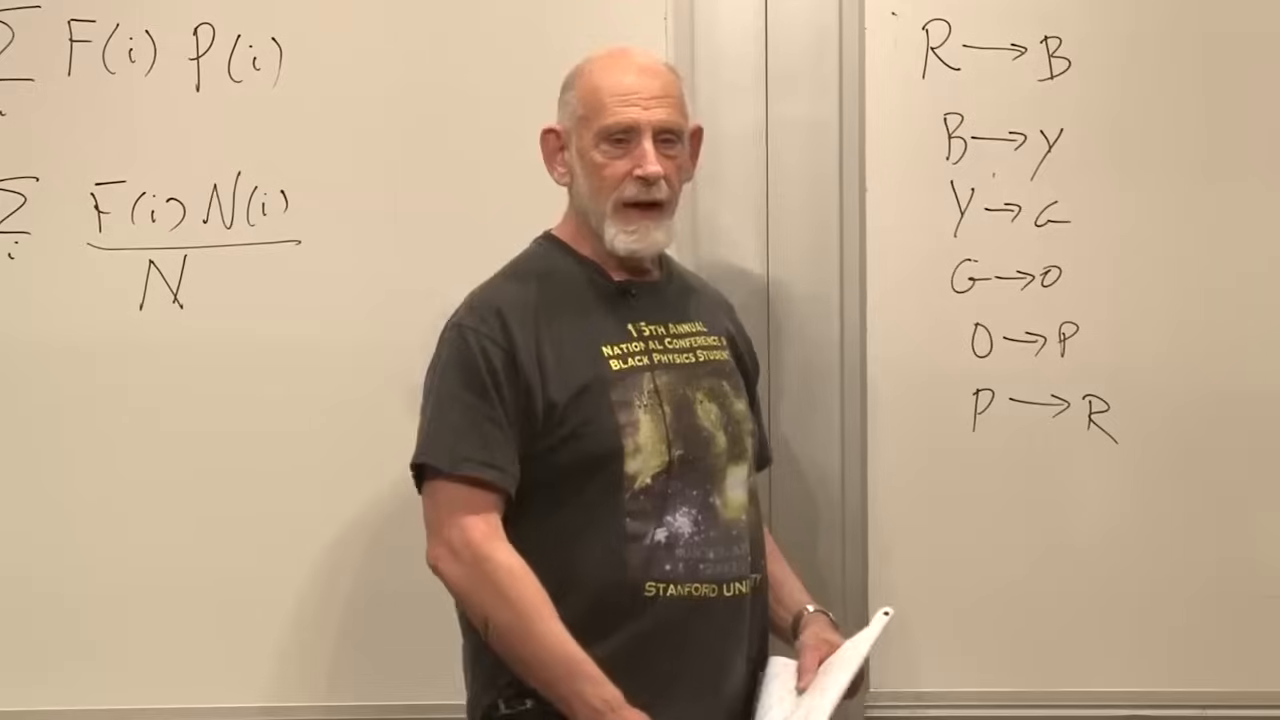
\includegraphics[width=0.92\textwidth]{lecture_01_figure_02.png}
Les formules des valeurs moyennes restent affichées sur le tableau de gauche, tandis que les six mises à jour déterministes des couleurs sont énumérées sur celui de droite.\caption{
}
\lectureframe{00:26:28}
\end{figure}

La liste au tableau se comprend mieux sous la forme d’un cycle orienté :
\begin{figure}[htbp]
\centering
\begin{tikzpicture}[
  >=Latex,
  state/.style={draw,circle,minimum size=8mm,inner sep=1pt}
]
\node[state] (R) at (90:2.2) {$R$};
\node[state] (B) at (30:2.2) {$B$};
\node[state] (Y) at (-30:2.2) {$Y$};
\node[state] (G) at (-90:2.2) {$G$};
\node[state] (O) at (-150:2.2) {$O$};
\node[state] (P) at (150:2.2) {$P$};
\draw[->] (R) -- (B);
\draw[->] (B) -- (Y);
\draw[->] (Y) -- (G);
\draw[->] (G) -- (O);
\draw[->] (O) -- (P);
\draw[->] (P) -- (R);
\end{tikzpicture}
Une orbite unique à six états. Chaque état est visité une fois par période.\caption{
}
\label{fig:sm1-six-cycle}
\end{figure}

Supposons que nous ignorions l’état initial et que nous observions le système à un instant inconnu. Chaque étape ayant la même durée, le système passe un sixième de la période dans chaque couleur :
\begin{equation}
 p(R)=p(B)=p(Y)=p(G)=p(O)=p(P)=\frac16.
 \label{eq:sm1-uniform-cycle}
\end{equation}
Cette égalité ne découle pas de la forme de l’objet. Elle vient du temps passé dans chaque état, qui est le même.

Nous pouvons réordonner les flèches et obtenir une loi microscopique différente tout en conservant un cycle unique à six états. La séquence détaillée change, mais la probabilité d’observer le système reste \(1/6\), puisque chaque état apparaît toujours une fois par période. Cette prédiction ne dépend donc ni du point de départ ni de l’ordre détaillé. Elle dépend uniquement de la structure de l’orbite et de la même durée pour chaque étape.

\begin{classroomqa}
\classquestion{Si l’objet n’est pas symétrique, en quel sens est-il
légitime d’attribuer à chaque couleur la probabilité \(1/6\) ?}
\lecturerresponse{Cette attribution découle de la dynamique, et non de la géométrie. Une observation faite à une phase inconnue d’une orbite à six étapes échantillonne six intervalles de temps égaux. L’équivalence pertinente est celle des positions sur l’orbite, et non celle des faces de l’objet. Si les durées de séjour étaient différentes, les probabilités le seraient aussi.
\lecturetimestamp{00:27:11--00:29:49}}
\end{classroomqa}

\section{Cycles disjoints et grandeurs conservées}

Une loi déterministe ne place pas nécessairement tous les états sur une seule orbite. Considérons deux cycles disjoints,
\begin{equation}
 R\longrightarrow B\longrightarrow G\longrightarrow R,
 \qquad
 P\longrightarrow Y\longrightarrow O\longrightarrow P.
 \label{eq:sm1-two-cycles}
\end{equation}
Si nous savons que le système se trouve sur le premier cycle, alors
\begin{equation}
 \begin{aligned}
 p(R)=p(B)=p(G)&=\frac13,\\
 p(P)=p(Y)=p(O)&=0.
 \end{aligned}
\end{equation}
Savoir qu’il se trouve sur le second cycle inverse ces attributions.

Le cas général nécessite des poids a priori. Étiquetons les cycles \(+1\) et
\(-1\), et notons leurs probabilités \(p_+\) et \(p_-\), avec
\begin{equation}
 p_++p_-=1.
\end{equation}
Alors
\begin{align}
 p(R)=p(B)=p(G)&=\frac{p_+}{3},\\
 p(P)=p(Y)=p(O)&=\frac{p_-}{3}.
 \label{eq:sm1-sector-weights}
\end{align}
Les facteurs \(1/3\) découlent du mouvement au sein d’un cycle. Les nombres \(p_+\)
et \(p_-\) n’en découlent pas. Ils doivent provenir d’une connaissance supplémentaire, par exemple d’une autre expérience ou d’un autre système qui sélectionne le secteur initial.

Les étiquettes \(+1\) et \(-1\) définissent une grandeur conservée : si le système commence sur un cycle, la loi d’évolution ne le transporte jamais sur l’autre. On peut appeler cette grandeur énergie ou lui donner un nom provisoire comme \emph{zilch}. Son nom importe peu. La conservation signifie que l’espace des états est partitionné en régions que la dynamique ne peut traverser.

Les cycles n’ont pas besoin de contenir le même nombre d’états. Une orbite à quatre états et une orbite à deux états définissent tout de même deux secteurs conservés. Un échantillonnage uniforme dans le temps donne alors \(1/4\) dans le premier secteur et \(1/2\) dans le second, dans chaque cas multiplié par la probabilité a priori de ce secteur. La mécanique statistique doit répondre à deux questions logiquement distinctes :
\begin{enumerate}
\item Pour un secteur conservé donné, combien de temps la dynamique passe-t-elle dans chacun de ses états ?
\item Quelle probabilité attribuer au secteur conservé lui-même ?
\end{enumerate}

\begin{classroomqa}
\audiencequestion{Supposons-nous que tous les états d’un même secteur
conservé reçoivent la même probabilité ?}
\lecturerresponse{Pour les lois discrètes simplifiées présentées ici, oui, car chaque état dure le même intervalle de temps et le mouvement est déterministe. L’incertitude porte sur la phase initiale de l’orbite. Un détecteur dont la résolution temporelle est de l’ordre de la milliseconde ne peut pas résoudre des mises à jour qui se produisent à l’échelle de la microseconde, même si un instantané suffisamment rapide peut toujours identifier l’état observé. Dans un système plus général, il faut tenir compte explicitement des durées de séjour inégales.
\lecturetimestamp{00:36:16--00:37:17}}
\end{classroomqa}

\begin{classroomqa}
\audiencequestion{Si deux instantanés sont pris et que le premier identifie un
cycle, le second devrait-il identifier le même cycle ?}
\lecturerresponse{Oui. C’est précisément ce que signifie la conservation. Une fois qu’une mesure détermine la valeur de la grandeur conservée, les probabilités futures peuvent être conditionnées par cette valeur, et la probabilité des états de l’autre secteur devient nulle.
\lecturetimestamp{00:37:18--00:37:45}}
\end{classroomqa}

\subsection{Énergie partagée entre deux systèmes}

Remplaçons maintenant l’étiquette abstraite par l’énergie. Une boîte isolée est un système fermé dont l’énergie se conserve. Deux boîtes isolées possèdent deux énergies conservées séparément, puisqu’elles n’interagissent pas. Relions-les par un passage étroit qui permet à l’énergie de circuler : les énergies individuelles peuvent alors varier, tandis que leur somme reste constante.

\begin{figure}[htbp]
\centering
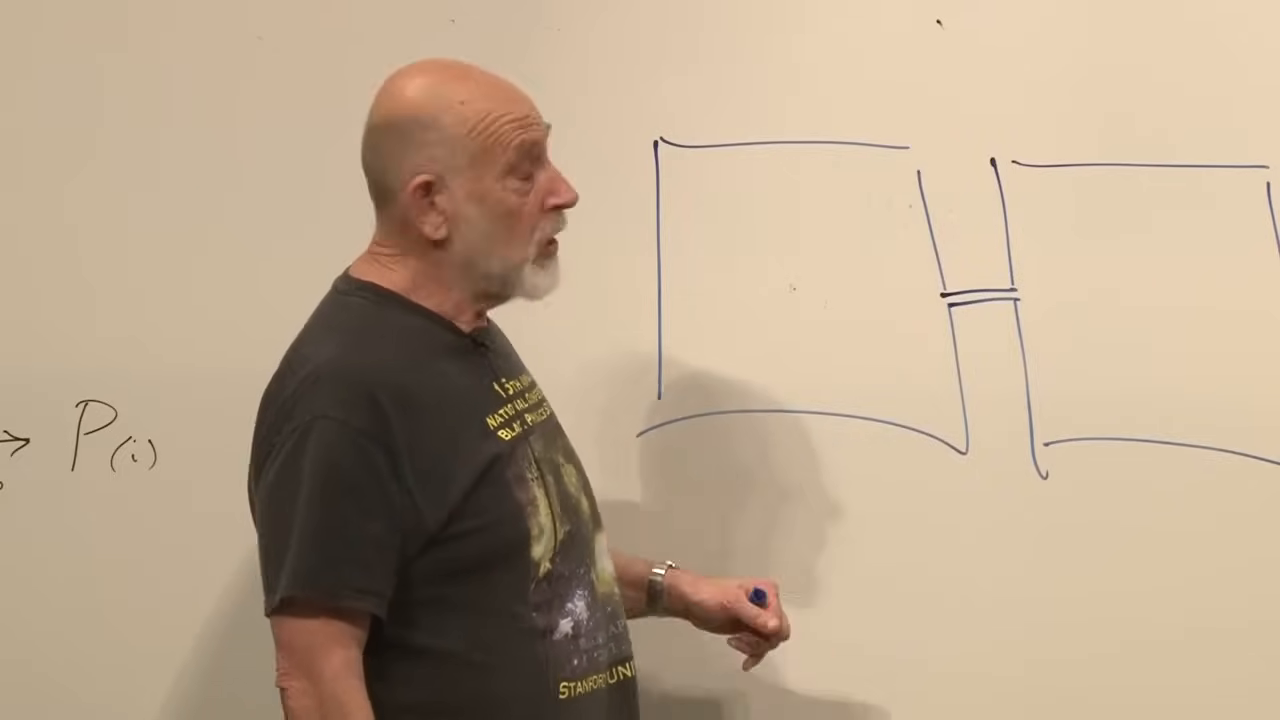
\includegraphics[width=0.92\textwidth]{lecture_01_figure_03.png}
Deux sous-systèmes reliés par un canal étroit par lequel l’énergie peut circuler.\caption{
}
\lectureframe{00:39:19}
\end{figure}

\begin{figure}[htbp]
\centering
\begin{tikzpicture}[>=Latex]
\draw[thick,rounded corners=4pt] (-4,1.8) rectangle (-0.7,-1.5);
\draw[thick,rounded corners=4pt] (0.7,1.5) rectangle (4,-1.8);
\draw[thick] (-0.7,0.45) -- (0.7,0.45);
\draw[thick] (-0.7,-0.35) -- (0.7,-0.35);
\draw[<->,very thick] (-0.45,0.05) -- (0.45,0.05);
\node at (-2.35,0.15) {subsystem \(1\)};
\node at (2.35,-0.15) {subsystem \(2\)};
\node[above] at (0,0.5) {energy exchange};
\end{tikzpicture}
\caption{Une fois la connexion établie, seule \(E_1+E_2\) est conservée.
La répartition de l’énergie devient un problème de probabilité.}
\label{fig:sm1-connected-systems}
\end{figure}

Étant donnée une énergie totale, nous pouvons demander quelle est la probabilité que le sous-système \(1\) ait une énergie \(E_1\), tandis que le sous-système \(2\) possède le reste. Des boîtes identiques devraient avoir la même énergie moyenne, mais la moyenne ne décrit pas toute la distribution. Pour déterminer les probabilités d’un sous-système, on peut donc l’inclure dans un système fermé plus grand, dont la loi de conservation fournit l’information manquante. Cette construction reviendra tout au long de la mécanique statistique.

\section{Bonnes lois, mauvaises lois et loi moins un}

Toute règle d’évolution déterministe n’est pas admissible comme loi fondamentale. Considérons l’application
\begin{equation}
 \begin{aligned}
 R&\mapsto R,& B&\mapsto R,& Y&\mapsto R,\\
 G&\mapsto R,& O&\mapsto R,& P&\mapsto R.
 \end{aligned}
 \label{eq:sm1-all-to-red}
\end{equation}
Elle prédit parfaitement l’avenir : après une étape, l’état est rouge. En revanche, elle échoue dans le sens opposé. Une fois le système à l’état rouge, rien n’indique s’il vient de l’état bleu, jaune, vert, orange ou violet, ou s’il était déjà rouge.

\begin{figure}[htbp]
\centering
\begin{tikzpicture}[
  >=Latex,
  state/.style={draw,circle,minimum size=8mm,inner sep=1pt}
]
\node[state,fill=red!12] (R) at (0,0) {$R$};
\node[state] (B) at (-3,1.6) {$B$};
\node[state] (Y) at (-3,0) {$Y$};
\node[state] (G) at (-3,-1.6) {$G$};
\node[state] (O) at (3,1.6) {$O$};
\node[state] (P) at (3,-1.6) {$P$};
\draw[->] (B) -- (R);
\draw[->] (Y) -- (R);
\draw[->] (G) -- (R);
\draw[->] (O) -- (R);
\draw[->] (P) -- (R);
\draw[->,loop above] (R) to (R);
\end{tikzpicture}
Une loi plusieurs-vers-un prédit l’état suivant, mais efface les distinctions entre les états passés possibles.\caption{
}
\label{fig:sm1-bad-law}
\end{figure}

À l’inverse, un cycle fermé préserve la trace. Si le temps écoulé est connu, nous pouvons faire évoluer l’état vers l’avenir ou vers le passé, même après plusieurs milliers de périodes. La loi préserve les distinctions entre les conditions initiales. Susskind appelle cette exigence la \emph{loi moins un de la physique} : l’information n’est pas fondamentalement perdue.

Pour un espace d’états fini et discret, le critère graphique est simple :
\begin{quote}
Chaque état d’une bonne loi possède exactement une flèche sortante et exactement une flèche entrante.
\end{quote}
La flèche sortante détermine l’avenir ; la flèche entrante permet de reconstituer le passé. Mathématiquement, la mise à jour est une permutation des états.

\subsection{Le frottement n’est qu’un contre-exemple apparent}

Le théorème de Liouville est son analogue continu. Le frottement semble le contredire. Faisons glisser une gomme sur une table : quel que soit son point de départ, elle finit par s’immobiliser. Une équation schématique de la force de frottement est
\begin{equation}
 m\ddot x=-\gamma\dot x,
 \qquad \gamma>0.
 \label{eq:sm1-drag}
\end{equation}
Sa vitesse décroît exponentiellement. Si cette équation était la loi fondamentale de chaque particule dans une pièce hermétiquement close, tout mouvement finirait par disparaître, la température tomberait à zéro et de nombreux états initiaux s’effondreraient en un seul état final. La conservation de l’énergie échouerait, l’information disparaîtrait et le désordre diminuerait. Ce serait, dans le cas continu, comme si tout finissait à l’état rouge.

Le frottement réel ne produit pas cet effet. La gomme chauffe la table, elle-même et l’environnement alentour. Les positions et quantités de mouvement microscopiques conservent la trace des distinctions perdues dans le mouvement visible. Le frottement est une équation effective pour un sous-système, obtenue après omission des degrés de liberté inobservés ; ce n’est pas une loi dissipative fondamentale décrivant le système fermé dans son ensemble.

\begin{classroomqa}
\classquestion{Que représente l’équation différentielle
\(m\ddot x=-\gamma\dot x\), et pourquoi ne peut-elle pas être une loi fondamentale
d’un système fermé ?}
\lecturerresponse{Elle représente le frottement visqueux. À elle seule, elle entraîne toutes les vitesses vers zéro, ce qui ferait refroidir un gaz jusqu’à zéro, quelle que soit sa température initiale. Dans une description réelle d’un système fermé, l’énergie mécanique et l’information perdues passent dans des degrés de liberté microscopiques. L’équation de frottement n’est fiable qu’après élimination de ces variables.
\lecturetimestamp{00:44:40--00:48:56}}
\end{classroomqa}

\section{États occupés et première entropie}

La conservation de l’information possède un équivalent probabiliste. Supposons que \(M\) états parmi \(N\) reçoivent une probabilité égale,
\begin{equation}
 p_i=
 \begin{cases}
 1/M, & i\text{ in the occupied set},\\
 0, & i\text{ outside it}.
 \end{cases}
 \label{eq:sm1-uniform-occupied}
\end{equation}
Une évolution qui préserve l’information peut redistribuer les états occupés, mais elle ne peut pas les fusionner. À tout instant ultérieur, il reste \(M\) états de probabilité \(1/M\). En revanche, la mauvaise application \eqref{eq:sm1-all-to-red} peut réduire plusieurs états occupés à un seul.

Le nombre \(M\) mesure l’ignorance. Si \(M=N\), tous les états sont possibles et notre ignorance est maximale. Si \(M=1\), l’état microscopique est connu avec exactitude. La première définition de l’entropie est donc
\begin{equation}
 S=\log M.
 \label{eq:sm1-entropy-logm}
\end{equation}
On obtient
\begin{equation}
 S_{\max}=\log N,
 \qquad
 S_{\min}=0.
\end{equation}
Si l’espace des états est infini, il n’existe pas nécessairement de borne supérieure finie.

Dans ce développement, l’entropie apparaît avant la température, et même avant l’énoncé formel de la conservation de l’énergie. En ce sens, elle est plus primitive. Pourtant, elle n’est pas une propriété du seul système mécanique. Elle dépend à la fois du système et de la distribution de probabilité qui représente ce que l’on sait. Des observateurs disposant d’informations différentes peuvent attribuer des entropies différentes au même système mécanique.

Sous l’évolution microscopique exacte, les états occupés sont simplement réarrangés ; cette entropie à grain fin se conserve donc. En pratique, nous perdons la trace du temps, négligeons les corrélations et ne suivons pas un nombre immense de variables. Notre distribution de probabilité s’étale alors sur un plus grand nombre de possibilités, et l’entropie attribuée à la description macroscopique augmente. Les équations n’ont pas besoin de détruire l’information pour que notre description exploitable en perde.

\begin{classroomqa}
\classquestion{Quelle est l’entropie maximale possible d’un système fini
comportant \(N\) états ?}
\lecturerresponse{C’est \(\log N\) ; elle est atteinte lorsque les \(N\) états sont tous équiprobables. L’entropie minimale est zéro ; elle est atteinte lorsqu’un état a une probabilité égale à un. L’entropie mesure donc à la fois l’état de nos connaissances et l’espace des états accessibles.
\lecturetimestamp{00:56:46--00:58:19}}
\end{classroomqa}

\section{Écoulement de Liouville dans l’espace des phases continu}

Pour des particules dont les positions et les quantités de mouvement sont continues, un état microscopique est un point de l’espace des phases. Nous notons les coordonnées \(q_a\) et leurs moments conjugués \(p_a\). Avec un grand nombre de particules, les axes sont extraordinairement nombreux ; un dessin en deux dimensions comportant un \(q\) et un \(p\) n’est qu’une représentation simplifiée. L’espace des phases est de dimension paire, car chaque coordonnée a un moment qui lui est associé.

Supposons que notre connaissance soit représentée par une région \(\Omega_0\) : la densité de probabilité est uniforme à l’intérieur de cette région et nulle à l’extérieur. Par exemple, savoir que chaque particule se trouve dans la pièce restreint les coordonnées de position, tandis que des bornes sur leurs vitesses restreignent les coordonnées de moment.

L’évolution hamiltonienne entraîne chaque point de l’espace des phases le long d’une trajectoire. Des points voisins restent voisins, et la région occupée s’écoule comme une parcelle de fluide incompressible :
\begin{figure}[htbp]
\centering
\begin{tikzpicture}[>=Latex,scale=0.95]
\draw[->] (-4.2,0) -- (4.3,0) node[right] {$q$};
\draw[->] (-3.7,-2.2) -- (-3.7,2.4) node[above] {$p$};
\draw[fill=blue!12,thick]
  (-3.0,-0.5) .. controls (-2.7,1.0) and (-1.3,1.2) .. (-0.9,0.1)
  .. controls (-0.6,-1.0) and (-2.2,-1.4) .. cycle;
\node at (-1.9,0.0) {$\Omega_0$};
\draw[->,very thick] (-0.3,0.2) -- (0.8,0.2);
\draw[fill=orange!15,thick]
  (1.2,-1.1) .. controls (1.5,0.3) and (2.3,1.8) .. (3.2,1.1)
  .. controls (3.6,0.7) and (2.8,-0.4) .. (2.5,-1.5)
  .. controls (2.1,-1.8) and (1.5,-1.6) .. cycle;
\node at (2.35,0.1) {$\Omega_t$};
\end{tikzpicture}
L’écoulement hamiltonien peut étirer et cisailler une région occupée de l’espace des phases, mais il en conserve le volume.\caption{
}
\label{fig:sm1-liouville-flow}
\end{figure}

Le théorème de Liouville énonce que
\begin{equation}
 \operatorname{Vol}(\Omega_t)
 =
 \operatorname{Vol}(\Omega_0).
 \label{eq:sm1-liouville-volume}
\end{equation}
Si la densité initiale est uniforme sur \(\Omega_0\), la densité transportée est uniforme sur \(\Omega_t\). C’est l’analogue continu de la conservation du nombre et des poids des états discrets occupés.

Le théorème résout aussi géométriquement le problème du frottement. Si nous ne considérons que la quantité de mouvement visible de la gomme, un nuage de possibilités semble se resserrer vers \(p=0\). Dans l’espace des phases complet, le nuage s’étale dans les positions et les quantités de mouvement des molécules de la gomme et de la table. Une projection peut se contracter tandis que le volume total de l’espace de grande dimension reste constant.

\begin{classroomqa}
\classquestion{Si toutes les trajectoires visibles tendent vers le repos, la
région occupée de l’espace des phases s’est-elle effondrée sur l’axe \(p=0\) ?}
\lecturerresponse{Uniquement dans la projection réduite. Le système complet
comprend les variables microscopiques de la table, de la gomme et de l’environnement. À mesure que l’intervalle des quantités de mouvement visibles se resserre, la distribution s’étale dans ces directions cachées. Le théorème de Liouville s’applique à l’espace des phases complet du système fermé, et non à un ensemble incomplet de variables macroscopiques.
\lecturetimestamp{01:04:37--01:06:29}}
\end{classroomqa}

\section{De la loi moins un au premier principe}

\subsection{Bref aperçu du principe zéro}

Avant d’énoncer le premier principe, il est utile de nommer le principe zéro. L’équilibre thermique n’a pas encore été défini ; pour l’instant, le principe se limite à un énoncé structurel :
\begin{quote}
Si le système \(A\) est en équilibre thermique avec \(B\), et si \(B\) est en équilibre thermique avec \(C\), alors \(A\) est en équilibre thermique avec \(C\).
\end{quote}
Cette transitivité permettra plus tard de définir la température. Pour le moment, nous la laissons de côté.

\subsection{Conservation de l’énergie}

Le premier principe pour un système fermé s’écrit simplement
\begin{equation}
 \frac{dE}{dt}=0.
 \label{eq:sm1-first-law}
\end{equation}
Cette forme concise dissimule toute sa portée. L’énergie est une grandeur conservée, et le terme « énergie » prendra plus tard un sens thermodynamique plus riche.

Si un système fermé est constitué de deux parties et que leurs énergies sont additives,
\begin{equation}
 E=E_1+E_2,
\end{equation}
alors
\begin{equation}
 \frac{dE_1}{dt}+\frac{dE_2}{dt}=0,
 \qquad\text{or}\qquad
 \frac{dE_1}{dt}=-\frac{dE_2}{dt}.
 \label{eq:sm1-energy-exchange}
\end{equation}
La seconde forme rend l’échange explicite : l’énergie perdue par un sous-système est gagnée par l’autre.

L’hypothèse d’additivité demande quelques précautions. Deux particules en interaction gravitationnelle possèdent chacune une énergie cinétique, mais leur interaction ajoute une énergie potentielle qui appartient à la paire. L’énergie totale se conserve, même si elle ne peut pas s’écrire exactement comme la somme de l’énergie de l’une et de celle de l’autre.

La thermodynamique autorise souvent une excellente approximation additive, car l’énergie globale est proportionnelle au volume, tandis que l’énergie d’interaction à courte portée entre de grands éléments voisins dépend surtout de leur aire de contact. Divisons une grande table en blocs : l’énergie interne de chaque bloc est un effet de volume, tandis que le couplage entre blocs adjacents est un effet de surface. Pour de grands blocs, ce dernier est relativement faible. L’équation
\eqref{eq:sm1-first-law} est exacte pour l’ensemble fermé ; la forme exprimée pour les sous-systèmes,
\eqref{eq:sm1-energy-exchange}, suppose que l’énergie d’interaction est négligeable.

\begin{classroomqa}
\audiencequestion{La normalisation \(\sum_i p_i=1\) suppose-t-elle aussi que
les issues énumérées sont mutuellement exclusives ?}
\lecturerresponse{Oui. L’étiquette d’un état est définie de sorte que les possibilités ne se recouvrent pas : si le dé est dans l’état jaune, il n’est pas simultanément dans l’état rouge. Dans le langage courant, on peut mélanger les couleurs, mais la partition des états utilisée dans le calcul des probabilités doit être constituée d’issues mutuellement exclusives.
\lecturetimestamp{01:12:14--01:12:55}}
\end{classroomqa}

\section{Retour à l’entropie}

Le cours revient maintenant explicitement à une question laissée en suspens. Bien que familière à nos sens, la température est une grandeur dérivée. L’entropie et l’énergie doivent être établies avant que l’on puisse définir proprement la température.

\subsection{Distributions de probabilité générales}

La définition particulière \(S=\log M\) s’applique lorsque \(M\) états sont équiprobables et que tous les autres ont une probabilité nulle. Une distribution générale n’est pas nécessairement rectangulaire. Ses poids peuvent varier de façon régulière ou irrégulière selon les étiquettes des états.

\begin{figure}[htbp]
\centering
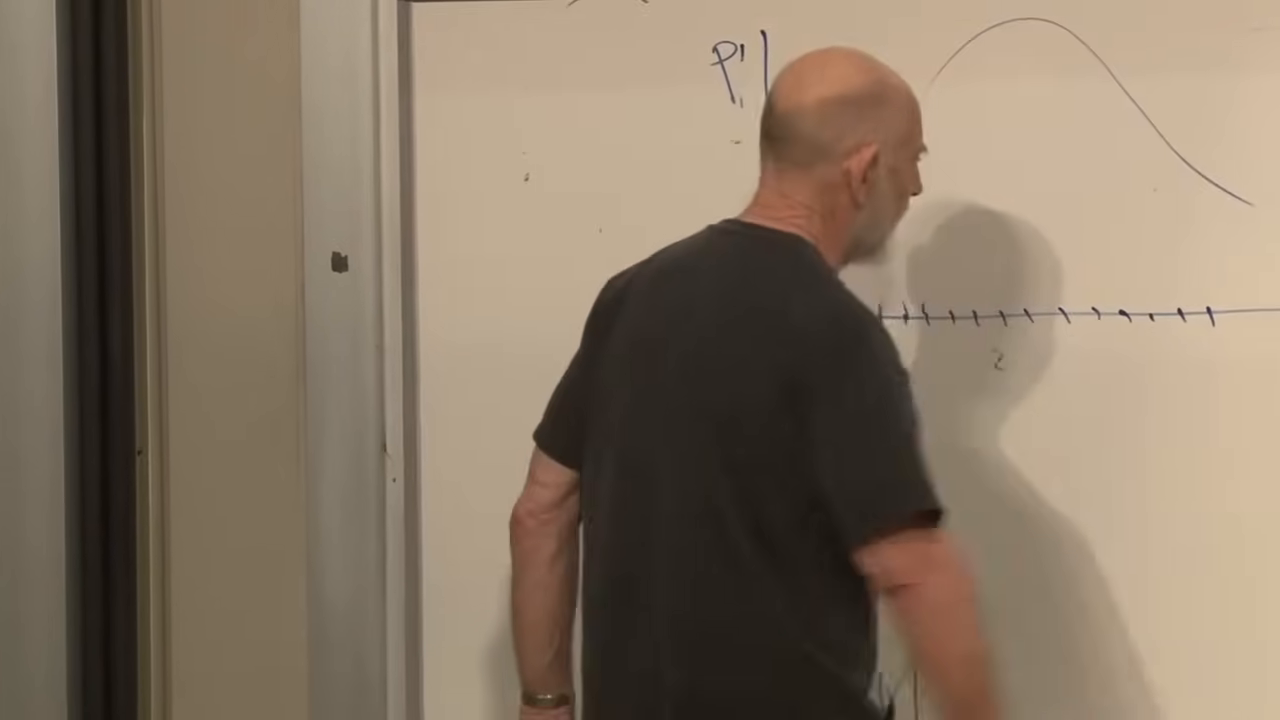
\includegraphics[width=0.92\textwidth]{lecture_01_figure_05.png}
Une distribution de probabilité représentée sur des étiquettes d’états discrètes. Pour l’entropie, c’est l’étendue, et non la courbe précise, qui importe.\caption{
}
\lectureframe{01:14:40}
\end{figure}

\begin{figure}[htbp]
\centering
\resizebox{\linewidth}{!}{%
\begin{tikzpicture}[>=Latex,scale=0.93]
\draw[->] (-4.2,0) -- (4.4,0) node[right] {state label \(i\)};
\draw[->] (-4,0) -- (-4,3.2) node[above] {$p_i$};
\foreach \x in {-3.6,-3.1,...,3.6}
  \draw (\x,0.08) -- (\x,-0.08);
\draw[very thick]
  plot[smooth] coordinates {
  (-3.7,0.12) (-3.0,0.28) (-2.3,0.72) (-1.6,1.45)
  (-0.9,2.25) (-0.2,2.65) (0.5,2.28) (1.2,1.55)
  (1.9,0.88) (2.7,0.38) (3.5,0.14)};
\draw (-1.8,-0.18) -- (-1.8,-0.5);
\draw (1.8,-0.18) -- (1.8,-0.5);
\draw[<->] (-1.8,-0.46) -- (1.8,-0.46);
\node at (0,-0.82) {effective spread};
\end{tikzpicture}
}
Une distribution étroite comporte moins d’incertitude qu’une distribution large. L’entropie doit mesurer la distribution dans son ensemble.\caption{
}
\label{fig:sm1-probability-spread}
\end{figure}

La définition générale est
\begin{equation}
 S=-\sum_i p_i\log p_i.
 \label{eq:sm1-shannon-entropy}
\end{equation}
En utilisant \eqref{eq:sm1-expectation}, on obtient
\begin{equation}
 S=-\langle\log p\rangle.
\end{equation}
Le signe moins compense le fait que \(\log p_i<0\) lorsque
\(0<p_i<1\).

\subsection{Retrouver le résultat uniforme}

Il faut vérifier que la formule générale reproduit la première définition.
Pour un état inoccupé, \(p_i=0\) alors que \(\log p_i\) diverge. Le produit
admet la limite bien définie
\begin{equation}
 \lim_{p\to0^+}p\log p=0.
 \label{eq:sm1-plogp-limit}
\end{equation}
Ainsi, les états de probabilité nulle ne contribuent pas.

\begin{classroomqa}
\audiencequestion{Si \(p_i=0\), le terme s’annule-t-il vraiment ? Le logarithme
de zéro vaut moins l’infini.}
\lecturerresponse{Le terme est défini par la limite
\(\lim_{p\to0^+}p\log p\), qui vaut zéro. Le facteur \(p\) tend vers zéro
plus rapidement que le logarithme ne diverge. Ainsi, les états arbitrairement improbables apportent des contributions arbitrairement faibles, et un état strictement impossible ne contribue pas.
\lecturetimestamp{01:18:27--01:19:46}}
\end{classroomqa}

Pour chacun des \(M\) états occupés, \(p_i=1/M\). On a donc
\begin{align}
 S
 &=-\sum_{\mathrm{occupied}\ i}
 \frac1M\log\!\left(\frac1M\right)\\
 &=-M\frac1M\log\!\left(\frac1M\right)\\
 &=-\log\!\left(\frac1M\right)
 =\log M.
 \label{eq:sm1-entropy-check}
\end{align}
L’expression générale coïncide exactement avec l’expression particulière. Une distribution plus étalée accorde un poids appréciable à davantage de possibilités et a donc une entropie plus élevée ; une distribution plus resserrée a une entropie plus faible.

\begin{figure}[htbp]
\centering
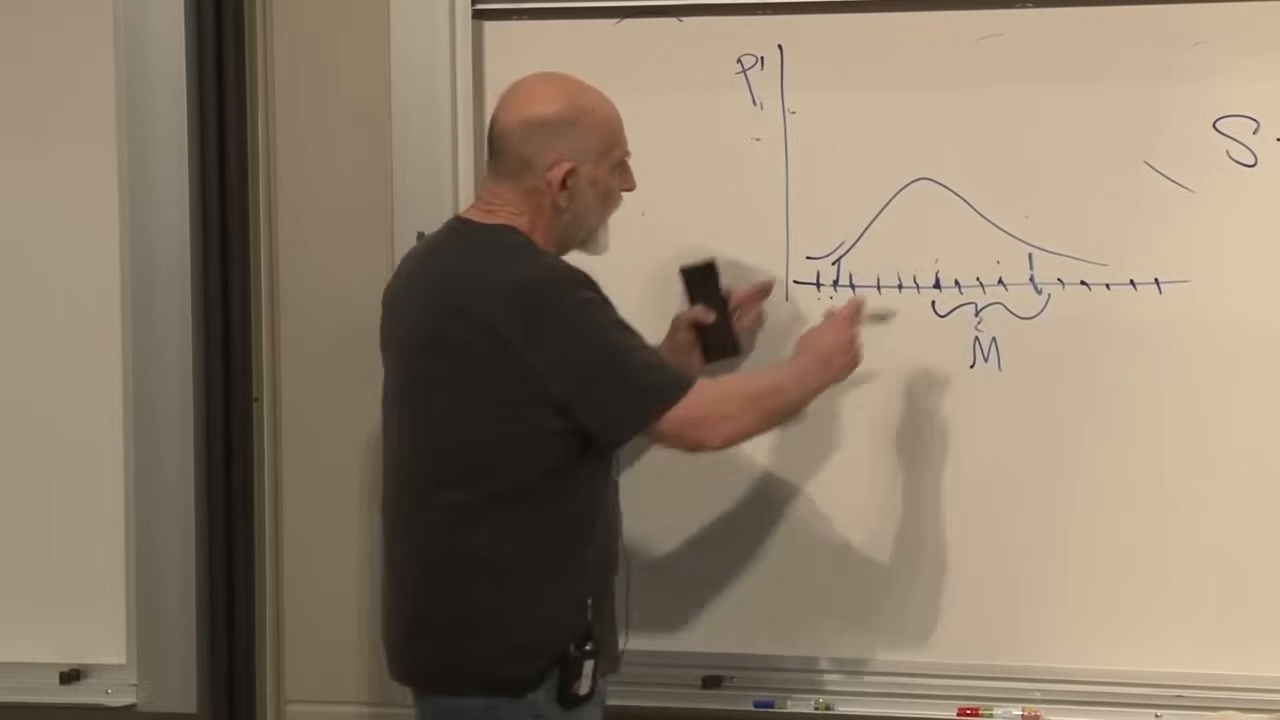
\includegraphics[width=0.92\textwidth]{lecture_01_figure_06.png}
\caption{La largeur indiquée \(M\) souligne le lien entre l’étalement des probabilités significatives et l’entropie.}
\lectureframe{01:16:42}
\end{figure}

L’entropie est associée à une distribution de probabilité sur l’espace des états. Ce n’est pas une observable prise isolément, comme l’énergie ou la quantité de mouvement d’un microétat. Un état exact peut être représenté par une distribution concentrée sur cet état ; son entropie est alors nulle. Mais l’entropie change lorsque l’état de connaissance change.

\section{Pièces, bits et dénombrement explicite}

Soit \(n\) le nombre de pièces. Le nombre de configurations microscopiques est
\begin{equation}
 N=2^n.
 \label{eq:sm1-coin-state-count}
\end{equation}
Si l’on ne sait rien des pièces, les \(2^n\) configurations sont toutes équiprobables, et
\begin{equation}
 S_{\max}=\log(2^n)=n\log2.
 \label{eq:sm1-coin-max-entropy}
\end{equation}
L’entropie est additive en fonction du nombre de pièces indépendantes.

Avec des logarithmes en base \(2\), un système à deux états totalement inconnu a une entropie d’un bit. Avec des logarithmes népériens, son entropie vaut \(\log2\). L’unité est conventionnelle ; l’ordre sous-jacent et l’additivité restent inchangés.

À l’autre extrême, si l’on connaît l’état de chaque pièce, une seule configuration a une probabilité égale à un :
\begin{equation}
 S=0.
\end{equation}
Plus on dispose d’informations, plus l’entropie est faible.

Supposons maintenant qu’exactement une des \(n\) pièces soit côté pile et que toutes les autres soient côté face, sans que l’on sache où se trouve celle qui est côté pile. Il y a \(n\) configurations équiprobables, une pour chaque position possible de cette pièce, donc
\begin{equation}
 S=\log n.
 \label{eq:sm1-one-tail-entropy}
\end{equation}
Ce n’est généralement pas un multiple entier de \(\log2\). Le bit est une unité pratique ; cela ne signifie pas que toute entropie soit un nombre entier de bits.

\begin{classroomqa}
\audiencequestion{\(\log2\) n’apparaît-il que parce que chaque pièce a deux états possibles ? Un élément à trois états donnerait-il \(\log3\) ?}
\lecturerresponse{Exactement. Un élément dont l’état est uniformément inconnu parmi \(k\) états possibles contribue \(\log k\). Les commutateurs binaires sont particulièrement pratiques dans les ordinateurs, car les commutateurs physiques réalisent naturellement deux états stables et parce que deux est le plus petit entier non trivial.
\lecturetimestamp{01:29:55--01:30:48}}
\end{classroomqa}

\begin{classroomqa}
\audiencequestion{Quelle base faut-il utiliser pour le logarithme ?}
\lecturerresponse{Dans ces formules de physique, \(\log\) désigne le logarithme népérien. Les théoriciens de l’information utilisent souvent la base \(2\) ; l’entropie est alors directement exprimée en bits. Changer de base multiplie toutes les entropies par un même facteur de conversion et ne modifie aucune conclusion physique.
\lecturetimestamp{01:30:49--01:32:06}}
\end{classroomqa}

\section{Entropie dans l’espace des phases continu}

Revenons à un espace des phases classique \(\Gamma\). Si la densité de probabilité est uniforme dans une région de volume \(V_\Gamma\) et nulle à l’extérieur, l’analogue du dénombrement de \(M\) états équiprobables est
\begin{equation}
 S=\log\!\left(\frac{V_\Gamma}{V_0}\right).
 \label{eq:sm1-continuous-uniform}
\end{equation}
Ici, \(V_\Gamma\) est le volume dans l’espace complet, de grande dimension, des coordonnées et des quantités de mouvement, et non un volume spatial ordinaire. Le volume fixe \(V_0\) est une cellule de référence de l’espace des phases qui rend le logarithme sans dimension. En posant \(V_0=1\), on obtient l’écriture abrégée \(S=\log V_\Gamma\) utilisée au tableau.

Pour une densité de probabilité générale \(P(q,p)\), la somme discrète devient une intégrale sur l’espace des phases. La normalisation s’écrit
\begin{equation}
 \int_\Gamma d\Gamma\,P(q,p)=1,
 \label{eq:sm1-continuous-normalization}
\end{equation}
et l’entropie
\begin{equation}
 S=-\int_\Gamma d\Gamma\,
 P(q,p)\log\!\bigl[P(q,p)V_0\bigr].
 \label{eq:sm1-continuous-entropy}
\end{equation}
La densité est une probabilité par cellule de l’espace des phases. Conceptuellement,
\eqref{eq:sm1-continuous-entropy} mesure toujours l’étalement de la distribution de probabilité ; pour un domaine uniforme, elle se réduit au logarithme du volume occupé, exprimé en unités de la cellule de référence. Modifier cette cellule fixe décale toutes les entropies continues d’une même constante additive et laisse inchangées leurs différences.

\begin{classroomqa}
\audiencequestion{Pourquoi le symbole de coordonnée passe-t-il de \(x\) à \(q\) ?}
\lecturerresponse{Il n’y a aucun changement physique. En mécanique classique, on utilise couramment \(x\) ou \(q\) pour les coordonnées et \(p\) pour les quantités de mouvement conjuguées. Le changement de notation n’était qu’un lapsus ; la construction de l’espace des phases reste la même.
\lecturetimestamp{01:37:10--01:37:39}}
\end{classroomqa}

La température et la distribution de Boltzmann sont volontairement abordées plus tard. La prochaine étape consistera à définir l’équilibre thermique, puis à identifier la distribution de probabilité qui lui correspond.

\section{Questions sur la corrélation, l’additivité et l’information}

\subsection{La corrélation signifie qu’une mesure modifie une autre distribution}

Lorsqu’on ignore tout de pièces indépendantes, on attribue la même probabilité à chaque configuration. Mesurer l’une des pièces n’apprend alors rien sur les autres. Leurs distributions restent inchangées.

L’ensemble à une seule pièce côté pile est différent. Si la pièce mesurée est côté pile, toutes les autres sont certainement côté face. Si la pièce mesurée est côté face, la seule pièce côté pile doit se trouver parmi les \(n-1\) restantes ; chaque position restante a donc une probabilité conditionnelle de
\begin{equation}
\begin{aligned}
 p(&\text{tail at a specified remaining position}\\
   &\mid\text{measured head})=\frac{1}{n-1}.
\end{aligned}
 \label{eq:sm1-conditional-tail}
\end{equation}
C’est cela, la corrélation : apprendre la valeur d’une variable modifie la distribution de probabilité attribuée à une autre.

\begin{classroomqa}
\audiencequestion{Dans les exemples d’entropie, a-t-on supposé que les pièces étaient indépendantes ?}
\lecturerresponse{Seulement lorsque l’ignorance complète était représentée par des probabilités égales pour les \(2^n\) configurations. Dans ce cas, mesurer une pièce ne modifie pas les distributions des autres. L’exemple à une seule pièce côté pile présente explicitement une corrélation : une mesure actualise ce qui est possible ailleurs. C’est l’information énoncée qui détermine la distribution de probabilité utilisée.
\lecturetimestamp{01:38:43--01:41:58}}
\end{classroomqa}

L’exemple des cycles disjoints a la même structure logique. Mesurer l’étiquette conservée \(+1\) ou \(-1\) restreint tous les états ultérieurs à un seul secteur. Conditionner la distribution sur l’information conservée modifie les états admissibles.

L’entropie est additive pour des systèmes non corrélés. Si
\begin{equation}
 p_{ij}=p_i^{(A)}p_j^{(B)},
\end{equation}
alors
\begin{align}
 S_{AB}
 &=-\sum_{i,j}p_i^{(A)}p_j^{(B)}
 \log\!\left[p_i^{(A)}p_j^{(B)}\right]\\
 &=S_A+S_B.
 \label{eq:sm1-entropy-additivity}
\end{align}
Les corrélations empêchent cette factorisation et réduisent l’incertitude indépendante du couple.

À titre d’exercice, considérons une rangée de variables binaires telle que, lorsqu’un site est dans l’état haut, chacun de ses voisins a une probabilité de trois quarts d’être dans l’état bas. Mesurer un site modifie immédiatement ce que l’on sait des sites voisins. Une telle distribution est corrélée ; on ne peut donc pas calculer son entropie en additionnant les entropies de chaque site pris isolément sans tenir compte de ces corrélations.

\subsection{Boltzmann, Shannon et l’incertitude quantique}

\begin{classroomqa}
\audiencequestion{Quel est le lien entre l’ancienne entropie thermodynamique et l’entropie de Shannon, issue de la théorie de l’information ?}
\lecturerresponse{La même forme fonctionnelle apparaît dans les deux cas :
\(-\sum_i p_i\log p_i\). Shannon utilisait souvent la base \(2\), tandis que les physiciens emploient généralement les logarithmes népériens et réintroduisent la constante de Boltzmann lorsque l’entropie est exprimée en unités thermodynamiques. La différence mathématique se réduit à un facteur de conversion constant, même si les questions physiques à l’origine des probabilités peuvent être très différentes.
\lecturetimestamp{01:44:05--01:46:06}}
\end{classroomqa}

Pour des microétats équiprobables, la formule thermodynamique s’écrit souvent
\begin{equation}
 S_{\mathrm{thermo}}=k_{\mathrm B}\log W,
 \label{eq:sm1-boltzmann-formula}
\end{equation}
où \(W\) est le nombre de microétats accessibles. Dans les unités où \(k_{\mathrm B}=1\), cela donne précisément \(S=\log W\). La constante de Boltzmann convertit les unités de température en unités d’énergie ; à l’échelle microscopique, la température est naturellement exprimée en énergie.

\begin{classroomqa}
\audiencequestion{Cette entropie est-elle simplement une autre forme du principe d’incertitude de Heisenberg ?}
\lecturerresponse{Non. L’entropie dont il est question ici mesure l’incertitude d’une distribution de probabilité sur les états possibles. Dans le langage quantique, elle mesure l’incertitude d’un état mixte, et non l’incertitude intrinsèque de mesure qui peut subsister même pour un état pur. Il faut distinguer ces deux notions.
\lecturetimestamp{01:46:07--01:47:31}}
\end{classroomqa}

\section{Résultats établis}

Le point de départ n’était pas le caractère aléatoire des lois. Une dynamique déterministe, combinée à une connaissance incomplète de l’état initial, suffit déjà à produire des probabilités. Une trajectoire unique attribue des poids selon le temps passé dans chaque état ; les orbites disjointes révèlent des quantités conservées et exigent des poids a priori entre les secteurs. Les lois microscopiques admissibles préservent les distinctions : dans un espace d’états fini, cela signifie qu’il y a une flèche entrante et une flèche sortante en chaque état ; en mécanique continue, cela devient le théorème de Liouville.

Cette structure conduit d’abord à
\begin{equation}
 S=\log M
\end{equation}
pour \(M\) états occupés équiprobables, puis à
\begin{equation}
 S=-\sum_i p_i\log p_i,
\end{equation}
et enfin à son intégrale sur l’espace des phases. L’entropie décrit une distribution de probabilité et, par conséquent, un état de connaissance. La loi microscopique préserve l’information à grain fin, même lorsqu’une description pratique à grain grossier cesse d’en rendre compte.

La conservation de l’énergie donne la première loi, tandis que l’additivité des énergies des sous-systèmes exige que l’énergie d’interaction soit négligeable. L’entropie est additive sous une condition analogue : les probabilités des sous-systèmes doivent être non corrélées. Ces deux formes d’additivité préparent l’étape suivante, où l’équilibre thermique, la température et la distribution de Boltzmann relieront l’énergie à la probabilité.
\chapter{Température, entropie et énergie}

\lectureoverview{La température apparaît d’abord comme un facteur de conversion entre les unités des thermomètres usuels et les unités microscopiques d’énergie. Après avoir effectué la conversion correspondante de l’entropie thermodynamique en entropie statistique sans dimension, nous décrivons l’équilibre par une famille à un paramètre de distributions de probabilité. La dérivée \(dE/dS\) définit alors la température, et les deux premiers principes montrent pourquoi une différence de température détermine le sens du transfert d’énergie.}

\section{Facteurs de conversion et unités usuelles}

De nombreuses constantes physiques sont des facteurs de conversion. La vitesse de la lumière convertit une distance en durée :
\begin{equation}
 t=\frac{x}{c}.
\end{equation}
Si les distances et les durées sont mesurées dans des unités compatibles, on peut poser \(c=1\). Aucun effet physique ne disparaît : les deux types de mesure sont simplement exprimés sur une échelle commune.

La constante de Boltzmann joue le même rôle. Elle convertit la température indiquée par un thermomètre à \emph{échelle humaine} en énergie. Cette précision est importante. Ces unités sont choisies parce que les instruments macroscopiques permettent de les produire et de les distinguer, et non parce que la dynamique microscopique les privilégie.

Le degré Celsius a été défini en divisant en cent parties l’intervalle entre les points de congélation et d’ébullition de l’eau à la pression normale. Le kelvin utilise un degré de même amplitude, mais fixe le zéro au zéro absolu. Choisir une autre substance, un autre intervalle ou des degrés Fahrenheit modifierait les nombres, mais pas la physique.

\begin{classroomqa}
\audiencequestion{L’échelle Fahrenheit était-elle déjà une construction du XVIIe siècle ?}
\lecturerresponse{La date précise n’est pas nécessaire ici. L’essentiel est que toutes ces échelles ont été conçues à partir de températures que l’on pouvait produire et mesurer. L’amplitude du degré est conventionnelle, et non déterminée par la physique microscopique.
\lecturetimestamp{00:01:34--00:01:50}}
\end{classroomqa}

À l’époque où ces échelles ont été créées, l’origine moléculaire de la chaleur n’était pas accessible à l’expérimentation. On pouvait observer une variation d’un degré avec un thermomètre macroscopique, tandis qu’il était impossible de mesurer l’énergie d’une molécule. Il était donc naturel d’inventer une unité de température avant de savoir que la température est fondamentalement une échelle d’énergie.

\section{Pourquoi la température s’exprime en unités d’énergie}

Considérons un gaz monoatomique dilué. Ici, « dilué » signifie que l’on peut négliger, pour l’instant, les énergies d’interaction entre les molécules. À l’équilibre thermique, l’équipartition attribue \(T_{\mathrm K}/2\) fois la constante de Boltzmann à chaque degré de liberté de translation quadratique. Dans trois dimensions spatiales,
\begin{equation}
 \left\langle E_{\mathrm{kin}}\right\rangle
 =\frac{3}{2}k_{\mathrm B}T_{\mathrm K}.
 \label{eq:sm2-equipartition-kelvin}
\end{equation}
Le facteur trois compte les mouvements selon les directions \(x\), \(y\) et \(z\). Le facteur un demi provient de l’énergie cinétique quadratique.

Cette relation n’est pas propre à une seule espèce moléculaire. Dans un mélange d’hélium et d’oxygène à l’équilibre, chaque particule en translation libre possède la même énergie cinétique moyenne du centre de masse, même si les particules les plus lourdes se déplacent plus lentement. Puisque
\begin{equation}
 E_{\mathrm{kin}}=\frac{1}{2}mv^2,
\end{equation}
l’égalité des énergies caractéristiques implique \(v\propto m^{-1/2}\).

On peut pousser la même idée jusqu’à un exemple volontairement extrême. Suspendons une boule de bowling dans un fluide et laissons le système complet atteindre l’équilibre. Ses degrés de liberté de translation brownienne sont régis par la même échelle d’énergie que ceux d’une molécule. La vitesse de la boule est extraordinairement plus faible parce que sa masse est extraordinairement plus grande ; mais la température compare des échelles d’énergie, et non des vitesses.

À température ambiante, \(T_{\mathrm K}\) vaut environ \(300\,\mathrm K\), alors que l’énergie d’un degré de liberté microscopique est infime en joules. Le facteur de conversion est donc très petit :
\begin{equation}
 k_{\mathrm B}\simeq 1.38\times10^{-23}\,
 \mathrm{J\,K^{-1}}.
 \label{eq:sm2-boltzmann-value}
\end{equation}
Son ordre de grandeur et le nombre d’Avogadro sont liés, et non fortuitement similaires :
\begin{equation}
 R=N_{\mathrm A}k_{\mathrm B}.
\end{equation}
La constante des gaz \(R\) décrit une mole, tandis que \(k_{\mathrm B}\) décrit l’échelle correspondante par constituant microscopique.

Les formules fondamentales contiennent fréquemment la combinaison \(k_{\mathrm B}T_{\mathrm K}\). Il est donc plus commode de définir
\begin{equation}
 T\equiv k_{\mathrm B}T_{\mathrm K}.
 \label{eq:sm2-energy-temperature}
\end{equation}
Désormais, \(T\) a lui-même les unités d’une énergie, et
\eqref{eq:sm2-equipartition-kelvin} devient
\begin{equation}
 \left\langle E_{\mathrm{kin}}\right\rangle=\frac{3}{2}T.
 \label{eq:sm2-equipartition-natural}
\end{equation}
Si l’énergie est mesurée en joules, la température l’est en joules. Si l’énergie est mesurée en électronvolts, la température l’est en électronvolts. Il n’existe pas de nouvelle unité naturelle appelée unité de température.

\section{Deux conventions pour l’entropie}

La même conversion intervient du côté de l’entropie. La thermodynamique macroscopique est née de l’étude des machines thermiques. Carnot a fourni le raisonnement décisif sur ces machines ; Clausius a ensuite introduit l’entropie thermodynamique et le symbole \(S\). Dans les notations utilisées ici, appelons cette grandeur macroscopique \(S_{\mathrm C}\). Elle s’exprime en énergie divisée par la température indiquée par un thermomètre, par exemple en joules par kelvin.

L’entropie statistique est sans dimension. Pour une distribution discrète,
\begin{equation}
 S=-\sum_i p_i\log p_i.
 \label{eq:sm2-statistical-entropy}
\end{equation}
Avec les logarithmes népériens, une alternative binaire équiprobable a une entropie de \(\log2\) ; avec les logarithmes en base deux, cette même quantité est appelée un bit. Les deux conventions de l’entropie sont liées par
\begin{equation}
 S=\frac{S_{\mathrm C}}{k_{\mathrm B}},
 \qquad
 S_{\mathrm C}=k_{\mathrm B}S.
 \label{eq:sm2-entropy-conversion}
\end{equation}
Une valeur macroscopique modeste en \(\mathrm{J\,K^{-1}}\) correspond à une entropie sans dimension énorme, car elle dénombre l’information répartie entre un nombre immense de constituants microscopiques.

Les équations \eqref{eq:sm2-energy-temperature} et
\eqref{eq:sm2-entropy-conversion} fixent la convention utilisée dans tout ce qui suit :
\[
 [T]=[\text{energy}],
 \qquad
 [S]=1.
\]
La constante de Boltzmann peut désormais disparaître des formules de travail. On peut toujours la réintroduire en remplaçant \(T\) par \(k_{\mathrm B}T_{\mathrm K}\) et \(S\) par \(S_{\mathrm C}/k_{\mathrm B}\).

\begin{classroomqa}
\audiencequestion{À part le facteur \(3/2\), la nouvelle température est-elle simplement une énergie mesurée en joules ?}
\lecturerresponse{Oui, si l’on choisit le joule comme unité d’énergie. Le joule est l’unité MKS \(\mathrm{kg\,m^2\,s^{-2}}\). On pourrait aussi utiliser les électronvolts ou toute autre unité d’énergie ; la température devrait alors être exprimée dans cette même unité. Le facteur \(3/2\) appartient à l’exemple du gaz parfait, et non à la définition de la température.
\lecturetimestamp{00:15:49--00:16:45}}
\end{classroomqa}

\begin{classroomqa}
\audiencequestion{Si le tableau indique des kelvins, \(k_{\mathrm B}\) n’est-elle pas alors une constante bien définie ?}
\lecturerresponse{Elle est bien définie une fois spécifiées les unités de température et d’énergie. Si l’on remplace le kelvin par le degré Fahrenheit, ou le joule par l’électronvolt, sa valeur numérique change. C’est précisément ainsi que se comporte un facteur de conversion.
\lecturetimestamp{00:16:46--00:18:33}}
\end{classroomqa}

\begin{classroomqa}
\audiencequestion{La valeur numérique de la constante de Boltzmann est-elle déterminée expérimentalement ?}
\lecturerresponse{Oui. Historiquement, son évaluation nécessitait des informations microscopiques sur les atomes et leur densité numérique. Boltzmann avait compris le lien entre l’énergie moléculaire et la température avant que ces grandeurs soient connues avec précision, un peu comme Newton connaissait le rôle de la constante gravitationnelle avant qu’elle soit mesurée avec exactitude.
\lecturetimestamp{00:18:46--00:20:00}}
\end{classroomqa}

\section{L’équilibre est un état statistique}

La conversion des unités n’a toujours pas défini la température. Toucher un objet chaud donne une intuition biologique utile, mais la température est une grandeur physique dérivée, construite à partir de l’énergie et de l’entropie.

Imaginons un système en contact avec un grand environnement dont les conditions macroscopiques sont fixées. De l’énergie peut passer de l’un à l’autre. Si le système possède initialement trop d’énergie, il en perd en moyenne ; s’il n’en a pas assez, il en gagne en moyenne. À l’équilibre thermique, les échanges microscopiques se poursuivent, mais il n’y a aucun flux moyen net dans un sens ou dans l’autre.

Notons \(i\) un état microscopique exact du système et \(E_i\) l’énergie de cet état. L’équilibre ne signifie pas que le système reste figé dans un état unique. Son interaction avec l’environnement modifie continuellement son état microscopique ; nous attribuons donc une probabilité \(P_i\) à chaque possibilité. Les relations de base sont
\begin{align}
 \sum_i P_i &=1,
 \label{eq:sm2-normalization}\\
 \sum_i P_iE_i &=\overline E,
 \label{eq:sm2-mean-energy}\\
 S&=-\sum_iP_i\log P_i.
 \label{eq:sm2-equilibrium-entropy}
\end{align}
La barre sur \(\overline E\) souligne que l’énergie du sous-système fluctue. Une mesure peut donner une valeur et la suivante une autre ; des mesures répétées suivent la distribution dont la moyenne est
\eqref{eq:sm2-mean-energy}.

\begin{figure}[t]
\centering
\includegraphics[width=0.82\textwidth]{lecture_02_figure_02.png}
\caption{Normalisation et énergie moyenne au tableau :
\(\sum_iP(i)=1\) et \(\sum_iP(i)E(i)=\langle E\rangle\).}
\lectureframe{00:24:10}
\end{figure}

\section{Une famille indexée par l’énergie moyenne}

La distribution d’équilibre dépend fortement de l’énergie moyenne. Posons une casserole d’eau sur le feu : \(\overline E\) augmente ; mettons-la dans la neige : \(\overline E\) diminue. Les probabilités varient avec elle. Il faut donc considérer l’équilibre non comme une distribution unique, mais comme une famille à un paramètre :
\begin{equation}
 P_i(\overline E).
 \label{eq:sm2-family}
\end{equation}
Chaque élément de cette famille vérifie
\begin{align}
 \sum_iP_i(\overline E)&=1,
 \label{eq:sm2-family-normalization}\\
 \sum_iP_i(\overline E)E_i&=\overline E.
 \label{eq:sm2-family-mean}
\end{align}

\begin{figure}[t]
\centering
\includegraphics[width=0.88\textwidth]{lecture_02_figure_03.png}
\caption{Transition vers \(P(i,\overline E)\). Les équations précédentes de normalisation, d’énergie moyenne et d’entropie restent visibles tandis que la famille de distributions est introduite.}
\lectureframe{00:26:29}
\end{figure}

Pour un graphique schématique, classons les états par ordre croissant de \(E_i\). L’axe horizontal peut alors représenter soit l’indice \(i\), soit l’énergie correspondante. Lorsque l’énergie moyenne augmente, le poids des probabilités se déplace vers les états situés plus à droite. L’aire totale sous chaque courbe doit rester égale à l’unité.

\begin{figure}[t]
\centering
\includegraphics[width=0.88\textwidth]{lecture_02_figure_04.png}
\caption{Plusieurs distributions schématiques \(P(i,\overline E)\). Les courbes dont le poids se répartit davantage vers la droite ont une énergie moyenne plus élevée, tout en restant chacune normalisée.}
\lectureframe{00:28:40}
\end{figure}

\begin{figure}[t]
\centering
\begin{tikzpicture}[x=1cm,y=1cm]
\draw[->] (0,0) -- (7.4,0) node[right] {$E_i$};
\draw[->] (0,0) -- (0,3.25) node[above] {$P_i(\overline E)$};
\draw[thick,blue!70!black]
  plot[smooth] coordinates {(0,0) (0.35,1.6) (0.85,2.65) (1.45,1.45)
  (2.2,0.35) (3.0,0)};
\draw[thick,teal!70!black]
  plot[smooth] coordinates {(0,0) (0.7,0.7) (1.5,1.7) (2.5,2.0)
  (3.7,0.8) (4.8,0)};
\draw[thick,orange!80!black]
  plot[smooth] coordinates {(0,0) (1.3,0.3) (2.7,0.9) (4.3,1.45)
  (5.8,0.85) (7.0,0)};
\node[blue!70!black] at (1.0,2.95) {\(\overline E_1\)};
\node[teal!70!black] at (2.75,2.3) {\(\overline E_2\)};
\node[orange!80!black] at (5.2,1.7) {\(\overline E_3\)};
\node at (4.9,2.85) {\(\overline E_1<\overline E_2<\overline E_3\)};
\end{tikzpicture}
\caption{Version au propre du schéma au tableau. Les courbes n’ont pas besoin d’avoir ces formes précises ; seules leur normalisation et l’ordre de leurs énergies moyennes sont utilisés.}
\end{figure}

\begin{classroomqa}
\audiencequestion{La notation est-elle circulaire ? L’énergie moyenne est calculée à partir de la distribution, alors que la distribution est indexée par l’énergie moyenne.}
\lecturerresponse{Commençons par une famille à un paramètre de distributions d’équilibre choisies empiriquement. Chaque élément possède une énergie moyenne. Si les moyennes des différents éléments sont distinctes, on peut utiliser cette moyenne comme paramètre pour indexer la famille. Cette notation ne permet pas encore de déduire la famille ; la distribution de Boltzmann en fournira la dérivation plus tard.
\lecturetimestamp{00:28:35--00:29:44}}
\end{classroomqa}

\begin{classroomqa}
\audiencequestion{Pourquoi parler d’énergie moyenne plutôt que d’énergie totale ?}
\lecturerresponse{Le sous-système échange de l’énergie avec un bain thermique, par exemple l’atmosphère qui entoure un récipient de gaz aux parois perméables à la chaleur. Son énergie instantanée fluctue. De nombreuses mesures produisent une distribution, et \(\overline E\) est la moyenne de ces résultats. L’énergie du système fermé plus vaste, constitué du sous-système et du bain, peut néanmoins rester fixée.
\lecturetimestamp{00:29:46--00:30:56}}
\end{classroomqa}

\begin{classroomqa}
\audiencequestion{Des états microscopiques différents peuvent-ils avoir la même énergie, et des distributions différentes la même énergie moyenne ?}
\lecturerresponse{Les deux cas sont possibles. La contrainte sur l’énergie moyenne autorise à elle seule de nombreuses distributions ; il faut donc un argument physique supplémentaire pour justifier la famille d’équilibre particulière à un paramètre. Son origine et sa forme de Boltzmann seront dérivées plus tard. L’égalité des énergies d’états microscopiques distincts est une question distincte, appelée dégénérescence.
\lecturetimestamp{00:30:58--00:32:22}}
\end{classroomqa}

\subsection{Étiquettes des états, dégénérescence et corrélation}

Il faut distinguer plusieurs notions qu’il est facile de confondre.

Premièrement, de nombreuses distributions de probabilité peuvent avoir la même énergie moyenne. La famille d’équilibre à un paramètre ne découle pas de la seule contrainte sur l’énergie moyenne. C’est la famille particulière sélectionnée par l’équilibration ; sa forme sera identifiée plus tard comme la distribution de Boltzmann.

Deuxièmement, plusieurs états microscopiques distincts peuvent avoir la même énergie. On parle alors de dégénérescence. Dans la discussion au tableau, on néglige provisoirement les dégénérescences exactes afin de pouvoir classer sans ambiguïté les états par énergie. La dégénérescence est en fait fréquente dans les systèmes qui possèdent des symétries, mais elle ne pose aucune difficulté conceptuelle : conservons l’étiquette d’état \(i\), autorisons des valeurs répétées de \(E_i\) et sommons sur tous les états.

Troisièmement, la corrélation n’est pas un autre terme pour désigner la dégénérescence. La corrélation concerne une distribution conjointe de deux grandeurs aléatoires et demande si la connaissance de l’une modifie les probabilités de l’autre. Les étiquettes mutuellement exclusives \(i\) et \(j\) dans une même liste d’états microscopiques ne sont pas, à elles seules, deux variables aléatoires dont on calcule la corrélation.

\begin{classroomqa}
\audiencequestion{La construction suppose-t-elle que les différents états \(i\) sont indépendants, et que se passe-t-il si deux d’entre eux sont corrélés ?}
\lecturerresponse{Une étiquette d’état est une valeur possible d’une seule variable aléatoire microscopique. L’indépendance et la corrélation nécessitent deux variables distribuées conjointement ; ces termes ne s’appliquent donc pas directement à deux étiquettes possibles de cette liste. L’égalité des énergies d’états distincts relève plutôt de la dégénérescence.
\lecturetimestamp{00:32:23--00:33:22}}
\end{classroomqa}

\begin{classroomqa}
\audiencequestion{Que se passe-t-il si deux états distincts ont exactement la même énergie ?}
\lecturerresponse{C’est le cas de la dégénérescence. Pour le graphique présenté maintenant, nous adoptons l’hypothèse simplificatrice qu’aucune énergie ne coïncide avec une autre, et classons les états par ordre croissant d’énergie. Les formules de probabilité utilisées plus tard ne nécessitent pas cette hypothèse : il suffit de compter séparément les états dégénérés.
\lecturetimestamp{00:33:23--00:34:04}}
\end{classroomqa}

\begin{classroomqa}
\audiencequestion{La signification de l’indice \(i\) est-elle arbitraire ?}
\lecturerresponse{Les états microscopiques eux-mêmes ne sont pas arbitraires : chacun spécifie toutes les positions, les quantités de mouvement ou les autres données nécessaires à une description exacte. Seuls leurs noms sont arbitraires ; pour le schéma, nous choisissons donc des étiquettes dans l’ordre croissant des énergies.
\lecturetimestamp{00:34:06--00:35:15}}
\end{classroomqa}

\section{L’entropie devient une fonction de l’énergie}

Chaque élément de la famille d’équilibre possède une entropie. En substituant \eqref{eq:sm2-family} dans \eqref{eq:sm2-equilibrium-entropy}, on obtient
\begin{equation}
 S(\overline E)
 =-\sum_iP_i(\overline E)\log P_i(\overline E).
 \label{eq:sm2-entropy-energy}
\end{equation}
Il ne s’agit pas d’une fonction universelle commune à tous les systèmes physiques. Elle dépend du spectre du système et de sa famille d’équilibre. Une fois cette famille spécifiée, l’énergie et l’entropie sont toutefois liées : lorsqu’on parcourt la famille, les deux varient.

Dans les systèmes ordinaires, la probabilité se répartit généralement sur davantage d’états lorsque l’énergie moyenne augmente ; \(S\) augmente donc habituellement avec \(\overline E\). Pour l’instant, supposons que cette relation soit régulière et localement inversible. Les exceptions sont importantes, mais le cas simple permet d’exposer la définition dont nous avons besoin.

\section{La dérivée qui définit la température}

Posons une question concrète : de combien l’énergie moyenne doit-elle varier pour que l’entropie augmente d’une alternative binaire ? En unités logarithmiques naturelles, cette variation d’entropie vaut \(\log2\).

Pour des éléments voisins d’une famille régulière,
\begin{equation}
 dE=\frac{dE}{dS}\,dS.
 \label{eq:sm2-differential-identity}
\end{equation}
À ce stade, l’équation n’est qu’une application de la règle de dérivation en chaîne. Son coefficient possède cependant exactement les dimensions et le rôle physique requis pour la température.

\begin{definition}La température exprimée en unités d’énergie est définie par
\begin{equation}
 T\equiv\frac{dE}{dS}.
 \label{eq:sm2-temperature-definition}
\end{equation}
De manière équivalente,
\begin{equation}
 dE=T\,dS,
 \qquad
 dS=\frac{1}{T}\,dE.
 \label{eq:sm2-fundamental-differentials}
\end{equation}
\end{definition}

Pour une variation suffisamment petite d’un bit,
\begin{equation}
 \Delta E\simeq T\log2.
 \label{eq:sm2-one-bit-energy}
\end{equation}
La référence à un bit sert uniquement à rendre la dérivée concrète. La même relation locale vaut pour toute variation d’entropie suffisamment petite.

\begin{classroomqa}
\audiencequestion{Puisque l’entropie a été écrite \(S(E)\), \(dS/dE\) ne serait-elle pas la dérivée la plus naturelle ?}
\lecturerresponse{Les deux dérivées contiennent la même information lorsque la relation est localement inversible :
\[
 \frac{dE}{dS}=\left(\frac{dS}{dE}\right)^{-1}.
\]
Par convention, la température est \(dE/dS\), tandis que l’inverse de la température est \(dS/dE=1/T\).
\lecturetimestamp{00:40:24--00:40:54}}
\end{classroomqa}

Ici, une seule variable thermodynamique varie ; les dérivées ordinaires suffisent donc. Si le volume, le nombre de particules, l’aimantation ou d’autres variables peuvent varier, il faut utiliser des dérivées partielles et préciser quelles grandeurs sont maintenues constantes. La définition présente correspond à une coupe à une variable de cette géométrie thermodynamique plus générale.

\subsection{Pourquoi la constante de Boltzmann s’élimine}

Revenons brièvement aux unités des thermomètres. En utilisant
\[
 T=k_{\mathrm B}T_{\mathrm K},
 \qquad
 S=\frac{S_{\mathrm C}}{k_{\mathrm B}},
\]
la relation fondamentale devient
\begin{align}
 dE
 &=\bigl(k_{\mathrm B}T_{\mathrm K}\bigr)
   d\left(\frac{S_{\mathrm C}}{k_{\mathrm B}}\right)\\
 &=T_{\mathrm K}\,dS_{\mathrm C}.
 \label{eq:sm2-carnot-form}
\end{align}
Un facteur \(k_{\mathrm B}\) intervient par la température et le facteur réciproque par l’entropie. Ils s’éliminent. C’est pourquoi un manuel de thermodynamique conventionnel peut écrire \eqref{eq:sm2-carnot-form} sans faire apparaître la constante de Boltzmann.

\begin{classroomqa}
\audiencequestion{La relation \(S(E)\) doit-elle être inversible ?}
\lecturerresponse{Pas toujours. Pour les systèmes ordinaires dans le régime considéré ici, une énergie croissante élargit généralement la distribution d’équilibre et augmente l’entropie ; \(S(E)\) est donc monotone et \(T>0\). Les systèmes à spectre borné peuvent fournir des contre-exemples, notamment des régimes où l’entropie diminue avec l’énergie et où la température statistique est négative. Nous laissons ces cas de côté pour l’instant.
\lecturetimestamp{00:44:30--00:45:57}}
\end{classroomqa}

\section{De la dérivée abstraite aux notions de chaud et de froid}

La définition par une dérivée est universelle, mais reste abstraite. Nous voulons retrouver l’énoncé familier selon lequel l’énergie s’écoule d’un corps plus chaud vers un corps plus froid. La douleur causée par le contact avec une surface chaude relève de la biologie ; la couleur et le rayonnement émis dépendent des propriétés de la lumière. Une définition statistique doit aussi s’appliquer à un gaz idéalisé, même si l’on néglige le rayonnement.

\begin{classroomqa}
\audiencequestion{Le rayonnement émis par un objet chaud pourrait-il fournir la définition fondamentale de la température ?}
\lecturerresponse{Le rayonnement constitue un thermomètre utile, mais il fait intervenir la physique de la lumière. La mécanique statistique doit définir la température pour des systèmes tels qu’une boîte de gaz, sans dépendre de propriétés optiques. Le sens des échanges d’énergie est un critère plus général.
\lecturetimestamp{00:46:42--00:47:20}}
\end{classroomqa}

Préparons deux systèmes \(A\) et \(B\), chacun initialement à l’équilibre, à des températures \(T_A\) et \(T_B\). Ils sont d’abord isolés l’un de l’autre. Mettons-les ensuite en contact thermique faible : le \emph{tube mince} permet à de petites quantités d’énergie de passer dans les deux sens sans détruire l’identité de chacun des deux sous-systèmes.

\begin{figure}[t]
\centering
\includegraphics[width=0.88\textwidth]{lecture_02_figure_05.png}
\caption{Les systèmes \(A\) et \(B\), préparés séparément et caractérisés par les températures \(T_A\) et \(T_B\), juste avant l’examen d’un contact thermique faible.}
\lectureframe{00:48:55}
\end{figure}

\begin{figure}[t]
\centering
\begin{tikzpicture}[>=Stealth]
\draw[rounded corners,thick,fill=blue!6] (0,0) rectangle (2.6,2.4);
\draw[rounded corners,thick,fill=orange!8] (5.4,0) rectangle (8,2.4);
\draw[thick] (2.6,1.35) -- (5.4,1.35);
\draw[thick] (2.6,1.05) -- (5.4,1.05);
\draw[<->,very thick] (3.15,1.2) -- (4.85,1.2)
  node[midway,above] {\(\delta E\)};
\node at (1.3,1.45) {\Large \(A\)};
\node at (6.7,1.45) {\Large \(B\)};
\node at (1.3,0.65) {\(T_A,S_A,E_A\)};
\node at (6.7,0.65) {\(T_B,S_B,E_B\)};
\node at (4,0.35) {\small weak thermal contact};
\end{tikzpicture}
\caption{L’énergie fluctue à travers le contact faible, tandis que le système combiné reste isolé.}
\end{figure}

Supposons, sans perte de généralité, que
\begin{equation}
 T_B>T_A.
 \label{eq:sm2-temperature-order}
\end{equation}
L’expérience indique que \(B\) devrait perdre de l’énergie et que \(A\) devrait en gagner. Trois faits permettent de transformer cette attente en calcul.

\subsection{Additivité de l’entropie}

Pour deux sous-systèmes faiblement couplés, dont les possibilités microscopiques se combinent indépendamment, le nombre de possibilités conjointes est le produit des nombres de possibilités :
\[
 W_{AB}=W_AW_B.
\]
L’entropie étant logarithmique,
\begin{equation}
 S_{\mathrm{tot}}=S_A+S_B.
 \label{eq:sm2-entropy-additivity}
\end{equation}
On obtient le même résultat directement à partir de l’entropie de Shannon d’une distribution produit.

\begin{classroomqa}
\classquestion{Pourquoi l’entropie du système combiné est-elle additive ?}
\lecturerresponse{Parce que le nombre de possibilités sous-jacent se multiplie, tandis que l’entropie fait intervenir un logarithme :
\(\log(W_AW_B)=\log W_A+\log W_B\). La faiblesse de l’interaction permet de décrire les sous-systèmes et justifie cette forme additive au premier ordre.
\lecturetimestamp{00:51:06--00:52:03}}
\end{classroomqa}

\subsection{Les premier et deuxième principes}

Le système combiné est isolé, donc l’énergie échangée à l’intérieur est conservée :
\begin{equation}
 dE_A+dE_B=0,
 \qquad
 dE_B=-dE_A.
 \label{eq:sm2-first-law}
\end{equation}
C’est le premier principe dans le cadre de cette expérience.

Nous posons ici le deuxième principe comme un postulat, qui sera expliqué plus en profondeur par la suite. Lorsque les systèmes mis en contact évoluent spontanément vers leur nouvel équilibre,
\begin{equation}
 dS_{\mathrm{tot}}=dS_A+dS_B\geq0.
 \label{eq:sm2-second-law}
\end{equation}
L’inégalité stricte décrit l’évolution spontanée qui éloigne de l’équilibre ; à l’équilibre, l’égalité vaut pour une variation réversible au premier ordre.

Enfin, la définition de la température s’applique à chacun des sous-systèmes :
\begin{equation}
 dE_A=T_A\,dS_A,
 \qquad
 dE_B=T_B\,dS_B.
 \label{eq:sm2-two-temperatures}
\end{equation}

\begin{figure}[H]
\centering
\includegraphics[width=0.88\textwidth]{lecture_02_figure_06.png}
\caption{Les relations entre les deux sous-systèmes
\(dE_A=T_A\,dS_A\) et \(dE_B=T_B\,dS_B\) à la fin de l’argument présenté au tableau.}
\lectureframe{00:54:00}
\end{figure}

\subsection{Le sens du transfert d’énergie}

Ces équations déterminent déjà le sens du transfert net. Substituons \(dS_A=dE_A/T_A\), \(dS_B=dE_B/T_B\) et \eqref{eq:sm2-first-law} dans \eqref{eq:sm2-second-law} :
\begin{align}
 dS_{\mathrm{tot}}
 &=\frac{dE_A}{T_A}+\frac{dE_B}{T_B}\\
 &=dE_A\left(\frac{1}{T_A}-\frac{1}{T_B}\right)\geq0.
 \label{eq:sm2-flow-sign}
\end{align}
Si \(T_B>T_A>0\), alors
\[
 \frac{1}{T_A}-\frac{1}{T_B}>0.
\]
L’équation \eqref{eq:sm2-flow-sign} impose donc
\[
 dE_A>0,
 \qquad
 dE_B<0.
\]
Le système le plus froid \(A\) gagne de l’énergie et le système le plus chaud \(B\) en perd. Lorsque \(T_A=T_B\), la variation d’entropie au premier ordre ne privilégie aucun sens, et les échanges microscopiques se compensent, sans flux net. Ainsi, la dérivée abstraite \(T=dE/dS\) restitue la distinction opérationnelle entre chaud et froid.

\chapter{Multiplicité, entropie et équilibre sous contraintes}

\lectureoverview{Une distribution de probabilité devient un objet thermodynamique dès lors que ses états sont associés à des énergies. Nous relions d’abord l’augmentation de l’entropie à l’équilibration et utilisons \(dE=T\,dS\) pour déduire le sens du flux thermique. Nous remplaçons ensuite un système par un grand ensemble de répliques, comptons les configurations associées à chaque ensemble de nombres d’occupation et montrons que le logarithme de cette multiplicité vaut l’entropie multipliée par \(N\). L’équilibre est donc un problème de maximisation de l’entropie sous contraintes. Les multiplicateurs de Lagrange fournissent la méthode nécessaire pour le résoudre.}

\section{Les trois grandeurs fondamentales}

Soit \(i\) un indice des états discrets accessibles au système. Pour l’instant, le caractère discret est utile, car il nous permet de compter les états sans introduire de mesures dans l’espace des phases. Si la probabilité de l’état \(i\) est \(P_i\), alors
\begin{equation}
 \sum_i P_i=1.
 \label{eq:sm3-normalization}
\end{equation}
Si l’énergie de cet état est \(E_i\), l’énergie moyenne vaut
\begin{equation}
 \overline E=\sum_iP_iE_i.
 \label{eq:sm3-mean-energy}
\end{equation}
Le mot \emph{moyenne} est important. Le système n’a pas nécessairement la valeur \(\overline E\) dans un état microscopique donné ; il s’agit de la moyenne pondérée par les probabilités sur les valeurs possibles.

\begin{classroomqa}
\classquestion{Y a-t-il ici une distinction utile entre probabilité et statistique ?}
\lecturerresponse{La probabilité fournit un modèle des résultats possibles, tandis que la statistique part généralement de données observées et cherche à déterminer ce qu’on peut en déduire. Le calcul présent fait appel à des distributions de probabilité, même si les mêmes moyennes apparaissent naturellement dans les données statistiques. Dans l’échange informel en classe, ces termes sont employés sans trop de rigueur, car cette distinction n’a pas d’incidence sur la physique qui suit.
\lecturetimestamp{00:01:39--00:02:21}}
\end{classroomqa}

L’entropie de la distribution est
\begin{equation}
 S[P]=-\sum_iP_i\log P_i.
 \label{eq:sm3-entropy}
\end{equation}
Cette expression est non négative. Toute probabilité non nulle vérifie \(0<P_i\leq1\), donc \(\log P_i\leq0\), et la valeur limite conventionnelle \(P_i\log P_i\to0\) s’applique lorsque \(P_i\to0\).

\begin{figure}[t]
\centering
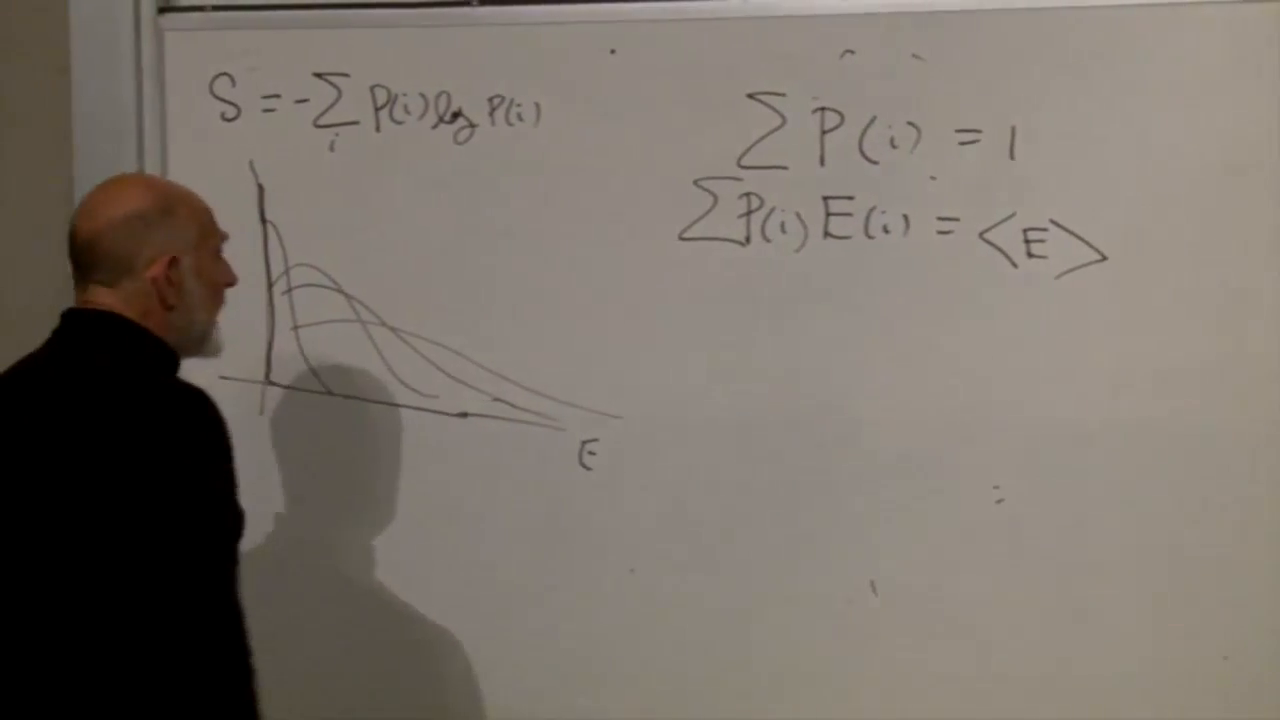
\includegraphics[width=0.88\textwidth]{lecture_03_figure_02.png}
\caption{Le tableau d’ouverture rassemble les formules de l’entropie, de la normalisation et de l’énergie moyenne, ainsi qu’une famille qualitative de distributions d’équilibre.}
\lectureframe{00:06:44}
\end{figure}

\section{L’équilibre comme famille de distributions}

Le cours précédent nous a laissé une famille de distributions d’équilibre à un paramètre. On peut paramétrer cette famille par la température, mais, pour l’instant, il est plus utile de la paramétrer par l’énergie moyenne \(\overline E\). À l’énergie minimale possible, la distribution est concentrée sur un état fondamental :
\[
 P_i=\delta_{i0}.
\]
L’état est alors connu sans incertitude, et \(S=0\). À mesure que la distribution d’équilibre s’étend à davantage de niveaux d’énergie, son énergie moyenne et son entropie augmentent toutes deux.

Il s’agit d’une propriété de la famille thermique, et non de toute distribution que l’on pourrait imaginer. Une famille arbitraire pourrait se déplacer vers des énergies plus élevées tout en se resserrant. Les distributions d’équilibre que nous allons déduire ne se comportent pas ainsi dans le régime usuel de température positive. Le long de cette famille,
\begin{equation}
 \frac{dS}{d\overline E}>0.
 \label{eq:sm3-positive-temperature-branch}
\end{equation}
Les systèmes dont le spectre est borné peuvent aussi présenter des branches où cette dérivée est négative. Ces régimes de température négative existent bel et bien, mais nous les laissons de côté dans le présent raisonnement.

L’équilibre thermique ne signifie pas que les mouvements microscopiques cessent. Les molécules continuent de se déplacer, d’entrer en collision et d’échanger de l’énergie. C’est la description macroscopique qui devient stationnaire : la distribution ne présente plus de dérive nette, et les différentes parties du système ne sont plus parcourues par un flux net d’énergie.

\section{Les lois de la thermodynamique dans le langage statistique}

Le premier principe exprime la conservation de l’énergie. Le deuxième principe stipule que l’entropie thermodynamique d’un système macroscopique isolé ne diminue pas :
\begin{equation}
 \Delta S_{\mathrm{tot}}\geq0.
 \label{eq:sm3-second-law}
\end{equation}
Une égalité correspond à l’équilibre ou à une transformation idéale réversible ; une relaxation spontanée entraîne généralement une augmentation stricte.

Dans la description probabiliste, la relaxation tend à répartir le poids entre les possibilités macroscopiques que nous distinguons encore. Il faut assortir cette affirmation de la réserve soulignée pendant le cours : nous effectuons un \emph{regroupement grossier}. L’évolution hamiltonienne exacte conserve l’entropie fine dans l’espace des phases. L’entropie macroscopique augmente parce que nous cessons de suivre les corrélations et les détails microscopiques. La perte de ces informations élargit la description réduite. Un resserrement spontané signifierait au contraire que nous avons acquis des informations microscopiques sans effectuer de mesure.

Le principe zéro affirme que les systèmes peuvent atteindre l’équilibre thermique et que cette relation d’équilibre est transitive. Si \(A\) est en équilibre avec \(B\), et \(B\) avec \(C\), alors \(A\) est en équilibre avec \(C\). La température est la grandeur qui rend cette transitivité manifeste :
\[
 T_A=T_B,\qquad T_B=T_C
 \quad\Longrightarrow\quad
 T_A=T_C.
\]
Hors équilibre, l’énergie passe du sous-système dont la température est la plus élevée vers celui dont la température est la plus basse. À températures égales, le flux net cesse. Nous allons maintenant déduire cette affirmation opérationnelle de la définition de la température par l’entropie.

\section{Pourquoi l’énergie passe du chaud vers le froid}

Considérons deux sous-systèmes faiblement couplés, \(A\) et \(B\). Chacun est en équilibre interne, mais leurs températures diffèrent. Choisissons les indices de sorte que
\begin{equation}
 T_B>T_A>0.
 \label{eq:sm3-temperature-order}
\end{equation}
Lors d’un petit échange, la conservation de l’énergie totale donne
\begin{equation}
 dE_A+dE_B=0.
 \label{eq:sm3-energy-conservation}
\end{equation}
Le deuxième principe donne
\begin{equation}
 dS_A+dS_B\geq0.
 \label{eq:sm3-entropy-change}
\end{equation}
Pour chaque sous-système en équilibre interne, la température est définie par
\begin{equation}
 dE_X=T_X\,dS_X,
 \qquad X=A,B.
 \label{eq:sm3-temperature-differential}
\end{equation}
En substituant dans \eqref{eq:sm3-energy-conservation}, on obtient
\begin{equation}
 T_A\,dS_A+T_B\,dS_B=0,
\end{equation}
d’où
\begin{equation}
 dS_B=-\frac{T_A}{T_B}\,dS_A.
 \label{eq:sm3-dsb}
\end{equation}
En reportant ce résultat dans \eqref{eq:sm3-entropy-change},
\begin{align}
 dS_{\mathrm{tot}}
 &=dS_A-\frac{T_A}{T_B}dS_A\\
 &=\frac{T_B-T_A}{T_B}\,dS_A\geq0.
 \label{eq:sm3-flow-entropy}
\end{align}
Comme \(T_B-T_A>0\) et \(T_B>0\), un échange spontané exige
\[
 dS_A>0.
\]
L’équation \eqref{eq:sm3-temperature-differential} donne alors
\begin{equation}
 dE_A=T_A\,dS_A>0,
 \qquad
 dE_B=-dE_A<0.
 \label{eq:sm3-hot-to-cold}
\end{equation}
L’énergie est passée de \(B\), le sous-système le plus chaud, à \(A\), le plus froid. Ici, la chaleur désigne simplement l’énergie en transit. Le flux se poursuit jusqu’à ce que \(T_A=T_B\), lorsque la variation d’entropie au premier ordre ne favorise plus aucune direction.

On peut présenter le même résultat en une seule ligne :
\begin{equation}
 dS_{\mathrm{tot}}
 =dE_A\left(\frac{1}{T_A}-\frac{1}{T_B}\right)\geq0.
 \label{eq:sm3-compact-flow}
\end{equation}
Le signe de la différence des inverses des températures détermine le signe de \(dE_A\). Cette forme compacte s’accordera naturellement plus tard avec l’ensemble canonique.

\begin{classroomqa}
\audiencequestion{Ce raisonnement suppose-t-il que \(A\) et \(B\) sont déjà chacun en équilibre interne ?}
\lecturerresponse{Oui. Attribuer une seule valeur de \(T_A\) ou de \(T_B\) suppose cet équilibre. Si un sous-système n’est pas en équilibre interne, on le divise en régions plus petites et on applique localement le raisonnement partout où l’on peut définir une température. La relaxation globale résulte alors des échanges entre ces régions.
\lecturetimestamp{00:24:38--00:25:22}}
\end{classroomqa}

\section{Qu’entend-on par état ?}

Avant de chercher les probabilités d’équilibre, nous devons savoir ce que désigne l’indice \(i\). Un état microscopique est la description la plus complète du système que permettent les lois physiques sous-jacentes. En mécanique classique, on se représente les positions et les moments de toutes les particules. En mécanique quantique, un état est plutôt un état quantique complet ; le principe d’incertitude interdit de spécifier simultanément avec une précision arbitraire toutes les positions et tous les moments classiques.

Pour un système quantique dans une boîte finie, le dénombrement pertinent des états peut être discret. La mécanique statistique classique émerge dans une limite appropriée, où les sommes sur des états quantiques très rapprochés deviennent des intégrales dans l’espace des phases. Cette limite introduit aussi la cellule d’espace des phases nécessaire pour rendre l’entropie continue sans dimension ; elle ne s’obtient pas en remplaçant simplement un signe de sommation par un signe intégral.

\begin{classroomqa}
\audiencequestion{Pour un gaz, faut-il se représenter un état comme les positions et les moments de chaque molécule ?}
\lecturerresponse{C’est bien la représentation classique. Plus généralement, un état désigne tout ce qui pourrait en principe être connu du système, dans les limites imposées par les lois physiques. La mécanique quantique modifie la forme de cette description maximale et rend discret le dénombrement dans un volume fini. Retrouver l’intégrale classique à partir de la somme quantique exige une véritable démarche de passage à la limite ; ce n’est pas une substitution en une ligne.
\lecturetimestamp{00:25:31--00:27:38}}
\end{classroomqa}

\section{Un bain thermique constitué de répliques}

La question difficile se pose désormais inévitablement : une fois l’équilibre établi, qu’est-ce qui détermine \(P_i\) ?

Mettons le sous-système en contact avec un bain thermique de très grande taille. L’énergie peut passer dans les deux sens, mais le bain possède tellement de degrés de liberté qu’un petit transfert d’énergie modifie à peine sa température. Un bain particulièrement commode est constitué de nombreuses répliques du sous-système lui-même, faiblement couplées entre elles. Une réplique est le système étudié ; les autres constituent son environnement.

Cette construction correspond souvent à un véritable système macroscopique. Divisons un grand corps presque homogène en cellules semblables. Chaque cellule est un sous-système, et les autres cellules forment son bain. Notons \(N\) le nombre total de répliques. La démonstration en classe utilise neuf répliques et trois étiquettes d’état colorées, mais le dénombrement ne dépend pas de ces nombres particuliers.

Soit \(n_i\) le nombre de répliques dans l’état \(i\). Ce sont les \emph{nombres d’occupation}. Il peut exister une infinité de niveaux d’énergie, mais, à énergie totale finie, l’occupation de la plupart des niveaux très élevés est négligeable ou nulle.

La première contrainte porte simplement sur le nombre de répliques :
\begin{equation}
 \sum_i n_i=N.
 \label{eq:sm3-number-constraint}
\end{equation}
La seconde porte sur l’énergie totale :
\begin{equation}
 \sum_i n_iE_i=N\overline E.
 \label{eq:sm3-total-energy-constraint}
\end{equation}
Le membre de droite est une grandeur extensive. Si l’on double le nombre de répliques tout en maintenant leur état statistique, l’énergie totale double, tandis que l’énergie moyenne par réplique reste égale à \(\overline E\).

\begin{classroomqa}
\audiencequestion{La construction avec des répliques doit-elle aussi satisfaire une contrainte sur l’énergie ?}
\lecturerresponse{Oui. La somme des nombres d’occupation doit être égale à \(N\), et leur somme pondérée par l’énergie doit être égale à l’énergie totale fixée \(N\overline E\). Ce sont précisément les deux contraintes qui limiteront ensuite la maximisation de l’entropie.
\lecturetimestamp{00:37:12--00:39:54}}
\end{classroomqa}

La probabilité qu’une réplique choisie au hasard soit dans l’état \(i\) est sa fréquence relative :
\begin{equation}
 P_i=\frac{n_i}{N},
 \qquad
 n_i=NP_i.
 \label{eq:sm3-frequency-probability}
\end{equation}

\begin{figure}[t]
\centering
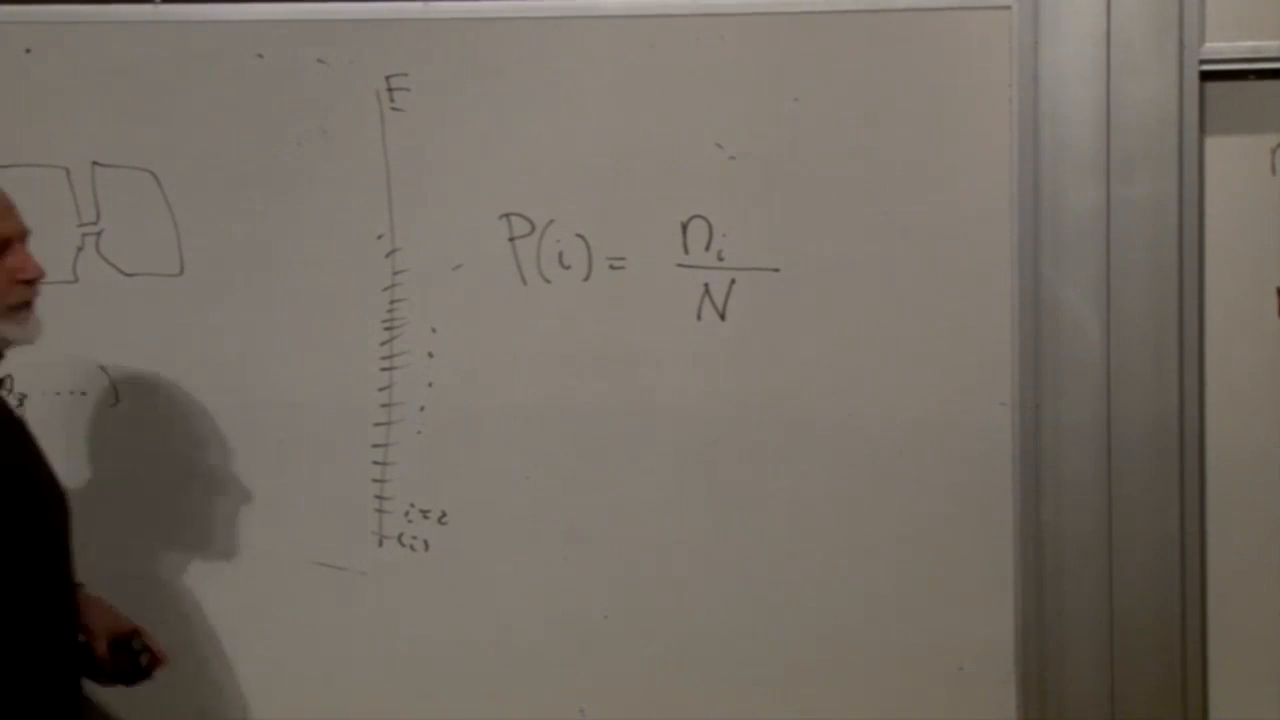
\includegraphics[width=0.82\textwidth]{lecture_03_figure_03.png}
\caption{Le schéma des niveaux d’énergie et l’identification de la probabilité à la fraction d’occupation \(P_i=n_i/N\).}
\lectureframe{00:41:40}
\end{figure}

\begin{classroomqa}
\audiencequestion{La notation \(N(i)\) au tableau est-elle censée différer de \(n_i\) ?}
\lecturerresponse{Non. Les deux désignent le nombre d’occupation de l’état \(i\). Nous utilisons systématiquement \(n_i\) et réservons la lettre majuscule \(N\) au nombre total de répliques.
\lecturetimestamp{00:41:28--00:41:33}}
\end{classroomqa}

En divisant \eqref{eq:sm3-number-constraint} et \eqref{eq:sm3-total-energy-constraint} par \(N\), on retrouve les contraintes sur les probabilités :
\begin{equation}
 \sum_iP_i=1,
 \qquad
 \sum_iP_iE_i=\overline E.
 \label{eq:sm3-probability-constraints}
\end{equation}
L’interprétation des fréquences dans l’ensemble a donc redonné les équations par lesquelles nous avons commencé.

\section{Multiplicité d’une configuration d’occupation}

Fixons un ensemble de nombres d’occupation \(\{n_i\}\). Combien d’affectations des \(N\) répliques discernables aux états réalisent exactement cet ensemble ? La réponse est le coefficient multinomial
\begin{equation}
 C(\{n_i\})=\frac{N!}{\prod_i n_i!}.
 \label{eq:sm3-multiplicity}
\end{equation}
Pour comprendre le dénominateur, commençons par ranger les \(N\) répliques étiquetées de \(N!\) façons. Permuter les \(n_i\) répliques qui occupent le même état ne produit pas une nouvelle affectation des occupations ; on divise donc par \(n_i!\) pour chaque état.

\begin{figure}[t]
\centering
\includegraphics[width=0.88\textwidth]{lecture_03_figure_04.png}
\caption{La multiplicité multinomiale
\(C=N!/\prod_i n_i!\) inscrite au tableau.}
\lectureframe{00:46:55}
\end{figure}

Les niveaux inoccupés ne posent aucun problème, car \(0!=1\). Si toutes les répliques occupent un même état, alors
\[
 C=\frac{N!}{N!}=1,
\]
comme prévu. Si trois répliques occupent trois états spécifiés distincts, alors
\[
 C=\frac{3!}{1!\,1!\,1!}=6.
\]
Avec deux répliques occupant deux états spécifiés, la formule donne deux affectations : on échange l’état occupé par chacune des répliques étiquetées.

\begin{classroomqa}
\audiencequestion{Plusieurs ensembles de nombres d’occupation peuvent-ils satisfaire les deux contraintes ?}
\lecturerresponse{En général, oui, il en existe beaucoup. L’équation \eqref{eq:sm3-multiplicity} compte d’abord les arrangements correspondant à un ensemble fixé \(\{n_i\}\), sans décider encore s’il satisfait les contraintes. À l’étape suivante, on compare tous les ensembles compatibles avec les contraintes pour déterminer lequel a la plus grande multiplicité.
\lecturetimestamp{00:48:07--00:48:43}}
\end{classroomqa}

L’hypothèse statistique consiste à traiter de façon symétrique les affectations microscopiques compatibles avec le système isolé. Une configuration macroscopique d’occupation réalisée par un plus grand nombre d’affectations est donc plus probable. Pour un grand \(N\), la distribution des fractions \(n_i/N\) présente un pic très marqué. Les fractions d’équilibre sont les valeurs qui maximisent \(C\) sous les contraintes \eqref{eq:sm3-number-constraint} et \eqref{eq:sm3-total-energy-constraint}.

\section{L’approximation de Stirling}

Les factorielles deviennent énormes bien avant que \(N\) n’atteigne une valeur macroscopique ; nous travaillons donc avec leurs logarithmes. Partons de
\begin{equation}
 \log N!=\sum_{x=1}^{N}\log x.
 \label{eq:sm3-log-factorial-sum}
\end{equation}
Pour un grand \(N\), la somme est approchée par l’aire sous \(\log x\) :
\begin{align}
 \log N!
 &\simeq\int_1^N\log x\,dx\\
 &=\left[x\log x-x\right]_1^N\\
 &=N\log N-N+1.
 \label{eq:sm3-stirling-integral}
\end{align}
La primitive se déduit immédiatement de
\[
 \frac{d}{dx}(x\log x-x)=\log x.
\]
Au premier ordre extensif, on peut négliger la constante additive :
\begin{equation}
 \log N!\simeq N\log N-N.
 \label{eq:sm3-stirling-log}
\end{equation}
En prenant l’exponentielle, on obtient la forme simplifiée utilisée dans le cours,
\begin{equation}
 N!\simeq N^N e^{-N}.
 \label{eq:sm3-stirling-simple}
\end{equation}

\begin{figure}[t]
\centering
\includegraphics[width=0.88\textwidth]{lecture_03_figure_05.png}
\caption{L’approximation de Stirling au premier ordre et sa dérivation, qui remplace la somme de \(\log x\) par une intégrale.}
\lectureframe{01:03:45}
\end{figure}

\begin{classroomqa}
\audiencequestion{L’évaluation de \(x\log x-x\) à la borne inférieure laisse-t-elle un terme supplémentaire \(+1\) ?}
\lecturerresponse{Oui. L’équation \eqref{eq:sm3-stirling-integral} contient cette constante. Elle est négligeable devant les termes proportionnels à \(N\) lorsque \(N\to\infty\), ce qui explique son omission dans la formule au premier ordre. La somme doit commencer à \(x=1\) ; \(\log0\) n’est pas défini.
\lecturetimestamp{01:04:12--01:04:35}}
\end{classroomqa}

\begin{classroomqa}
\audiencequestion{Un facteur proportionnel à \(\sqrt{N}\) manque-t-il aussi ?}
\lecturerresponse{Oui. La formule asymptotique plus précise est
\[
 N!\sim\sqrt{2\pi N}\left(\frac{N}{e}\right)^N.
\]
Son logarithme n’apporte qu’une contribution de \(\tfrac12\log(2\pi N)\), sous-extensive
par rapport à \(N\log N-N\). Elle importe pour calculer avec précision les
probabilités à \(N\) fini, mais pas pour le calcul de l’entropie au premier ordre d’un système macroscopique.
\lecturetimestamp{01:04:35--01:05:40}}
\end{classroomqa}

Il faut également appliquer avec précaution l’approximation de Stirling au dénominateur de \eqref{eq:sm3-multiplicity}. À la limite thermodynamique, les états dont les probabilités limites sont non nulles vérifient \(n_i=NP_i\) ; leurs occupations croissent donc avec \(N\). On peut traiter les états dont l’occupation est très faible ou nulle au moyen d’une coupure en énergie finie, puis rétablir la limite. Les termes sous-dominants omis ne modifient pas l’entropie extensive au premier ordre.

\section{Le logarithme de la multiplicité est l’entropie}

Appliquons \eqref{eq:sm3-stirling-simple} au numérateur et à tous les facteurs du dénominateur correspondant à des occupations macroscopiques :
\begin{equation}
 C\simeq
 \frac{N^Ne^{-N}}
 {\prod_i n_i^{\,n_i}e^{-n_i}}.
 \label{eq:sm3-c-stirling}
\end{equation}
Puisque \(\sum_i n_i=N\), les facteurs exponentiels dominants se simplifient :
\begin{equation}
 C\simeq\frac{N^N}{\prod_i n_i^{\,n_i}}.
 \label{eq:sm3-c-leading}
\end{equation}
Il est plus facile de maximiser un logarithme qu’un produit, et le logarithme étant une fonction croissante, les deux maxima correspondent à la même configuration d’occupation :
\begin{equation}
 \log C=N\log N-\sum_i n_i\log n_i.
 \label{eq:sm3-logc-occupations}
\end{equation}
Substituons maintenant \(n_i=NP_i\) :
\begin{align}
 \log C
 &=N\log N-\sum_iNP_i\log(NP_i)\\
 &=N\log N-N\sum_iP_i\log N
   -N\sum_iP_i\log P_i\\
 &=-N\sum_iP_i\log P_i,
 \label{eq:sm3-logc-entropy-derivation}
\end{align}
où la normalisation annule les deux termes \(N\log N\). Ainsi, au premier ordre en \(N\),
\begin{equation}
 \boxed{\log C=NS}.
 \label{eq:sm3-logc-ns}
\end{equation}

\begin{figure}[t]
\centering
\includegraphics[width=0.88\textwidth]{lecture_03_figure_06.png}
\caption{Le calcul au tableau qui relie
\(\log C=N\log N-\sum_i n_i\log n_i\) à
\(-N\sum_iP_i\log P_i=NS\).}
\lectureframe{01:16:10}
\end{figure}

Cette relation est au cœur du chapitre. L’entropie n’est pas une grandeur sans lien avec le problème de dénombrement. Elle représente la multiplicité par réplique, mesurée logarithmiquement. Maximiser le nombre d’arrangements microscopiques revient donc, au premier ordre, à maximiser l’entropie d’une réplique.

\begin{classroomqa}
\audiencequestion{La multiplicité ne serait-elle pas maximale lorsque tous les nombres d’occupation sont égaux ?}
\lecturerresponse{La répartition est uniforme lorsqu’aucun état n’est privilégié et que seule la contrainte \(\sum_i n_i=N\) s’applique sur un ensemble fini d’états. La contrainte d’énergie fixée modifie la réponse, car les valeurs \(E_i\) diffèrent. Des occupations égales ne donnent généralement pas l’énergie moyenne spécifiée.
\lecturetimestamp{01:17:07--01:18:20}}
\end{classroomqa}

\begin{classroomqa}
\audiencequestion{La lettre majuscule \(N\) désigne un grand nombre, mais pourquoi peut-on appliquer l’approximation de Stirling à chaque \(n_i\) du dénominateur ?}
\lecturerresponse{Pour chaque état dont la probabilité limite est non nulle, \(n_i=NP_i\) croît proportionnellement à \(N\). On peut d’abord conserver un intervalle d’énergie fini, prendre la limite de grand \(N\) sur cet intervalle, puis l’élargir. Les états clairsemés de la queue exigent des corrections finies distinctes, mais ils ne modifient pas l’entropie extensive au premier ordre.
\lecturetimestamp{01:18:23--01:19:28}}
\end{classroomqa}

\begin{classroomqa}
\audiencequestion{Cette approximation pour grand \(N\) correspond-elle à ce qu’on appelait plus tôt le regroupement grossier ?}
\lecturerresponse{Non. La limite thermodynamique porte sur les grands nombres d’occupation et le dénombrement asymptotique. Le regroupement grossier consiste à perdre ou à écarter délibérément la résolution microscopique. Ce sont deux opérations distinctes, même si elles sont toutes deux souvent utilisées en mécanique statistique macroscopique.
\lecturetimestamp{01:19:29--01:19:46}}
\end{classroomqa}

\begin{classroomqa}
\audiencequestion{Puisque
\(\log C=N\log N-\sum_i n_i\log n_i\), faut-il minimiser le second terme plutôt que le maximiser ?}
\lecturerresponse{Oui ; à \(N\) fixé, maximiser \(\log C\) revient à minimiser \(\sum_i n_i\log n_i\). Après substitution de \(n_i=NP_i\), les termes fixes en \(N\log N\) se simplifient et il reste \(-N\sum_iP_i\log P_i=NS\). Il est donc plus naturel de décrire cette même opération comme la maximisation de l’entropie positive \(S\).
\lecturetimestamp{01:19:48--01:20:55}}
\end{classroomqa}

\begin{classroomqa}
\audiencequestion{Pourquoi ne pas conclure immédiatement le raisonnement par symétrie et poser tous les \(n_i\) égaux ?}
\lecturerresponse{Ce raccourci néglige les étiquettes d’énergie. La contrainte de normalisation traite les états de façon symétrique, mais ce n’est pas le cas de \(\sum_iP_iE_i=\overline E\) : des états d’énergies différentes contribuent différemment. C’est précisément la contrainte d’énergie qui fait apparaître la distribution d’équilibre non uniforme.
\lecturetimestamp{01:21:15--01:21:41}}
\end{classroomqa}

\section{Le problème de maximisation de l’entropie}

Nous pouvons maintenant énoncer sans ambiguïté la règle de mécanique statistique. Faisons varier les probabilités \(P_i\) et maximisons
\begin{equation}
 S[P]=-\sum_iP_i\log P_i
 \label{eq:sm3-maximize-entropy}
\end{equation}
sous les contraintes
\begin{equation}
 \sum_iP_i=1,
 \qquad
 \sum_iP_iE_i=\overline E.
 \label{eq:sm3-maxent-constraints}
\end{equation}
Les probabilités maximisantes donnent les fractions d’occupation nettement privilégiées dans un grand ensemble de répliques. Les nombres d’occupation fluctuent, mais leurs écarts relatifs diminuent lorsque \(N\) augmente, si bien que les rapports \(n_i/N\) deviennent des probabilités thermodynamiques bien définies.

\begin{classroomqa}
\audiencequestion{Les \(E_i\) sont-elles les énergies fixes des états, tandis que la contrainte fait intervenir une énergie totale donnée séparément ?}
\lecturerresponse{Oui. Le spectre \(\{E_i\}\) appartient au sous-système. L’énergie totale de l’ensemble complet de répliques est fixée, mais l’énergie circule continuellement entre les répliques. Diviser cette énergie totale par \(N\) fixe l’énergie moyenne \(\overline E\) d’une réplique, et non son énergie dans chaque réalisation microscopique.
\lecturetimestamp{01:26:12--01:27:07}}
\end{classroomqa}

Le problème est facile à énoncer, mais il n’est pas encore résolu. Il s’agit d’une optimisation sous deux contraintes ; il nous faut donc un outil mathématique supplémentaire.

\section{Les multiplicateurs de Lagrange}

Pour une fonction non contrainte \(F(x_1,x_2,\ldots)\), un point stationnaire vérifie
\begin{equation}
 \frac{\partial F}{\partial x_i}=0
 \qquad\text{for every }i.
 \label{eq:sm3-unconstrained-stationary}
\end{equation}
Imposons maintenant en plus que
\begin{equation}
 G(x_1,x_2,\ldots)=0.
 \label{eq:sm3-one-constraint}
\end{equation}

\begin{classroomqa}
\audiencequestion{Que signifie \(x\) si la figure comporte les coordonnées \(x\) et \(y\) ?}
\lecturerresponse{Ici, \(x\) est une abréviation pour le vecteur de coordonnées complet \((x_1,x_2,\ldots)\). Dans le dessin à deux dimensions, ses composantes sont simplement \(x\) et \(y\). Plus tard, les composantes seront les probabilités \(P_1,P_2,\ldots\).
\lecturetimestamp{01:30:12--01:30:20}}
\end{classroomqa}

Géométriquement, les courbes de niveau \(F=\text{constant}\) forment une carte de contours, tandis que \(G=0\) est la courbe sur laquelle le système est contraint de se déplacer. Un extremum sous contrainte se produit lorsqu’une courbe de niveau de \(F\) est tangente à la courbe de contrainte. En ce point, les gradients sont parallèles :
\begin{equation}
 \nabla F=-\lambda\nabla G
 \label{eq:sm3-parallel-gradients}
\end{equation}
pour un certain nombre \(\lambda\).

\begin{figure}[t]
\centering
\includegraphics[width=0.88\textwidth]{lecture_03_figure_07.png}
\caption{La géométrie des courbes de niveau au tableau et la fonction augmentée \(F'=F+\lambda G\). Un extremum sous contrainte se trouve au point de tangence.}
\lectureframe{01:37:10}
\end{figure}

On peut obtenir l’équation \eqref{eq:sm3-parallel-gradients} en définissant la fonction augmentée
\begin{equation}
 F'=F+\lambda G
 \label{eq:sm3-augmented-function}
\end{equation}
et en imposant la condition de stationnarité ordinaire :
\begin{equation}
 \frac{\partial F'}{\partial x_i}=0.
 \label{eq:sm3-augmented-stationarity}
\end{equation}
Le multiplicateur \(\lambda\) est inconnu au départ. Cela ne rend pas le système sous-déterminé, puisque la contrainte initiale \(G=0\) fournit une équation supplémentaire.

\begin{classroomqa}
\classquestion{Pourquoi l’ajout d’un terme proportionnel à \(G\) rend-il le point sous contrainte stationnaire ?}
\lecturerresponse{À l’extremum sous contrainte, un déplacement tangent à \(G=0\) ne produit déjà aucune variation au premier ordre de \(F\). La seule pente restante est normale à la contrainte. Comme \(\nabla G\) pointe dans cette même direction normale, un choix approprié de \(\lambda\) l’annule :
\(\nabla F+\lambda\nabla G=0\).
\lecturetimestamp{01:35:06--01:35:32}}
\end{classroomqa}

\section{Un exemple à deux variables}

Minimisons
\begin{equation}
 F(x,y)=\frac{x^2+y^2}{2}
 \label{eq:sm3-example-f}
\end{equation}
sous la contrainte
\begin{equation}
 x+y=1.
 \label{eq:sm3-example-constraint}
\end{equation}
Écrivons la contrainte sous la forme \(G=x+y-1=0\) et construisons
\begin{equation}
 F'=\frac{x^2+y^2}{2}+\lambda(x+y-1).
 \label{eq:sm3-example-augmented}
\end{equation}
Les équations stationnaires sont
\begin{align}
 \frac{\partial F'}{\partial x}&=x+\lambda=0,\\
 \frac{\partial F'}{\partial y}&=y+\lambda=0.
 \label{eq:sm3-example-derivatives}
\end{align}
Ainsi, \(x=y=-\lambda\). L’équation restante est la contrainte,
\[
 x+y=-2\lambda=1,
\]
d’où
\begin{equation}
 \lambda=-\frac12,
 \qquad
 x=y=\frac12.
 \label{eq:sm3-example-solution}
\end{equation}
Le point \((1/2,1/2)\) est celui où le plus petit cercle centré à l’origine est tangent à la droite \(x+y=1\).

\begin{figure}[t]
\centering
\includegraphics[width=0.88\textwidth]{lecture_03_figure_08.png}
\caption{Le calcul complet par multiplicateurs de Lagrange pour minimiser \((x^2+y^2)/2\) sous la contrainte \(x+y=1\).}
\lectureframe{01:44:10}
\end{figure}

Avec plusieurs contraintes, introduisons un multiplicateur pour chacune :
\begin{equation}
 F'=F+\lambda_1G_1+\lambda_2G_2+\cdots.
 \label{eq:sm3-many-multipliers}
\end{equation}
Résolvons ensuite
\begin{equation}
 \begin{aligned}
 \frac{\partial F'}{\partial x_i}&=0
 &&\text{for every }i,\\
 G_a&=0
 &&\text{for every constraint }a.
 \end{aligned}
 \label{eq:sm3-many-equations}
\end{equation}
Le cours propose un exercice d’entraînement volontairement artificiel : optimiser une fonction quadratique de \(x,y,z\) en imposant deux contraintes linéaires indépendantes, telles que \(x+y=1\) et \(z+x=1\). L’intérêt ne tient pas à la réponse particulière, mais à la règle selon laquelle chaque contrainte apporte à la fois un multiplicateur et une équation.

\section{Le problème en vue du cours suivant}

En mécanique statistique, les coordonnées sont les probabilités \(\{P_i\}\), la fonction à maximiser est l’entropie, et les contraintes sont la normalisation et la valeur fixée de l’énergie moyenne. Définissons
\begin{align}
 S[P]&=-\sum_iP_i\log P_i,\\
 G_1[P]&=\sum_iP_i-1,\\
 G_2[P]&=\sum_iP_iE_i-\overline E.
 \label{eq:sm3-final-functions}
\end{align}
L’entropie augmentée peut donc s’écrire
\begin{equation}
 \Phi[P]
 =S[P]+\alpha G_1[P]+\beta G_2[P].
 \label{eq:sm3-final-augmented}
\end{equation}
Les équations à résoudre sont
\begin{equation}
 \frac{\partial\Phi}{\partial P_i}=0
 \quad\text{for every }i,
 \qquad
 G_1=0,
 \qquad
 G_2=0.
 \label{eq:sm3-final-problem}
\end{equation}

\begin{figure}[H]
\centering
\includegraphics[width=0.88\textwidth]{lecture_03_figure_09.png}
\caption{Le tableau de clôture : l’entropie en fonction des probabilités, avec la normalisation et la valeur fixée de l’énergie moyenne.}
\lectureframe{01:53:05}
\end{figure}

À ce stade, le problème est entièrement posé. La résolution de \eqref{eq:sm3-final-problem} donne la distribution d’équilibre. Le multiplicateur associé à l’énergie deviendra l’inverse de la température, \(\beta=1/T\), selon la convention de signe choisie dans \eqref{eq:sm3-final-augmented}. Le cours suivant effectuera cette dérivation et obtiendra les poids de Boltzmann.
\chapter{Poids de Boltzmann, fonctions de partition et gaz parfait}

\lectureoverview{Nous déduisons la distribution de probabilité à l’équilibre en maximisant l’entropie sous les contraintes de normalisation et d’énergie moyenne fixée. La fonction de partition permet ensuite d’obtenir l’énergie moyenne, l’entropie et la température par dérivation. Le gaz parfait en fournit le premier exemple complet, suivi d’une extension gravitationnelle et d’un aperçu des fluctuations d’énergie.}

\section{Le problème d’entropie sous contraintes}

Considérons un grand ensemble de \(\mathcal N\) répliques identiques, interagissant très faiblement, d’un même sous-système. Si \(n_i\) répliques occupent le \(i\)-ième état, alors
\begin{equation}
 p_i=\frac{n_i}{\mathcal N},
 \qquad
 \sum_i p_i=1.
 \label{eq:sm4-occupation-probability}
\end{equation}
Le dénombrement multinomial du cours précédent donne l’entropie par réplique,
\begin{equation}
 S[p]=-\sum_i p_i\log p_i.
 \label{eq:sm4-entropy}
\end{equation}
Il est utile de considérer cette expression comme une fonction ordinaire de toutes les variables \(p_1,p_2,\ldots\). Sa forme additive simple rend le calcul possible.

L’énergie totale de l’ensemble de répliques est fixée à \(\mathcal N E\), où \(E\) désigne l’énergie moyenne par réplique. La seconde contrainte est donc
\begin{equation}
 \sum_i p_iE_i=E.
 \label{eq:sm4-energy-constraint}
\end{equation}
Les niveaux \(E_i\) appartiennent au sous-système ; le nombre \(E\) au membre de droite est leur moyenne pondérée par les probabilités. La maximisation de \eqref{eq:sm4-entropy} sous les contraintes \eqref{eq:sm4-occupation-probability} et \eqref{eq:sm4-energy-constraint} sélectionne les fractions d’occupation de très loin les plus probables.

Pour simplifier, minimisons \(-S=\sum_i p_i\log p_i\). Introduisons un multiplicateur de Lagrange pour chaque contrainte :
\begin{equation}
 \begin{aligned}
 \Phi[p;\alpha,\beta]
 &=\sum_i p_i\log p_i\\
 &\quad+\alpha\left(\sum_i p_i-1\right)\\
 &\quad+\beta\left(\sum_i p_iE_i-E\right).
 \end{aligned}
 \label{eq:sm4-augmented-functional}
\end{equation}
Les noms \(\alpha\) et \(\beta\) ne correspondent pas encore à des hypothèses physiques. À ce stade, ce sont simplement les deux nombres nécessaires pour imposer les deux contraintes.

\begin{classroomqa}
\audiencequestion{La fonction augmentée dépend-elle aussi de \(\alpha\) et de \(\beta\) ?}
\lecturerresponse{Oui. La variation par rapport à \(\alpha\) et \(\beta\) rétablit les deux contraintes. Pour le calcul immédiat, toutefois, nous maintenons ces multiplicateurs fixes et faisons varier les probabilités \(p_i\). Leurs valeurs seront déterminées ensuite par la normalisation et l’énergie moyenne prescrite.
\lecturetimestamp{00:09:32--00:09:49}}
\end{classroomqa}

\begin{figure}[t]
\centering
\includegraphics[width=0.92\textwidth]{lecture_04_figure_02.png}
\caption{La fonctionnelle d’entropie augmentée, après suppression des termes constants lors de la variation des probabilités.}
\lectureframe{00:10:56}
\end{figure}

Lorsqu’on dérive par rapport à une probabilité, les termes \(-\alpha\) et \(-\beta E\) ne contribuent pas. C’est la fonctionnelle abrégée que l’on voit au tableau. Ils font toujours partie de \eqref{eq:sm4-augmented-functional} ; ils sont simplement sans effet sur cette dérivée particulière.

\section{La distribution de Boltzmann}

Choisissons une probabilité quelconque. Le cours choisit \(p_7\), en partie parce que \(1\) paraît trop particulier et que \(7\) est un chiffre porte-bonheur. Ce choix n’a aucune incidence. Le seul calcul différentiel nécessaire est
\begin{equation}
 \frac{d}{dp_i}\bigl(p_i\log p_i\bigr)=\log p_i+1.
\end{equation}
On obtient donc
\begin{equation}
 \frac{\partial\Phi}{\partial p_i}
 =\log p_i+1+\alpha+\beta E_i=0.
 \label{eq:sm4-stationarity}
\end{equation}
En isolant \(p_i\),
\begin{align}
 \log p_i&=-(1+\alpha)-\beta E_i,\\
 p_i&=e^{-(1+\alpha)}e^{-\beta E_i}.
\end{align}
Le premier facteur est indépendant de l’indice d’état. Notons-le \(1/Z\) :
\begin{equation}
 p_i=\frac{e^{-\beta E_i}}{Z}.
 \label{eq:sm4-boltzmann-weight}
\end{equation}

C’est le premier résultat immédiat. Une dérivée sous contrainte tout à fait ordinaire a produit une loi exponentielle. Les probabilités relatives vérifient
\begin{equation}
 \frac{p_i}{p_j}=e^{-\beta(E_i-E_j)}.
 \label{eq:sm4-relative-weight}
\end{equation}
Le multiplicateur \(\beta\) détermine la rapidité avec laquelle la probabilité décroît en fonction de l’énergie. Une grande valeur positive de \(\beta\) concentre la distribution près des niveaux les plus bas ; une petite valeur positive de \(\beta\) répartit un poids appréciable plus haut dans le spectre. On voit déjà que la variation de \(\beta\) modifie l’énergie moyenne, même s’il reste à démontrer que ce paramètre s’identifie à l’inverse de la température.

\section{Normalisation et fonction de partition}

La normalisation détermine le facteur indépendant de l’état :
\begin{equation}
 1=\sum_i p_i
 =\frac{1}{Z}\sum_i e^{-\beta E_i},
\end{equation}
d’où
\begin{equation}
 Z(\beta)=\sum_i e^{-\beta E_i}.
 \label{eq:sm4-partition-function}
\end{equation}
C’est la fonction de partition canonique. Elle est d’abord apparue comme une constante de normalisation, mais ce rôle est loin de rendre compte de toute son importance. Une fois \(Z(\beta)\) connue, on obtient les grandeurs thermodynamiques à partir de ses dérivées.

Les niveaux d’énergie qui figurent dans \eqref{eq:sm4-partition-function} sont des données d’entrée. Ils découlent de la mécanique du système et des conditions extérieures fixées : le volume et la forme de la boîte, les champs magnétiques ou électriques, ainsi que tout autre paramètre de contrôle. La variation d’un paramètre de contrôle modifie le spectre et, par conséquent, \(Z\). Dans le calcul présent, ces paramètres, et donc l’ensemble \(\{E_i\}\), sont maintenus fixes.

\begin{classroomqa}
\audiencequestion{Que représentent exactement les axes du schéma de la fonction exponentielle ? L’ordonnée correspond-elle à un \(p_i\) particulier ?}
\lecturerresponse{La hauteur représentée est la probabilité attribuée à un niveau ; l’ordre horizontal peut se lire soit comme l’indice d’état \(i\), soit, de façon plus physique, comme l’énergie \(E_i\). Chaque état a une énergie fixe. Pour une grande valeur de \(\beta\), la probabilité décroît fortement avec cette énergie ; près de \(\beta=0\), les poids sont presque uniformes sur les niveaux accessibles.
\lecturetimestamp{00:19:39--00:20:09}}
\end{classroomqa}

\section{L’énergie moyenne cachée dans la fonction de partition}

La seconde contrainte détermine \(\beta\) :
\begin{equation}
 E=\sum_i p_iE_i
 =\frac{1}{Z}\sum_i E_i e^{-\beta E_i}.
 \label{eq:sm4-mean-energy}
\end{equation}
Au lieu de recalculer cette somme pondérée, dérivons \eqref{eq:sm4-partition-function} :
\begin{equation}
 \frac{dZ}{d\beta}
 =-\sum_i E_i e^{-\beta E_i}.
\end{equation}
En comparant avec \eqref{eq:sm4-mean-energy}, on obtient
\begin{equation}
 E(\beta)
 =-\frac{1}{Z}\frac{dZ}{d\beta}
 =-\frac{d\log Z}{d\beta}.
 \label{eq:sm4-energy-logz}
\end{equation}
Le logarithme est naturel, car sa dérivée fournit le facteur \(1/Z\).

\begin{figure}[t]
\centering
\includegraphics[width=0.82\textwidth]{lecture_04_figure_03.png}
\caption{La normalisation, la contrainte sur l’énergie moyenne et la dérivée de la fonction de partition apparaissent ensemble au tableau.}
\lectureframe{00:26:24}
\end{figure}

\begin{classroomqa}
\audiencequestion{L’équation du bas au tableau est-elle une nouvelle équation pour \(Z\), ou découle-t-elle de la définition écrite au-dessus ?}
\lecturerresponse{Elle découle de la dérivation de la définition \(Z=\sum_i e^{-\beta E_i}\). La dérivée fait apparaître le facteur \(-E_i\). En divisant ensuite le résultat par \(Z\), on retrouve la somme pondérée qui définit l’énergie moyenne.
\lecturetimestamp{00:25:58--00:26:37}}
\end{classroomqa}

\begin{classroomqa}
\audiencequestion{Est-ce que \(dZ/d\beta=-E Z\) fait de \(Z\) une fonction propre de la dérivation ?}
\lecturerresponse{Pas au sens habituel. Une équation aux valeurs propres ferait intervenir une constante multipliant \(Z\), alors qu’ici \(E=E(\beta)\). Cette équation donne l’énergie moyenne en fonction de \(\beta\) ; il ne s’agit pas d’un problème à valeur propre fixe.
\lecturetimestamp{00:28:49--00:29:43}}
\end{classroomqa}

La simplicité de \eqref{eq:sm4-energy-logz} est trompeuse. Le spectre peut être compliqué et le calcul de \(Z\) difficile ; pourtant, une fois cette unique fonction déterminée, une seule dérivée suffit pour obtenir l’énergie moyenne. Ce schéma revient dans toute la mécanique statistique : des opérations élémentaires appliquées dans le bon ordre donnent des résultats difficiles à deviner directement.

\begin{classroomqa}
\audiencequestion{Est-ce que \(E\) désigne l’énergie totale de toutes les répliques ou l’énergie moyenne par boîte ?}
\lecturerresponse{C’est l’énergie moyenne d’une boîte. L’énergie totale de l’ensemble de répliques est \(\mathcal N E\). Plus tard, lorsque le système considéré sera une boîte entière contenant \(N\) particules de gaz, \(E\) désignera l’énergie de cet échantillon gazeux entier.
\lecturetimestamp{00:30:55--00:31:10}}
\end{classroomqa}

\begin{classroomqa}
\audiencequestion{Peut-on prendre le logarithme de \(\sum_i e^{-\beta E_i}\) terme à terme ?}
\lecturerresponse{Non. Le logarithme transforme un produit en somme, et non une somme en somme de logarithmes :
\[
 \log\!\left(\sum_i e^{-\beta E_i}\right)
 \ne \sum_i\log\!\left(e^{-\beta E_i}\right).
\]
Cette distinction sera utile plus tard, lorsque les fonctions de partition de sous-systèmes indépendants se multiplieront.
\lecturetimestamp{00:31:10--00:31:58}}
\end{classroomqa}

\section{Qu’est-ce qui est fixé et qu’est-ce qui peut varier ?}

Les mêmes formules font intervenir plusieurs niveaux de variables, que la discussion en classe distingue délibérément.

\begin{itemize}
 \item Les probabilités \(p_i\) sont les inconnues initiales.
 \item Les niveaux \(E_i\) sont fixés une fois le système et ses paramètres de contrôle spécifiés.
 \item Le multiplicateur \(\alpha\) a été absorbé dans la constante de normalisation \(Z=e^{1+\alpha}\).
 \item Pour une énergie moyenne prescrite \(E\), la contrainte fixe un nombre \(\beta\). Toutefois, dans une famille d’états d’équilibre, on peut utiliser soit \(E=E(\beta)\), soit \(\beta=\beta(E)\).
\end{itemize}

\begin{classroomqa}
\audiencequestion{Si les multiplicateurs sont des nombres, pourquoi traite-t-on maintenant \(\beta\) et \(E\) comme des variables ?}
\lecturerresponse{Pour un problème sous contrainte donné, ce sont bien des nombres. Mais nous pouvons comparer de nombreux problèmes d’équilibre ayant le même spectre et des énergies moyennes prescrites différentes. Dans cette famille, \(\beta\) varie avec \(E\). Fixer \(E\) détermine \(\beta\) ; fixer \(\beta\) détermine \(E\). Ce sont deux façons de lire la même relation.
\lecturetimestamp{00:31:58--00:33:27}}
\end{classroomqa}

\begin{classroomqa}
\audiencequestion{Le paramètre \(\alpha\) a-t-il disparu ?}
\lecturerresponse{Seul son nom a disparu. La définition \(e^{-(1+\alpha)}=1/Z\) l’absorbe dans \(Z\). Conserver à la fois \(\alpha\) et \(Z\) reviendrait à compter deux fois le même paramètre de normalisation.
\lecturetimestamp{00:33:29--00:33:49}}
\end{classroomqa}

L’énergie n’est pas nécessairement la seule grandeur conservée. Si l’on impose aussi la quantité de mouvement totale, le nombre de particules, le moment cinétique ou une autre grandeur, sa valeur moyenne reçoit son propre multiplicateur. Cet élargissement modifie l’ensemble statistique, mais pas la méthode.

\begin{classroomqa}
\audiencequestion{Ne fixer que l’énergie moyenne ne suppose-t-il pas trop de choses sur le système ?}
\lecturerresponse{Cela suppose qu’aucune autre grandeur conservée ne doit être prise en compte dans le problème présent. Si, par exemple, la quantité de mouvement totale est également fixée, on ajoute une autre contrainte et un autre multiplicateur de Lagrange. En revanche, le volume, la forme et les champs extérieurs sont ici des paramètres de contrôle : ils sont maintenus fixes et déterminent les niveaux d’énergie eux-mêmes.
\lecturetimestamp{00:33:51--00:35:50}}
\end{classroomqa}

\begin{classroomqa}
\audiencequestion{Est-ce que \(\alpha\) devrait apparaître comme un autre argument de l’énergie, et est-ce que \(Z\) dépend des niveaux \(E_i\) ?}
\lecturerresponse{\(\alpha\) est déjà inclus dans \(Z\) ; ce n’est donc pas un argument indépendant. La fonction de partition dépend bel et bien du spectre fixé ainsi que de \(\beta\). La variation d’un paramètre de contrôle modifie les \(E_i\), et donc \(Z\) ; lors des dérivées par rapport à \(\beta\) effectuées ici, le spectre est maintenu fixe.
\lecturetimestamp{00:35:52--00:37:10}}
\end{classroomqa}

\begin{classroomqa}
\audiencequestion{Fait-on varier les niveaux individuels \(E_i\) ou l’énergie moyenne \(E\) ?}
\lecturerresponse{Les niveaux individuels restent fixes. L’énergie moyenne varie parce que les probabilités changent. La famille est donc paramétrée par \(E\) ou, de manière équivalente, par \(\beta\), tandis que la même liste de niveaux \(\{E_i\}\) est utilisée dans tous les cas.
\lecturetimestamp{00:37:12--00:39:04}}
\end{classroomqa}

En pratique, la température est souvent bien plus facile à mesurer que l’énergie totale d’un gaz. On peut utiliser un thermomètre ; peser la différence de masse relativiste et invoquer \(E=mc^2\) serait correct, mais terriblement peu pratique. Pour donner un sens opérationnel à \(\beta\), nous devons maintenant le relier à la définition thermodynamique de la température.

\section{L’entropie avant la température}

Logiquement, l’entropie vient d’abord. Remplaçons les probabilités de Boltzmann dans \eqref{eq:sm4-entropy} :
\begin{equation}
 \log p_i=-\beta E_i-\log Z.
\end{equation}
On obtient alors
\begin{align}
 S
 &=-\sum_i p_i\log p_i\\
 &=\beta\sum_i p_iE_i+\log Z\sum_i p_i\\
 &=\beta E+\log Z.
 \label{eq:sm4-entropy-logz}
\end{align}
La somme de normalisation fournit le dernier facteur égal à un. C’est aussi un premier indice de l’énergie libre de Helmholtz, puisque plus loin \(F_{\mathrm H}=-T\log Z\) dans les unités où \(k_B=1\).

\begin{classroomqa}
\audiencequestion{Qu’est-il advenu du facteur \(1/Z\) dans le premier terme ?}
\lecturerresponse{Il est déjà inclus dans \(p_i\). La somme \(\sum_i p_iE_i\) comprend la probabilité normalisée complète et, par définition, elle vaut l’énergie moyenne \(E\).
\lecturetimestamp{00:43:19--00:43:26}}
\end{classroomqa}

\begin{classroomqa}
\audiencequestion{Ne devrait-il pas y avoir un signe moins dans \(S=\beta E+\log Z\) ?}
\lecturerresponse{Non. L’entropie commence par un signe moins, tandis que \(\log p_i=-\beta E_i-\log Z\) contient deux autres signes moins. Ils donnent les deux termes positifs affichés dans \eqref{eq:sm4-entropy-logz}.
\lecturetimestamp{00:45:53--00:46:03}}
\end{classroomqa}

La température a été définie thermodynamiquement par
\begin{equation}
 dE=T\,dS,
 \qquad
 \frac{1}{T}=\frac{dS}{dE},
 \label{eq:sm4-temperature-definition}
\end{equation}
en maintenant fixes tous les autres paramètres de contrôle. Une première tentative consistant à dériver directement \eqref{eq:sm4-entropy-logz} par rapport à \(E\) s’encombre vite, car \(\beta\) dépend aussi de \(E\). Le calcul est plus clair en prenant une différentielle totale :
\begin{align}
 dS
 &=\beta\,dE+E\,d\beta
   +\frac{d\log Z}{d\beta}\,d\beta\\
 &=\beta\,dE+E\,d\beta-E\,d\beta\\
 &=\beta\,dE.
 \label{eq:sm4-entropy-differential}
\end{align}
La simplification utilise \eqref{eq:sm4-energy-logz}. En comparant \eqref{eq:sm4-entropy-differential} et \eqref{eq:sm4-temperature-definition}, on obtient
\begin{equation}
 T=\frac{1}{\beta},
 \qquad
 \beta=\frac{1}{T}.
 \label{eq:sm4-beta-temperature}
\end{equation}

\begin{figure}[t]
\centering
\includegraphics[width=0.82\textwidth]{lecture_04_figure_04.png}
\caption{Les deux termes en \(d\beta\) s’annulent, ce qui laisse \(dS=\beta\,dE\).}
\lectureframe{00:50:48}
\end{figure}

\begin{classroomqa}
\audiencequestion{Cette simplification suppose-t-elle à tort que \(\log Z\) est indépendant de l’énergie ou de la température ?}
\lecturerresponse{Non. Pour un spectre fixé, il n’y a qu’un seul paramètre thermique indépendant. On peut écrire \(Z=Z(\beta)\), puis considérer \(\beta=\beta(E)\) le long de la famille d’équilibres. La différentielle totale conserve toute la dépendance en \(d\beta\), et c’est précisément l’identité \(d\log Z/d\beta=-E\) qui rend possible la simplification.
\lecturetimestamp{00:52:04--00:52:44}}
\end{classroomqa}

Dans la majeure partie du calcul, la température est exprimée en unités d’énergie, de sorte que \(k_B=1\). Pour revenir aux unités de laboratoire,
\begin{equation}
 \beta=\frac{1}{k_B T_{\mathrm K}},
 \label{eq:sm4-beta-laboratory}
\end{equation}
où \(T_{\mathrm K}\) est une température absolue exprimée en kelvins. Il est souvent commode d’écrire \(T_{\mathrm e}=k_BT_{\mathrm K}\), puis d’utiliser \(\beta=1/T_{\mathrm e}\).

\begin{classroomqa}
\audiencequestion{Pour un volume de gaz, le système est-il une molécule ou l’ensemble des molécules ?}
\lecturerresponse{Cela dépend de la façon dont le système est défini. Ici, le système sera la boîte de gaz entière ; \(E\) est donc l’énergie de toutes ses molécules. Pour un gaz parfait suffisamment dilué, on peut aussi traiter une molécule comme un sous-système, puisque les particules n’interagissent pas ; la factorisation ci-dessous montrera le lien entre les deux descriptions.
\lecturetimestamp{00:53:32--00:54:49}}
\end{classroomqa}

On peut maintenant rassembler les identités canoniques :
\begin{align}
 p_i&=\frac{e^{-\beta E_i}}{Z},&
 Z(\beta)&=\sum_i e^{-\beta E_i},\label{eq:sm4-canonical-pair}\\
 E&=-\frac{d\log Z}{d\beta},&
 S&=\beta E+\log Z,&
 T&=\frac{1}{\beta}.
 \label{eq:sm4-canonical-identities}
\end{align}

\section{Un gaz parfait classique}

Considérons \(N\) particules ponctuelles identiques, de masse \(m\), dans une boîte de volume \(V\). Le gaz est parfait lorsque les interactions entre particules peuvent être négligées. Cette approximation peut être valable parce que les forces sont faibles ou parce que le gaz est assez dilué pour que les rencontres rapprochées soient rares.

Un microétat classique est défini par toutes les positions et toutes les quantités de mouvement :
\begin{equation}
 (\bm q_1,\ldots,\bm q_N;\bm p_1,\ldots,\bm p_N).
\end{equation}
Il y a \(3N\) coordonnées de position et \(3N\) coordonnées de quantité de mouvement ; l’état est donc un point d’un espace des phases à \(6N\) dimensions. En l’absence d’interactions, le hamiltonien est
\begin{equation}
 H(\bm p)=\sum_{a=1}^{N}\frac{\bm p_a^2}{2m}
 =\sum_{\mu=1}^{3N}\frac{p_\mu^2}{2m}.
 \label{eq:sm4-ideal-hamiltonian}
\end{equation}

\begin{classroomqa}
\audiencequestion{Y a-t-il \(3N\) particules, et la somme sur toutes les composantes de la quantité de mouvement compte-t-elle les états en double ?}
\lecturerresponse{Il y a \(N\) particules et \(3N\) composantes de la quantité de mouvement. La somme dans \eqref{eq:sm4-ideal-hamiltonian} comporte un terme quadratique pour chaque composante. L’intégrale sur l’espace des phases intègre ensuite chaque composante indépendante une seule fois ; le produit n’entraîne donc aucun double comptage.
\lecturetimestamp{01:02:29--01:04:04}}
\end{classroomqa}

Pour un espace des phases classique continu, la somme sur les états devient
\begin{equation}
 Z_N
 =\frac{1}{N!\,h^{3N}}
 \int_{V^N}d^{3N}q
 \int_{\mathbb R^{3N}}d^{3N}p\,
 e^{-\beta H(\bm p)}.
 \label{eq:sm4-classical-partition}
\end{equation}
Le cours se concentre sur les intégrales et écrit la même expression sans la cellule d’espace des phases \(h^{3N}\). La réintroduire rend \(Z_N\) sans dimension et rappelle l’origine quantique du dénombrement classique des états. Comme \(h\) est indépendant de \(\beta\), il ne modifie pas la dérivée de l’énergie utilisée plus loin.

L’intégrale sur les positions est immédiate. Le hamiltonien ne dépend pas de la position et chaque particule peut se trouver n’importe où dans la boîte :
\begin{equation}
 \int_{V^N}d^{3N}q=V^N.
\end{equation}
L’intégrale sur les quantités de mouvement se factorise en \(3N\) intégrales gaussiennes identiques à une dimension :
\begin{equation}
 Z_N
 =\frac{V^N}{N!\,h^{3N}}
 \left[
  \int_{-\infty}^{\infty}dp\,
  e^{-\beta p^2/(2m)}
 \right]^{3N}.
 \label{eq:sm4-factorized-gas}
\end{equation}

Le facteur \(1/N!\) regroupe les configurations qui ne diffèrent que par une permutation de particules identiques. Pour l’énergie moyenne à \(N\) et \(V\) fixés, il n’ajoute à \(\log Z_N\) qu’une constante indépendante de \(\beta\) ; il disparaît donc lors de \(-\partial/\partial\beta\). Il n’est pas négligeable pour toutes les questions : avec \(h^{3N}\), il est indispensable pour obtenir une fonction de partition sans dimension, une entropie extensive et un potentiel chimique cohérent.

Posons maintenant
\begin{equation}
 x=\sqrt{\frac{\beta}{2m}}\,p,
 \qquad
 dp=\sqrt{\frac{2m}{\beta}}\,dx.
\end{equation}
L’intégrale gaussienne devient
\begin{align}
 \int_{-\infty}^{\infty}dp\,e^{-\beta p^2/(2m)}
 &=
 \sqrt{\frac{2m}{\beta}}
 \int_{-\infty}^{\infty}dx\,e^{-x^2}\\
 &=\sqrt{\frac{2\pi m}{\beta}}.
 \label{eq:sm4-gaussian}
\end{align}

\begin{figure}[t]
\centering
\includegraphics[width=0.82\textwidth]{lecture_04_figure_05.png}
\caption{Un seul changement d’échelle ramène l’intégrale sur les quantités de mouvement à l’intégrale gaussienne standard.}
\lectureframe{01:13:12}
\end{figure}

En substituant dans \eqref{eq:sm4-factorized-gas}, on obtient
\begin{equation}
 Z_N
 =\frac{V^N}{N!\,h^{3N}}
 \left(\frac{2\pi m}{\beta}\right)^{3N/2}.
 \label{eq:sm4-ideal-partition}
\end{equation}

\begin{figure}[t]
\centering
\includegraphics[width=0.78\textwidth]{lecture_04_figure_06.png}
\caption{La fonction de partition complète du gaz parfait, obtenue au tableau. La cellule d’espace des phases \(h^{3N}\) est rétablie dans \eqref{eq:sm4-ideal-partition}.}
\lectureframe{01:14:38}
\end{figure}

Il est utile de mettre le même résultat sous une forme faisant intervenir la longueur d’onde thermique de de Broglie
\begin{equation}
 \lambda_T=\frac{h}{\sqrt{2\pi mT}}
 \qquad (k_B=1).
\end{equation}
On obtient alors
\begin{equation}
 Z_N=\frac{1}{N!}\left(\frac{V}{\lambda_T^3}\right)^N.
 \label{eq:sm4-thermal-wavelength-form}
\end{equation}

Pour \(N\) macroscopique, la formule de Stirling donne
\begin{equation}
 N!\simeq N^Ne^{-N}\sqrt{2\pi N}.
\end{equation}
En ne conservant que la dépendance exponentielle dominante et en posant \(\rho=N/V\),
\begin{equation}
 \frac{V^N}{N!}
 \simeq
 \frac{1}{\sqrt{2\pi N}}
 \left(\frac{e}{\rho}\right)^N.
 \label{eq:sm4-density-rewrite}
\end{equation}
On obtient ainsi la réécriture élégante en fonction de la densité présentée dans le cours. Le facteur en racine carrée est sous-dominant dans \(\log Z_N\), mais il est affiché ici au lieu d’être omis sans le signaler.

\begin{classroomqa}
\audiencequestion{Si \(1/N!\) est indépendant de \(\beta\), n’est-il vraiment sans aucun effet ?}
\lecturerresponse{Il n’a aucun effet sur la dérivée de l’énergie moyenne que nous calculons ici, à \(N\) et \(V\) fixés, car il ajoute à \(\log Z_N\) une constante indépendante de \(\beta\). En revanche, il compte pour l’entropie absolue et pour les variations du nombre de particules. Il ne faut pas confondre cette affirmation limitée sur la dérivée avec le rôle plus général du dénombrement des états.
\lecturetimestamp{01:27:01--01:27:51}}
\end{classroomqa}

\section{Énergie et équipartition}

Les produits sont peu commodes à dériver ; les logarithmes les transforment en sommes. D’après \eqref{eq:sm4-ideal-partition},
\begin{equation}
 \log Z_N
 =-\frac{3N}{2}\log\beta+\text{\(\beta\)-independent terms}.
 \label{eq:sm4-log-ideal-partition}
\end{equation}
On obtient donc
\begin{equation}
 E
 =-\frac{\partial\log Z_N}{\partial\beta}
 =\frac{3N}{2\beta}
 =\frac{3N}{2}T.
 \label{eq:sm4-ideal-energy}
\end{equation}
L’énergie par particule est
\begin{equation}
 \frac{E}{N}=\frac{3}{2}T
 \qquad (k_B=1),
\end{equation}
ou, en unités de laboratoire,
\begin{equation}
 \frac{E}{N}=\frac{3}{2}k_BT_{\mathrm K}.
 \label{eq:sm4-ideal-energy-lab}
\end{equation}

\begin{figure}[t]
\centering
\includegraphics[width=0.84\textwidth]{lecture_04_figure_07.png}
\caption{Seul le terme \(-3N\log\beta/2\) contribue à l’énergie du gaz parfait, ce qui donne \(E/N=3T/2\).}
\lectureframe{01:25:28}
\end{figure}

\begin{classroomqa}
\audiencequestion{Comment la constante de Boltzmann intervient-elle dans la formule de l’énergie ?}
\lecturerresponse{La température utilisée par le théoricien, \(T\), est une énergie. Pour utiliser les kelvins, on la remplace par \(k_BT_{\mathrm K}\), ce qui donne \(E/N=3k_BT_{\mathrm K}/2\). La faible valeur de \(k_B\) convertit une température numérique d’allure macroscopique en l’échelle d’énergie microscopique d’une molécule.
\lecturetimestamp{01:24:58--01:26:01}}
\end{classroomqa}

Le facteur trois vient des trois directions de l’espace. Le facteur un demi vient de la dépendance en racine carrée de chaque intégrale gaussienne par rapport à \(1/\beta\). Chaque coordonnée indépendante quadratique de quantité de mouvement contribue \begin{equation}
 \frac{1}{2}T
\end{equation} à l’énergie moyenne. En \(d\) dimensions spatiales, le même raisonnement donne \(E/N=dT/2\). C’est la première apparition de l’équipartition.

Le calcul de l’entropie donné à la fin du cours découle de \(S=\beta E+\log Z_N\). En utilisant l’approximation de Stirling,
\begin{equation}
 \frac{S}{N}
 \simeq
 \log\!\left[
  \frac{V}{N}
  \left(\frac{2\pi mT}{h^2}\right)^{3/2}
 \right]
 +\frac{5}{2},
 \label{eq:sm4-sackur-tetrode}
\end{equation}
à la correction sous-dominante finie en \(N\) près. Le rétablissement de \(k_B\) multiplie le membre de droite par \(k_B\) et remplace \(T\) par \(k_BT_{\mathrm K}\). Le résultat montre clairement pourquoi les facteurs de normalisation qui disparaissaient dans le calcul de l’énergie sont indispensables pour l’entropie.

\section{Placer le gaz dans un champ gravitationnel}

Une question sur le placement de la boîte sur une étoile à neutrons introduit l’extension gravitationnelle. Avant d’aborder le cas d’une étoile à neutrons, considérons un champ uniforme \(g\) dans une pièce ordinaire. Choisissons \(y=0\) au bas d’une boîte de surface de base \(A\) et de hauteur \(L\). Le hamiltonien devient
\begin{equation}
 H=\sum_{a=1}^{N}
 \left(\frac{\bm p_a^2}{2m}+mgy_a\right).
 \label{eq:sm4-gravity-hamiltonian}
\end{equation}
Les intégrales sur les positions horizontales donnent toujours \(A^N\), tandis que chaque coordonnée verticale contribue
\begin{equation}
 I_y(L)
 =\int_0^Ldy\,e^{-\beta mgy}
 =\frac{1-e^{-\beta mgL}}{\beta mg}.
 \label{eq:sm4-finite-height-integral}
\end{equation}

\begin{classroomqa}
\audiencequestion{L’intégrale verticale doit-elle vraiment aller jusqu’à l’infini, ou seulement jusqu’au sommet de la boîte ?}
\lecturerresponse{Pour une boîte de hauteur finie, elle doit aller de \(0\) à sa hauteur \(L\), comme dans \eqref{eq:sm4-finite-height-integral}. La limite supérieure infinie est une simplification introduite par la suite, qui modélise une atmosphère au-dessus d’une surface plutôt qu’une pièce de hauteur finie.
\lecturetimestamp{01:30:25--01:31:32}}
\end{classroomqa}

La fonction de partition complète pour une hauteur finie est donc
\begin{equation}
 Z_N(L)
 =
 \frac{1}{N!\,h^{3N}}
 \left[
  A\,
  \frac{1-e^{-\beta mgL}}{\beta mg}
  \left(\frac{2\pi m}{\beta}\right)^{3/2}
 \right]^N.
 \label{eq:sm4-gravity-partition-finite}
\end{equation}
Le facteur vertical dépend de \(\beta\) ; il doit donc contribuer à l’énergie. En effet,
\begin{equation}
 \langle U\rangle
 =N\left[
  \frac{1}{\beta}
  -\frac{mgL}{e^{\beta mgL}-1}
 \right].
 \label{eq:sm4-finite-gravity-energy}
\end{equation}
Cela achève le petit calcul d’intégration que le cours laisse d’abord de côté comme un détail fastidieux.

Pour une atmosphère de hauteur infinie, \(L\to\infty\), et
\begin{equation}
 I_y(\infty)=\frac{1}{\beta mg}.
\end{equation}
La fonction de partition devient
\begin{equation}
 Z_N^{(\infty)}
 =
 \frac{1}{N!\,h^{3N}}
 \left[
  \frac{A}{\beta mg}
  \left(\frac{2\pi m}{\beta}\right)^{3/2}
 \right]^N.
 \label{eq:sm4-gravity-partition-infinite}
\end{equation}
Son logarithme, dépendant de \(\beta\), vaut
\begin{equation}
 \log Z_N^{(\infty)}
 =-\frac{3N}{2}\log\beta-N\log\beta+\mathrm{const}.
\end{equation}
Le premier terme donne l’énergie cinétique \(3NT/2\) ; le second donne l’énergie potentielle gravitationnelle moyenne \(NT\). Ainsi,
\begin{equation}
 E_{\mathrm{tot}}=\frac{5N}{2}T
\end{equation}
pour cette atmosphère idéalisée et non bornée.

\begin{figure}[t]
\centering
\includegraphics[width=0.83\textwidth]{lecture_04_figure_08.png}
\caption{La fonction de partition pour une atmosphère infinie ajoute \(-N\log\beta\) à \(\log Z\), ce qui est à l’origine de l’énergie potentielle moyenne.}
\lectureframe{01:36:38}
\end{figure}

\begin{classroomqa}
\audiencequestion{Un champ gravitationnel très intense exige-t-il un autre multiplicateur de Lagrange ?}
\lecturerresponse{Pas du seul fait qu’il est intense. La gravité modifie le hamiltonien et, par conséquent, les niveaux d’énergie ou le poids dans l’espace des phases. Le même multiplicateur d’énergie \(\beta\) reste valable. Une étoile à neutrons entraîne d’autres complications physiques, mais la première modification consiste toujours à inclure l’énergie potentielle gravitationnelle dans \(H\).
\lecturetimestamp{01:27:58--01:29:24}}
\end{classroomqa}

\section{Trois questions pour conclure}

\begin{classroomqa}
\audiencequestion{Quelle équation donne la distribution de Boltzmann, et qu’affirme-t-elle sur l’équilibre ?}
\lecturerresponse{La distribution est
\[
 p_i=\frac{e^{-\beta E_i}}{Z}.
\]
C’est la distribution qui maximise l’entropie sous les contraintes de normalisation et d’énergie moyenne fixée. L’énergie moyenne doit être calculée à partir des mêmes probabilités, et la normalisation doit toujours être imposée, même si elle semble presque automatique dans la formule finale.
\lecturetimestamp{01:38:14--01:38:45}}
\end{classroomqa}

La procédure peut sembler mécanique : écrire une fonction de partition, prendre son logarithme et dériver. Pourtant, les équations obtenues continuent de surprendre. L’habitude apprend quelle opération simple doit suivre laquelle, sans rendre le sujet moins étonnant.

\begin{classroomqa}
\audiencequestion{Ces idées sur l’entropie s’appliquent-elles à une étoile en effondrement ou à un trou noir ? Comment l’entropie peut-elle augmenter alors que la matière occupe une région plus petite ?}
\lecturerresponse{Les étoiles sont difficiles à traiter surtout parce que la composition de leur matière est complexe. Le trou noir fournit un cas de référence plus net : son entropie de Bekenstein--Hawking est l’entropie gravitationnelle limite pour les contraintes macroscopiques données. L’effondrement peut augmenter l’entropie jusqu’à cette valeur du trou noir ; pour l’augmenter davantage, il faut modifier l’énergie ou la taille disponibles.
\lecturetimestamp{01:39:29--01:40:36}}
\end{classroomqa}

\begin{classroomqa}
\audiencequestion{La fonction de partition permet-elle aussi de calculer les fluctuations d’énergie ?}
\lecturerresponse{Oui. Une dérivée donne l’énergie moyenne et une seconde dérivée donne sa variance :
\begin{align*}
 \frac{\partial^2\log Z}{\partial\beta^2}
 &=\langle E^2\rangle-\langle E\rangle^2\\
 &=\operatorname{Var}(E).
\end{align*}
En unités d’énergie, celle-ci est liée à la capacité thermique par \(\operatorname{Var}(E)=T^2C_V\). En unités de laboratoire,
\(\operatorname{Var}(E)=k_BT_{\mathrm K}^2C_V\). Cette relation entre fluctuations et capacité thermique fera l’objet du prochain calcul.
\lecturetimestamp{01:40:37--01:41:53}}
\end{classroomqa}

Les fluctuations distinguent la mécanique statistique d’une description thermodynamique purement continue. Leur étude systématique, associée notamment à Gibbs et Einstein, met au jour les constituants microscopiques en nombre fini qui sous-tendent les lois macroscopiques lisses. C’est là que commence le cours suivant.
\chapter{Pression, énergie libre et fluctuations de l’énergie}

\lectureoverview{Nous déduisons la pression de la fonction de partition sans recourir à une représentation cinétique des molécules heurtant une paroi. Un lemme géométrique transforme une dérivée adiabatique en dérivées à température fixe, l’énergie libre de Helmholtz fournit le lien avec \(\log Z\), et la loi des gaz parfaits en découle comme première application. Nous utilisons ensuite la même fonction de partition pour déduire les fluctuations de l’énergie à l’équilibre et leur relation avec la capacité thermique.}

\section{Laissons les mathématiques éprouver notre intuition}

La thermodynamique a une réputation singulière. Son calcul différentiel est élémentaire, mais le choix de la grandeur à dériver et de celle à maintenir fixe peut être remarquablement subtil. Notre problème est volontairement circonscrit : calculer la pression d’un gaz parfait. La démarche qui mène à la réponse se veut toutefois assez générale pour s’appliquer à des systèmes où l’image familière des molécules n’est plus fiable.

L’explication cinétique est facile à donner. Les molécules frappent une paroi et inversent la composante normale de leur quantité de mouvement. La quantité de mouvement transférée par unité de temps donne la force, et la force par unité de surface donne la pression. Nous savons déjà que l’énergie cinétique moyenne par molécule en trois dimensions vaut \begin{equation}
 \left\langle \frac{p^2}{2m}\right\rangle=\frac{3}{2}T
 \qquad (k_B=1).
 \label{eq:sm5-mean-kinetic-energy}
\end{equation}Avec une distribution isotrope des vitesses, on peut estimer la fréquence des collisions, le transfert de quantité de mouvement à chaque collision et la pression qui en résulte.

Mais la paroi elle-même semble rompre l’isotropie. Pourquoi les molécules très proches de la frontière auraient-elles la même distribution de vitesses et de directions que celles situées profondément à l’intérieur ? À l’équilibre, c’est bien le cas, avec la précision pertinente ici, mais cette conclusion devrait découler de la mécanique statistique plutôt que d’être introduite subrepticement dans le calcul au nom de l’intuition. Les collisions entre molécules rendent l’argument cinétique encore moins transparent. Le gaz sans interactions est facile à traiter précisément parce qu’il s’agit d’un système exceptionnellement simple.

En physique, il arrive que la démarche la plus sûre consiste à mettre provisoirement de côté les images intuitives et à suivre les mathématiques. On identifie la grandeur à déterminer, on manipule les relations générales et on attend qu’apparaisse une formule reconnaissable. L’intuition revient à la fin, mais les mathématiques éprouvent alors l’intuition, et non l’inverse. Le plaisir de la thermodynamique tient aux relations surprenantes qui émergent de cette démarche.

La relation recherchée est une équation d’état, \begin{equation}
 P=P(T,V,N),
 \label{eq:sm5-equation-of-state-target}
\end{equation} où \(N\) désigne la quantité de matière, \(T\) la température et \(V\) le volume. Une dérivation satisfaisante devrait rester valable lorsque les particules interagissent, ou lorsque la matière est un liquide, un plasma ou un solide. Seul le calcul final de la fonction de partition sera propre au gaz parfait.

\section{Entropie et énergie libre de Helmholtz}

Commençons par rappeler les formules canoniques dont nous aurons besoin plus tard. Pour des microétats indexés par \(i\), \begin{equation}
 \begin{aligned}
 S&=-\sum_i p_i\log p_i,\\
 p_i&=\frac{e^{-\beta E_i}}{Z},\\
 Z&=\sum_i e^{-\beta E_i}.
 \end{aligned}
 \label{eq:sm5-canonical-definitions}
\end{equation} Le logarithme de la probabilité est \begin{equation}
 \log p_i=-\beta E_i-\log Z.
 \label{eq:sm5-log-probability}
\end{equation} En substituant dans l’expression de l’entropie, on obtient \begin{align}
 S
 &=-\sum_i p_i\log p_i \notag\\
 &=\beta\sum_i p_iE_i+\log Z\sum_i p_i \notag\\
 &=\beta E+\log Z.
 \label{eq:sm5-entropy-log-z}
\end{align} Ici, \(E=\sum_i p_iE_i\) désigne l’énergie moyenne.

\begin{classroomqa}\audiencequestion{Pourquoi le second terme ne donne-t-il que \(\log Z\), et non le nombre d’états multiplié par \(\log Z\) ?}\lecturerresponse{Le coefficient que l’on somme est \(p_i\), et non \(1\). La normalisation donne \(\sum_i p_i=1\). De façon équivalente, le numérateur \(\sum_i e^{-\beta E_i}=Z\) se simplifie avec le \(Z\) du dénominateur. Le nombre d’états n’intervient jamais dans cette étape.\lecturetimestamp{00:14:25--00:14:55}}\end{classroomqa}

Dans les unités d’énergie utilisées pendant la majeure partie du cours, \(\beta=1/T\). En multipliant \eqref{eq:sm5-entropy-log-z} par \(T\) et en réarrangeant, on obtient \begin{equation}
 E-TS=-T\log Z.
 \label{eq:sm5-helmholtz-identity}
\end{equation} La combinaison qui figure à gauche apparaît si souvent qu’elle mérite un nom : \begin{equation}
 A\equiv E-TS,
 \qquad
 A=-T\log Z.
 \label{eq:sm5-helmholtz-definition}
\end{equation} C’est l’énergie libre de Helmholtz. Pour l’instant, son nom importe moins que l’identité elle-même ; nous en aurons besoin pour exprimer la pression comme une dérivée de la fonction de partition.

\begin{figure}[t]\centering
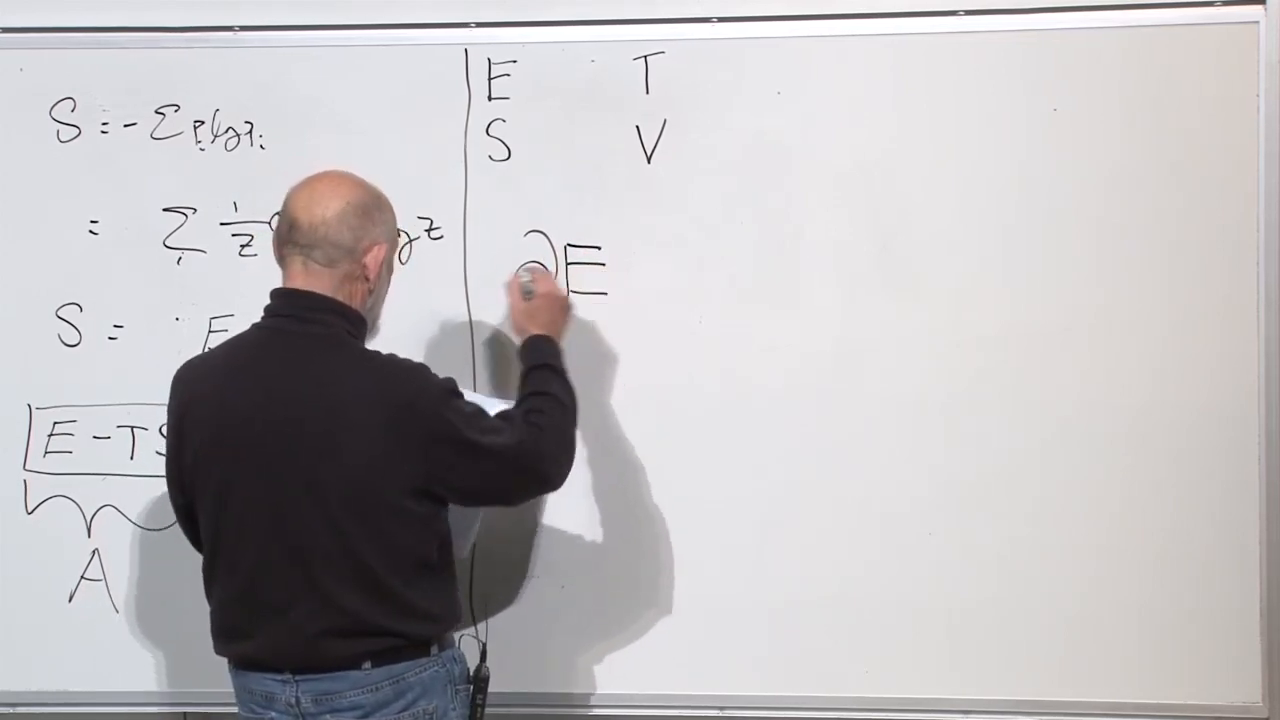
\includegraphics[width=0.90\textwidth]{lecture_05_figure_03.png}\caption{La relation canonique de l’entropie réécrite sous la forme \(A=E-TS=-T\log Z\).}\lectureframe{00:16:50}\end{figure}

\section{Paramètres de contrôle et réponses du système}

Un paramètre de contrôle est une grandeur macroscopique qu’un expérimentateur peut modifier de l’extérieur. Déplacer un piston change le volume sans manipuler les molécules une à une. Les champs électriques et magnétiques appliqués en sont d’autres exemples. Dans un ensemble plus général, le nombre de particules peut lui aussi varier.

Les variables thermodynamiques vont naturellement par paires conjuguées. Dans le problème présent, le volume est le paramètre de contrôle et la pression est la réponse du système. Nous faisons varier \(V\) ; la pression indique la résistance énergétique du système à cette variation. La dérivée de l’énergie précisera plus tard cette association.

\begin{classroomqa}\audiencequestion{Peut-on considérer la pression elle-même comme le paramètre de contrôle ?}\lecturerresponse{On peut concevoir une expérience où la pression extérieure est maintenue fixe, mais dans le montage utilisé ici, la position du piston fixe le volume et la pression intérieure est la réponse du système. La pression et le volume sont des variables conjuguées ; celle que l’on contrôle dépend de l’ensemble et du dispositif expérimental.\lecturetimestamp{00:19:22--00:20:01}}\end{classroomqa}

\begin{classroomqa}\audiencequestion{Suppose-t-on que toutes les molécules sont identiques, ou le raisonnement se limite-t-il à un gaz ?}\lecturerresponse{L’argument thermodynamique n’exige aucune restriction de ce genre. Le cylindre peut contenir plusieurs espèces, un liquide ou même un solide que l’on comprime. La fonction de partition du gaz parfait ne constituera qu’une application particulière, une fois établie la formule générale de la pression.\lecturetimestamp{00:20:02--00:20:39}}\end{classroomqa}

\begin{classroomqa}\audiencequestion{Peut-on aussi modifier la quantité de matière par une autre opération extérieure ?}\lecturerresponse{Oui. Le nombre de particules est un autre paramètre de contrôle possible. Le traiter comme une variable conduit à sa propre variable conjuguée : le potentiel chimique. Pour le calcul de ce soir, \(N\) reste fixe.\lecturetimestamp{00:20:39--00:20:57}}\end{classroomqa}

\begin{classroomqa}\audiencequestion{De l’eau liquide et de la vapeur peuvent-elles coexister à l’équilibre ?}\lecturerresponse{Oui, à la température et à la pression de coexistence. La gravité peut placer le liquide sous la vapeur, mais les deux phases peuvent malgré tout être à la même température et rester en équilibre thermique. Le même cadre général de la mécanique statistique s’applique.\lecturetimestamp{00:20:59--00:21:36}}\end{classroomqa}

Pour le raisonnement qui suit, considérons l’énergie et l’entropie comme des fonctions dépendantes de deux variables que l’on peut régler indépendamment : \begin{equation}
 E=E(T,V),
 \qquad
 S=S(T,V).
 \label{eq:sm5-dependent-functions}
\end{equation} La température et le volume servent de coordonnées dans l’espace des états thermodynamiques. L’énergie et l’entropie attribuent une valeur à chaque point d’équilibre de cet espace.

\section{La dérivée à entropie constante}

La dérivée dont nous aurons finalement besoin est inhabituelle : \[
 \left(\frac{\partial E}{\partial V}\right)_S.
\] Bien que \(T\) et \(V\) soient les coordonnées indépendantes, cette dérivée consiste à faire varier \(V\) tout en imposant à la fonction dépendante \(S(T,V)\) de rester constante. C’est une dérivée le long d’une courbe dans le plan \((T,V)\), et non le long d’un axe de coordonnées.

\begin{classroomqa}\audiencequestion{Comment \(T\) et \(V\) peuvent-ils être indépendants si l’on utilise ensuite la dérivée \(dT/dV\) ?}\lecturerresponse{Ils sont indépendants dans l’ensemble de l’espace des états. Dès que l’on impose la contrainte \(S(T,V)=\mathrm{constant}\), les états accessibles se trouvent sur une courbe unidimensionnelle. Le long de cette courbe, \(T\) devient une fonction de \(V\), et sa pente \(dT/dV\) est bien définie.\lecturetimestamp{01:01:18--01:02:09}}\end{classroomqa}

\begin{lemma}Si \(E(T,V)\) et \(S(T,V)\) sont différentiables, alors, partout où \((\partial S/\partial T)_V\neq0\), \begin{equation}
 \left(\frac{\partial E}{\partial V}\right)_S
 =
 \left(\frac{\partial E}{\partial V}\right)_T
 -
 \left(\frac{\partial E}{\partial S}\right)_V
 \left(\frac{\partial S}{\partial V}\right)_T.
 \label{eq:sm5-calculus-lemma}
\end{equation}\end{lemma}

\begin{proof}Pour un déplacement infinitésimal arbitraire, \begin{equation}
 dE=
 \left(\frac{\partial E}{\partial V}\right)_T dV
 +
 \left(\frac{\partial E}{\partial T}\right)_V dT.
 \label{eq:sm5-total-differential-e}
\end{equation} À \(V\) fixé, la règle de la chaîne permet d’introduire \(S\) comme variable intermédiaire : \begin{equation}
 \left(\frac{\partial E}{\partial T}\right)_V
 =
 \left(\frac{\partial E}{\partial S}\right)_V
 \left(\frac{\partial S}{\partial T}\right)_V.
 \label{eq:sm5-chain-rule-e-s-t}
\end{equation}

Limitons maintenant le déplacement à une courbe sur laquelle \(S\) est constante. Le long de cette courbe, \begin{equation}
 0=dS=
 \left(\frac{\partial S}{\partial V}\right)_T dV
 +
 \left(\frac{\partial S}{\partial T}\right)_V dT.
 \label{eq:sm5-constant-entropy-differential}
\end{equation} En isolant la pente de la courbe, on obtient \begin{equation}
 \left(\frac{dT}{dV}\right)_S
 =
 -
 \frac{\left(\frac{\partial S}{\partial V}\right)_T}
 {\left(\frac{\partial S}{\partial T}\right)_V}.
 \label{eq:sm5-entropy-contour-slope}
\end{equation} Divisons \eqref{eq:sm5-total-differential-e} par \(dV\), utilisons \eqref{eq:sm5-chain-rule-e-s-t} et introduisons \eqref{eq:sm5-entropy-contour-slope} : \begin{align}
 \left(\frac{\partial E}{\partial V}\right)_S
 &=
 \left(\frac{\partial E}{\partial V}\right)_T
 +
 \left(\frac{\partial E}{\partial S}\right)_V
 \left(\frac{\partial S}{\partial T}\right)_V
 \left(\frac{dT}{dV}\right)_S \notag\\
 &=
 \left(\frac{\partial E}{\partial V}\right)_T
 -
 \left(\frac{\partial E}{\partial S}\right)_V
 \left(\frac{\partial S}{\partial V}\right)_T.
\end{align} Le facteur \((\partial S/\partial T)_V\) s’est simplifié, ce qui démontre le résultat.\end{proof}

\begin{figure}[t]\centering
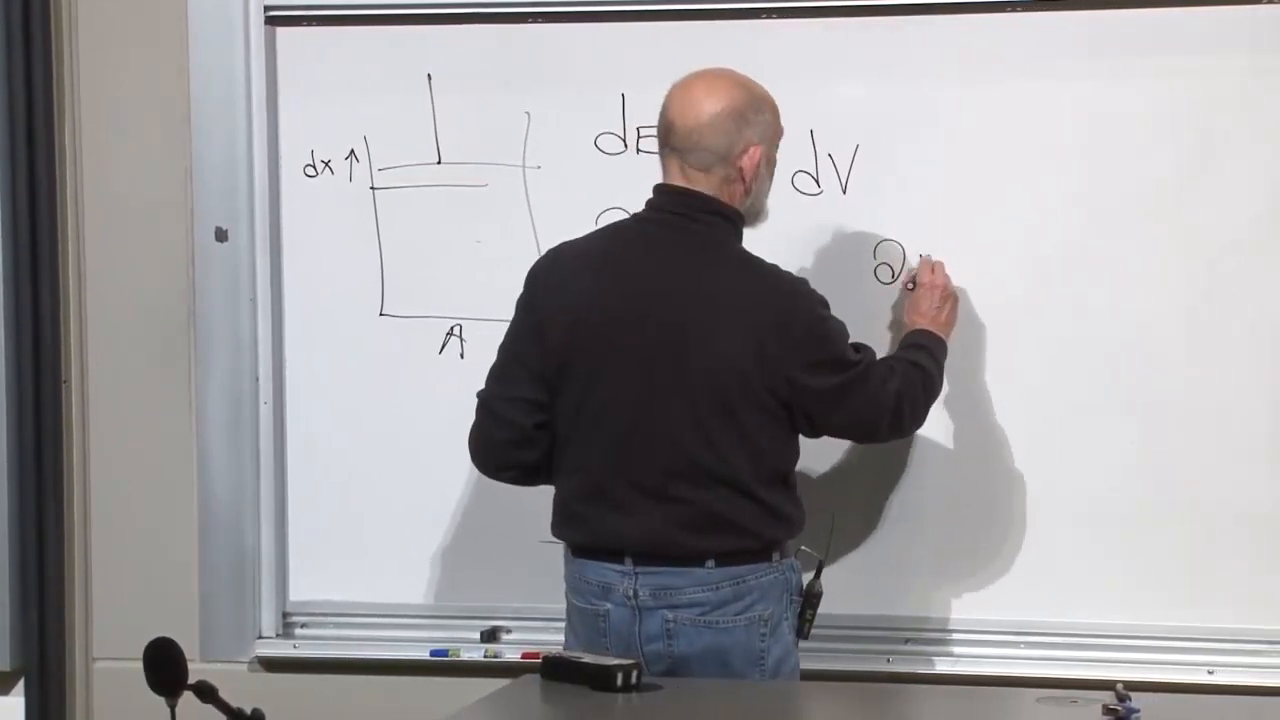
\includegraphics[width=0.90\textwidth]{lecture_05_figure_04.png}\caption{Calcul le long d’une courbe à entropie constante, au stade de la simplification qui achève le lemme sur la dérivée.}\lectureframe{00:36:10}\end{figure}

La représentation géométrique n’est pas décorative. Elle explique pourquoi une dérivée à \(S\) fixé, qui semble étrange, peut se calculer à l’aide des dérivées partielles ordinaires par rapport aux coordonnées indépendantes \(T\) et \(V\). Écrire \(\delta E/\delta V\) pendant la construction rappelle utilement que les symboles représentent des rapports de petites variations le long d’un chemin spécifié.

\begin{classroomqa}\audiencequestion{Le développement de \(dE\) correspond-il simplement à la définition ordinaire des dérivées partielles ?}\lecturerresponse{Oui. Le différentiel total ne présente rien de particulier. Le seul ingrédient supplémentaire est la restriction ultérieure à la courbe \(dS=0\), qui détermine la relation entre \(dT\) et \(dV\).\lecturetimestamp{00:29:26--00:29:32}}\end{classroomqa}

\begin{classroomqa}\audiencequestion{La simplification exige-t-elle que \((\partial S/\partial T)_V\) soit non nul ?}\lecturerresponse{Oui. Pour un système stable ordinaire, \[
 \left(\frac{\partial S}{\partial T}\right)_V
 =\frac{C_V}{T}>0,
\], donc la division est légitime. Les points exceptionnels demandent un examen distinct. À hamiltonien fixé, élever la température élargit la distribution canonique des énergies et augmente normalement l’entropie ; abaisser la température la resserre. C’est le sens physique correct de l’argument de monotonie.\lecturetimestamp{00:36:50--00:37:47}}\end{classroomqa}

\section{Travail du piston et condition adiabatique}

Donnons maintenant une interprétation physique à la dérivée. Considérons un piston de section \(\mathcal A\). S’il se déplace vers l’extérieur d’une distance \(dx\), alors \begin{equation}
 dV=\mathcal A\,dx.
 \label{eq:sm5-piston-volume}
\end{equation} Le gaz exerce sur le piston une force \(P\mathcal A\), donc le travail fourni par le gaz vaut \begin{equation}
 \delta W_{\mathrm{by}}=P\mathcal A\,dx=P\,dV.
 \label{eq:sm5-piston-work}
\end{equation} Si aucune chaleur n’entre dans le gaz, la conservation de l’énergie donne \begin{equation}
 dE=-P\,dV.
 \label{eq:sm5-adiabatic-work}
\end{equation} Le signe a une signification physique : pendant la détente, le gaz soulève ou accélère le piston et son énergie propre diminue.

\begin{figure}[t]\centering
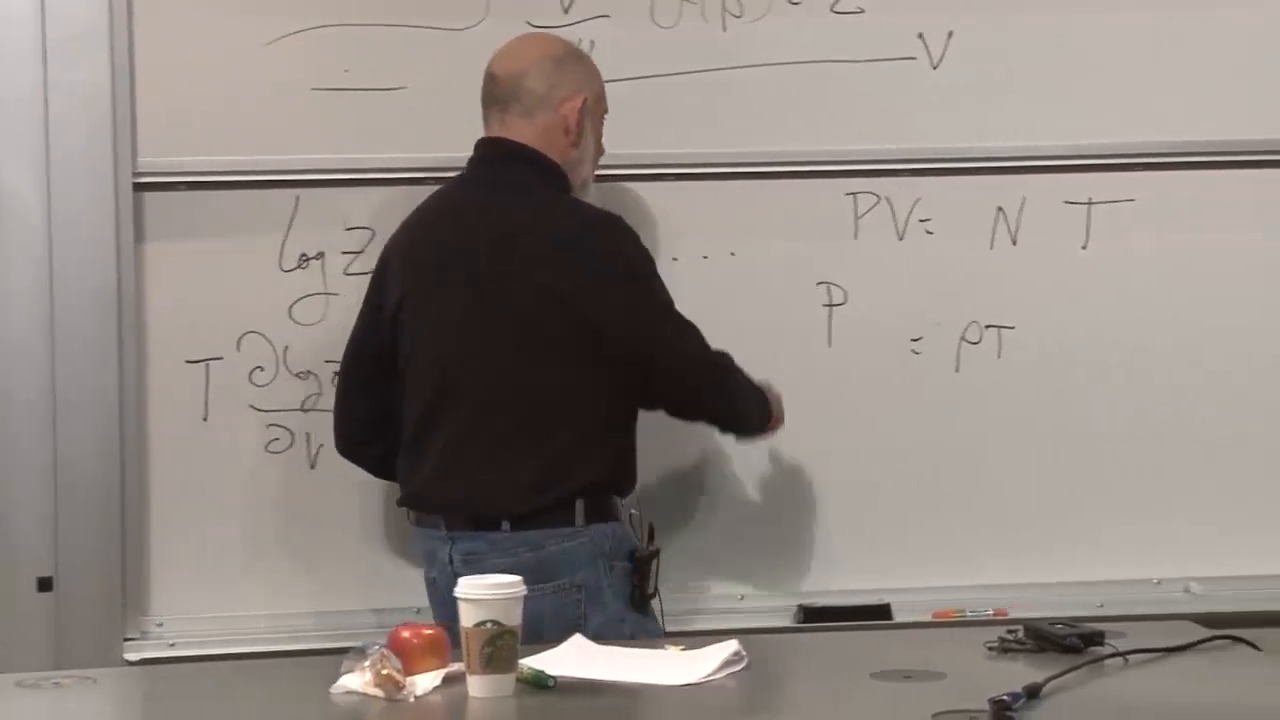
\includegraphics[width=0.90\textwidth]{lecture_05_figure_05.png}\caption{Géométrie du piston et relation de travail obtenue \(dE=-P\,dV\).}\lectureframe{00:43:10}\end{figure}

Deux précisions sont essentielles. Le piston doit se déplacer assez lentement pour que le système reste arbitrairement proche de l’équilibre, et les parois doivent être isolées afin qu’aucune énergie ne soit fournie sous forme de chaleur. Une traction rapide peut être si brusque qu’aucune molécule n’atteigne le piston qui s’éloigne pendant son mouvement. Une compression rapide engendre des ondes de choc. Aucun de ces processus ne peut être décrit comme une succession d’états d’équilibre.

Le terme \emph{adiabatique} désigne parfois l’absence de transfert thermique et parfois une variation lente. Dans le processus réversible requis ici, les deux notions interviennent : la variation est quasi statique et le système est isolé thermiquement. Dans ces conditions, elle est aussi isentropique.

\begin{classroomqa}\audiencequestion{Pourquoi une transformation adiabatique conserve-t-elle l’entropie ?}\lecturerresponse{Considérons le système du point de vue de la mécanique quantique. Ses niveaux d’énergie à plusieurs corps dépendent du volume. Lorsque \(V\) varie lentement, le théorème adiabatique fait évoluer continûment chaque niveau occupé vers le niveau correspondant, sans transition entre les étiquettes des niveaux. Les énergies \(E_i(V)\) varient, mais les probabilités d’occupation \(p_i\) restent fixes. Comme \(S=-\sum_i p_i\log p_i\) dépend de ces probabilités, l’entropie reste constante. Un échange de chaleur ou un mouvement irréversible invaliderait cette conclusion.\lecturetimestamp{00:43:37--00:49:15}}\end{classroomqa}

\begin{figure}[t]\centering
\includegraphics[width=0.90\textwidth]{lecture_05_figure_06.png}\caption{Les niveaux d’énergie à plusieurs corps varient avec le volume tandis que leurs probabilités d’occupation conservent leurs étiquettes de niveau.}\lectureframe{00:48:50}\end{figure}

L’équation \eqref{eq:sm5-adiabatic-work}, évaluée le long de ce chemin à entropie constante, identifie la pression à \begin{equation}
 P=-\left(\frac{\partial E}{\partial V}\right)_S.
 \label{eq:sm5-pressure-fixed-entropy}
\end{equation} C’est la relation de conjugaison entre la pression et le volume.

\begin{classroomqa}\audiencequestion{Que se passe-t-il si le piston se déplace rapidement ?}\lecturerresponse{Le système quitte l’équilibre et sa dynamique détaillée devient pertinente. Une compression brutale engendre une onde de choc. Lors d’une détente libre idéale, le piston peut s’éloigner avant que la moindre molécule ne le heurte : aucun travail n’est alors effectué et l’énergie reste fixe, bien que le volume varie. Le gaz revient ensuite à l’équilibre avec une entropie accrue. Ces processus ne peuvent pas être décrits par l’unique dérivée d’équilibre de \eqref{eq:sm5-pressure-fixed-entropy}.\lecturetimestamp{00:58:30--01:01:15}}\end{classroomqa}

\begin{classroomqa}\audiencequestion{Quelle condition quantitative permet de décider si une variation est lente ?}\lecturerresponse{Le temps caractéristique de la variation extérieure doit être long devant les temps de relaxation internes pertinents. Pour un gaz, de nombreuses collisions moléculaires et de nombreux chocs contre les parois doivent avoir lieu pendant la variation macroscopique. L’échelle de temps précise dépend du matériau et de la géométrie, tandis que la limite quasi statique est générale.\lecturetimestamp{01:02:09--01:03:20}}\end{classroomqa}

\section{De l’énergie adiabatique à la fonction de partition}

La formule physique \eqref{eq:sm5-pressure-fixed-entropy} n’est pas encore la plus facile à calculer. La mécanique statistique canonique fournit naturellement des fonctions de la température, puisque \(T\) apparaît directement dans le facteur de Boltzmann. Le lemme de calcul transforme la dérivée peu commode à entropie fixe en une expression adaptée au calcul : \begin{align}
 P
 &=
 -\left(\frac{\partial E}{\partial V}\right)_T
 +
 \left(\frac{\partial E}{\partial S}\right)_V
 \left(\frac{\partial S}{\partial V}\right)_T.
 \label{eq:sm5-pressure-lemma-substitution}
\end{align} À volume fixe, le premier principe donne \(dE=T\,dS\), et donc \begin{equation}
 \left(\frac{\partial E}{\partial S}\right)_V=T.
 \label{eq:sm5-e-s-temperature}
\end{equation} Ainsi, \begin{equation}
 P=
 -\left(\frac{\partial E}{\partial V}\right)_T
 +
 T\left(\frac{\partial S}{\partial V}\right)_T.
 \label{eq:sm5-pressure-fixed-temperature-pieces}
\end{equation}

\begin{classroomqa}\audiencequestion{D’où vient le signe moins dans la formule de la pression ?}\lecturerresponse{Il provient du travail fourni par le gaz : \(dE=-P\,dV\) lors d’une détente adiabatique. Le lemme de calcul lui-même comporte un signe moins entre ses deux termes ; le signe moins global dans \(P=-(\partial E/\partial V)_S\) inverse les deux, ce qui donne \eqref{eq:sm5-pressure-fixed-temperature-pieces}.\lecturetimestamp{00:52:40--00:53:14}}\end{classroomqa}

Comme \(T\) reste fixe dans les deux dérivées, \begin{align}
 P
 &=
 -\left(\frac{\partial}{\partial V}(E-TS)\right)_T \notag\\
 &=
 -\left(\frac{\partial A}{\partial V}\right)_T.
 \label{eq:sm5-pressure-free-energy}
\end{align} Enfin, introduisons \(A=-T\log Z\) : \begin{equation}
 \boxed{
 P=
 T\left(\frac{\partial\log Z}{\partial V}\right)_T
 }.
 \label{eq:sm5-pressure-log-z}
\end{equation}

\begin{figure}[t]\centering
\includegraphics[width=0.90\textwidth]{lecture_05_figure_07.png}\caption{Le raisonnement à température fixe : \(P=-(\partial A/\partial V)_T
=T(\partial\log Z/\partial V)_T\).}\lectureframe{00:55:55}\end{figure}

Rien dans \eqref{eq:sm5-pressure-log-z} ne suppose que le gaz est parfait. Si l’on peut calculer la fonction de partition d’un fluide avec interactions, d’un plasma ou d’un solide, la même dérivée donne sa pression. Plus généralement, chaque paramètre de contrôle extérieur possède une réponse conjuguée que l’on obtient en dérivant le potentiel thermodynamique approprié. La fonction de partition rassemble bon nombre de ces réponses : sa dérivée \(\log Z\) par rapport à \(\beta\) donne l’énergie, tandis que sa dérivée par rapport au volume donne la pression.

\section{L’équation d’état du gaz parfait}

Spécialisons-nous seulement maintenant au cas de \(N\) particules sans interaction. En conservant la normalisation classique de l’espace des phases, \begin{equation}
 Z_N=
 \frac{1}{N!h^{3N}}
 \int d^{3N}q\,d^{3N}p\,
 \exp\!\left[
 -\beta\sum_{a=1}^{N}\frac{\mathbf p_a^2}{2m}
 \right].
 \label{eq:sm5-ideal-gas-partition-integral}
\end{equation} Il y a \(3N\) coordonnées de position et \(3N\) coordonnées d’impulsion. L’hamiltonien ne dépend pas de la position ; chaque particule apporte donc un facteur égal au volume du récipient : \begin{equation}
 Z_N=
 \frac{V^N}{N!h^{3N}}I_p(\beta),
 \label{eq:sm5-ideal-gas-factorization}
\end{equation} où l’intégrale sur les impulsions entière \(I_p(\beta)\) est indépendante de \(V\).

\begin{classroomqa}\audiencequestion{Pourquoi y a-t-il \(3N\) intégrales sur les positions et \(3N\) intégrales sur les impulsions ?}\lecturerresponse{Chacune des \(N\) particules possède trois coordonnées spatiales et trois composantes d’impulsion conjuguées. Le décompte est de \(3N\) dans chaque moitié de l’espace des phases, et non de \(N\) particules plus \(3N\) autres particules.\lecturetimestamp{01:04:19--01:04:28}}\end{classroomqa}

Un passage au logarithme sépare la dépendance en volume : \begin{equation}
 \log Z_N
 =
 N\log V-\log N!-3N\log h+\log I_p(\beta).
 \label{eq:sm5-log-ideal-gas-partition}
\end{equation} Les facteurs \(1/N!\), \(h^{-3N}\) et \(I_p(\beta)\) sont tous indépendants du volume. Ils importent pour l’entropie absolue et d’autres questions, mais pas pour cette dérivée particulière. Ainsi, \begin{equation}
 \left(\frac{\partial\log Z_N}{\partial V}\right)_T
 =\frac{N}{V}.
 \label{eq:sm5-log-z-volume-derivative}
\end{equation} L’équation \eqref{eq:sm5-pressure-log-z} donne immédiatement \begin{equation}
 P=\frac{NT}{V},
 \qquad
 \boxed{PV=NT}.
 \label{eq:sm5-ideal-gas-law}
\end{equation}

\begin{classroomqa}\audiencequestion{\(N\) compte-t-il encore les répliques utilisées pour déduire la distribution de Boltzmann ?}\lecturerresponse{Non. La construction par répliques était un procédé de dénombrement dans la dérivation précédente ; elle n’intervient plus ici. Dans le présent contexte, \(N\) désigne le nombre de particules physiques dans cet échantillon de gaz.\lecturetimestamp{01:07:38--01:08:05}}\end{classroomqa}

En définissant la densité numérique \begin{equation}
 \rho=\frac{N}{V}
 \label{eq:sm5-number-density}
\end{equation}, on obtient la forme équivalente \begin{equation}
 P=\rho T.
 \label{eq:sm5-density-equation-of-state}
\end{equation}

\begin{classroomqa}\audiencequestion{Faut-il diviser par \(N\) ou par \(V\) pour obtenir l’expression en fonction de la densité ?}\lecturerresponse{Divisez \(PV=NT\) par \(V\) : \(P=(N/V)T=\rho T\). Ici, \(\rho\) désigne la densité numérique, et non la masse volumique.\lecturetimestamp{01:08:45--01:09:16}}\end{classroomqa}

\begin{figure}[t]\centering
\includegraphics[width=0.90\textwidth]{lecture_05_figure_08.png}\caption{La dérivée par rapport au volume de \(\log Z\) et l’équation d’état du gaz parfait qui en résulte, \(PV=NT\), ou \(P=\rho T\).}\lectureframe{01:09:25}\end{figure}

En rétablissant la température de laboratoire \(T_K\), on obtient \begin{equation}
 PV=Nk_BT_K.
 \label{eq:sm5-ideal-gas-law-laboratory}
\end{equation} Le résultat familier concorde avec l’intuition cinétique, mais sa dérivation repose désormais sur un cadre qui s’applique bien au-delà du gaz libre.

\section{Autre résultat : les fluctuations à l’équilibre}

Le calcul de la pression est terminé, mais une question reste en suspens : que peut-on encore tirer de la fonction de partition ? Considérons un système en contact thermique avec un bain. Son énergie n’est pas fixe. L’énergie entre dans le système et en sort ; des mesures répétées fluctuent donc autour de la moyenne canonique.

\begin{classroomqa}\audiencequestion{Pouvons-nous maintenant calculer les fluctuations annoncées ?}\lecturerresponse{Oui. Le temps supplémentaire permet de montrer une nouvelle fois le même principe : les dérivées de \(Z\) encodent des informations thermodynamiques mesurables.\lecturetimestamp{01:10:37--01:10:50}}\end{classroomqa}

\subsection{Variance et écart-type}

Pour une variable aléatoire \(x\) telle que \(\langle x\rangle=0\), une mesure de la largeur de la distribution est \(\langle x^2\rangle\). Pour une distribution quelconque, décalons la variable de sa moyenne : \begin{equation}
 \delta x=x-\langle x\rangle.
 \label{eq:sm5-centered-variable}
\end{equation} Sa moyenne est nulle, \begin{equation}
 \langle\delta x\rangle
 =
 \langle x\rangle-\langle x\rangle=0,
 \label{eq:sm5-centered-mean}
\end{equation} et sa moyenne quadratique vaut \begin{align}
 (\Delta x)^2
 &\equiv
 \left\langle\left(x-\langle x\rangle\right)^2\right\rangle \notag\\
 &=
 \langle x^2\rangle
 -2\langle x\rangle^2
 +\langle x\rangle^2 \notag\\
 &=
 \langle x^2\rangle-\langle x\rangle^2.
 \label{eq:sm5-variance}
\end{align} C’est la variance. Sa racine carrée positive \(\Delta x\) est l’écart-type.

\begin{classroomqa}\audiencequestion{Pourquoi la moyenne de \(x-\langle x\rangle\) est-elle exactement nulle ?}\lecturerresponse{La moyenne est une opération linéaire, et \(\langle x\rangle\) est déjà un nombre. On a donc \(\langle x-\langle x\rangle\rangle
=\langle x\rangle-\langle x\rangle=0\).\lecturetimestamp{01:14:02--01:14:22}}\end{classroomqa}

\begin{classroomqa}\audiencequestion{Quelle différence y a-t-il entre le carré de la fluctuation, la variance, la largeur quadratique moyenne et l’écart-type ?}\lecturerresponse{La variance vaut \((\Delta x)^2=\langle x^2\rangle-\langle x\rangle^2\). L’écart-type est sa racine carrée, \(\Delta x\). Pour une variable de moyenne nulle, l’écart-type est aussi sa valeur quadratique moyenne.\lecturetimestamp{01:16:39--01:18:38}}\end{classroomqa}

\begin{figure}[t]\centering
\includegraphics[width=0.90\textwidth]{lecture_05_figure_09.png}\caption{La variable décentrée et le développement qui donne \((\Delta x)^2=\langle x^2\rangle-\langle x\rangle^2\).}\lectureframe{01:17:20}\end{figure}

\subsection{Moments de l’énergie tirés de la fonction de partition}

Dans l’ensemble canonique, \begin{align}
 \langle E\rangle
 &=
 \frac{1}{Z}\sum_i E_i e^{-\beta E_i} \notag\\
 &=
 -\frac{1}{Z}\frac{\partial Z}{\partial\beta}
 =
 -\frac{\partial\log Z}{\partial\beta}.
 \label{eq:sm5-mean-energy-from-z}
\end{align} Multiplier par un facteur \(E_i\) revient à prendre une dérivée par rapport à \(\beta\), avec un signe moins. Une seconde dérivée produit \(E_i^2\) : \begin{equation}
 \langle E^2\rangle
 =
 \frac{1}{Z}\sum_i E_i^2e^{-\beta E_i}
 =
 \frac{1}{Z}\frac{\partial^2 Z}{\partial\beta^2}.
 \label{eq:sm5-second-energy-moment}
\end{equation} La variance de l’énergie vaut donc \begin{align}
 (\Delta E)^2
 &=
 \langle E^2\rangle-\langle E\rangle^2 \notag\\
 &=
 \frac{1}{Z}\frac{\partial^2Z}{\partial\beta^2}
 -
 \frac{1}{Z^2}
 \left(\frac{\partial Z}{\partial\beta}\right)^2 \notag\\
 &=
 \frac{\partial^2\log Z}{\partial\beta^2}
 =
 -\frac{\partial\langle E\rangle}{\partial\beta}.
 \label{eq:sm5-energy-variance-beta}
\end{align} Une fois encore, une observable d’apparence complexe se ramène à une dérivée de \(\log Z\).

\begin{figure}[t]\centering
\includegraphics[width=0.90\textwidth]{lecture_05_figure_10.png}\caption{La dérivée seconde par rapport à \(\beta\) de \(\log Z\), identifiée à la variance de l’énergie.}\lectureframe{01:29:00}\end{figure}

\subsection{Capacité thermique et amplitude des fluctuations}

Dans les unités du cours \(T=1/\beta\), donc \begin{equation}
 -\frac{\partial}{\partial\beta}
 =
 T^2\frac{\partial}{\partial T}.
 \label{eq:sm5-beta-temperature-derivative}
\end{equation} Définissons, à volume fixe, la capacité thermique de l’échantillon entier par \begin{equation}
 C_V\equiv
 \left(\frac{\partial\langle E\rangle}{\partial T}\right)_V.
 \label{eq:sm5-heat-capacity}
\end{equation} L’équation \eqref{eq:sm5-energy-variance-beta} devient \begin{equation}
 \boxed{(\Delta E)^2=T^2C_V}
 \qquad (k_B=1).
 \label{eq:sm5-energy-fluctuation-lecture-units}
\end{equation} Pour la température de laboratoire \(T_K\), où \(\beta=(k_BT_K)^{-1}\), \begin{equation}
 \boxed{(\Delta E)^2=k_BT_K^2C_V}.
 \label{eq:sm5-energy-fluctuation-laboratory}
\end{equation}

\begin{figure}[t]\centering
\includegraphics[width=0.90\textwidth]{lecture_05_figure_11.png}\caption{Passage de la dérivée par rapport à \(\beta\) à la capacité thermique à volume fixe, avec rétablissement du facteur \(k_B\).}\lectureframe{01:31:10}\end{figure}

\begin{classroomqa}\audiencequestion{Faut-il préciser que la dérivée est prise à volume fixe plutôt qu’à pression fixe ?}\lecturerresponse{Oui. Cette dérivation canonique maintient fixes les paramètres de contrôle extérieurs de l’hamiltonien, y compris \(V\). La grandeur obtenue est \(C_V\). Dans un ensemble à pression constante, le volume et le travail peuvent fluctuer, et il faut utiliser le potentiel thermodynamique correspondant ; on ne peut pas simplement remplacer \(C_V\) par \(C_P\) dans \eqref{eq:sm5-energy-fluctuation-laboratory}.\lecturetimestamp{01:29:01--01:29:28; 01:32:50--01:33:21}}\end{classroomqa}

\begin{classroomqa}\audiencequestion{\(C_V\)est-ce une constante du matériau ?}\lecturerresponse{Pas en général. Elle peut dépendre de la température, du volume, de la phase et de la composition. De plus, \(C_V\) désigne ici la capacité thermique de l’échantillon entier ; c’est une grandeur extensive. On n’obtient une chaleur massique qu’en divisant par la masse, le nombre de particules ou la quantité de matière.\lecturetimestamp{01:31:47--01:32:21; 01:33:23--01:34:55}}\end{classroomqa}

Pour une matière ordinaire extensive, \(C_V\) est proportionnelle à \(N\), donc \((\Delta E)^2\) est proportionnelle à \(N\) et \(\Delta E\) à \(\sqrt{N}\). L’énergie moyenne elle-même est proportionnelle à \(N\). Par conséquent, \begin{equation}
 \frac{\Delta E}{\langle E\rangle}\sim\frac{1}{\sqrt{N}}.
 \label{eq:sm5-relative-fluctuation-scaling}
\end{equation} Les fluctuations relatives sont infimes à l’échelle macroscopique, tandis que les échantillons microscopiques les révèlent directement. La présence de \(k_B\) dans \eqref{eq:sm5-energy-fluctuation-laboratory} marque ce lien entre les observables thermodynamiques et le caractère discret des molécules ; de manière équivalente, elle relie les unités macroscopiques au dénombrement à l’échelle du nombre d’Avogadro.

La pression et les fluctuations découlent désormais d’un même objet : \[
 P=T\left(\frac{\partial\log Z}{\partial V}\right)_T,
 \qquad
 (\Delta E)^2=\frac{\partial^2\log Z}{\partial\beta^2}.
\] C’est la leçon essentielle. Une fois les bonnes contraintes identifiées, la fonction de partition ne sert pas seulement à normaliser les probabilités. Ses dérivées organisent les grandeurs thermodynamiques mesurables du système.
\chapter{Interactions faibles, corrections du viriel et différentielles inexactes}

\lectureoverview{Nous commençons par le sens opérationnel de la mesure et de la température, puis nous examinons comment un gaz dilué s’écarte de la loi des gaz parfaits lorsqu’on introduit progressivement de faibles interactions à courte portée. La fonction de partition fournit les premières corrections dues aux interactions pour l’énergie et la pression, et en précise le domaine de validité. Un dernier détour mathématique distingue les fonctions d’état de la chaleur et du travail, qui dépendent du chemin suivi, au moyen des différentielles exactes, des boucles fermées et d’un exemple concret de gaz parfait.}

\section{Ce que mesure réellement un instrument}

Aucun appareil de laboratoire ne puise directement dans la nature pour rendre compte d’une variable mathématique abstraite. Un dynamomètre indique un allongement ; un thermomètre, la hauteur d’une colonne de liquide. Nous parlons de mesure d’une force dans le premier cas et de mesure d’une température dans le second uniquement parce qu’une relation reproductible a été établie entre la réponse observable et la grandeur recherchée.

Cette relation n’est valable que dans un domaine limité. Un ressort n’obéit à la loi de Hooke que tant qu’il reste élastique ; si la force devient suffisamment grande, il finit par se déformer ou se rompre. Plus généralement, si une indication lisse \(R\) dépend d’une variable physique \(X\), alors au voisinage d’un point de fonctionnement choisi,
\begin{equation}
 \Delta R \simeq
 \left.\frac{dR}{dX}\right|_{X_0}\Delta X.
 \label{eq:sm6-local-linear-response}
\end{equation}
les petites variations de l’indication sont proportionnelles aux petites variations de la variable recherchée, même lorsque la réponse complète est non linéaire. Cette linéarisation locale relève de la méthode ordinaire d’étalonnage.

L’indication peut aussi dépendre de variables parasites. Un ressort peut réagir faiblement à la température ou à la pression. La hauteur du mercure dans un thermomètre pourrait dépendre de l’orientation sous l’effet de la gravité, des propriétés du verre ou de l’évolution lente des matériaux. Un protocole de mesure ne prouve pas l’absence de ces dépendances : il les maintient constantes ou montre qu’elles sont négligeables à l’échelle requise.

\begin{classroomqa}
\audiencequestion{Le champ gravitationnel local, ou l’orientation du thermomètre, peut-il modifier la lecture ?}
\lecturerresponse{Oui, en principe. Si l’orientation a un effet appréciable, l’instruction de tenir le thermomètre à la verticale fait partie de la définition de l’instrument. À la surface de la Terre, le champ gravitationnel est suffisamment stable pour que les variations résiduelles soient normalement négligeables.
\lecturetimestamp{00:04:08--00:05:00}}
\end{classroomqa}

\begin{classroomqa}
\audiencequestion{Le vieillissement ou une évolution chimique peuvent-ils modifier lentement l’étalonnage ?}
\lecturerresponse{C’est possible. Le mercure et le verre sont suffisamment inertes pour les mesures courantes, tandis que les changements sur des échelles de temps extraordinairement longues n’ont pas d’importance pour l’expérience. Tout étalonnage se rapporte à un instrument, un domaine, un protocole et une durée spécifiés.
\lecturetimestamp{00:05:03--00:06:11}}
\end{classroomqa}

Pour un thermomètre Celsius, deux états de référence reproductibles fournissent une échelle commode. Si \(h_f\) et \(h_b\) désignent respectivement les hauteurs de la colonne aux points de congélation et d’ébullition de l’eau, alors, dans un domaine où la réponse est presque linéaire,
\begin{equation}
 T_{\mathrm C}=100\,\frac{h-h_f}{h_b-h_f}.
 \label{eq:sm6-celsius-calibration}
\end{equation}
Le choix de \(T_{\mathrm C}=0\) au point de congélation est conventionnel. Il ne correspond pas à l’état d’énergie thermique nulle, pas plus que zéro degré Fahrenheit par une journée d’hiver ne correspond au zéro absolu.

\begin{figure}[t]
\centering
\includegraphics[width=0.90\textwidth]{lecture_06_figure_03.png}
\caption{Réponse lisse mais non linéaire d’un thermomètre, avec un court intervalle délimité pour l’étalonnage linéaire.}
\lectureframe{00:07:55}
\end{figure}

\section{Équilibre et température comme échelle d’énergie}

Un thermomètre ne mesure la température de son environnement qu’une fois que lui-même et le milieu voisin ont atteint l’équilibre thermique. Avant cela, sa lecture ne fait qu’évoluer vers l’équilibre. Le critère pratique est simple : attendre que la lecture cesse de changer. Cette règle apparemment simple dissimule les processus physiques qui déterminent le temps d’attente.

\begin{classroomqa}
\audiencequestion{L’équilibration ne concerne-t-elle qu’une couche limite autour du bulbe, et combien de temps faut-il attendre ?}
\lecturerresponse{L’énergie doit traverser le verre et être échangée avec le milieu environnant ; le temps dépend donc du thermomètre, de sa conductivité thermique et du milieu. L’environnement immédiat doit aussi être représentatif d’un état d’équilibre uniforme. En pratique, on considère que la mesure est acquise lorsqu’elle ne dérive plus.
\lecturetimestamp{00:08:45--00:10:13}}
\end{classroomqa}

La température et la densité jouent des rôles distincts dans ce temps d’attente. Un gaz très dilué peut être très chaud : les quelques molécules présentes peuvent avoir de grandes énergies cinétiques. Pourtant, elles heurtent rarement le thermomètre, si bien que l’équilibration peut être lente. Réduire la densité d’un facteur cent ou mille tout en maintenant la température constante ne diminue pas l’échelle d’énergie moléculaire ; cela réduit la vitesse à laquelle cette énergie est transmise à l’instrument.

\begin{classroomqa}
\audiencequestion{Le rayonnement dans une pièce peut-il avoir une température différente de celle de l’air ?}
\lecturerresponse{Oui. Matière et rayonnement n’ont une température commune que lorsqu’ils sont en équilibre thermique l’un avec l’autre. L’air neutre interagit faiblement avec une grande partie du rayonnement optique dans une pièce éclairée ; la population de photons n’est donc pas nécessairement un champ de rayonnement de corps noir à l’équilibre à la température de l’air.
\lecturetimestamp{00:11:26--00:12:20}}
\end{classroomqa}

Une fois l’équilibre établi, il est préférable de considérer la température comme une échelle d’énergie. Nous continuons à utiliser les unités où \(k_B=1\), de sorte que \(T\) a elle-même les dimensions d’une énergie. Pour un gaz parfait monoatomique,
\begin{equation}
 E_0=\frac{3}{2}NT.
 \label{eq:sm6-ideal-energy}
\end{equation}
L’énergie thermique par molécule est fixée par \(T\) ; la vitesse correspondante dépend toujours de la masse moléculaire.

\section{Introduire une faible interaction}

\begin{classroomqa}
\audiencequestion{Dans quelles conditions l’approximation du gaz parfait cesse-t-elle d’être valable, et peut-on montrer mathématiquement cet écart ?}
\lecturerresponse{Partons du gaz non interactif, dont la solution est connue, et introduisons une faible interaction. Développons en fonction de cette perturbation, calculons la première correction et comparons-la au terme idéal. L’approximation cesse d’être valable lorsque la correction n’est plus petite.
\lecturetimestamp{00:12:25--00:14:40}}
\end{classroomqa}

C’est la stratégie perturbative classique. Si un problème est soluble pour \(\lambda=0\), introduisons un couplage \(\lambda\), écrivons
\begin{equation}
 F(\lambda)=F(0)+\lambda F_1+\lambda^2F_2+\cdots,
 \label{eq:sm6-perturbative-template}
\end{equation}
et vérifions si chaque terme retenu est plus petit que le précédent. Ici, le problème de référence est celui du gaz parfait. Le faible paramètre physique tient à la dilution de l’échantillon, à une portée de l’interaction courte devant la distance moyenne entre molécules, et à un potentiel assez faible pour que le premier terme d’interaction soit pertinent. Une forte densité ou une force de longue portée peut invalider l’approximation, même si chaque rencontre prise isolément semble peu intense.

Soient \(x_i\in\mathbb R^3\) et \(p_i\in\mathbb R^3\) la position et la quantité de mouvement de la molécule \(i\). Pour des molécules identiques de masse \(m\), prenons
\begin{equation}
 H(X,P)=
 \sum_{i=1}^{N}\frac{p_i^2}{2m}
 +\sum_{i<j}u\!\left(|x_i-x_j|\right),
 \label{eq:sm6-interacting-hamiltonian}
\end{equation}
où \(X=(x_1,\ldots,x_N)\) et \(P=(p_1,\ldots,p_N)\). La restriction \(i<j\) exclut les paires d’une particule avec elle-même et ne compte chaque paire \((i,j)\) qu’une seule fois :
\begin{equation}
 \sum_{i<j}1=\binom{N}{2}=\frac{N(N-1)}{2}.
 \label{eq:sm6-pair-count}
\end{equation}

\begin{classroomqa}
\audiencequestion{Pourquoi ne pas sommer séparément sur les deux indices des particules ?}
\lecturerresponse{La paire \((3,7)\) est la même paire physique que \((7,3)\), et une particule n’est pas appariée avec elle-même. Restreindre la somme à \(i<j\) impose ces deux conditions. On réserve le symbole de masse \(m\), tandis que \(i,j\) désignent les particules, afin d’éviter la collision de notation qui se produirait si \(m\) désignait les deux.
\lecturetimestamp{00:17:52--00:19:12}}
\end{classroomqa}

Écrivons le potentiel configurationnel total sous la forme
\begin{equation}
 U(X)=\sum_{i<j}u\!\left(|x_i-x_j|\right).
 \label{eq:sm6-total-potential}
\end{equation}
On suppose l’interaction invariante par translation et de courte portée : \(u(r)\) devient négligeable lorsque \(r\) est grand devant une longueur moléculaire.

\section{L’intensité intégrée de la paire}

Une seule intégrale du faible potentiel de paire intervient dans la première correction :
\begin{equation}
 U_0\equiv\int_{\mathbb R^3}d^3r\,u(r).
 \label{eq:sm6-u0-definition}
\end{equation}
Ses unités sont celles d’une énergie multipliée par un volume. Elle combine l’intensité typique de l’interaction et le volume sur lequel celle-ci est appréciable.

\begin{figure}[t]
\centering
\includegraphics[width=0.90\textwidth]{lecture_06_figure_04.png}
\caption{Le potentiel de paire à courte portée ramené à l’intensité intégrée \(U_0=\int d^3r\,u(r)\).}
\lectureframe{00:25:15}
\end{figure}

Pour voir pourquoi \(U_0\) est utile, considérons une paire :
\begin{equation}
 I_2=\int_V d^3x_1\,d^3x_2\,
 u\!\left(|x_1-x_2|\right).
 \label{eq:sm6-two-particle-integral}
\end{equation}
Introduisons une coordonnée relative \(r=x_2-x_1\). Loin de la frontière, l’intégrale relative donne \(U_0\), tandis que la position commune de la paire parcourt tout le récipient. Ainsi,
\begin{equation}
 I_2=V U_0+\text{surface corrections}.
 \label{eq:sm6-pair-integral-vu0}
\end{equation}
La correction vient des particules situées à une portée d’interaction du bord, où une partie du voisinage en coordonnée relative se trouve hors de la boîte. Son importance relative est proportionnelle au rapport surface-volume et s’annule dans la limite macroscopique.

\begin{classroomqa}
\audiencequestion{\(U_0\) désigne-t-il une paire donnée, et l’une des particules reste-t-elle à une distance fixe de l’autre ?}
\lecturerresponse{Il désigne la loi d’interaction commune à toute paire. Fixons la première particule et intégrons sur toutes les positions relatives de la seconde. La séparation n’est pas fixe au cours de cette intégration. Seule la région où l’interaction est proche contribue de façon appréciable, ce qui donne \(U_0\).
\lecturetimestamp{00:26:03--00:27:33}}
\end{classroomqa}

\begin{classroomqa}
\audiencequestion{Pourquoi l’intégrale sur la position de la seconde particule donne-t-elle le volume complet du récipient, alors que celle sur la première ne le donne pas ?}
\lecturerresponse{Une fois la configuration relative intégrée dans \(U_0\), la paire entière peut être translatée dans l’échantillon. Cette translation commune fournit le grand facteur \(V\). Le voisinage d’interaction est un volume de l’échelle moléculaire, déjà contenu dans \(U_0\), et non un facteur supplémentaire égal au volume du récipient.
\lecturetimestamp{00:27:48--00:29:21}}
\end{classroomqa}

\begin{classroomqa}
\audiencequestion{La valeur peut-elle dépendre du point fixé, surtout près d’une paroi ?}
\lecturerresponse{L’invariance par translation rend la valeur dans le volume indépendante du point fixé. Près d’une paroi, l’intégrale diffère légèrement parce que certaines positions voisines sont inaccessibles. Seule une couche superficielle d’épaisseur moléculaire est concernée ; l’erreur est donc négligeable lorsque la boîte est macroscopique.
\lecturetimestamp{00:29:24--00:31:22}}
\end{classroomqa}

\begin{classroomqa}
\audiencequestion{Le résultat est-il l’énergie potentielle intégrée sur toutes les configurations à deux particules, et pourquoi est-il proportionnel à un seul grand volume ?}
\lecturerresponse{Oui. Ses unités sont celles d’une énergie multipliée par un volume au carré, puisque \(V U_0\) contient un volume de récipient et un volume d’interaction moléculaire. Seul le premier croît avec la taille de l’échantillon.
\lecturetimestamp{00:31:31--00:32:04}}
\end{classroomqa}

\begin{classroomqa}
\audiencequestion{Choisir une sphère, qui minimise la surface à volume fixé, change-t-il le résultat dans le volume ?}
\lecturerresponse{Cela ne modifie que la petite correction de bord. Pour toute forme macroscopique ordinaire, le nombre de particules situées à une distance moléculaire de la surface est négligeable devant le nombre de particules dans le volume. La surface ne devient importante que lorsque le récipient lui-même approche l’échelle moléculaire.
\lecturetimestamp{00:32:04--00:33:58}}
\end{classroomqa}

\begin{classroomqa}
\audiencequestion{A-t-on omis les collisions en remplaçant les trajectoires des particules par un potentiel ?}
\lecturerresponse{Non. La force est la dérivée du potentiel et c’est précisément elle qui produit les collisions. La mécanique statistique à l’équilibre n’exige pas de suivre ces collisions une à une : leur effet est encodé dans l’énergie et donc dans le facteur de Boltzmann.
\lecturetimestamp{00:33:59--00:35:29}}
\end{classroomqa}

\begin{classroomqa}
\audiencequestion{Que perd-on en ne gardant que les forces de paire et en omettant les véritables interactions à trois corps ?}
\lecturerresponse{Une énergie microscopique peut comporter de véritables termes à trois corps, et les ordres supérieurs d’un potentiel de paire produisent aussi des corrélations entre plusieurs particules. Dans un gaz dilué, toutefois, la probabilité que trois particules données occupent un même voisinage moléculaire est bien plus faible que celle que deux particules le fassent. Les effets de paire fournissent donc la première correction en densité ; les amas d’ordre supérieur interviennent aux puissances supérieures de la densité.
\lecturetimestamp{00:35:29--00:38:14}}
\end{classroomqa}

\section{La fonction de partition, sans détour}

L’avantage de la méthode statistique apparaît maintenant. Une fois l’hamiltonien spécifié, nul besoin de deviner la distribution détaillée des vitesses près des parois ou pendant les collisions. Écrivons la fonction de partition canonique et suivons les étapes du calcul :
\begin{equation}
\begin{aligned}
 Z&=
 \frac{1}{N!h^{3N}}
 \int d^{3N}P\,d^{3N}X\\
 &\qquad{}\times e^{-\beta K(P)}e^{-\beta U(X)},\\
 K(P)&=\sum_i\frac{p_i^2}{2m}.
\end{aligned}
 \label{eq:sm6-full-partition-function}
\end{equation}
Le facteur \(h^{3N}\) rend sans dimension la mesure classique dans l’espace des phases, et \(N!\) élimine le surcomptage dû aux permutations de particules identiques.

\begin{figure}[t]
\centering
\includegraphics[width=0.90\textwidth]{lecture_06_figure_05.png}
\caption{Énergie d’un système de nombreuses particules et facteurs cinétique et configurationnel correspondants dans la fonction de partition.}
\lectureframe{00:40:35}
\end{figure}

La quantité de mouvement et la position se séparent. En multipliant et en divisant l’intégrale configurationnelle par \(V^N\), isolons le résultat du gaz parfait :
\begin{align}
 Z
 &=\left[
 \frac{V^N}{N!h^{3N}}
 \int d^{3N}P\,e^{-\beta K(P)}
 \right] \notag\\
 &\quad\times\left[
 \frac{1}{V^N}
 \int d^{3N}X\,e^{-\beta U(X)}
 \right] \notag\\
 &\equiv Z_0\,C(\beta,V,N).
 \label{eq:sm6-z-factorization}
\end{align}
Le facteur gaussien bien connu vaut
\begin{equation}
 \int d^{3N}P\,e^{-\beta K(P)}
 =\left(\frac{2\pi m}{\beta}\right)^{3N/2}.
 \label{eq:sm6-gaussian-factor}
\end{equation}

\begin{figure}[t]
\centering
\includegraphics[width=0.90\textwidth]{lecture_06_figure_06.png}
\caption{Fonction de partition du gaz parfait isolée du facteur configurationnel normalisé.}
\lectureframe{00:43:45}
\end{figure}

Le facteur \(N!\) n’affecte ni le rapport normalisé \(C\), ni les dérivées à \(N\) fixé utilisées ci-dessous. Il n’est toutefois pas dispensable en thermodynamique dans son ensemble : il est essentiel au dénombrement correct des états et à l’extensivité de l’entropie.

Au premier ordre en l’interaction,
\begin{equation}
 e^{-\beta U(X)}
 =1-\beta U(X)+O(U^2).
 \label{eq:sm6-boltzmann-expansion}
\end{equation}
Par conséquent,
\begin{align}
 C
 &=
 1-\frac{\beta}{V^N}
 \sum_{i<j}
 \int d^{3N}X\,u(|x_i-x_j|)
 +O(U^2) \notag\\
 &=
 1-\frac{\beta}{V^N}
 \frac{N(N-1)}{2}
 V^{N-2}(V U_0)+O(U^2) \notag\\
 &=
 1-\beta\frac{N(N-1)}{2V}U_0+O(U^2).
 \label{eq:sm6-configurational-correction}
\end{align}
Chaque paire a la même \emph{intégrale}, et non la même séparation instantanée ni la même énergie potentielle. Les \(N-2\) intégrales restantes sur les positions apportent chacune un facteur \(V\).

\begin{figure}[t]
\centering
\includegraphics[width=0.90\textwidth]{lecture_06_figure_07.png}
\caption{Comptage des paires, volumes associés aux coordonnées spectatrices et première correction configurationnelle \(1-\beta N^2U_0/(2V)\).}
\lectureframe{00:53:40}
\end{figure}

\begin{classroomqa}
\audiencequestion{Le terme dominant \(1\) suppose-t-il que le potentiel s’annule à séparation nulle ?}
\lecturerresponse{Non. C’est le terme d’ordre zéro du développement de l’exponentielle, indépendant de la valeur de \(u(0)\). Le potentiel intervient au terme suivant, \(-\beta U(X)\).
\lecturetimestamp{00:46:19--00:46:48}}
\end{classroomqa}

\begin{classroomqa}
\audiencequestion{Pourquoi peut-on remplacer chaque paire par la même expression si leurs séparations diffèrent ?}
\lecturerresponse{On n’assimile pas leurs valeurs ponctuelles. Chaque terme est intégré sur le même espace complet des configurations, et les étiquettes des particules ne distinguent pas une paire d’une autre. Les intégrales ont la même forme et la même valeur.
\lecturetimestamp{00:50:00--00:51:07}}
\end{classroomqa}

\begin{classroomqa}
\audiencequestion{Le nombre de paires est-il \(N(N-1)/2\) ou \(N(N+1)/2\) ?}
\lecturerresponse{C’est \(N(N-1)/2\) : après avoir choisi une particule, il ne reste que \(N-1\) partenaires distincts, et la division par deux élimine le double comptage des deux ordres. Pour un \(N\) macroscopique, remplacer \(N(N-1)\) par \(N^2\) ne modifie le résultat que d’une correction relative de l’ordre de \(1/N\).
\lecturetimestamp{00:48:33--00:49:56}}
\end{classroomqa}

Comme \(\log(1-x)=-x-x^2/2-x^3/3-\cdots\), et non une série alternée, le logarithme au premier ordre est
\begin{equation}
 \log Z
 =
 \log Z_0
 -\beta\frac{N(N-1)}{2V}U_0
 +O(U^2).
 \label{eq:sm6-logz-correction}
\end{equation}
Pour un grand \(N\), nous pouvons remplacer \(N(N-1)\) par \(N^2\), puisque aucune distinction à nombre fini de \(N\) n’est nécessaire.

\begin{remark}La formulation contrôlée à faible densité utilise la fonction de Mayer \(f(r)=e^{-\beta u(r)}-1\) et le deuxième coefficient du viriel
\begin{equation}
 B_2(T)=-\frac{1}{2}\int d^3r\,f(r).
 \label{eq:sm6-second-virial}
\end{equation}
Pour un potentiel faible, \(f(r)\simeq-\beta u(r)\), donc \(B_2\simeq\beta U_0/2\), et l’on retrouve le résultat ci-dessous. Cette formulation est nécessaire pour un cœur répulsif dur, pour lequel le développement direct de \(e^{-\beta u}\) n’est pas valable.
\end{remark}

\section{Énergie, pression et sens de la correction}

Le logarithme de \(Z\) est utile parce que ses dérivées sont mesurables. En supposant que le potentiel microscopique est indépendant de la température,
\begin{align}
 E
 &=-\left(\frac{\partial\log Z}{\partial\beta}\right)_{V,N} \notag\\
 &=
 \frac{3}{2}NT
 +\frac{N(N-1)}{2V}U_0+O(U^2) \notag\\
 &\simeq
 N\left(\frac{3}{2}T+\frac{1}{2}\rho U_0\right),
 \qquad
 \rho=\frac{N}{V}.
 \label{eq:sm6-energy-correction}
\end{align}
Le terme en apparence non extensif \(N^2\) s’accompagne de \(1/V\). À densité fixée, \(N^2/V=N\rho\), de sorte que l’énergie totale reste proportionnelle à la taille du système. L’énergie supplémentaire par particule est proportionnelle à la densité, car une molécule donnée n’acquiert une énergie de paire que lorsqu’une autre molécule se trouve à proximité.

\begin{figure}[t]
\centering
\includegraphics[width=0.90\textwidth]{lecture_06_figure_08.png}
\caption{La première correction due aux interactions, réécrite sous la forme d’une énergie extensive \(N[3T/2+\rho U_0/2]\).}
\lectureframe{01:03:25}
\end{figure}

La pression est plus facile à mesurer. En utilisant le résultat du chapitre précédent,
\begin{equation}
 P=T\left(\frac{\partial\log Z}{\partial V}\right)_{T,N},
 \label{eq:sm6-pressure-from-z}
\end{equation}
on obtient
\begin{align}
 P
 &=
 \frac{NT}{V}
 +T\frac{\partial}{\partial V}
 \left(-\beta\frac{N(N-1)}{2V}U_0\right)
 +O(U^2) \notag\\
 &=
 \rho T+\frac{1}{2}\rho^2U_0
 +O\!\left(\frac{\rho U_0}{N},U^2\right).
 \label{eq:sm6-pressure-correction}
\end{align}

\begin{figure}[t]
\centering
\includegraphics[width=0.90\textwidth]{lecture_06_figure_09.png}
\caption{Pression obtenue à partir de la dérivée de Helmholtz, avec la première correction quadratique en densité.}
\lectureframe{01:09:50}
\end{figure}

\begin{classroomqa}
\audiencequestion{Pourquoi \(\rho^2\) constitue-t-il la correction initiale naturelle, plutôt qu’une autre puissance ?}
\lecturerresponse{Le terme idéal exige la présence d’une particule dans une petite région et est donc proportionnel à \(\rho\). Une interaction exige que deux particules occupent un même voisinage moléculaire, ce dont la probabilité est proportionnelle à \(\rho^2\). Le facteur \(1/2\) est le même facteur de comptage des paires qui empêche de compter séparément \((i,j)\) et \((j,i)\).
\lecturetimestamp{01:24:27--01:26:00}}
\end{classroomqa}

À température fixée, on peut faire varier \(V\), mesurer \(\rho=N/V\) et tracer la pression. La loi idéale donne le terme linéaire. La courbure de \(P(\rho)\) révèle la première correction due aux interactions. Dans le cadre de cette approximation de potentiel faible, la correction ne dépend pas explicitement de la température, car le facteur \(T\) dans \eqref{eq:sm6-pressure-from-z} s’annule avec \(\beta=1/T\).

\begin{classroomqa}
\audiencequestion{Jusqu’à quelle densité peut-on aller avant de devoir prendre en compte les effets à trois corps ?}
\lecturerresponse{Le dénombrement en densité indique que le terme suivant du viriel est proportionnel à \(\rho^3\), mais son coefficient ne peut pas être déduit de \(U_0\) seul. Il reçoit des contributions de produits corrélés d’interactions de paire et, le cas échéant, de véritables forces à trois corps. Il faut calculer le coefficient d’amas suivant et le comparer au terme en \(\rho^2\) ; une formule conjecturée ne doit pas être présentée comme un résultat.
\lecturetimestamp{01:10:50--01:13:38}}
\end{classroomqa}

Le terme du gaz parfait domine lorsque la correction est faible en valeur absolue :
\begin{equation}
 \begin{aligned}
 \frac{1}{2}\rho^2|U_0|&\ll \rho T,\\
 |\rho U_0|&\ll T
 \qquad\text{(parametrically)}.
 \end{aligned}
 \label{eq:sm6-ideal-validity}
\end{equation}
Les deux membres de la seconde inégalité sont des énergies. La grandeur \(\rho U_0\) est l’échelle de l’énergie d’interaction par particule, tandis que \(T\) est l’échelle de l’énergie cinétique. Un gaz dilué ordinaire à température ambiante se trouve largement dans ce régime ; des écarts notables apparaissent seulement lorsque les voisinages moléculaires sont assez souvent occupés pour que les interactions rivalisent avec l’agitation thermique.

\begin{classroomqa}
\audiencequestion{Peut-on estimer ce critère pour l’air de cette pièce ?}
\lecturerresponse{Estimons \(U_0\) comme le produit d’une énergie d’interaction moléculaire par un volume moléculaire, multiplions-le par la densité numérique et comparons le résultat à \(k_BT\). Les ordres de grandeur moléculaires montrent que l’échelle d’interaction est bien plus faible dans l’air ambiant ordinaire. Il faut une compression considérable avant que les molécules se retrouvent souvent à portée d’interaction les unes des autres.
\lecturetimestamp{01:16:24--01:18:54}}
\end{classroomqa}

\begin{classroomqa}
\audiencequestion{\(U_0\) peut-il être de l’un ou l’autre signe ?}
\lecturerresponse{Oui. Une interaction intégrée positive est globalement répulsive dans cette approximation et élève la pression au-dessus de \(\rho T\). Une valeur négative correspond à une attraction nette et l’abaisse. Ce test de signe fournit une vérification physique immédiate de \eqref{eq:sm6-pressure-correction}.
\lecturetimestamp{01:18:56--01:20:29}}
\end{classroomqa}

\begin{figure}[t]
\centering
\includegraphics[width=0.90\textwidth]{lecture_06_figure_10.png}
\caption{Profils qualitatifs de potentiels de paire répulsif et attractif, à côté de la formule de pression dont la correction suit le signe de \(U_0\).}
\lectureframe{01:21:30}
\end{figure}

\begin{classroomqa}
\audiencequestion{Peut-on introduire dans ce calcul la répulsion électrostatique, l’attraction gravitationnelle ou les forces moléculaires réelles ?}
\lecturerresponse{Le potentiel microscopique provient de la physique atomique, moléculaire ou quantique. Les molécules neutres présentent souvent un cœur répulsif à courte portée très raide et une queue attractive de van der Waals de plus grande portée, représentés schématiquement par un potentiel 12--6. Pour un tel cœur dur, il faut utiliser la formule complète faisant intervenir la fonction de Mayer. La gravité est différente : sa portée est longue, son intégrale spatiale ne converge pas de la manière requise, et la limite thermodynamique ordinaire à courte portée utilisée ici ne s’applique pas.
\lecturetimestamp{01:20:40--01:23:03}}
\end{classroomqa}

Ce calcul illustre une répartition utile des rôles. La physique microscopique fournit \(u(r)\). La mécanique statistique transforme cette énergie en \(Z\) ; les dérivées de \(Z\) donnent les observables macroscopiques, et le raisonnement physique en vérifie le signe, la dépendance en densité, l’extensivité et le domaine de validité. Le calcul formel ne devient mécanique qu’une fois choisies l’énergie correcte et l’approximation appropriée.

\section{Différentielles exactes et dépendance du chemin}

Nous adoptons maintenant un autre langage mathématique. Dans l’expression \emph{différentielle exacte}, « exacte » ne signifie pas numériquement précise. Cela signifie qu’une forme différentielle est la différentielle d’une véritable fonction scalaire.

Soit \(f(x,y)\) l’altitude au-dessus d’un point du paysage. Un petit déplacement la fait varier de
\begin{equation}
 df=
 \frac{\partial f}{\partial x}\,dx+
 \frac{\partial f}{\partial y}\,dy
 =f_x\,dx+f_y\,dy.
 \label{eq:sm6-total-differential}
\end{equation}
Supposons plutôt qu’on nous donne simplement
\begin{equation}
 \omega=F_x(x,y)\,dx+F_y(x,y)\,dy.
 \label{eq:sm6-one-form}
\end{equation}
Existe-t-il un scalaire \(f\) tel que \(\omega=df\) ? L’égalité des dérivées partielles mixtes impose
\begin{equation}
 \frac{\partial F_y}{\partial x}
 =
 \frac{\partial F_x}{\partial y}.
 \label{eq:sm6-exactness-condition}
\end{equation}
Sur un domaine simplement connexe, cette condition de rotationnel nul est également suffisante. Les composantes \((F_x,F_y)\) forment alors le gradient de \(f\).

\begin{figure}[t]
\centering
\includegraphics[width=0.90\textwidth]{lecture_06_figure_11.png}
\caption{Altitude comme fonction scalaire, sa différentielle et condition sur les dérivées partielles mixtes garantissant l’exactitude.}
\lectureframe{01:34:30}
\end{figure}

La même condition a une interprétation intégrale. Si \(\omega=df\), alors
\begin{equation}
 \int_{\gamma:1\to2}\omega=f(2)-f(1)
 \label{eq:sm6-path-independent-integral}
\end{equation}
ne dépend que des extrémités, et non du chemin \(\gamma\). En particulier,
\begin{equation}
 \oint_\gamma\omega=0
 \label{eq:sm6-closed-loop-zero}
\end{equation}
pour toute boucle fermée contractile.

L’altitude possède cette propriété. Aller d’un même point à un autre par une route de niveau ou en franchissant une colline donne la même variation nette d’altitude. Ce n’est pas le cas de la consommation de carburant. Un itinéraire vallonné et un itinéraire plat consomment généralement des quantités différentes, et un trajet en boucle ne restitue pas le carburant brûlé. La quantité de carburant restant est certes bien définie si l’on élargit la description de l’état, mais elle n’est pas une fonction de la seule position \((x,y)\) de la voiture : elle garde la mémoire du trajet. La fatigue fournit une analogie du même type : descendre une colline n’annule généralement pas la fatigue accumulée en la gravissant.

\begin{classroomqa}
\audiencequestion{L’exactitude est-elle la même notion que celle d’une force conservative, et a-t-elle un lien avec la courbure ?}
\lecturerresponse{Un champ de forces de rotationnel nul est localement conservatif et admet un potentiel ; les deux notions sont donc étroitement liées. Le transport parallèle et la courbure relient aussi les variations le long de boucles fermées à des propriétés géométriques locales, mais cela relève d’un sujet plus vaste. Ici, seule l’affirmation élémentaire est nécessaire : un rotationnel nul entraîne l’indépendance locale du chemin, sous réserve de la condition globale habituelle sur le domaine.
\lecturetimestamp{01:39:22--01:41:07}}
\end{classroomqa}

Deux exemples rendent le critère concret. Prenons d’abord
\begin{equation}
 F_x=y,\qquad F_y=x.
 \label{eq:sm6-exact-example}
\end{equation}
Les deux dérivées croisées valent \(1\), et l’on a bien
\begin{equation}
 \omega=y\,dx+x\,dy=d(xy).
 \label{eq:sm6-exact-example-potential}
\end{equation}
Changeons maintenant un signe :
\begin{equation}
 F_x=y,\qquad F_y=-x.
 \label{eq:sm6-inexact-example}
\end{equation}
Alors,
\begin{equation}
 \frac{\partial F_x}{\partial y}=1,
 \qquad
 \frac{\partial F_y}{\partial x}=-1,
 \label{eq:sm6-inexact-cross-derivatives}
\end{equation}
si bien qu’aucun scalaire \(f(x,y)\) n’a ces deux composantes pour gradient.

\begin{figure}[t]
\centering
\includegraphics[width=0.90\textwidth]{lecture_06_figure_12.png}
\caption{Exemple exact engendré par \(f=xy\) et exemple inexact dont les dérivées croisées valent \(1\) et \(-1\).}
\lectureframe{01:44:50}
\end{figure}

\section{La chaleur et le travail ne sont pas des fonctions d’état}

Pour un système compressible simple à nombre de particules fixé, deux variables d’équilibre indépendantes déterminent l’état. On peut choisir \((T,V)\), \((E,V)\) ou, ce qui est particulièrement naturel pour la relation fondamentale, \((S,V)\). Ainsi,
\begin{equation}
 E=E(S,V),
 \end{equation}
et sa différentielle exacte est
\begin{equation}
 dE=
 \left(\frac{\partial E}{\partial S}\right)_V dS+
 \left(\frac{\partial E}{\partial V}\right)_S dV
 =T\,dS-P\,dV.
 \label{eq:sm6-fundamental-relation}
\end{equation}

\begin{classroomqa}
\audiencequestion{Adiabatique signifie-t-il lent, isolé, réversible ou à entropie constante ?}
\lecturerresponse{La terminologie varie selon les contextes. Pour le chemin d’équilibre considéré ici, la transformation est quasi statique et thermiquement isolée ; elle est donc réversible et isentropique. Un processus simplement isolé peut néanmoins être irréversible et produire de l’entropie, tandis que le théorème quantique de l’adiabaticité met l’accent sur une variation lente des paramètres.
\lecturetimestamp{01:47:13--01:47:54}}
\end{classroomqa}

À entropie constante, une détente fait varier l’énergie du gaz de \(-P\,dV\). À volume constant, un transfert réversible de chaleur la fait varier de \(T\,dS\). Il est donc utile d’écrire
\begin{equation}
 \begin{aligned}
 \delta W_{\mathrm{on}}&=-P\,dV,
 &\delta Q_{\mathrm{rev}}&=T\,dS,\\
 dE&=\delta Q_{\mathrm{rev}}+\delta W_{\mathrm{on}}.&&
 \end{aligned}
 \label{eq:sm6-first-law-increments}
\end{equation}
Le symbole \(\delta\), plutôt que \(d\), indique que la chaleur et le travail sont des incréments dépendant du chemin, et non les différentielles de fonctions d’état.

\begin{figure}[t]
\centering
\includegraphics[width=0.90\textwidth]{lecture_06_figure_13.png}
\caption{Premier principe pour un système à piston :
\(dE=-P\,dV+T\,dS\).}
\lectureframe{01:50:28}
\end{figure}

\begin{classroomqa}
\audiencequestion{L’expression \(-P\,dV\) représente-t-elle le travail effectué sur le gaz ou par le gaz ?}
\lecturerresponse{Avec la convention de \eqref{eq:sm6-first-law-increments}, il s’agit du travail effectué sur le gaz. Lors d’une expansion \(dV>0\), le gaz effectue un travail positif sur le piston ; le travail effectué sur le gaz est donc négatif et le gaz perd de l’énergie. Les deux descriptions sont égales et de signe opposé.
\lecturetimestamp{01:51:23--01:52:27}}
\end{classroomqa}

L’égalité \(\delta Q_{\mathrm{rev}}=T\,dS\) ne doit pas être étendue telle quelle au chauffage irréversible arbitraire. En général,
\begin{equation}
 dS=\frac{\delta Q}{T_{\mathrm{boundary}}}+dS_{\mathrm{prod}},
 \qquad dS_{\mathrm{prod}}\ge 0.
 \label{eq:sm6-entropy-production}
\end{equation}
L’argument sur les différentielles exactes présenté ci-dessous concerne les chemins d’équilibre quasi statiques, pour lesquels la relation réversible est appropriée.

\begin{classroomqa}
\audiencequestion{Suppose-t-on que tous les chemins de l’argument dans l’espace des états passent par des états d’équilibre ?}
\lecturerresponse{Oui. Les opérations sont effectuées assez lentement pour que \(P\), \(T\), \(E\), \(S\) et \(V\) restent bien définis le long du chemin. La dépendance de la chaleur et du travail vis-à-vis du chemin n’exige pas que le système soit éloigné de l’équilibre.
\lecturetimestamp{01:54:30--01:54:39}}
\end{classroomqa}

Pour tester si la chaleur est une différentielle exacte, prenons \((E,V)\) comme coordonnées et réarrangeons le premier principe :
\begin{equation}
 \delta Q_{\mathrm{rev}}=dE+P(E,V)\,dV.
 \label{eq:sm6-heat-one-form}
\end{equation}
S’il existait une fonction d’état \(Q(E,V)\) telle que \(dQ=\delta Q_{\mathrm{rev}}\), ses dérivées partielles devraient être
\begin{equation}
 \left(\frac{\partial Q}{\partial E}\right)_V=1,
 \qquad
 \left(\frac{\partial Q}{\partial V}\right)_E=P.
 \label{eq:sm6-hypothetical-heat-derivatives}
\end{equation}
L’égalité des dérivées mixtes imposerait alors
\begin{equation}
 \begin{aligned}
 \frac{\partial}{\partial V}
 \left(\frac{\partial Q}{\partial E}\right)_V
 &=\frac{\partial}{\partial E}
 \left(\frac{\partial Q}{\partial V}\right)_E,\\
 0&=\left(\frac{\partial P}{\partial E}\right)_V.
 \end{aligned}
 \label{eq:sm6-heat-exactness-requirement}
\end{equation}

\begin{classroomqa}
\audiencequestion{Est-ce exactement le même test du rotationnel que pour \(F_x\,dx+F_y\,dy\) ?}
\lecturerresponse{Oui. Les coefficients de \(dE\) et \(dV\) sont \(1\) et \(P(E,V)\). Leurs dérivées croisées sont \(0\) et \((\partial P/\partial E)_V\). La chaleur ne serait une différentielle exacte que si ces dérivées étaient égales.
\lecturetimestamp{01:54:39--01:54:52}}
\end{classroomqa}

\begin{figure}[t]
\centering
\includegraphics[width=0.90\textwidth]{lecture_06_figure_14.png}
\caption{La forme différentielle de la chaleur \(dE+P\,dV\) et les dérivées mixtes qu’exigerait le fait qu’elle soit la différentielle d’une fonction d’état.}
\lectureframe{01:58:10}
\end{figure}

Cette condition est déjà physiquement peu plausible : ajouter de l’énergie à un gaz à volume constant modifie généralement sa pression. Le gaz parfait fournit un calcul direct :
\begin{equation}
 PV=NT,
 \qquad
 E=\frac{3}{2}NT
 \quad\Longrightarrow\quad
 P=\frac{2E}{3V}.
 \label{eq:sm6-ideal-pressure-energy}
\end{equation}
On obtient donc
\begin{equation}
 \left(\frac{\partial P}{\partial E}\right)_V
 =\frac{2}{3V}\ne0.
 \label{eq:sm6-heat-curl-fails}
\end{equation}
Le test du rotationnel échoue : \(\delta Q_{\mathrm{rev}}\) n’est pas une différentielle exacte. L’incrément de travail \(\delta W_{\mathrm{on}}=-P\,dV\) échoue pour la même raison.

\begin{figure}[t]
\centering
\includegraphics[width=0.90\textwidth]{lecture_06_figure_15.png}
\caption{Les relations du gaz parfait réunies donnent \(P=2E/(3V)\).}
\lectureframe{02:00:00}
\end{figure}

\begin{figure}[H]
\centering
\includegraphics[width=0.90\textwidth]{lecture_06_figure_16.png}
\caption{L’argument complet : puisque \((\partial P/\partial E)_V\ne0\), la forme différentielle de la chaleur ne peut pas être exacte.}
\lectureframe{02:00:35}
\end{figure}

Pour un cycle d’équilibre fermé,
\begin{equation}
 \oint dE=0,
 \qquad
 \oint\delta Q_{\mathrm{rev}}
 =-\oint\delta W_{\mathrm{on}}.
 \label{eq:sm6-cycle-balance}
\end{equation}
Le système retrouve la même énergie, mais la chaleur et le travail ne sont pas nécessairement nuls séparément. Leurs valeurs dépendent du chemin parcouru dans l’espace des états. C’est pourquoi un moteur cyclique peut absorber de la chaleur et fournir un travail net alors que son fluide de travail revient à son état thermodynamique initial.

\begin{classroomqa}
\audiencequestion{Cette dépendance au chemin est-elle liée au rendement des moteurs, à l’hystérésis et à la mémoire ?}
\lecturerresponse{Les cycles des moteurs l’exploitent directement : sur un cycle fermé, la chaleur reçue compense le travail net fourni tandis que la fonction d’état \(E\) retrouve sa valeur initiale. L’hystérésis et la mémoire font également intervenir une dépendance au chemin, même si elles nécessitent souvent des variables internes supplémentaires ou une physique hors équilibre. La conclusion présente est plus restreinte et vaut déjà pour les chemins d’équilibre réversibles : la chaleur et le travail sont des transferts, pas des propriétés stockées dans l’état thermodynamique.
\lecturetimestamp{02:02:21--02:03:17}}
\end{classroomqa}

Les deux volets de l’argument se rejoignent maintenant. Une mesure n’a de sens qu’une fois précisés ses paramètres de contrôle et ses conditions d’équilibre. Une approximation n’a de sens qu’une fois précisés son petit paramètre et son critère d’échec. Une grandeur thermodynamique est une fonction d’état uniquement si sa différentielle satisfait au critère d’indépendance du chemin. Dans chaque cas, les mathématiques rigoureuses ne remplacent pas l’interprétation physique ; elles indiquent précisément dans quelles conditions cette interprétation est justifiée.
\chapter{Son, oscillateurs quantiques et deuxième principe}

\lectureoverview{Le deuxième principe est le point d’arrivée, mais deux calculs concrets nous y préparent. La vitesse du son montre comment des dérivées thermodynamiques deviennent un mouvement observable. L’oscillateur harmonique met ensuite en évidence l’échec de l’équipartition classique pour les degrés de liberté rigides et montre comment la mécanique quantique active les modes un à un. Enfin, nous reviendrons au conflit apparent entre la dynamique microscopique réversible et l’augmentation de l’entropie. Nous nous appuierons sur l’écoulement dans l’espace des phases, le coarse-graining, le chaos et la récurrence pour énoncer le deuxième principe comme une loi extrêmement probable, plutôt que comme une interdiction mécanique sans exception.}

\section{Une promesse au sujet du deuxième principe}

Le problème central est facile à énoncer, mais difficile à expliquer. Les équations newtoniennes sont réversibles : si une évolution microscopique est possible, son évolution renversée dans le temps l’est aussi. Pourtant, le deuxième principe affirme que les processus macroscopiques ont un sens privilégié, caractérisé par une entropie qui, en règle générale, augmente. Nous aborderons cette tension, mais pas tout de suite. Mieux vaut d’abord voir la mécanique statistique fournir des résultats concrets, puis rencontrer, dans le cadre d’un calcul élémentaire, le problème historique qui a contraint la physique classique à céder la place à la physique quantique.

Le premier exemple est numérique et volontairement approximatif : estimons la vitesse du son dans un gaz dilué. Le deuxième est exact dans le cadre de ses hypothèses : calculons l’énergie moyenne d’un oscillateur harmonique dans un bain thermique. L’oscillateur nous conduira de l’équipartition aux niveaux d’énergie quantifiés, d’un mode à une infinité de modes, puis à la question de savoir ce que signifie, pour un système à plusieurs particules, oublier son état initial.

\section{L’échelle moléculaire de la vitesse du son}

Imaginons une légère surdensité dans un gaz dilué. Elle se résorbe parce que des molécules quittent la région où elles sont concentrées ; sa vitesse de propagation devrait donc être comparable à la vitesse moléculaire. L’équipartition donne l’énergie cinétique d’une molécule, \begin{equation}
 \frac{3}{2}k_B T
 =\frac{1}{2}m\expect{v^2},
 \qquad
 \expect{v^2}=\frac{3k_B T}{m}.
 \label{eq:sm7-molecular-speed}
\end{equation}Ici, la température est mesurée à partir du zéro absolu, et \(k_B\) a été rétablie parce que nous voulons utiliser les unités de laboratoire. Il ne s’agit que d’une estimation d’ordre de grandeur : la vitesse quadratique moyenne des molécules n’est pas en soi la vitesse d’une onde sonore collective.

Une dérivation plus systématique considère un petit élément de gaz. Des pressions différentes sur ses faces opposées exercent une force résultante, et son accélération est inversement proportionnelle à la masse volumique. On obtient une expression de la forme \begin{equation}
 c_s^2=
 \left(\frac{\partial P}{\partial \rho_m}\right)_{\cal C},
 \qquad
 \rho_m=m\rho,
 \label{eq:sm7-sound-general}
\end{equation}où \(\rho\) désigne la densité numérique et l’indice \({\cal C}\) précise la condition thermodynamique suivie par la perturbation. Le calcul au tableau utilise \begin{equation}
 P=\rho k_B T
 \quad\Longrightarrow\quad
 \frac{1}{m}
 \left(\frac{\partial P}{\partial\rho}\right)_T
 =\frac{k_B T}{m}.
 \label{eq:sm7-sound-isothermal}
\end{equation}Il s’agit de l’estimation isotherme de la vitesse du son. Elle diffère de \eqref{eq:sm7-molecular-speed} d’un facteur \(3\) pour le carré de la vitesse, ou de \(\sqrt{3}\) pour la vitesse elle-même.

\begin{figure}[t]
\centering
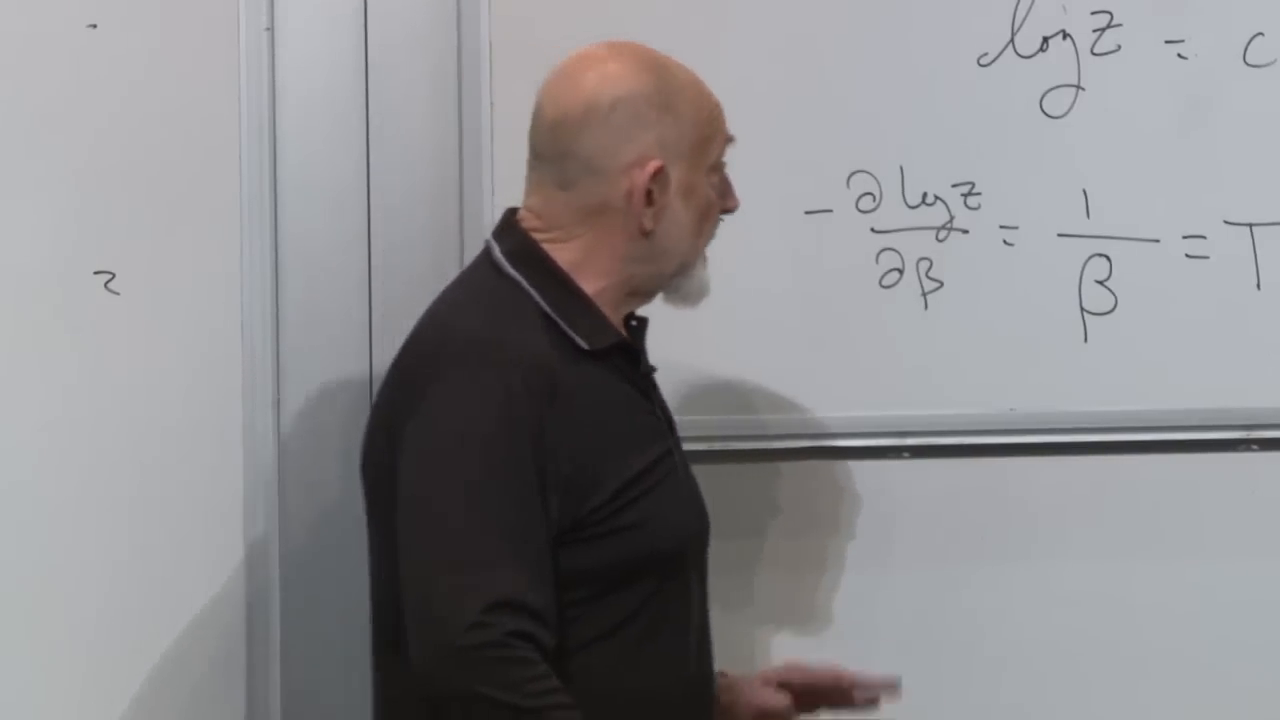
\includegraphics[width=0.90\textwidth]{lecture_07_figure_02.png}
\caption{Estimation de la vitesse moléculaire, dérivée de la pression et substitution du gaz parfait, présentées ensemble.}
\lectureframe{00:08:55}
\end{figure}

Il y a une correction importante à apporter. Une onde sonore de faible amplitude comprime et détend généralement le gaz plus vite que la chaleur ne peut circuler entre les éléments voisins. Le mouvement local est donc approximativement adiabatique, et non isotherme : \begin{equation}
 c_s^2=
 \left(\frac{\partial P}{\partial\rho_m}\right)_S.
 \label{eq:sm7-sound-adiabatic}
\end{equation}Pour un gaz parfait d’indice adiabatique \(\gamma\), \begin{equation}
 P\rho_m^{-\gamma}=\text{constant},
 \qquad
 c_s^2=\gamma\frac{P}{\rho_m}
       =\gamma\frac{k_B T}{m}.
 \label{eq:sm7-sound-ideal-adiabatic}
\end{equation}Pour l’air diatomique à température ambiante, \(\gamma\simeq 7/5\). Le calcul à température fixe constitue donc une première estimation utile, tandis que la dérivée adiabatique apporte la correction physiquement appropriée.

En prenant les valeurs approximatives \begin{equation}
\begin{aligned}
 k_B&\simeq1.3\times10^{-23}\ {\rm J\,K^{-1}},
 &T&\simeq300\ {\rm K},\\
 m_{\rm air}&\simeq4\times10^{-26}\ {\rm kg}.&&
\end{aligned}
 \label{eq:sm7-air-data}
\end{equation}l’estimation moléculaire vaut environ \(500\ {\rm m\,s^{-1}}\). La température doit ici être une température absolue, exprimée en kelvins, et non une échelle décalée comme celle de Fahrenheit. La vitesse du son familière est de l’ordre de \(300\ {\rm m\,s^{-1}}\), et la formule adiabatique du gaz parfait donne environ \(340\ {\rm m\,s^{-1}}\) à température ambiante. Le calcul approximatif a donc permis de trouver le bon ordre de grandeur physique.

\begin{figure}[t]
\centering
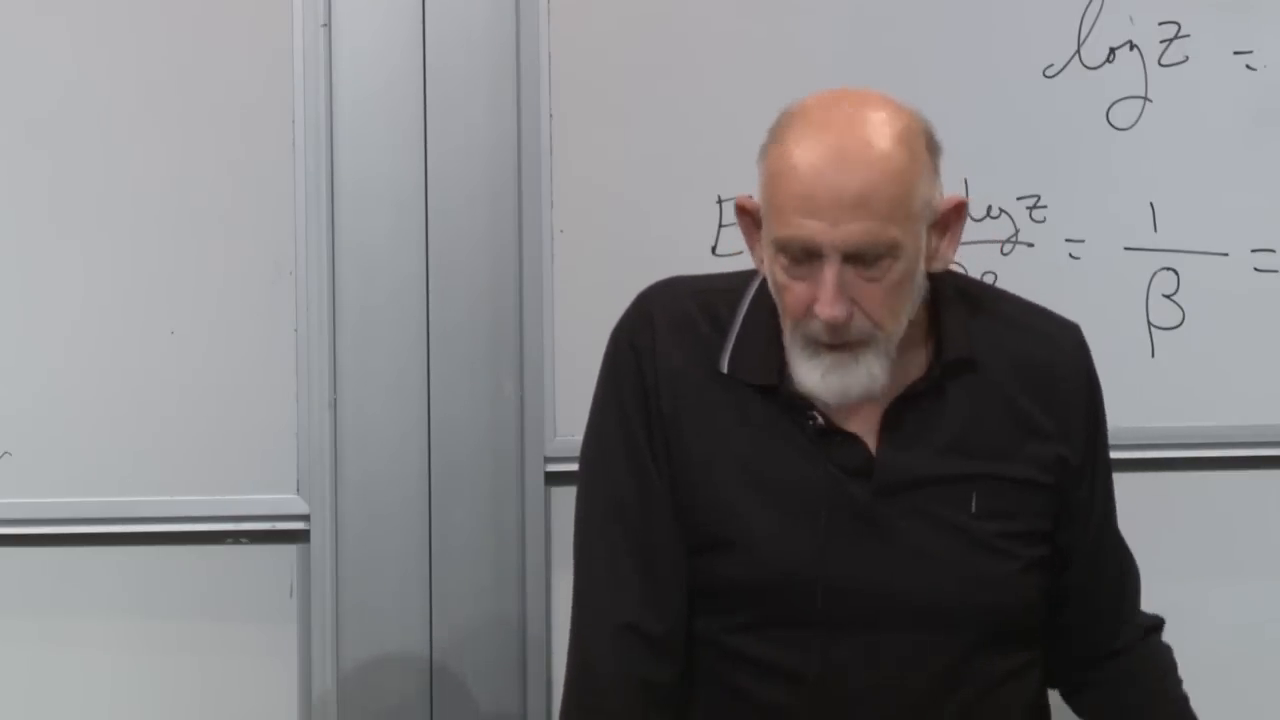
\includegraphics[width=0.90\textwidth]{lecture_07_figure_03.png}
\caption{Estimation pour l’air ambiant à l’aide de la constante de Boltzmann, d’une masse moléculaire effective proche de \(30\) masses du proton et de \(T\simeq300\ {\rm K}\).}
\lectureframe{00:10:55}
\end{figure}

Bien avant qu’une description microscopique soit disponible, on pouvait déterminer la vitesse du son en mesurant la pression en fonction de la densité. Le raisonnement statistique ajoute cette interprétation frappante : la vitesse macroscopique obtenue est fixée par la vitesse thermique des molécules individuelles.

\begin{classroomqa}
\audiencequestion{Faut-il ajouter les neutrons à la masse moléculaire, et le nombre \(14\) pour l’azote compte-t-il seulement les protons ?}
\lecturerresponse{La masse atomique citée compte déjà les protons et les neutrons. Une molécule d’azote contient deux atomes de masse atomique voisine de \(14\) ; sa masse vaut donc environ \(28\) masses du proton. Pour cette estimation, il suffit d’arrondir \(28\) à \(30\).
\lecturetimestamp{00:10:58--00:11:16}}
\end{classroomqa}

\begin{classroomqa}
\audiencequestion{Le facteur \(3\) vient des trois directions de translation, alors que le son se propage dans une seule direction. Faut-il donc supprimer le facteur \(3\) ?}
\lecturerresponse{Cette question nous rappelle à juste titre qu’il ne faut pas confondre la vitesse quadratique moyenne tridimensionnelle des molécules avec une vitesse de propagation unidimensionnelle. L’argument initial ne donnait qu’un ordre de grandeur. Pour obtenir une réponse contrôlée, il faut utiliser la dérivée de la pression et la condition thermodynamique appropriée à l’onde.
\lecturetimestamp{00:11:12--00:12:00}}
\end{classroomqa}

\begin{classroomqa}
\audiencequestion{La dérivée supposait-elle que la température reste constante pendant l’onde ?}
\lecturerresponse{C’était le cas de la substitution affichée pour le gaz parfait. Maintenir la température constante constitue une estimation provisoire plausible pour une perturbation très faible ; la correction usuelle consiste à considérer que le son ordinaire est approximativement adiabatique, ce qui remplace la dérivée isotherme par \(\left(\partial P/\partial\rho_m\right)_S\).
\lecturetimestamp{00:12:59--00:14:01}}
\end{classroomqa}

\begin{classroomqa}
\audiencequestion{Si les variations de pression et de densité sont toutes deux faibles, leur dérivée est-elle alors faible ?}
\lecturerresponse{Non. Une dérivée est le rapport de deux faibles variations dans la limite infinitésimale. \(\delta P\) et \(\delta\rho\) peuvent toutes deux être faibles, tandis que \(\delta P/\delta\rho\) reste finie et fixe la vitesse de l’onde.
\lecturetimestamp{00:14:03--00:14:23}}
\end{classroomqa}

\begin{classroomqa}
\audiencequestion{La vitesse du son devrait-elle augmenter lorsque le gaz est comprimé, comme c’est le cas lorsqu’on passe d’un gaz à un liquide ou à un solide ?}
\lecturerresponse{Oui. La dérivée est évaluée dans l’état considéré, et \(P(\rho,T)\) n’est pas nécessairement une fonction linéaire. Lorsque les molécules sont comprimées et rapprochées, l’équation d’état devient non idéale et \(\partial P/\partial\rho\) peut augmenter considérablement.
\lecturetimestamp{00:14:25--00:15:13}}
\end{classroomqa}

\begin{classroomqa}
\audiencequestion{La valeur \(500\ {\rm m\,s^{-1}}\) est-elle valable à toutes les pressions ?}
\lecturerresponse{Non. Elle correspond au domaine de faible densité, où l’équation du gaz parfait constitue une bonne approximation. Dès que des puissances supérieures de la densité interviennent dans \(P(\rho,T)\), la dérivée, et donc la vitesse du son, dépend de la pression et de la densité.
\lecturetimestamp{00:15:14--00:16:29}}
\end{classroomqa}

\begin{classroomqa}
\audiencequestion{L’image initiale d’un son se propageant à une vitesse approximativement égale à celle des molécules cesse-t-elle aussi d’être valable lorsque la densité augmente ?}
\lecturerresponse{Probablement. Cette image est adaptée à un gaz dilué. Les interactions collectives deviennent de plus en plus importantes à forte densité, ce qui explique précisément pourquoi la dérivée de l’équation d’état constitue la description la plus générale.
\lecturetimestamp{00:16:32--00:16:53}}
\end{classroomqa}

\begin{classroomqa}
\audiencequestion{Pourquoi la masse d’une molécule d’azote a-t-elle été arrondie à environ \(30\) masses du proton plutôt qu’à \(28\) ?}
\lecturerresponse{La précision numérique nécessaire est seulement celle qui convient à l’estimation, donc \(28\) a été arrondi à \(30\). Diviser l’estimation initiale de \(500\ {\rm m\,s^{-1}}\) par \(\sqrt{3}\simeq1.7\) donne également une valeur proche de \(300\ {\rm m\,s^{-1}}\), même si la dérivée adiabatique reste la méthode contrôlée pour calculer la correction.
\lecturetimestamp{00:16:54--00:17:27}}
\end{classroomqa}

\section{Un oscillateur classique dans un bain thermique}

Remplaçons maintenant la molécule en translation libre par un oscillateur harmonique, et considérons tout le reste comme un bain thermique. Une masse attachée à un ressort en est l’image immédiate, mais le modèle est beaucoup plus général. Un mode d’une cavité électromagnétique oscille ; les atomes d’un cristal oscillent ; presque tout système stable légèrement écarté de l’équilibre effectue, au premier ordre, un mouvement harmonique.

Avec \(x\) mesuré depuis la position d’équilibre, la quantité de mouvement \(p\), la masse \(m\) et la constante de raideur \(\kappa\), le hamiltonien s’écrit \begin{equation}
 H(x,p)=\frac{p^2}{2m}+\frac{\kappa x^2}{2},
 \qquad
 \omega=\sqrt{\frac{\kappa}{m}}.
 \label{eq:sm7-classical-hamiltonian}
\end{equation}Le bain fixe \(T\) et, à partir d’ici, nous utilisons de nouveau \(k_B=1\), de sorte que \(\beta=1/T\). Un oscillateur en équilibre avec l’environnement d’une pièce est à une température proche de \(300\ {\rm K}\) ; plongé dans l’hélium liquide, il n’est qu’à quelques kelvins. Un ressort hypothétique placé au centre du Soleil ne resterait pas un ressort, mais l’exemple met en évidence le rôle de l’environnement. Le facteur de Boltzmann se factorise : \begin{equation}
 e^{-\beta H}
 =e^{-\beta p^2/(2m)}
  e^{-\beta\kappa x^2/2}.
 \label{eq:sm7-factorized-weight}
\end{equation}

\begin{figure}[t]
\centering
\includegraphics[width=0.90\textwidth]{lecture_07_figure_04.png}
\caption{Un oscillateur masse-ressort et son hamiltonien, somme des énergies cinétique et potentielle.}
\lectureframe{00:20:55}
\end{figure}

Contrairement au cas du gaz libre, l’intégrale sur la position ne donne pas simplement le volume du récipient. Le potentiel de rappel pondère chaque déplacement : \begin{equation}
 Z_{\rm cl}
 =\frac{1}{h}\int_{-\infty}^{\infty}dp
             \int_{-\infty}^{\infty}dx\,
 e^{-\beta p^2/(2m)}
 e^{-\beta\kappa x^2/2}.
 \label{eq:sm7-classical-z}
\end{equation}Le facteur \(1/h\) rend sans dimension la fonction de partition classique à une dimension. On l’omet dans le calcul au tableau parce qu’il est indépendant de \(\beta\) et ne peut pas influer sur l’énergie moyenne.

\begin{figure}[t]
\centering
\includegraphics[width=0.90\textwidth]{lecture_07_figure_05.png}
\caption{Fonction de partition classique de l’oscillateur, séparée en intégrales gaussiennes sur la quantité de mouvement et le déplacement.}
\lectureframe{00:22:55}
\end{figure}

Pour l’intégrale sur la quantité de mouvement, posons \begin{equation}
 q=\sqrt{\frac{\beta}{2m}}\,p,
 \qquad
 dp=\sqrt{\frac{2m}{\beta}}\,dq.
 \label{eq:sm7-p-gaussian-substitution}
\end{equation}Pour l’intégrale sur la position, posons \begin{equation}
 y=\sqrt{\frac{\beta\kappa}{2}}\,x,
 \qquad
 dx=\sqrt{\frac{2}{\beta\kappa}}\,dy.
 \label{eq:sm7-x-gaussian-substitution}
\end{equation}Comme \(\int_{-\infty}^{\infty}e^{-u^2}\,du=\sqrt{\pi}\), l’intégrale non normalisée sur l’espace des phases utilisée au tableau vaut \begin{equation}
 \int dp\,dx\,e^{-\beta H}
 =\frac{2\pi}{\beta}\sqrt{\frac{m}{\kappa}}
 =\frac{2\pi}{\beta\omega}.
 \label{eq:sm7-classical-z-unnormalized}
\end{equation}En rétablissant la cellule d’espace des phases, on obtient \begin{equation}
 Z_{\rm cl}=\frac{2\pi}{h\beta\omega}
           =\frac{1}{\beta\hbar\omega}.
 \label{eq:sm7-classical-z-normalized}
\end{equation}

Seule la dépendance en \(\beta\) importe pour l’énergie : \begin{equation}
 \begin{aligned}
 \log Z_{\rm cl}&=\text{constant}-\log\beta,\\
 \expect{H}
 &=-\frac{\partial\log Z_{\rm cl}}{\partial\beta}\\
 &=\frac{1}{\beta}=T.
 \end{aligned}
 \label{eq:sm7-classical-energy}
\end{equation}

\begin{figure}[t]
\centering
\includegraphics[width=0.90\textwidth]{lecture_07_figure_06.png}
\caption{L’enchaînement complet du calcul classique au tableau de droite : factorisation gaussienne, \(Z\propto(\beta\omega)^{-1}\) et \(\expect{H}=1/\beta=T\).}
\lectureframe{00:30:15}
\end{figure}

Il n’y a pas de facteur \(3\), car il s’agit d’un oscillateur spatial à une dimension. Il ne reste pas non plus de facteur \(1/2\), car il y a deux termes quadratiques indépendants. Chaque gaussienne contribue \(T/2\) : \begin{equation}
 \expect{K}=\frac{T}{2},
 \qquad
 \expect{U}=\frac{T}{2},
 \qquad
 \expect{H}=T.
 \label{eq:sm7-equipartition-oscillator}
\end{equation}C’est l’équipartition sous sa forme la plus utile : chaque terme quadratique indépendant du hamiltonien classique contribue \(T/2\).

La réponse est indépendante de \(m\) et de \(\kappa\). Le mouvement, lui, dépend de ces paramètres : \begin{equation}
 \expect{p^2}=mT,
 \qquad
 \expect{x^2}=\frac{T}{\kappa},
 \qquad
 \expect{\dot{x}^2}=\frac{T}{m}.
 \label{eq:sm7-classical-fluctuations}
\end{equation}Une masse plus grande se déplace donc plus lentement et un ressort plus rigide a une amplitude plus faible, même si l’énergie moyenne reste égale à \(T\). Cela devient troublant lorsque \(\kappa\) prend une valeur gigantesque. Un ressort trop rigide pour bouger devrait se comporter comme une contrainte figée ; pourtant, l’équipartition classique lui attribue toujours une énergie \(T\).

\begin{classroomqa}
\audiencequestion{Lorsque \(\kappa\to\infty\), la fonction de partition tend vers zéro. Comment peut-on encore utiliser son logarithme ?}
\lecturerresponse{Gardons \(\kappa\) finie, mais arbitrairement grande. Sa contribution à \(\log Z\) est additive et indépendante de \(\beta\), de sorte que la dérivée par rapport à \(\beta\) donne toujours \(T\). Le malaise lié à la limite est réel : le calcul classique est cohérent en lui-même, mais il omet une caractéristique de la nature nécessaire pour décrire les oscillateurs très rigides.
\lecturetimestamp{00:34:01--00:34:54}}
\end{classroomqa}

\begin{classroomqa}
\audiencequestion{La fonction de partition du gaz parfait exigeait un facteur \(N!\). Faut-il un facteur analogue ici ?}
\lecturerresponse{Non. Nous étudions un oscillateur donné, et non la permutation de \(N\) particules identiques. Pour plusieurs modes indépendants étiquetés, les fonctions de partition se multiplient. Le facteur lié à l’indiscernabilité relève d’un autre problème de dénombrement.
\lecturetimestamp{00:35:03--00:35:40}}
\end{classroomqa}

\section{Pourquoi l’équipartition classique a constitué une crise}

Les molécules réelles ne sont pas des points sans structure. Une molécule diatomique possède une liaison susceptible de vibrer, donc un oscillateur interne. Un dénombrement classique naïf attribuerait à ce mode une énergie thermique supplémentaire, même aux températures ordinaires. Dans un dénombrement volontairement schématique, l’activation d’un oscillateur vibrationnel fait passer une énergie de \(3T/2\) à environ \(5T/2\). Pour établir précisément le bilan de chaleur, il faut aussi tenir compte des degrés de liberté de rotation et distinguer l’énergie de sa dérivée par rapport à la température. Le fait expérimental décisif est plus simple : à basse température, les modes internes rigides ne contribuaient pas, contrairement à ce qu’exigeait l’équipartition classique.

On pourrait nier que la molécule possède une structure interne, ce qui serait absurde, ou reconnaître qu’il manque un ingrédient à la mécanique classique. Cet ingrédient, c’est la mécanique quantique. Nous n’en avons besoin que d’un aspect : les niveaux d’énergie d’un oscillateur harmonique sont régulièrement espacés.

\section{L’oscillateur quantique}

Commençons par décaler l’origine des énergies et écrivons le spectre d’excitation sous la forme \begin{equation}
 E_n^{\rm exc}=n\hbar\omega,
 \qquad n=0,1,2,\ldots.
 \label{eq:sm7-shifted-spectrum}
\end{equation}La fonction de partition est désormais une véritable somme, et non plus une intégrale sur l’espace des phases : \begin{align}
 Z_{\rm exc}
 &=\sum_{n=0}^{\infty}e^{-\beta n\hbar\omega} \notag\\
 &=1+x+x^2+\cdots
  =\frac{1}{1-x},
 \qquad x=e^{-\beta\hbar\omega}, \notag\\
 &=\frac{1}{1-e^{-\beta\hbar\omega}}.
 \label{eq:sm7-quantum-z}
\end{align}

\begin{figure}[t]
\centering
\includegraphics[width=0.90\textwidth]{lecture_07_figure_07.png}
\caption{Niveaux régulièrement espacés et calcul de la fonction de partition de l’oscillateur quantique à l’aide d’une série géométrique.}
\lectureframe{00:42:05}
\end{figure}

La dérivation donne l’énergie moyenne d’excitation : \begin{align}
 E_{\rm exc}
 &=-\frac{\partial\log Z_{\rm exc}}{\partial\beta}
  =-\frac{1}{Z_{\rm exc}}
    \frac{\partial Z_{\rm exc}}{\partial\beta}
 \notag\\
 &=\hbar\omega\,
   \frac{e^{-\beta\hbar\omega}}
        {1-e^{-\beta\hbar\omega}}
  =\frac{\hbar\omega}{e^{\beta\hbar\omega}-1}.
 \label{eq:sm7-quantum-energy}
\end{align}

\begin{figure}[t]
\centering
\includegraphics[width=0.90\textwidth]{lecture_07_figure_08.png}
\caption{Énergie thermique d’excitation obtenue par dérivation de la fonction de partition quantique par rapport à \(\beta\).}
\lectureframe{00:46:05}
\end{figure}

\subsection{Haute température}

Lorsque \(\beta\hbar\omega\ll1\), \begin{equation}
 e^{-\beta\hbar\omega}
 =1-\beta\hbar\omega
  +O\!\left((\beta\hbar\omega)^2\right).
 \label{eq:sm7-high-t-expansion}
\end{equation}Le numérateur de \eqref{eq:sm7-quantum-energy} tend vers \(\hbar\omega\), tandis que le dénominateur vaut, au premier ordre, \(\beta\hbar\omega\). Par conséquent, \begin{equation}
 E_{\rm exc}\simeq\frac{1}{\beta}=T.
 \label{eq:sm7-high-t-energy}
\end{equation}La réponse quantique retrouve l’équipartition classique lorsque l’énergie thermique couvre de nombreux intervalles entre niveaux.

\subsection{Basse température}

Lorsque \(\beta\hbar\omega\gg1\), l’exponentielle est très petite : \begin{equation}
 E_{\rm exc}
 \simeq\hbar\omega e^{-\beta\hbar\omega}.
 \label{eq:sm7-low-t-energy}
\end{equation}L’excitation thermique de l’oscillateur est supprimée de façon exponentielle. Dans la convention où l’origine de l’énergie est décalée, elle est presque nulle ; nous rétablirons plus bas l’énergie de point zéro physique.

\begin{figure}[t]
\centering
\includegraphics[width=0.90\textwidth]{lecture_07_figure_09.png}
\caption{Développement à basse température : la première excitation thermique est supprimée par le facteur \(e^{-\beta\hbar\omega}\).}
\lectureframe{00:51:55}
\end{figure}

Le passage d’un régime à l’autre se produit lorsque \begin{equation}
 \beta\hbar\omega\sim1,
 \qquad\text{or equivalently}\qquad
 T\sim\hbar\omega.
 \label{eq:sm7-crossover}
\end{equation}Cette condition a une signification directe. L’équipartition classique attribuerait à l’oscillateur une énergie \(T\). Les effets quantiques deviennent incontournables lorsque cette échelle passe sous l’intervalle entre deux niveaux. On a donc \begin{equation}
\begin{aligned}
 \hbar\omega\gg T&:\quad \text{frozen and quantum},\\
 \hbar\omega\ll T&:\quad \text{active and classical}.
\end{aligned}
 \label{eq:sm7-regimes}
\end{equation}Un ressort plus rigide a une valeur de \(\omega=\sqrt{\kappa/m}\) plus grande ; il faut donc une température plus élevée pour que son comportement devienne classique.

\section{Les degrés de liberté apparaissent quand on chauffe la matière}

À basse température, une molécule diatomique peut se comporter thermiquement comme une particule ponctuelle, car la vibration de sa liaison rigide est gelée. Lorsque \(T\) augmente et franchit \(\hbar\omega\), le mode vibrationnel s’active. Les modes de rotation peuvent s’activer à une échelle plus basse ; à des températures encore plus élevées, d’autres mouvements internes deviennent accessibles et l’atome finit par s’ioniser. Chauffer ne revient pas simplement à ajouter de l’énergie à une liste fixe de modes. Cela révèle des degrés de liberté qui étaient invisibles à plus basse température.

Une molécule imaginaire à structure emboîtée précise cette idée. Deux atomes sont reliés par un ressort rigide, et l’un de ces atomes apparents est lui-même une paire reliée par un ressort encore plus rigide. À basse température \(T\), les deux structures semblent ponctuelles. Au premier seuil, la vibration externe apparaît ; au second, la structure interne devient visible. La complexité du système se dévoile à mesure que l’énergie franchit chaque échelle.

\begin{classroomqa}
\audiencequestion{Une fois que l’oscillateur est déjà dans le régime classique, le fait de chauffer davantage tend-il le ressort ou modifie-t-il sa fréquence ?}
\lecturerresponse{Non. La constante de raideur et la fréquence restent fixes. Une température plus élevée accroît les quantités de mouvement et les amplitudes typiques, et donc l’énergie. La rigidité détermine la température à laquelle la loi classique commence à s’appliquer ; elle ne signifie pas que le ressort se tend davantage avec la température.
\lecturetimestamp{01:03:17--01:05:11}}
\end{classroomqa}

\subsection{Cristaux et chaleur spécifique d’Einstein}

Un cristal contient un grand nombre de modes vibrationnels. L’équipartition classique attribue une énergie de l’ordre de \(T\) à chaque oscillateur actif et surestime donc la chaleur spécifique à basse température. Le modèle d’Einstein de 1907 traitait les vibrations du cristal par la mécanique quantique et expliquait pourquoi elles sont supprimées jusqu’à ce que l’énergie thermique atteigne l’intervalle entre les niveaux. Les modèles de physique du solide plus précis prennent en compte une distribution de fréquences des modes, mais le principe du gel des modes apparaît déjà dans le calcul d’Einstein.

\begin{classroomqa}
\audiencequestion{Einstein a-t-il reçu le prix Nobel pour ces travaux, et ceux-ci ne datent-ils que d’après l’établissement de la mécanique quantique ?}
\lecturerresponse{Non. La citation du prix Nobel portait sur l’effet photoélectrique. Le modèle de chaleur spécifique a été publié en 1907, bien avant que les fondements complets de la mécanique quantique soient compris. Einstein a accepté et développé des idées quantiques cruciales, même s’il a ensuite contesté certains aspects de la théorie parvenue à maturité.
\lecturetimestamp{00:58:38--01:03:16}}
\end{classroomqa}

\begin{classroomqa}
\audiencequestion{La mécanique statistique classique remplace une somme sur des états discrets par une intégrale apparemment uniforme sur les positions et les quantités de mouvement. Comment justifier ce dénombrement des états ?}
\lecturerresponse{La justification ultime vient de la mécanique quantique. À haute température, \[
 Z_{\rm exc}\simeq\frac{1}{\beta\hbar\omega},
\]ce qui correspond exactement au résultat classique sans dimension \eqref{eq:sm7-classical-z-normalized}. Lorsque l’intervalle entre niveaux n’est pas résolu, les cellules quantiques de l’espace des phases donnent la mesure classique de cet espace.
\lecturetimestamp{00:59:38--01:03:06}}
\end{classroomqa}

\subsection{Une corde contient une infinité d’oscillateurs}

Une corde de violon ou de guitare se décompose en modes normaux : le fondamental, les harmoniques supérieures et des longueurs d’onde de plus en plus courtes. Mathématiquement, elle comporte une infinité de modes oscillatoires. Si l’équipartition classique attribuait une énergie \(T\) à chacun d’eux, l’énergie de la corde à l’équilibre thermique serait infinie. La mécanique quantique évite cette catastrophe. Les modes de longueur d’onde la plus courte ont les fréquences les plus élevées et restent gelés à toute température finie ; un nombre croissant de modes s’active à mesure que \(T\) augmente. Le même raisonnement sera plus tard à la base du rayonnement du corps noir.

\begin{figure}[t]
\centering
\includegraphics[width=0.90\textwidth]{lecture_07_figure_10.png}
\caption{Superposition de plusieurs modes normaux sur une corde, illustrant pourquoi une corde continue constitue un ensemble infini d’oscillateurs harmoniques.}
\lectureframe{01:09:30}
\end{figure}

\begin{classroomqa}
\audiencequestion{Peut-on observer directement le passage du régime quantique au régime classique, et le chauffage peut-il inverser le comportement à basse température ?}
\lecturerresponse{Oui. La dépendance en température de la chaleur spécifique d’un cristal rend directement mesurables le gel des modes vibrationnels, puis leur activation.
\lecturetimestamp{01:09:11--01:10:13}}
\end{classroomqa}

\begin{classroomqa}
\audiencequestion{Pour un grand nombre d’oscillateurs, répète-t-on la fonction de partition d’un oscillateur pour chaque mode ?}
\lecturerresponse{Pour des modes indépendants, \[
\begin{aligned}
 Z_{\rm tot}&=\prod_j Z_j,&
 \log Z_{\rm tot}&=\sum_j\log Z_j,\\
 E_{\rm tot}&=\sum_j E_j.&&
\end{aligned}
\]Les modes tels que \(\hbar\omega_j\gg T\) apportent une contribution thermique exponentiellement faible ; ceux dont la fréquence se situe sous le seuil contribuent de façon appréciable.
\lecturetimestamp{01:10:14--01:11:00}}
\end{classroomqa}

\begin{classroomqa}
\audiencequestion{Qu’est-il advenu de l’énergie de point zéro \(\hbar\omega/2\) de l’oscillateur ?}
\lecturerresponse{Les niveaux physiques sont \[
 E_n=\left(n+\frac12\right)\hbar\omega.
\]Par conséquent, \[
 \begin{aligned}
 Z_{\rm phys}
 &=e^{-\beta\hbar\omega/2}Z_{\rm exc},\\
 E_{\rm phys}
 &=\frac{\hbar\omega}{2}
  +\frac{\hbar\omega}{e^{\beta\hbar\omega}-1}.
 \end{aligned}
\]Ce décalage commun ne modifie ni les probabilités des niveaux, ni l’entropie, ni la capacité thermique, ni l’énergie d’excitation thermique, mais il décale l’énergie moyenne absolue de \(\hbar\omega/2\). Le facteur multiplicatif dans \(Z\) dépend de \(\beta\) ; il ne faut donc pas le supprimer lorsqu’on cherche l’énergie absolue.
\lecturetimestamp{01:11:08--01:11:37}}
\end{classroomqa}

\section{Le deuxième principe, énigme de la réversibilité}

Nous pouvons maintenant revenir au problème annoncé. Le deuxième principe affirme que l’évolution macroscopique ordinaire est irréversible et que l’entropie tend à augmenter. L’évolution hamiltonienne microscopique est réversible. Comment une application réversible sur les états exacts peut-elle produire une loi irréversible pour les états macroscopiques ?

Représentons le système par un point dans un espace des phases de grande dimension, \[
 \Gamma=(q_1,\ldots,q_N,p_1,\ldots,p_N).
\]Notre connaissance ne porte généralement pas sur un point exact. Supposons qu’elle soit décrite par une densité de probabilité uniforme sur un domaine compact \(A\) de volume \(\Omega_A\) : \begin{equation}
 f(\Gamma)=
 \begin{cases}
  1/\Omega_A,&\Gamma\in A,\\
  0,&\Gamma\notin A.
 \end{cases}
 \label{eq:sm7-uniform-blob}
\end{equation}Dans les unités où \(k_B=1\), son entropie de Gibbs à grain fin vaut \begin{equation}
 S_{\rm fine}
 =-\int d\Gamma\,f\log f
 =\log\Omega_A.
 \label{eq:sm7-blob-entropy}
\end{equation}Un domaine plus petit signifie davantage d’information et une entropie plus faible. Le signe est ainsi fixé : une incertitude croissante élargit la région occupée et augmente \(\log\Omega_A\).

\begin{figure}[t]
\centering
\includegraphics[width=0.90\textwidth]{lecture_07_figure_11.png}
\caption{Domaine compact de probabilité dans une coupe schématique bidimensionnelle de l’espace des phases complet des positions et des quantités de mouvement.}
\lectureframe{01:20:20}
\end{figure}

\begin{classroomqa}
\audiencequestion{Le système est-il physiquement contraint de rester dans le domaine dessiné, et est-il déjà à l’équilibre ?}
\lecturerresponse{Non. Le domaine décrit ce que l’on sait de l’état initial ; ce n’est pas une paroi dans l’espace des phases. Il n’est pas nécessairement une distribution d’équilibre. Un gaz initialement confiné dans un réservoir situé dans un coin d’une pièce est un exemple concret d’information particulière, hors équilibre.
\lecturetimestamp{01:14:55--01:15:24}}
\end{classroomqa}

\section{Écoulement de Liouville et augmentation après coarse-graining}

Le théorème de Liouville affirme que l’écoulement hamiltonien préserve le volume dans l’espace des phases. Le domaine exact peut se déplacer, s’étirer, se replier et devenir extrêmement mince, mais \begin{equation}
 \Omega_{A(t)}=\Omega_{A(0)},
 \qquad
 S_{\rm fine}(t)=S_{\rm fine}(0).
 \label{eq:sm7-liouville}
\end{equation}L’analogue discret est une permutation réversible des états. Si l’on sait initialement qu’un dé se trouve dans l’un de deux états, une évolution bijective peut changer lesquels sont possibles, mais elle ne modifie pas leur nombre.

Les descriptions réelles ont une résolution finie. La mécanique quantique fournit une cellule naturelle dans l’espace des phases, tandis qu’une expérience classique a une capacité de mesure finie, même sans faire appel à la théorie quantique. Sous l’effet de l’écoulement hamiltonien, le domaine peut devenir un long filament mince et sinueux. Si l’écart entre deux replis voisins passe sous le seuil de résolution, nous remplaçons chaque voisinage non résolu par une cellule grossière. Le volume exact occupé reste constant, mais l’union des cellules grossières s’agrandit : \begin{equation}
 \Omega_{\rm coarse}(t)\geq\Omega_{A(t)},
 \qquad
 S_{\rm coarse}(t)=\log\Omega_{\rm coarse}(t).
 \label{eq:sm7-coarse-entropy}
\end{equation}

\begin{figure}[t]
\centering
\includegraphics[width=0.90\textwidth]{lecture_07_figure_12.png}
\caption{Un filament qui préserve le volume, observé à travers des cellules de résolution finie. Le filament noir exact conserve son aire ; les cellules grossières rouges couvrent une région effective plus grande.}
\lectureframe{01:22:10}
\end{figure}

\begin{classroomqa}
\audiencequestion{Les cellules grossières se chevauchent. Cela contredit-il le théorème de Liouville ?}
\lecturerresponse{Non. Le théorème de Liouville s’applique au filament exact, qui reste bijectif et préserve le volume. Le chevauchement est propre à notre description floutée : nous avons écarté l’information qui permettrait de savoir sur quel filament mince se trouve l’état.
\lecturetimestamp{01:21:32--01:21:50}}
\end{classroomqa}

Une analogie utile est celle du coton. Le volume matériel de toutes ses fibres peut rester presque constant tandis qu’un amas de fibres étirées occupe un grand volume apparent aux yeux d’un observateur incapable de distinguer chaque fibre. De même, un domaine de l’espace des phases développe des tentacules de plus en plus fins, qui en développent à leur tour d’autres encore plus fins. Toute résolution finie fixe finit par ne plus permettre de les suivre.

\begin{classroomqa}
\audiencequestion{L’entropie semble-t-elle simplement augmenter en mécanique classique, tandis que la mécanique quantique rend cette augmentation réelle en imposant une limite fondamentale de résolution ?}
\lecturerresponse{L’argument du coarse-graining n’exige aucune limite quantique. L’entropie dépend à la fois du système et des distinctions macroscopiques conservées dans sa description. Si l’on dispose d’une information microscopique infinie, l’entropie à grain fin reste constante ; à toute résolution finie fixe, les filaments chaotiques finissent par devenir indiscernables, et l’entropie après coarse-graining augmente.
\lecturetimestamp{01:24:04--01:25:20}}
\end{classroomqa}

\section{Chaos, région accessible finie et mise à l’équilibre}

Dans une boîte, les positions d’un gaz sont bornées. À énergie totale finie fixée, les quantités de mouvement le sont également, même si toute l’énergie se concentre momentanément sur une seule particule. Sous les hypothèses habituelles de confinement, la coquille d’énergie accessible dynamiquement a donc une mesure finie.

\begin{figure}[t]
\centering
\includegraphics[width=0.90\textwidth]{lecture_07_figure_13.png}
\caption{Région bornée de l’espace des phases accessible, à côté du filament et de sa représentation après coarse-graining.}
\lectureframe{01:28:10}
\end{figure}

Dans un système chaotique, des points initiaux proches suivent des évolutions semblables pendant un certain temps, puis s’écartent. Lors d’une casse au billard, une variation imperceptible de la direction de la bille blanche se répercute sur les collisions suivantes ; les écarts s’amplifient jusqu’à ce que les configurations finales n’aient plus rien en commun. Une région initiale entière est donc étirée et repliée dans la région accessible. À résolution finie, elle tend vers une description d’équilibre étendue et presque uniforme.

\begin{figure}[t]
\centering
\includegraphics[width=0.90\textwidth]{lecture_07_figure_14.png}
\caption{Un état initial particulier, compact, évolue en un filament complexe dans la région accessible bornée, tandis que les cellules de la description à gros grains s’étalent sur une aire beaucoup plus grande.}
\lectureframe{01:33:10}
\end{figure}

Deux réserves s’imposent. Le chaos, à lui seul, ne prouve pas que chaque trajectoire visite tout voisinage accessible ; cette affirmation plus forte concernant l’exploration de l’espace requiert une propriété d’ergodicité ou de mélange. Par ailleurs, les systèmes physiques ne sont pas tous chaotiques. Un gaz générique à plusieurs corps et des billards idéalisés constituent le cadre visé, où le mélange est une attente physique raisonnable.

\section{La récurrence n’abolit pas l’irréversibilité}

Supposons que toutes les molécules d’air se trouvent initialement dans un coin, avec une distribution des vitesses préparée spécialement. Les collisions les dispersent rapidement dans la pièce, et la description à gros grains atteint l’équilibre. Dans un espace des phases fini qui préserve la mesure, le théorème de récurrence de Poincaré affirme que presque tout point initial revient arbitrairement près de son point de départ. Pour une tolérance \(\epsilon>0\), un temps de récurrence \(t_R(\epsilon)\) est fini sous les hypothèses du théorème, bien qu’il soit fabuleusement long pour un système macroscopique. Un retour exact à un point défini avec une précision infinie n’est ni nécessaire ni généralement attendu.

\begin{classroomqa}
\audiencequestion{Dans l’exemple du billard, le fait de frapper la bille blanche lui apporte-t-il de l’énergie et compromet-il l’évolution d’un système isolé ?}
\lecturerresponse{L’état initial choisi correspond à l’instant qui suit immédiatement le coup, cette énergie étant déjà prise en compte. La récurrence concerne l’évolution ultérieure du billard idéalisé et isolé ; un retour près de l’état initial comprend une configuration équivalente à celle où la bille blanche s’approche du triangle de billes dans la limite de la tolérance choisie.
\lecturetimestamp{01:35:37--01:35:55}}
\end{classroomqa}

\begin{classroomqa}
\audiencequestion{Si le gaz peut finir par revenir dans le coin, avons-nous perdu de l’information, et le système est-il vraiment réversible ?}
\lecturerresponse{La dynamique microscopique reste réversible en permanence. L’entropie à gros grains peut augmenter parce que nous cessons de résoudre les corrélations fines, mais une fluctuation exceptionnellement rare peut ramener le système près de son état macroscopique initial particulier. Récurrence et irréversibilité à gros grains sont donc compatibles.
\lecturetimestamp{01:37:34--01:38:15}}
\end{classroomqa}

Cela conduit à la formulation essentielle de Boltzmann. L’entropie n’augmente pas à chaque instant logiquement possible. Pour un état macroscopique de non-équilibre d’un grand système, les évolutions microscopiques compatibles qui conduisent vers des états macroscopiques d’entropie plus élevée sont de très loin les plus nombreuses, comparées à celles qui mènent vers des états encore plus particuliers. L’entropie \emph{augmente probablement}. Les fluctuations vers le bas et les récurrences sont possibles, mais leurs probabilités et leurs échelles de temps les rendent imperceptibles dans l’expérience macroscopique ordinaire. Le problème de la réversibilité fut l’un des grands débats historiques de la mécanique statistique et pesa lourdement sur Boltzmann. Ce lien historique ne doit pas être transformé en une simple affirmation causale sur sa vie.

\section{Ce que signifie le chaos}

Pour donner une définition plus opérationnelle du chaos, supposons que deux points initiaux de l’espace des phases diffèrent de \(\delta\Gamma(0)\) ; dans une direction chaotique, on a typiquement
\begin{equation}
 \lVert\delta\Gamma(t)\rVert
 \sim e^{\lambda t}\lVert\delta\Gamma(0)\rVert,
 \qquad \lambda>0,
 \label{eq:sm7-lyapunov-growth}
\end{equation}
dans le régime où la séparation linéarisée a un sens. Le nombre \(\lambda\) est un exposant de Lyapunov. Pour prévoir l’évolution jusqu’à un temps \(t\), la précision requise sur les données initiales est approximativement proportionnelle à \(e^{-\lambda t}\). La précision des lois dynamiques compte également : les erreurs du modèle sont amplifiées au même titre que celles des conditions initiales. La météo en est l’exemple familier.

\begin{classroomqa}
\audiencequestion{Existe-t-il un principe selon lequel \emph{la plupart des} systèmes sont chaotiques, ou est-ce simplement empirique ?}
\lecturerresponse{Il existe une infinité de Hamiltoniens chaotiques et non chaotiques, et même le mot \emph{plupart} suppose une mesure sur l’espace des Hamiltoniens. Les systèmes complexes en interaction sont souvent chaotiques, mais il n’existe pas de critère universel élémentaire permettant de classer chaque Hamiltonien par simple inspection.
\lecturetimestamp{01:39:27--01:40:49}}
\end{classroomqa}

\begin{classroomqa}
\audiencequestion{Que signifie précisément \emph{chaotique} dans cette discussion ?}
\lecturerresponse{Les trajectoires de phase proches s’écartent assez rapidement pour que la prévision à long terme exige une connaissance des conditions initiales dont la précision s’améliore de façon exponentielle. L’oscillateur harmonique offre un contraste : les points de phase voisins tournent ensemble et restent proches. Le problème exact de Kepler à deux corps est lui aussi non chaotique, tandis que le problème général à trois corps comporte des régimes chaotiques.
\lecturetimestamp{01:40:50--01:43:45}}
\end{classroomqa}

\begin{classroomqa}
\audiencequestion{Faut-il connaître avec une grande précision les lois du mouvement ainsi que les conditions initiales ?}
\lecturerresponse{Oui. Les deux sources d’erreur se propagent dans la dynamique, et l’évolution chaotique les amplifie toutes les deux.
\lecturetimestamp{01:43:46--01:43:55}}
\end{classroomqa}

Le pendule double en fournit un exemple saisissant. Un pendule ordinaire est intégrable et prévisible. Ajoutons un second pendule : des trajectoires qui commencent presque au même endroit peuvent finir par transférer l’énergie différemment et prendre des directions tout à fait distinctes.

\begin{figure}[t]
\centering
\includegraphics[width=0.90\textwidth]{lecture_07_figure_15.png}
\caption{Le pendule double, exemple concret de chaos déterministe.}
\lectureframe{01:44:40}
\end{figure}

\begin{classroomqa}
\audiencequestion{Pourquoi un système mécanique peut-il être chaotique alors qu’un autre ne l’est pas ?}
\lecturerresponse{C’est une propriété du Hamiltonien et de ses structures invariantes, et non une conséquence du frottement ou du bruit expérimental. La déterminer peut être mathématiquement difficile ; la complexité est un indice, mais pas une preuve.
\lecturetimestamp{01:44:03--01:45:58}}
\end{classroomqa}

\begin{classroomqa}
\audiencequestion{Un pendule double idéal reste-t-il chaotique en l’absence de frottement ?}
\lecturerresponse{Oui. La dissipation n’est pas nécessaire. Un mouvement hamiltonien exact et déterministe peut présenter une dépendance sensible aux conditions initiales. Des conditions initiales connues avec une précision infinie détermineraient la trajectoire indéfiniment, mais une précision finie limite la durée de prévision.
\lecturetimestamp{01:45:57--01:47:54}}
\end{classroomqa}

\begin{classroomqa}
\audiencequestion{Le chaos revient-il à ne pas avoir de solution sous forme fermée ?}
\lecturerresponse{Non. En général, les systèmes chaotiques ne possèdent pas de trajectoire globale utile sous forme fermée, mais la résolubilité analytique et la dépendance sensible sont des propriétés distinctes. Le chaos se diagnostique par la séparation des trajectoires, et non par notre seule incapacité à écrire une formule.
\lecturetimestamp{01:48:20--01:49:23}}
\end{classroomqa}

\begin{classroomqa}
\audiencequestion{En quoi le chaos omniprésent diffère-t-il du fait de tenir exactement en équilibre au sommet instable d’une colline ?}
\lecturerresponse{Le sommet de la colline correspond à un unique état instable exceptionnel : lorsqu’on s’en éloigne, les trajectoires proches ne sont pas nécessairement amenées à diverger rapidement. Dans une région chaotique, l’instabilité est typique le long de l’orbite et les points de phase voisins s’écartent à plusieurs reprises. Un exposant de Lyapunov positif caractérise cette croissance persistante.
\lecturetimestamp{01:49:27--01:50:11}}
\end{classroomqa}

\section{Du mouvement microscopique aux lois statistiques}

L’estimation de la vitesse du son a montré comment le mouvement thermique microscopique fixe une échelle macroscopique de propagation, tandis que les questions ont mis en évidence la dérivée thermodynamique qu’il faut spécifier. L’oscillateur a ensuite illustré à la fois la portée et les limites de l’équipartition classique. L’espacement des niveaux quantiques gèle les modes raides, explique pourquoi les capacités calorifiques varient avec la température et empêche qu’une infinité de modes de haute fréquence porte une énergie thermique infinie.

Cette même progression, de la microphysique exacte à la description macroscopique effective, résout la contradiction apparente au cœur du second principe. L’écoulement hamiltonien préserve exactement le volume de l’espace des phases et reste réversible. L’étirement chaotique engendre des corrélations plus fines que ne peut conserver une description macroscopique, de sorte que la région occupée à gros grains s’agrandit. La récurrence garantit que les retours rares ne sont pas interdits ; la probabilité explique pourquoi ils ne caractérisent pas l’expérience ordinaire. Le second principe n’est pas une nouvelle force microscopique irréversible. Il exprime la direction statistique d’évolution, d’une fiabilité écrasante, pour des conditions initiales macroscopiques particulières dans des systèmes comportant un nombre immense de degrés de liberté.
\chapter{Récurrence, ordre hors équilibre et spins d’Ising}

\lectureoverview{Un gaz libéré dans une moitié d’une pièce évolue rapidement vers l’équilibre, mais la mécanique réversible implique qu’une évolution suffisamment longue doit aussi ramener le système à l’état exceptionnel. Nous estimons ce temps de retour à partir du volume dans l’espace des phases, distinguons la récurrence du début de l’Univers à faible entropie qui reste inexpliqué, puis nous nous servons du paradoxe qui en résulte pour parler des cerveaux de Boltzmann, de la cohérence de l’histoire et de la vie entretenue par un flux d’énergie. Nous passons ensuite à l’ordre magnétique. Un ensemble de spins indépendants à deux états constitue un premier modèle exactement soluble : le dénombrement combinatoire détermine la fonction de partition et l’aimantation est une tangente hyperbolique. Les interactions entre voisins rétablissent finalement une symétrie haut--bas et conduisent au modèle d’Ising à une dimension.}

\section{Une pièce pleine d’air qui finit par revenir à son état initial}

Supposons d’abord que tout l’air se trouve dans la moitié gauche d’une pièce. On peut préparer cet état au moyen d’une cloison : on évacue la moitié droite, on place l’air à gauche, puis on retire la cloison. Le gaz se répand rapidement dans toute la pièce et s’approche de l’équilibre thermique. L’entropie augmente. Rien d’étonnant à cela.

Laissons maintenant la pièce fermée et attendons. Obtenir une suite d’un million de faces consécutives est extraordinairement improbable lors d’un lancer de pièce, mais une expérience répétée indéfiniment finit par produire des suites tout aussi improbables. Le même raisonnement s’applique au gaz. À un moment très lointain, toutes ses molécules se retrouveront de nouveau dans la moitié gauche, ou dans une région tout aussi particulière. Un tel retour est une récurrence de Poincaré.

Le théorème précis est un peu plus nuancé que cette image. Pour une région de mesure finie de l’espace des phases dont la dynamique préserve le volume de phase, presque tout point initial revient arbitrairement près de son point de départ. Une affirmation macroscopique telle que \emph{toutes les molécules sont dans la moitié gauche} est plus simple : il suffit que la trajectoire repasse dans une région finie définie à gros grain ; les coordonnées de chaque molécule n’ont pas à retrouver exactement leurs valeurs initiales. La question pratique est de savoir combien de temps cela prend.

\subsection{Un point de phase de grande dimension}

Pour \(N\) particules classiques, l’espace des phases possède \(6N\) coordonnées :
\begin{equation}
 \Gamma=(\bm x_1,\ldots,\bm x_N;\bm p_1,\ldots,\bm p_N).
 \label{eq:sm8-phase-point}
\end{equation}
Les positions sont bornées par les dimensions de la pièce. À énergie totale fixée, les moments le sont également, car aucune particule ne peut avoir un moment arbitrairement grand sans porter une énergie tout aussi arbitrairement grande. Sous les hypothèses de l’argument de récurrence, la surface d’énergie accessible a donc une mesure finie.

Le point de phase évolue de manière déterministe, mais le mouvement d’un gaz à plusieurs corps est chaotique. Des trajectoires proches divergent rapidement, comme lors d’une succession de collisions entre boules de billard. Après un passage au gros grain, une longue trajectoire semble errer dans toute la région accessible.

\begin{figure}[t]
\centering
\includegraphics[width=0.90\textwidth]{lecture_08_figure_02.png}
\caption{Une région schématique de l’espace des phases et une trajectoire complexe qui y erre. Le dessin est volontairement de faible dimension ; le gaz réel évolue dans un espace de dimension \(6N\).}
\lectureframe{00:06:41}
\end{figure}

Le schéma de faible dimension nous incite aussitôt à commettre une erreur. Si l’état particulier occupait la moitié du rectangle représenté, on pourrait croire que le gaz devrait y passer la moitié de son temps. Or la condition \emph{toutes les molécules sont dans la moitié gauche} contraint chaque coordonnée de position, et pas seulement une coordonnée du point de phase.

Considérons seulement deux particules se déplaçant dans une dimension spatiale, de coordonnées \(x_1\) et \(x_2\). Leur espace des configurations est un carré. La condition \(x_1<L/2\) en sélectionne la moitié ; imposer à la fois \(x_1<L/2\) et \(x_2<L/2\) en sélectionne un quart :
\begin{equation}
 P_2=\frac{1}{2}\frac{1}{2}=\frac{1}{4}.
 \label{eq:sm8-two-particle-quarter}
\end{equation}

\begin{figure}[t]
\centering
\includegraphics[width=0.90\textwidth]{lecture_08_figure_07.png}
\caption{Pour deux particules en une dimension, le petit carré représente les configurations où les deux coordonnées se trouvent dans la moitié choisie de la pièce.}
\lectureframe{00:07:08}
\end{figure}

Pour trois particules, on obtient \(1/2^3\), et pour \(N\) particules, on obtient
\begin{equation}
 P_{\mathrm{half}}(N)
 =\left(\frac{1}{2}\right)^N.
 \label{eq:sm8-half-probability}
\end{equation}
C’est l’exposant qui compte. Un facteur d’un demi est banal ; un demi élevé à un nombre macroscopique de particules dépasse l’intuition ordinaire.

\begin{classroomqa}
\audiencequestion{La réponse devrait-elle être \(1/3^N\), puisque les molécules ont aussi d’autres directions spatiales ?}
\lecturerresponse{Tout dépend de la condition imposée. Si l’on demande seulement si chaque particule se trouve à gauche de la cloison, chaque particule doit satisfaire une condition binaire et la réponse est \(2^{-N}\). Contraindre une autre fraction indépendante de l’espace des positions accessible introduirait un facteur supplémentaire.
\lecturetimestamp{00:07:47--00:08:05}}
\end{classroomqa}

\section{Volume de phase, entropie et échelle de récurrence}

On peut formuler la même estimation sans parler de moitiés. Soit \(V\) le volume spatial ordinaire de la pièce et \(v\) celui d’une région plus petite où l’on exige que chaque molécule se trouve. En négligeant les facteurs liés aux moments, qui sont communs aux deux macroétats, les volumes de l’espace des configurations accessibles sont
\begin{equation}
 \Omega_{\mathrm{room}}\propto V^N,
 \qquad
 \Omega_{\mathrm{small}}\propto v^N.
 \label{eq:sm8-config-volumes}
\end{equation}
La fraction du temps passé dans le petit macroétat à long terme est donc
\begin{equation}
 P(v)
 =\frac{\Omega_{\mathrm{small}}}{\Omega_{\mathrm{room}}}
 =\left(\frac{v}{V}\right)^N.
 \label{eq:sm8-volume-ratio}
\end{equation}

\begin{figure}[t]
\centering
\includegraphics[width=0.90\textwidth]{lecture_08_figure_08.png}
\caption{Représentation générale au tableau des volumes de phase : une petite région \(v^N\) à l’intérieur d’une région accessible \(V^N\), avec le rapport \(v^N/V^N\).}
\lectureframe{00:10:44}
\end{figure}

Dans des unités telles que \(k_B=1\), l’entropie est le logarithme du volume de phase accessible. Si \(S_A=\log\Omega_A\) est l’entropie du macroétat contraint et \(S_{\rm eq}=\log\Omega_{\rm eq}\) celle de l’équilibre, alors
\begin{equation}
 \begin{aligned}
 P(A)
 &=\frac{\Omega_A}{\Omega_{\rm eq}}\\
 &=\exp\!\left(S_A-S_{\rm eq}\right)\\
 &=e^{-\Delta S},\\
 \Delta S&=S_{\rm eq}-S_A.
 \end{aligned}
 \label{eq:sm8-entropy-probability}
\end{equation}
Pour l’état où toutes les molécules sont dans la moitié de la pièce, \(\Delta S=N\log 2\), et \eqref{eq:sm8-entropy-probability} se réduit exactement à \(2^{-N}\). L’abréviation \(P\sim e^{-S_{\rm eq}}\) ne convient que si l’entropie de la région particulière est prise comme référence fixe ; l’exposant physiquement pertinent est le déficit d’entropie \(\Delta S\).

\begin{classroomqa}
\audiencequestion{S’agit-il du volume de l’espace des configurations plutôt que de l’espace des phases entier ?}
\lecturerresponse{Pour cette comparaison, oui. Nous imposons une condition sur les positions tout en maintenant la même distribution des moments à la même température ; le facteur commun de l’espace des moments s’élimine donc. Un énoncé général de la récurrence porte sur l’espace des phases ; cette probabilité particulière se calcule à partir du rapport des volumes de l’espace des configurations.
\lecturetimestamp{00:11:21--00:11:40}}
\end{classroomqa}

Supposons que le système perde la mémoire de la position détaillée des molécules au bout d’un temps microscopique de corrélation ou de mélange \(\tau_{\rm mix}\). On rencontrera alors une région rare de probabilité \(P(A)\) au bout d’un temps de l’ordre de
\begin{equation}
 \tau_{\rm rec}
 \sim \frac{\tau_{\rm mix}}{P(A)}
 \sim \tau_{\rm mix}e^{\Delta S}.
 \label{eq:sm8-recurrence-time-general}
\end{equation}
Pour la condition portant sur la moitié de la pièce,
\begin{equation}
 \tau_{\rm rec}\sim\tau_{\rm mix}2^N.
 \label{eq:sm8-recurrence-time-half}
\end{equation}
Le cours adopte volontairement une estimation grossière, de l’ordre de la taille d’une pièce, \(N\sim10^{30}\), ce qui donne l’échelle frappante
\(\tau_{\rm rec}/\tau_{\rm mix}\sim2^{10^{30}}\). À la densité atmosphérique ordinaire, une pièce contient plutôt environ \(10^{27}\) molécules, mais remplacer \(10^{30}\) par \(10^{27}\) ne change rien à la conclusion : le temps de récurrence reste inconcevablement supérieur à l’âge de l’Univers.

\begin{classroomqa}
\audiencequestion{Dans quelles unités mesure-t-on le temps de récurrence ? Le passage des secondes aux heures, ou à une unité extrêmement brève, pourrait-il changer la conclusion ?}
\lecturerresponse{Le facteur dimensionné est \(\tau_{\rm mix}\) ; le nombre immense est le rapport sans dimension \(\tau_{\rm rec}/\tau_{\rm mix}\). Passer des secondes aux heures revient à diviser par un facteur de conversion ordinaire, négligeable devant \(2^{10^{30}}\). En revanche, la durée d’une visite dans le coin dépend bien des vitesses moléculaires. L’estimation porte sur la rareté du début de cette visite. Il existe aussi un théorème de récurrence quantique, mais nous n’en avons pas besoin ici.
\lecturetimestamp{00:17:24--00:19:18}}
\end{classroomqa}

\begin{classroomqa}
\audiencequestion{À quoi bon calculer un temps qu’aucune expérience ne pourrait attendre ?}
\lecturerresponse{L’intérêt est conceptuel. Cela nous indique en quel sens un système mécanique fermé reste réversible. Il passe presque tout son temps près de l’équilibre, mais, à une échelle de temps suffisamment longue, il subit aussi des fluctuations vers une entropie plus faible. La deuxième loi est donc une affirmation extrêmement probable au sujet de conditions initiales particulières, et non une équation microscopique qui interdit le mouvement inverse.
\lecturetimestamp{00:15:12--00:16:35}}
\end{classroomqa}

\section{Réversibilité et début exceptionnel}

Partons délibérément d’une situation où l’air se trouve dans la petite région correspondant à la moitié de la pièce. Presque toutes les trajectoires voisines en sortent aussitôt, car le volume de phase situé à l’extérieur est immensément plus grand que celui situé à l’intérieur. Le gaz se répand rapidement, puis attend un temps immense avant d’y revenir. Cette asymétrie entre une relaxation rapide et une longue attente ne viole pas la mécanique réversible.

L’inverse temporel de la rapide sortie n’est pas toute la période d’attente. C’est le bref épisode, fantastiquement coordonné, où les vitesses moléculaires qui semblent à l’équilibre s’agencent par hasard de sorte que le gaz \emph{se précipite} dans une moitié de la pièce. Si l’on inverse tous les moments à la fin de la détente ordinaire, le gaz retrace cette détente en sens inverse. La longue attente correspond au temps nécessaire pour que cette configuration particulière de vitesses entrantes se produise spontanément.

\begin{classroomqa}
\audiencequestion{La symétrie temporelle signifie-t-elle que la récurrence lente dans le coin prend aussi longtemps que la sortie initiale ?}
\lecturerresponse{Non. Comparons la sortie à son inverse temporel exact : les deux sont rapides. Ce qui prend un temps immense, c’est l’attente à l’équilibre de la fluctuation entrante précise qui déclenche la précipitation en sens inverse. Sur une histoire immensément longue, les excursions hors de l’équilibre se produisent dans les deux directions temporelles, avec des histoires locales symétriques.
\lecturetimestamp{00:20:46--00:21:58}}
\end{classroomqa}

L’argument de récurrence n’explique donc qu’une partie de la flèche du temps. Il explique pourquoi l’entropie augmente ordinairement \emph{à condition que} le système ait commencé dans une région de faible entropie. Il n’explique pas pourquoi la condition initiale était particulière. En cosmologie, cette prémisse manquante devient la question centrale : pourquoi l’Univers observable a-t-il commencé dans une région aussi exceptionnelle et restreinte de son espace des phases gravitationnel ?

\begin{classroomqa}
\audiencequestion{La récurrence s’applique-t-elle à la cosmologie ? Après l’expansion de l’Univers, pourrait-il revenir à son état initial si l’on attendait assez longtemps ?}
\lecturerresponse{Cette question est incontournable, mais la réponse dépend de la cosmologie globale. Un système véritablement fermé dont l’espace des états d’équilibre est fini appelle la récurrence. Un espace-temps en expansion, la gravité, les horizons et un espace des états infini ou non stationnaire peuvent modifier les prémisses. La leçon est ici plus limitée : une représentation de l’Univers comme système à l’équilibre sujet à des récurrences ne constitue pas, à elle seule, une explication statistique satisfaisante de l’Univers structuré que nous observons.
\lecturetimestamp{00:19:59--00:20:45}}
\end{classroomqa}

\begin{classroomqa}
\audiencequestion{La récurrence dépend-elle du fait que le gaz ait été préparé dans une petite région au départ ? Si la pièce commence à l’équilibre, l’air finira-t-il tout de même par se rassembler dans un coin ?}
\lecturerresponse{Oui. La récurrence concerne la dynamique à long terme du système fermé ; un état initial qui semble à l’équilibre subit donc lui aussi de rares fluctuations vers une faible entropie. Préparer l’état où l’air occupe la moitié de la pièce répond à une autre question : cela nous permet de partir d’un début particulier connu et de demander pourquoi l’entropie augmente aussitôt après.
\lecturetimestamp{00:22:04--00:22:20}}
\end{classroomqa}

\section{Pourquoi une fluctuation aléatoire ne suffit pas à expliquer ce que nous observons}

On pourrait tenter de bâtir une cosmologie sur la récurrence : peut-être l’Univers a-t-il passé presque toute l’éternité à l’équilibre et notre monde actuel serait-il une fluctuation rare. Cette proposition échoue à un test statistique rigoureux. Conditionnons sur l’existence d’un observateur et demandons-nous ce qu’il devrait s’attendre à observer d’autre.

Une fluctuation assez grande pour créer une planète est extraordinairement rare. Une fluctuation qui en crée deux exige un déficit d’entropie plus important et est encore plus rare. Une fluctuation qui crée des étoiles, des galaxies, un fond diffus cosmologique et des traces mutuellement cohérentes d’un long passé est encore beaucoup plus rare, d’un facteur exponentiel immense. Une théorie fondée sur les fluctuations à l’équilibre prédit donc la plus petite fluctuation suffisante pour qu’il y ait observation, et non le monde riche et cohérent que nous observons effectivement. Dans sa forme la plus extrême, l’observateur minimal est appelé cerveau de Boltzmann.

Le raisonnement relève de la probabilité conditionnelle. Soit \(A\) l’événement correspondant à une fluctuation de la taille d’un observateur et \(B\) une seconde structure indépendante. Si chacune a une faible probabilité \(p\), alors
\begin{equation}
 P(B\mid A)=p,
 \qquad
 P(A\cap B)=p^2.
 \label{eq:sm8-conditional-fluctuations}
\end{equation}
Apprendre que la première fluctuation s’est produite ne rend pas la seconde probable. L’analogie avec la loterie est exacte à ce niveau : un gagnant précédent n’a pas plus de chances de gagner au tirage indépendant suivant. L’observateur peut donc conditionner son raisonnement sur sa propre présence, mais il devrait encore être stupéfait de découvrir autour de lui un environnement structuré de manière indépendante.

\begin{classroomqa}
\audiencequestion{Si une planète ou un observateur de Boltzmann existe déjà, la probabilité qu’un autre existe est-elle vraiment plus faible ?}
\lecturerresponse{La probabilité conditionnelle d’une seconde fluctuation rare et indépendante est la même que celle d’un événement isolé, toujours très faible ; ce n’est pas son carré. C’est la probabilité conjointe des deux événements qui est le carré. C’est précisément pourquoi le premier observateur devrait encore s’attendre à trouver du désordre thermique en dehors de lui-même. Découvrir un conjoint, une autre planète et un ciel ordonné est un indice allant à l’encontre de l’hypothèse selon laquelle l’observateur aurait été assemblé comme une fluctuation isolée à l’équilibre.
\lecturetimestamp{00:26:12--00:30:27}}
\end{classroomqa}

\subsection{Des traces cohérentes d’un passé}

Le même raisonnement s’applique à l’histoire. Deux manuels qui concordent, des données astronomiques compatibles avec une même histoire de l’expansion, des strates géologiques, des souvenirs et des cahiers de laboratoire se contraignent mutuellement. Un manuel aléatoire peut raconter n’importe quelle histoire. Un réseau entier de traces qui concordent au sujet du même passé correspond à une région beaucoup plus petite de l’espace des phases.

L’exemple donné en cours reprend le récit bien connu selon lequel George Washington aurait abattu un cerisier. Que ce récit soit vrai ou non n’a aucune importance. L’idée est que, dans un monde apparu par fluctuation à l’instant présent, la phrase d’un livre n’offre aucune raison dynamique pour qu’une autre trace concorde avec elle. Des corrélations cohérentes témoignent d’une histoire commune, et non d’un simple accident instantané.

\begin{classroomqa}
\audiencequestion{Que signifie ici la \emph{cohérence historique} ?}
\lecturerresponse{Cela signifie que de nombreuses traces présentes concordent comme autant de conséquences d’un passé commun. Une fluctuation pourrait fabriquer des traces et des souvenirs, mais en fabriquer un réseau mutuellement cohérent exigerait une fluctuation bien plus importante que celle nécessaire pour créer un observateur minimal. La théorie de la récurrence prédit donc que la plupart des fluctuations ressemblant à des observateurs ne présentent pas la cohérence que nous constatons effectivement.
\lecturetimestamp{00:30:30--00:31:12}}
\end{classroomqa}

\begin{classroomqa}
\audiencequestion{L’Univers pourrait-il tout de même être un système fermé dont les temps d’équilibration et de récurrence seraient simplement extrêmement longs ?}
\lecturerresponse{Cette possibilité ne résout pas le problème statistique. Au cours d’une histoire indéfiniment longue, il y aurait de nombreuses fluctuations ressemblant à des observateurs, dont l’immense majorité serait minimale et dépourvue d’un passé environnant cohérent. Un observateur choisi dans cet ensemble ne devrait pas s’attendre à faire les observations que nous faisons. Les cosmologistes prennent donc au sérieux le problème des cerveaux de Boltzmann comme un test des mesures cosmologiques et des modèles de l’Univers tardif, et non comme l’affirmation qu’une récurrence a déjà été observée.
\lecturetimestamp{00:31:13--00:32:42}}
\end{classroomqa}

\section{La vie, une structure entretenue par un flux}

La vie semble poser le problème inverse. Les organismes maintiennent une organisation complexe pendant longtemps ; ils ne ressemblent pas à de brèves fluctuations accidentelles. La résolution est que la deuxième loi s’applique à un système fermé complet. Un sous-système peut diminuer ou maintenir son entropie à condition qu’une augmentation plus importante se produise dans son environnement :
\begin{equation}
 \dot S_{\rm total}
 =\dot S_{\rm subsystem}+\dot S_{\rm environment}\geq 0.
 \label{eq:sm8-open-system-second-law}
\end{equation}

La Terre n’est pas à l’équilibre thermique. Elle est approximativement stationnaire à l’échelle humaine, mais stationnaire ne signifie pas statique. De l’énergie la traverse. La lumière solaire arrive, se dégrade au fil de nombreux processus, puis est rayonnée à une température effective plus basse. Ce flux peut entretenir une organisation locale tandis que l’entropie totale augmente.

L’eau qui s’écoule dans un tuyau fournit une image mécanique immédiate. L’écoulement peut comporter des remous et des tourbillons persistants. Ce sont des structures organisées, mais le courant les entretient. Si l’on ferme les deux extrémités et que l’on arrête l’écoulement, la viscosité efface les tourbillons tandis que l’eau s’approche d’un équilibre sans relief. L’eau sortante est plus chaude que l’eau entrante : le système plus vaste a donc payé la facture d’entropie.

\begin{classroomqa}
\audiencequestion{La vie diminue-t-elle l’entropie ? Et pourquoi son organisation peut-elle persister au lieu d’apparaître puis de disparaître comme une fluctuation ordinaire ?}
\lecturerresponse{La vie peut maintenir ou diminuer localement l’entropie, mais seulement en en exportant une quantité encore plus grande. Elle persiste grâce à un flux stationnaire hors équilibre, principalement le flux d’énergie solaire qui traverse la Terre. Si la Terre était isolée des rayonnements entrants et sortants, elle finirait par atteindre l’équilibre thermique et son activité organisée cesserait. La vie ressemble davantage à un tourbillon dans un courant qu’à une fluctuation à l’équilibre.
\lecturetimestamp{00:32:43--00:35:42}}
\end{classroomqa}

Nous quittons ainsi les \emph{choses intéressantes} et revenons, selon la formule volontairement sèche du cours, à quelque chose d’ennuyeux : les aimants.

\section{Refroidir un aimant : domaines et orientation choisie}

En mécanique statistique, on appelle souvent « aimant » un modèle mathématique même s’il ne s’agit pas littéralement d’un morceau de fer. Ce qu’ils ont en commun d’utile, c’est un ensemble de degrés de liberté locaux susceptibles de s’ordonner. Dans un véritable matériau magnétique, ces degrés de liberté peuvent provenir de moments magnétiques atomiques, de spins électroniques, de courants orbitaux ou de moments effectifs d’unités cristallines.

À température élevée, le désordre thermique oriente les moments locaux dans de nombreuses directions, ce qui donne une aimantation nette faible ou nulle. Si l’énergie des moments voisins est plus faible lorsqu’ils sont alignés, le refroidissement permet la formation de petits domaines alignés. En poursuivant le refroidissement, l’avantage énergétique devient plus important et les domaines corrélés s’agrandissent. Dans un système qui présente une transition ferromagnétique, la longueur de corrélation devient macroscopique à une température critique finie. La phase ordonnée choisit alors une orientation, bien que l’énergie en l’absence de champ n’en ait privilégié aucune à l’avance.

\begin{classroomqa}
\audiencequestion{Les aimants microscopiques ne devraient-ils pas préférer s’aligner en sens opposés, puisque le pôle nord attire le pôle sud ?}
\lecturerresponse{L’interaction effective dépend du matériau. L’intuition ordinaire fondée sur les dipôles ne suffit pas à décrire le problème microscopique : les interactions d’échange, la structure cristalline et les interactions concurrentes comptent aussi. Les matériaux ferromagnétiques sont ceux où la tendance effective à basse énergie favorise un ordre parallèle ; d’autres matériaux peuvent favoriser un alignement opposé.
\lecturetimestamp{00:39:56--00:40:30}}
\end{classroomqa}

\begin{classroomqa}
\audiencequestion{Un champ magnétique extérieur doit-il être présent pendant le refroidissement du matériau pour que les moments s’alignent ?}
\lecturerresponse{Non. L’interaction peut engendrer un ordre sans champ. Dans une idéalisation parfaitement symétrique, les différentes directions sont équivalentes du point de vue énergétique ; la direction effectivement choisie est déterminée par les fluctuations initiales, les conditions aux limites ou un champ parasite arbitrairement faible. Choisir l’une de ces directions équivalentes constitue une brisure spontanée de symétrie ; l’apparition d’un ordre macroscopique est la transition de phase magnétique.
\lecturetimestamp{00:40:31--00:42:33}}
\end{classroomqa}

Les matériaux réels sont complexes ; nous allons donc simplifier radicalement. Chaque moment local ne peut pointer que vers le haut ou vers le bas :
\begin{equation}
 \sigma_i=+1\quad\hbox{or}\quad\sigma_i=-1.
 \label{eq:sm8-ising-spin}
\end{equation}
Dans ce modèle, il n’y a ni est ni ouest. Les deux orientations possibles définissent le modèle, tout comme pile et face sont les deux résultats possibles d’un lancer de pièce. L’intérêt du modèle n’est pas son réalisme microscopique, mais sa clarté mathématique et sa capacité à représenter des phénomènes d’ordre communs à de nombreux systèmes.

\begin{classroomqa}
\audiencequestion{Que représentent physiquement ces objets à deux états ? Faut-il les imaginer comme des particules ?}
\lecturerresponse{On peut se représenter des atomes aux sites d’un cristal, chacun doté d’un moment magnétique effectif produit par le spin ou un courant microscopique. Dans le modèle, toutefois, seule compte la variable à deux valeurs. La restriction aux orientations haut et bas est imposée pour simplifier la mécanique statistique.
\lecturetimestamp{00:44:22--00:45:01}}
\end{classroomqa}

\section{Spins indépendants dans un champ extérieur}

Le premier modèle comporte \(N\) spins qui n’interagissent pas entre eux. Un champ extérieur \(H\) fournit l’unique échelle d’énergie, et \(\mu\) mesure l’intensité du couplage d’un spin à ce champ. Nous conservons la convention de signe utilisée dans le calcul :
\begin{equation}
 \epsilon_i=\mu H\sigma_i.
 \label{eq:sm8-single-spin-energy}
\end{equation}
Pour \(H>0\), un spin orienté vers le haut \(\sigma_i=+1\) a une énergie \(+\mu H\), tandis qu’un spin orienté vers le bas \(\sigma_i=-1\) a une énergie \(-\mu H\). Cette convention fait donc du champ positif un facteur favorable aux spins vers le bas. Elle inverse une autre convention de dénomination courante, mais les noms n’ont aucune conséquence physique si les signes sont utilisés de manière cohérente.

Soit \(n\) le nombre de spins vers le haut et \(m\) le nombre de spins vers le bas. Alors
\begin{equation}
 n+m=N,
 \qquad
 E=(n-m)\mu H.
 \label{eq:sm8-counting-energy}
\end{equation}

\begin{figure}[t]
\centering
\includegraphics[width=0.90\textwidth]{lecture_08_figure_03.png}
\caption{Le modèle de spins indépendants : \(n\) spins vers le haut, \(m\) vers le bas,
\(n+m=N\) et \(E=(n-m)\mu H\).}
\lectureframe{00:49:50}
\end{figure}

\begin{classroomqa}
\audiencequestion{Quelles sont les dimensions de \(H\), \(\mu\) et \(E\) ? \(H\) est-il une valeur numérique ou un champ magnétique ?}
\lecturerresponse{\(H\) désigne l’intensité du champ imposé de l’extérieur et \(\mu\) le moment magnétique. Leur produit \(\mu H\) a les dimensions d’une énergie. Dans le modèle abstrait, on les regroupe souvent en un seul paramètre ayant les dimensions d’une énergie, généralement noté lui aussi par un \(h\) minuscule. Ici, nous conservons les deux facteurs pour montrer leur origine physique, et \(E\) est l’énergie totale.
\lecturetimestamp{00:48:21--00:49:27}}
\end{classroomqa}

\subsection{Dénombrement des configurations}

À \(n\) et \(m=N-n\) fixés, choisissons quels \(n\) des \(N\) sites sont orientés vers le haut. La multiplicité vaut
\begin{equation}
 \Omega(n,m)=\binom{N}{n}
 =\frac{N!}{n!\,m!}.
 \label{eq:sm8-spin-multiplicity}
\end{equation}
Toutes ces configurations ont la même énergie
\eqref{eq:sm8-counting-energy}.

\begin{classroomqa}
\audiencequestion{Peut-on prendre \(n\) et \(m\) tous deux comme indices de sommation, puisqu’ils ne sont pas indépendants ? Et où intervient le facteur combinatoire ?}
\lecturerresponse{On peut les écrire comme une paire soumise à la contrainte \(n+m=N\), ou sommer sur \(n=0,\ldots,N\) en posant \(m=N-n\). Le facteur de Boltzmann s’applique à chaque configuration individuelle ; en regroupant toutes les configurations de même énergie, on multiplie ce facteur par \(N!/(n!\,m!)\).
\lecturetimestamp{00:52:04--00:53:03}}
\end{classroomqa}

La fonction de partition est donc
\begin{align}
 Z_N
 &=\sum_{n+m=N}
   \frac{N!}{n!\,m!}
   e^{-\beta\mu H(n-m)}
 \notag\\
 &=\sum_{n=0}^{N}
   \binom{N}{n}
   \left(e^{-\beta\mu H}\right)^n
   \left(e^{+\beta\mu H}\right)^{N-n}.
 \label{eq:sm8-spin-z-sum}
\end{align}
Introduisons
\begin{equation}
 x=e^{-\beta\mu H},
 \qquad
 y=e^{+\beta\mu H}.
 \label{eq:sm8-xy}
\end{equation}
Le théorème du binôme achève alors le calcul :
\begin{align}
 Z_N
 &=\sum_{n=0}^{N}\binom{N}{n}x^n y^{N-n}
   =(x+y)^N
 \notag\\
 &=\left(e^{-\beta\mu H}+e^{+\beta\mu H}\right)^N
   =\left[2\cosh(\beta\mu H)\right]^N.
 \label{eq:sm8-spin-z-closed}
\end{align}

\begin{figure}[t]
\centering
\includegraphics[width=0.90\textwidth]{lecture_08_figure_04.png}
\caption{La somme définissant la fonction de partition, les substitutions \(x\) et \(y\), puis la réduction par le binôme à une puissance de \(2\cosh(\beta\mu H)\).}
\lectureframe{00:56:00}
\end{figure}

On peut aussi procéder plus brièvement. Les spins étant indépendants, un seul spin a
\begin{equation}
 z_1=e^{-\beta\mu H}+e^{+\beta\mu H}
    =2\cosh(\beta\mu H),
 \label{eq:sm8-one-spin-z}
\end{equation}
et \(Z_N=z_1^N\). La dérivation combinatoire mérite néanmoins d’être conservée, car elle montre explicitement la compétition entre multiplicité et énergie.

\section{Aimantation d’une configuration et aimantation de l’ensemble statistique}

Pour une configuration donnée, définissons l’excès de spins par site, sans dimension :
\begin{equation}
 M_{\rm conf}=\frac{n-m}{N}.
 \label{eq:sm8-config-magnetization}
\end{equation}
Il varie de \(+1\), lorsque tous les spins sont orientés vers le haut, à \(-1\), lorsqu’ils sont tous orientés vers le bas. L’aimantation thermodynamique utilisée ici est sa moyenne de Boltzmann :
\begin{equation}
 M=\left\langle M_{\rm conf}\right\rangle
  =\left\langle\frac{n-m}{N}\right\rangle.
 \label{eq:sm8-average-magnetization}
\end{equation}
Le facteur \(\mu H\) n’entre pas dans cette définition. Il y avait été inscrit brièvement pendant le calcul, puis a été supprimé ; \(\mu H\) convertit l’excès de spins en énergie.

Pour chaque configuration,
\begin{equation}
 E=N\mu H M_{\rm conf}.
 \label{eq:sm8-energy-config-m}
\end{equation}
La linéarité de la moyenne donne aussitôt
\begin{equation}
 \langle E\rangle=N\mu H M.
 \label{eq:sm8-energy-average-m}
\end{equation}

\begin{figure}[t]
\centering
\includegraphics[width=0.90\textwidth]{lecture_08_figure_05.png}
\caption{La rangée de spins, l’aimantation moyenne corrigée et la relation entre énergie et aimantation mises en évidence au tableau.}
\lectureframe{01:01:22}
\end{figure}

\begin{classroomqa}
\audiencequestion{Parle-t-on de l’aimantation d’une configuration particulière ou d’une aimantation moyenne ? Pourquoi la même relation vaut-elle pour l’énergie moyenne ?}
\lecturerresponse{Les deux notions interviennent et doivent être distinguées. \((n-m)/N\) est la valeur pour une configuration ; \(M\) en est la moyenne de Boltzmann. Comme \(E=N\mu H M_{\rm conf}\) vaut séparément pour chaque configuration, il suffit de prendre la moyenne des deux membres avec les mêmes probabilités pour obtenir \(\langle E\rangle=N\mu H M\). Les grandeurs fixes \(N\), \(\mu\) et \(H\) peuvent sortir de la moyenne.
\lecturetimestamp{00:59:54--01:03:40}}
\end{classroomqa}

\begin{classroomqa}
\audiencequestion{Comment le modèle peut-il aligner tous les spins vers le nord--sud sans
favoriser les spins vers le haut par rapport à ceux vers le bas ?}
\lecturerresponse{L’absence d’est et d’ouest est intégrée au modèle à deux états : c’est une restriction des degrés de liberté autorisés. Dans le modèle avec champ extérieur considéré ici, \emph{il y a} un biais entre les spins vers le haut et ceux vers le bas : avec notre convention de signe, le champ abaisse l’énergie des spins vers le bas. Par conséquent, ce modèle ne possède pas de symétrie haut--bas. Le modèle d’Ising sans champ présenté ci-dessous rétablira cette symétrie.
\lecturetimestamp{01:03:41--01:04:53}}
\end{classroomqa}

\subsection{Énergie à partir de la fonction de partition}

L’énergie moyenne découle de l’identité usuelle
\begin{equation}
 \langle E\rangle
 =-\frac{\partial}{\partial\beta}\log Z_N.
 \label{eq:sm8-energy-identity}
\end{equation}
En utilisant \eqref{eq:sm8-spin-z-closed},
\begin{align}
 \log Z_N
 &=N\log 2+N\log\!\left[\cosh(\beta\mu H)\right],
 \notag\\
 \langle E\rangle
 &=-N\mu H\,
   \frac{\sinh(\beta\mu H)}{\cosh(\beta\mu H)}
 \notag\\
 &=-N\mu H\tanh(\beta\mu H).
 \label{eq:sm8-average-energy}
\end{align}
En combinant ce résultat avec \eqref{eq:sm8-energy-average-m}, on obtient
\begin{equation}
 \boxed{M=-\tanh(\beta\mu H)}.
 \label{eq:sm8-magnetization-tanh}
\end{equation}

La forme du résultat contient l’essentiel de la physique. Rappelons que
\begin{equation}
 \cosh x=\frac{e^x+e^{-x}}{2},
 \qquad
 \sinh x=\frac{e^x-e^{-x}}{2}.
 \label{eq:sm8-hyperbolic-definitions}
\end{equation}
Au voisinage de l’origine, \(\tanh x=x+O(x^3)\) ; pour de grandes valeurs positives de \(x\), elle tend vers
\(1\). Puisque \(\beta=1/T\),
\begin{equation}
 M\longrightarrow -1
 \quad (T\longrightarrow0),
 \qquad
 M\longrightarrow 0
 \quad (T\longrightarrow\infty).
 \label{eq:sm8-magnetization-limits}
\end{equation}
À température nulle, chaque spin occupe l’état de plus basse énergie, orienté vers le bas. À température infinie, toutes les configurations ont le même poids et le biais dû au champ disparaît. Inverser \(H\) inverse \(M\).

\begin{figure}[t]
\centering
\includegraphics[width=0.90\textwidth]{lecture_08_figure_09.png}
\caption{La courbe de la tangente hyperbolique tend vers une constante pour de grandes valeurs de \(\beta\mu H\) et est linéaire au voisinage de l’origine. Dans la convention adoptée dans le cours, l’aimantation physique est l’opposé de la quantité \(\tanh\) représentée.}
\lectureframe{01:13:14}
\end{figure}

\begin{classroomqa}
\audiencequestion{L’aimantation varie de façon continue. Où se trouve la température de transition de phase mentionnée précédemment ?}
\lecturerresponse{Il n’y en a pas dans ce modèle. Les spins indépendants soumis à un champ extérieur non nul constituent un système trop simple, et
\(\log Z_N=N\log[2\cosh(\beta\mu H)]\) est régulière à toute température finie positive. Une transition de phase exige le problème interactif et symétrique que nous allons maintenant aborder ; le modèle d’Ising bidimensionnel sans champ est le premier de cette famille à présenter une transition à température finie.
\lecturetimestamp{01:14:47--01:15:11}}
\end{classroomqa}

\section{Le modèle d’Ising : énergie des paires de voisins}

Le champ extérieur imposait une direction avant même que l’on commence l’étude statistique. Supprimons ce champ et laissons les spins voisins fournir les uns aux autres un champ effectif. Si les deux voisins d’un site sont orientés vers le haut, ils favorisent cette orientation ; s’ils sont tous deux orientés vers le bas, ils favorisent celle-ci ; si l’un est orienté dans chaque sens, leurs effets se compensent dans l’image la plus simple. L’énergie est désormais associée à des paires plutôt qu’à des sites isolés.

Pour deux spins voisins, choisissons \(J>0\) et écrivons
\begin{equation}
 E_{12}=-J\sigma_1\sigma_2.
 \label{eq:sm8-pair-energy}
\end{equation}
Des spins alignés ont \(\sigma_1\sigma_2=+1\) et une énergie \(-J\) ; des spins anti-alignés ont pour produit \(-1\) et pour énergie \(+J\). Le signe moins est donc précisément ce qui rend l’interaction ferromagnétique.

\begin{figure}[t]
\centering
\includegraphics[width=0.90\textwidth]{lecture_08_figure_06.png}
\caption{L’interaction ferromagnétique locale
\(E_{12}=-J\sigma_1\sigma_2\).}
\lectureframe{01:19:59}
\end{figure}

Pour une chaîne unidimensionnelle ouverte, l’hamiltonien est
\begin{equation}
 {\cal H}=-J\sum_{i=1}^{N-1}\sigma_i\sigma_{i+1}.
 \label{eq:sm8-ising-chain-open}
\end{equation}
Avec des conditions aux limites périodiques, on pose \(\sigma_{N+1}=\sigma_1\) et on somme jusqu’à \(N\). Dans les deux conventions, chaque paire de voisins est comptée une fois ; la différence aux limites devient négligeable pour une longue chaîne.

\begin{figure}[t]
\centering
\includegraphics[width=0.90\textwidth]{lecture_08_figure_10.png}
\caption{L’énergie locale des paires étendue à l’hamiltonien d’une chaîne avec interaction entre premiers voisins.}
\lectureframe{01:20:46}
\end{figure}

À température infinie, toutes les chaînes de spins sont équiprobables. En moyenne, la moitié des liaisons sont alignées et l’autre moitié anti-alignées, de sorte que
\begin{equation}
 \left\langle\sigma_i\sigma_{i+1}\right\rangle_{T=\infty}=0,
 \qquad
 \left\langle{\cal H}\right\rangle_{T=\infty}=0.
 \label{eq:sm8-infinite-t-bond}
\end{equation}
Ici, une énergie nulle ne correspond pas à un état de basse énergie. L’état fondamental, où tous les spins sont alignés, a une énergie de \(-J\) par liaison ; l’ensemble à température infinie se situe donc à une énergie extensive au-dessus de cet état.

\begin{classroomqa}
\audiencequestion{Comment le produit moyen peut-il être nul alors que chaque produit individuel
\(\sigma_i\sigma_{i+1}\) vaut soit \(+1\), soit \(-1\) ?}
\lecturerresponse{Une moyenne n’a pas à être l’une des valeurs prises dans une configuration donnée. À température infinie, les liaisons alignées et anti-alignées sont en nombres égaux ; leurs contributions \(+1\) et \(-1\) se compensent donc. La même distinction liée à la moyenne qui comptait pour l’aimantation intervient ici.
\lecturetimestamp{01:21:39--01:22:37}}
\end{classroomqa}

\subsection{Deux états fondamentaux et une symétrie globale}

À température nulle, chaque liaison tend à être alignée. Il y a donc deux états fondamentaux,
\begin{equation}
 (+,+,+,\ldots,+)
 \qquad\hbox{and}\qquad
 (-,-,-,\ldots,-).
 \label{eq:sm8-two-ground-states}
\end{equation}
Ils ont exactement la même énergie. L’hamiltonien rend cette dégénérescence manifeste : inversons tous les spins,
\begin{equation}
 \sigma_i\longmapsto-\sigma_i
 \qquad\hbox{for all }i,
 \label{eq:sm8-global-flip}
\end{equation}
et le produit de chaque paire reste inchangé,
\begin{equation}
 (-\sigma_i)(-\sigma_{i+1})
 =\sigma_i\sigma_{i+1}.
 \label{eq:sm8-global-flip-invariance}
\end{equation}
Inverser un seul spin n’est pas une symétrie, car cela inverse le signe des produits des liaisons adjacentes. Inverser tous les spins est une symétrie. C’est la symétrie globale \(\mathbb Z_2\) du modèle d’Ising sans champ.

\begin{figure}[t]
\centering
\includegraphics[width=0.90\textwidth]{lecture_08_figure_11.png}
\caption{L’hamiltonien de la chaîne et la transformation globale
\(\sigma_i\mapsto-\sigma_i\), qui laisse invariant le produit de chaque paire.}
\lectureframe{01:26:31}
\end{figure}

Appliquons un champ infinitésimal à un spin, à température strictement nulle. Il lève la dégénérescence entre les deux états fondamentaux, et les couplages ferromagnétiques propagent ce choix à toute la chaîne. Si l’on supprime le champ une fois l’état sélectionné, un grand système peut conserver son orientation très longtemps. C’est le point de départ intuitif pour comprendre la brisure spontanée de symétrie.

Il faut toutefois apporter une précision statistique essentielle. Pour un système fini soumis à un champ exactement nul, l’ensemble canonique attribue le même poids aux deux états fondamentaux et donne donc une aimantation moyenne nulle. On définit une phase à symétrie brisée en prenant la limite thermodynamique avant de supprimer le champ qui sélectionne l’état :
\begin{equation}
 M_*=\lim_{H\to0^+}\lim_{N\to\infty}M_N(H).
 \label{eq:sm8-order-of-limits}
\end{equation}
Dans le modèle unidimensionnel avec interaction entre premiers voisins, cette limite n’est non nulle qu’à \(T=0\) ; toute température finie détruit l’ordre à longue portée dans la chaîne infinie. En deux dimensions, la phase ordonnée persiste au-dessous d’une température critique non nulle.

\subsection{Correction historique}

Dans son récit en classe, le professeur accompagne cette histoire d’une plaisanterie aux dépens d’Ising. La chronologie exacte est plus indulgente. Wilhelm Lenz a proposé le modèle, et son étudiant Ernst Ising a résolu le cas unidimensionnel dans sa thèse de 1924, publiée en 1925. Ising a correctement conclu qu’il n’existait pas de transition ferromagnétique à température finie en une dimension, même si l’importance plus générale des dimensions supérieures n’était pas encore comprise. Kramers et Wannier ont élaboré la dualité en deux dimensions et identifié le point critique du réseau carré en 1941 ; Onsager a donné en 1944 la célèbre solution exacte sans champ.

Le calcul suivant s’impose maintenant. Nous devons déterminer la fonction de partition de \eqref{eq:sm8-ising-chain-open} et établir comment ses corrélations dépendent de la température. Ce calcul montrera explicitement pourquoi la chaîne unidimensionnelle ne présente aucune transition de phase à température finie, et pourquoi la dimension du système importe.

\section{Où en sommes-nous ?}

Le problème du retour et celui des spins illustrent la même leçon statistique. Dans le gaz, un déficit d’entropie rend un macro-état exponentiellement rare :
\begin{equation}
 P(A)=e^{-\Delta S},
 \qquad
 \tau_{\rm rec}\sim\tau_{\rm mix}e^{\Delta S}.
 \label{eq:sm8-summary-recurrence}
\end{equation}
La mécanique réversible permet le retour, tandis que l’énorme rapport des volumes de phase explique pourquoi l’expérience ordinaire ne voit que la relaxation. Le problème restant de la flèche du temps tient à la condition initiale cosmologique particulière, et non à une défaillance de la réversibilité microscopique.

Pour des spins indépendants soumis à un champ,
\begin{equation}
 Z_N=\left[2\cosh(\beta\mu H)\right]^N,
 \qquad
 M=-\tanh(\beta\mu H).
 \label{eq:sm8-summary-spins}
\end{equation}
ce système présente un biais explicite et évolue de façon régulière avec la température. L’interaction d’Ising
\begin{equation}
 {\cal H}=-J\sum_i\sigma_i\sigma_{i+1}
 \label{eq:sm8-summary-ising}
\end{equation}
supprime le biais extérieur, rétablit une symétrie globale haut--bas et pose la véritable question de l’ordre : un système à plusieurs corps symétrique peut-il choisir l’un de deux états ordonnés à température non nulle ?
\chapter{Corrélations d’Ising, champ moyen et aimantation spontanée}

\lectureoverview{Une chaîne d’Ising unidimensionnelle se résout exactement en remplaçant les spins des sites par des variables de liaison. Ce changement de variables transforme la fonction de partition en un produit et montre qu’à toute température finie, les corrélations décroissent exponentiellement. Les réseaux de dimension supérieure se comportent différemment, car chaque spin reçoit des informations de nombreux voisins. En traitant leur influence combinée comme un champ moyen, on obtient une équation d’autocohérence, une température critique de champ moyen et une description précise de la façon dont un champ extérieur arbitrairement faible sélectionne une phase aimantée.}

\section{Ce qu’Ising a réellement établi}

Le point historique doit être énoncé avec précision. Ernst Ising a résolu le modèle unidimensionnel proposé par Wilhelm Lenz et a correctement conclu à l’absence de transition de phase à température finie. C’est en extrapolant que l’on a eu tort de déduire que la même conclusion s’appliquait à toutes les dimensions. Ce n’est pas le cas. Le modèle bidimensionnel présente déjà une phase ordonnée à basse température.

Une solution exacte en dimension supérieure serait trop ambitieuse pour le moment. Une approximation physiquement intuitive suffira à mettre en évidence la transition lorsque chaque spin a de nombreux voisins. Avant de faire cette approximation, il convient toutefois de résoudre exactement la chaîne unidimensionnelle. Le contraste entre la solution exacte en une dimension et l’approximation en grande dimension fait ressortir le mécanisme absent en une dimension.

Ici, une transition de phase désigne davantage qu’un renforcement graduel d’une préférence déjà présente. Lorsque la température franchit une valeur critique, l’état d’équilibre acquiert une nouvelle propriété macroscopique : une aimantation non nulle peut subsister même après le retrait du champ extérieur qui a servi à orienter l’échantillon. Le calcul doit donc répondre à deux questions distinctes. Un spin éloigné garde-t-il en mémoire l’orientation d’un spin choisi, et un champ infinitésimal peut-il organiser un échantillon arbitrairement grand ?

\section{Le spin unique comme brique de base réutilisable}

Considérons une variable à deux états
\begin{equation}
\sigma=\pm1,
\end{equation}et choisissons la convention d’énergie
\begin{equation}
E(\sigma)=-J\sigma,
\qquad J>0.
\end{equation}L’état \(\sigma=+1\) est alors celui de plus basse énergie. Le paramètre \(J\) peut représenter le produit d’un moment magnétique par un champ appliqué, mais seul ce produit intervient dans le calcul.

Considérons ce spin comme un petit sous-système en équilibre thermique avec tout le reste. Sa fonction de partition est
\begin{align}
z
&=\sum_{\sigma=\pm1}e^{-\beta E(\sigma)}
 =\sum_{\sigma=\pm1}e^{\beta J\sigma} \\
&=e^{\beta J}+e^{-\beta J}
 =2\cosh(\beta J).
\end{align}

On pourrait obtenir le même résultat en considérant un ensemble de \(N\) spins indépendants. La fonction de partition totale serait simplement \(Z=z^N\), d’où \(\log Z=N\log z\) ; chaque grandeur thermodynamique extensive serait alors égale à \(N\) fois sa valeur pour un spin. Cette approche par sous-système remplace le dénombrement combinatoire plus long du nombre de spins orientés vers le haut et vers le bas, mais contient la même information.
L’énergie moyenne découle de la dérivée logarithmique :
\begin{align}
\expect{E}
&=-\frac{\partial}{\partial\beta}\log z \\
&=-J\frac{\sinh(\beta J)}{\cosh(\beta J)}
 =-J\tanh(\beta J).
\end{align}
Puisque \(E=-J\sigma\),
\begin{equation}
\expect{\sigma}=\tanh(\beta J).
\end{equation}

\begin{figure}[ht]\centering
\includegraphics[width=0.80\textwidth]{lecture_09_figure_02.png}\caption{L’énergie et l’aimantation d’un spin, sous la forme d’une tangente hyperbolique.}\lectureframe{00:10:06}\end{figure}

Cette formule unique englobe les deux limites de température. À basse température, \(\beta J\gg1\), et le spin se trouve presque certainement dans l’état de plus basse énergie. À haute température, \(\beta J\ll1\), donc
\begin{equation}
\expect{\sigma}\simeq \beta J\longrightarrow0.
\end{equation}
L’agitation thermique efface le biais énergétique.

\begin{classroomqa}\audiencequestion{L’énergie moyenne doit-elle comporter un signe moins ?}\lecturerresponse{Oui. L’identité thermodynamique est \(\expect{E}=-\partial_\beta\log z\), le résultat est donc \(-J\tanh(\beta J)\). En divisant ensuite par le facteur \(-J\) dans \(E=-J\sigma\), on obtient l’aimantation positive \(\expect{\sigma}=\tanh(\beta J)\). \lecturetimestamp{00:09:15--00:09:44}}\end{classroomqa}

\section{La chaîne unidimensionnelle}

Plaçons \(N\) spins sur une chaîne ouverte et faisons interagir les spins voisins :
\begin{equation}
H=-J\sum_{i=1}^{N-1}\sigma_i\sigma_{i+1},
\qquad \sigma_i=\pm1.
\label{eq:ising-chain}
\end{equation}
Pour \(J>0\), une paire de spins parallèles contribue \(-J\), tandis qu’une paire antiparallèle contribue \(+J\). Les deux états fondamentaux sont donc
\begin{equation}
(+,+,\ldots,+)
\qquad\text{and}\qquad
(-,-,\ldots,-).
\end{equation}

\begin{figure}[ht]\centering
\includegraphics[width=0.80\textwidth]{lecture_09_figure_03.png}\caption{L’hamiltonien de la chaîne ouverte et sa somme de Boltzmann.}\lectureframe{00:19:15}\end{figure}

Remplacer \(J\) par \(-J\) favorise l’alternance des spins. Sur une chaîne ouverte ou une chaîne périodique de longueur paire, la redéfinition
\begin{equation}
\widetilde{\sigma}_i=(-1)^i\sigma_i
\end{equation}
transforme le signe antiferromagnétique en signe ferromagnétique. La distinction est physique, mais l’algèbre de la fonction de partition unidimensionnelle reste la même. Une chaîne périodique de longueur impaire constitue l’exception habituelle, car elle ne peut alterner sans frustration.

\begin{classroomqa}\audiencequestion{Y a-t-il un champ magnétique extérieur dans l’hamiltonien de la chaîne ?}\lecturerresponse{Pas encore. L’équation~\eqref{eq:ising-chain} ne contient que le couplage entre plus proches voisins. Nous ajouterons plus tard un champ extérieur uniforme sous la forme d’un terme distinct, \(-h\sum_i\sigma_i\), précisément pour tester la réponse de l’état ordonné à un biais arbitrairement faible. \lecturetimestamp{00:18:54--00:19:13}}\end{classroomqa}

\subsection{La mémoire comme fonction de corrélation}

Supposons que \(\sigma_i\) soit connu comme étant orienté vers le haut. Cette information influence-t-elle un spin situé à \(r\) liaisons de distance ? Le diagnostic est
\begin{equation}
C(r)=\expect{\sigma_i\sigma_{i+r}}.
\end{equation}
Si \(C(r)\) tend vers une valeur non nulle lorsque \(r\to\infty\), le système conserve une mémoire à longue portée. Si cette fonction tend vers zéro, l’influence du premier spin finit par disparaître.

Le jeu du téléphone donne la bonne intuition. Chaque personne transmet un symbole binaire à la suivante. Si chaque transmission est parfaite, le bit initial subsiste indéfiniment. Si chaque étape comporte une probabilité d’erreur non nulle, les transmissions répétées finissent par faire perdre le message initial. La température nulle correspond à la limite de transmission parfaite de la chaîne d’Ising. Toute température positive autorise des désaccords occasionnels entre voisins.

Pour illustrer cela numériquement, supposons que la fidélité d’une transmission soit \(0.99\). La probabilité de deux transmissions parfaites est \(0.99^2=0.9801\), et chaque étape supplémentaire apporte un facteur \(0.99\). Au bout de cent étapes, les erreurs sont déjà fréquentes ; dix mille étapes suffisent à effacer toute mémoire pratique. La chaîne d’Ising utilise une mesure signée de la fidélité, plutôt que la probabilité d’absence d’erreur, mais l’idée de la perte multiplicative est la même.

L’analogie devient exacte si l’on distingue une probabilité d’une corrélation. Si \(p\) est la probabilité que deux spins voisins soient parallèles, alors
\begin{equation}
\expect{\sigma_i\sigma_{i+1}}
=p-(1-p)=2p-1.
\end{equation}
La quantité qui se multiplie de liaison en liaison est donc la fidélité excédentaire \(2p-1\), et non \(p\) elle-même.

\section{Variables de liaison et fonction de partition exacte}

Le changement de variables décisif consiste à décrire les relations plutôt que les spins individuels :
\begin{equation}
\mu_i=\sigma_i\sigma_{i+1},
\qquad i=1,\ldots,N-1.
\label{eq:bond-variable}
\end{equation}
Chaque variable de liaison vaut \(+1\) si les spins sont parallèles et \(-1\) s’ils sont antiparallèles. Si le premier spin est fixé, les variables de liaison déterminent tous les spins suivants :
\begin{align}
\sigma_2&=\sigma_1\mu_1,\\
\sigma_3&=\sigma_1\mu_1\mu_2,\\
\sigma_{r+1}&=\sigma_1\prod_{k=1}^{r}\mu_k.
\end{align}
Il n’y a pas de redondance. Les données \((\sigma_1,\mu_1,\ldots,\mu_{N-1})\) équivalent à \((\sigma_1,\ldots,\sigma_N)\).

Dans ces variables, l’énergie s’écrit simplement
\begin{equation}
H=-J\sum_{i=1}^{N-1}\mu_i.
\end{equation}
Les variables de spin couplées sur les sites sont devenues des variables de liaison indépendantes. En sommant d’abord sur les deux valeurs de \(\sigma_1\), on obtient
\begin{align}
Z_N
&=2\sum_{\{\mu_i=\pm1\}}
\exp\left(\beta J\sum_{i=1}^{N-1}\mu_i\right)\\
&=2\prod_{i=1}^{N-1}
\left(\sum_{\mu_i=\pm1}e^{\beta J\mu_i}\right)\\
&=2\left[2\cosh(\beta J)\right]^{N-1}.
\label{eq:chain-partition}
\end{align}
Il y a \(N-1\) facteurs, car une chaîne ouverte de \(N\) sites comporte \(N-1\) liaisons.

Le facteur deux initial correspond au choix global du premier spin. Il ne contribue que \(\log2\) à \(\log Z_N\), tandis que les variables de liaison apportent un terme proportionnel à \(N-1\). Ce facteur compte pour le dénombrement exact à taille finie, mais disparaît de la densité d’énergie libre lorsque \(N\to\infty\). C’est pourquoi le tableau pouvait le qualifier de « détail sans importance » sans pour autant le supprimer.

\begin{figure}[ht]\centering
\includegraphics[width=0.82\textwidth]{lecture_09_figure_04.png}\caption{L’hamiltonien sur les sites réécrit comme une somme de variables de liaison indépendantes, et la fonction de partition qui en résulte, sous forme factorisée.}\lectureframe{00:35:35}\end{figure}

\begin{classroomqa}\audiencequestion{Qu’est devenue la somme dans l’exposant lorsque le résultat final a pris la forme d’une puissance ?}\lecturerresponse{Elle est d’abord devenue un produit :
\[
e^{\beta J\sum_i\mu_i}=\prod_i e^{\beta J\mu_i}.
\]
La somme sur toutes les configurations des liaisons se sépare alors en une somme de deux termes pour chaque liaison. Puisque chaque facteur vaut \(2\cosh(\beta J)\), le produit est égal à cette quantité à la puissance \((N-1)\). Écrire explicitement le cas de trois spins et deux liaisons rend la factorisation tout à fait manifeste. \lecturetimestamp{00:33:25--00:35:36}}\end{classroomqa}

Il s’agit d’une simple description duale : les variables couplées des sites sont remplacées par des variables découplées des liaisons. Le terme \emph{dualité} convient, car un même système possède deux descriptions dont les degrés de liberté ont des aspects très différents. Ici, c’est un changement exact de variables pour une chaîne unidimensionnelle ouverte.

Dans le langage des réseaux, les variables initiales se trouvent sur les sommets et les nouvelles sur les arêtes. Le choix global du premier spin est la donnée supplémentaire nécessaire pour reconstruire les sommets à partir des arêtes. Cet échange entre sites et liaisons illustre modestement un principe qui devient beaucoup plus puissant en mécanique statistique en dimension supérieure.

\subsection{Fidélité entre plus proches voisins}

Toutes les liaisons ont la même distribution,
\begin{equation}
\begin{aligned}
\Pr(\mu=+1)&=\frac{e^{\beta J}}{2\cosh(\beta J)},\\
\Pr(\mu=-1)&=\frac{e^{-\beta J}}{2\cosh(\beta J)}.
\end{aligned}
\end{equation}
Par conséquent,
\begin{equation}
\expect{\mu_i}
=\expect{\sigma_i\sigma_{i+1}}
=\tanh(\beta J).
\label{eq:nearest-correlation}
\end{equation}

\begin{figure}[ht]\centering
\includegraphics[width=0.80\textwidth]{lecture_09_figure_05.png}\caption{La corrélation entre plus proches voisins exprimée comme la valeur moyenne de la variable de liaison.}\lectureframe{00:36:52}\end{figure}

La probabilité que deux voisins soient parallèles est donc
\begin{equation}
p_{\rm same}
=\frac{1+\tanh(\beta J)}{2}.
\end{equation}
Elle dépasse un demi pour \(J\) positif, tend vers un à température nulle et vaut un demi à température infinie.

\begin{classroomqa}\audiencequestion{Pourquoi une corrélation positive entre plus proches voisins signifie-t-elle que les spins préfèrent être parallèles plutôt qu’antiparallèles ?}\lecturerresponse{Pour \(J>0\), une liaison parallèle a une énergie \(-J\), tandis qu’une liaison antiparallèle a une énergie \(+J\). La valeur positive de \(\expect{\mu}\) indique que \(\mu=+1\), et donc l’alignement, est plus fréquent. Le fait qu’un matériau réel présente un couplage ferromagnétique ou antiferromagnétique dépend de sa structure électronique microscopique ; la convention de signe adoptée ici décrit un ferromagnétique. \lecturetimestamp{00:43:45--00:44:48}}\end{classroomqa}

\begin{classroomqa}\audiencequestion{Que devient cette corrélation à très haute température ?}\lecturerresponse{Lorsque \(T\to\infty\), \(\beta\to0\) et \(\tanh(\beta J)\to0\). Même les plus proches voisins ne portent alors aucune information les uns sur les autres : chaque spin revient effectivement à un choix aléatoire. \lecturetimestamp{00:46:42--00:47:20}}\end{classroomqa}

\subsection{Corrélation à grande distance}

Pour des spins séparés par \(r\) liaisons,
\begin{align}
\sigma_i\sigma_{i+r}
&=\sigma_i
\left(\prod_{k=i+1}^{i+r-1}\sigma_k^2\right)
\sigma_{i+r}\\
&=(\sigma_i\sigma_{i+1})
(\sigma_{i+1}\sigma_{i+2})\cdots
(\sigma_{i+r-1}\sigma_{i+r})\\
&=\prod_{k=i}^{i+r-1}\mu_k.
\end{align}
Comme les \(\mu_k\) sont indépendantes,
\begin{equation}
C(r)=\expect{\sigma_i\sigma_{i+r}}
=\left[\tanh(\beta J)\right]^r.
\label{eq:exact-correlation}
\end{equation}

\begin{figure}[ht]\centering
\includegraphics[width=0.80\textwidth]{lecture_09_figure_06.png}\caption{Les facteurs intermédiaires \(\sigma_k^2=1\) transforment le produit de spins éloignés en un produit de variables de liaison indépendantes.}\lectureframe{00:41:35}\end{figure}

\begin{classroomqa}\audiencequestion{La fonction de corrélation ne contient que les spins aux deux extrémités. D’où viennent tous les spins intermédiaires ?}\lecturerresponse{On les a introduits uniquement comme facteurs égaux à un : \(\sigma_k^2=1\). Le regroupement des facteurs adjacents transforme le produit des spins aux extrémités en variables de liaison, qui sont précisément les variables dont la distribution thermique se factorise. La valeur de la fonction de corrélation n’a pas changé. \lecturetimestamp{00:41:41--00:42:26}}\end{classroomqa}

À toute température finie,
\begin{equation}
0<\tanh(\beta J)<1,
\end{equation}
la mémoire décroît donc exponentiellement. L’écriture
\begin{equation}
C(r)=e^{-r/\xi}
\end{equation}
définit la longueur de corrélation exacte
\begin{equation}
\xi^{-1}=-\log\!\left[\tanh(\beta J)\right].
\label{eq:correlation-length}
\end{equation}
Ce n’est qu’à \(T=0\) que \(\xi\) diverge. À basse température, mais non nulle,
\begin{equation}
\xi\simeq \frac{1}{2}e^{2\beta J},
\end{equation}
la chaîne peut donc comporter de très longs segments alignés sans présenter de véritable ordre à portée infinie.

La chaîne semble donc former des amas. On observe une longue séquence de spins orientés vers le haut, puis une inversion, puis une longue séquence de spins orientés vers le bas, puis une autre inversion. À basse température, les séquences s’allongent, car les parois de domaine sont rares ; elles ne disparaissent pas complètement. L’aimantation exige une longueur de mémoire infinie, et pas seulement très grande.

\section{Pourquoi un plus grand nombre de voisins change le problème}

En une dimension, il n’y a pas de correction d’erreur. Dès qu’une liaison est en désaccord avec la précédente, le spin suivant n’a aucune autre source indépendante qui lui indique l’orientation attendue. La chaîne se compose donc de longs domaines alignés, séparés par des inversions occasionnelles.

Dans un réseau carré, chaque site a quatre plus proches voisins. Dans un réseau cubique, il en a six. Sur un réseau hypercubique de \(d\) dimensions, il a
\begin{equation}
z=2d
\end{equation}
plus proches voisins. Un site recevant trois messages concordants et un message discordant peut suivre la majorité. L’environnement comportant de nombreux voisins supprime les erreurs isolées, un peu comme des messages redondants permettent la correction d’erreurs.

Si les voisins ont un spin moyen \(m\), leur somme a pour moyenne \(zm\). Sa fluctuation ordinaire est de l’ordre de \(\sqrt{z}\) ; en dehors de \(m=0\), la fluctuation relative est donc approximativement de l’ordre de
\begin{equation}
\frac{\sqrt{z}}{z|m|}
=\frac{1}{\sqrt{z}\,|m|}.
\end{equation}
C’est pourquoi un champ moyen devient plausible à grand nombre de coordination. Cela indique aussi que l’approximation est la moins fiable près d’un point critique, où \(m\) est petit.

Un dicton bien connu résume l’intuition des grands nombres : il est peu probable qu’une centaine de votes indépendants se trompent tous dans le même sens. La loi de la racine carrée en donne la version quantitative. Un biais cohérent dans \(z\) variables est proportionnel à \(z\), tandis que le désaccord aléatoire est généralement proportionnel seulement à \(\sqrt{z}\). Une dimension plus élevée modifie donc non seulement le nombre de voisins, mais aussi la fiabilité de leur message collectif.

\begin{classroomqa}\audiencequestion{Les dimensions supérieures à trois correspondent-elles à un matériau magnétique réel ?}\lecturerresponse{Pas directement, si l’on entend par là des dimensions spatiales. Un grand \(d\) constitue une limite soluble où chaque site a de nombreux voisins et où la moyenne devient une approximation contrôlée. Une fois le mécanisme mis en évidence dans cette limite, on peut se demander dans quelle mesure il persiste lorsqu’on se rapproche des dimensions physiques. Pour le modèle d’Ising, deux dimensions suffisent déjà à produire une transition à température finie, même si le champ moyen ne donne pas la solution exacte en deux dimensions. \lecturetimestamp{00:52:32--00:53:50}}\end{classroomqa}

\section{Le champ moyen comme problème d’autocohérence}

Considérons un spin \(\sigma_i\). Son interaction avec ses \(z=2d\) voisins est
\begin{equation}
E_i=-J\sigma_i\sum_{j\in{\rm nn}(i)}\sigma_j.
\label{eq:local-energy}
\end{equation}
Notons
\begin{equation}
m=\expect{\sigma}
\end{equation}
l’aimantation uniforme par spin. Le champ moyen remplace la somme fluctuante des spins voisins par sa moyenne :
\begin{equation}
\sum_{j\in{\rm nn}(i)}\sigma_j
\longrightarrow zm=2dm.
\end{equation}
Le spin choisi a alors pour énergie effective celle d’un spin unique,
\begin{equation}
E_i^{\rm MF}=-2dJm\,\sigma_i.
\label{eq:mean-field-energy}
\end{equation}

\begin{figure}[ht]\centering
\includegraphics[width=0.82\textwidth]{lecture_09_figure_07.png}\caption{Un spin choisi, ses \(2d\) plus proches voisins et le remplacement de leur somme par l’aimantation moyenne.}\lectureframe{01:00:30}\end{figure}

On peut maintenant réutiliser le résultat pour un spin unique en prenant le champ effectif \(2dJm\) :
\begin{equation}
\expect{\sigma_i}_{\rm effective}
=\tanh(2\beta dJm).
\end{equation}
Mais le site choisi n’a rien de particulier. L’invariance par translation exige que sa moyenne soit égale à la moyenne supposée \(m\). On a donc
\begin{equation}
\boxed{m=\tanh(2\beta dJm)}.
\label{eq:self-consistency}
\end{equation}
C’est pourquoi on appelle aussi le champ moyen approximation de champ autocohérent : l’aimantation qui crée le champ effectif doit être égale à celle que ce champ produit.

\begin{classroomqa}\audiencequestion{Un facteur \(\beta\) manque-t-il dans le résultat effectif pour un spin unique ?}\lecturerresponse{Il doit y figurer. L’argument d’une exponentielle ou d’une tangente hyperbolique est sans dimension ; l’énergie effective \(2dJm\) apparaît donc sous la forme \(2\beta dJm\). \lecturetimestamp{01:00:13--01:00:27}}\end{classroomqa}

\begin{classroomqa}\audiencequestion{L’équation signifie-t-elle simplement que \(m\) est proportionnel à lui-même ?}\lecturerresponse{Non. L’aimantation inconnue apparaît à l’intérieur d’une fonction non linéaire :
\[
m=\tanh(2\beta dJm).
\]
Il s’agit d’une équation implicite, qui peut admettre une ou plusieurs solutions selon la température. \lecturetimestamp{01:02:12--01:02:42}}\end{classroomqa}

\begin{classroomqa}\audiencequestion{L’équation d’autocohérence suppose-t-elle une température élevée ou un argument petit pour la tangente hyperbolique ?}\lecturerresponse{Non. L’équation \(m=\tanh(2\beta dJm)\) est l’équation complète du champ moyen à toute température. Seule une approximation ultérieure telle que \(\tanh x\simeq x\) exige que \(x\) soit petit ; elle sert près du point critique à localiser ou à développer la solution naissante. \lecturetimestamp{01:02:44--01:03:12}}\end{classroomqa}

\begin{classroomqa}\audiencequestion{La notation avec une barre diffère-t-elle de la moyenne habituelle entre crochets angulaires ?}\lecturerresponse{Non. La barre employée au tableau est une notation abrégée pour la moyenne thermique : \(\bar{\sigma}=\expect{\sigma}=m\). \lecturetimestamp{01:03:19--01:03:42}}\end{classroomqa}

\begin{classroomqa}\audiencequestion{Les \(2d\) spins sont-ils tous des plus proches voisins, et des couplages à plus longue portée auraient-ils un effet similaire ?}\lecturerresponse{Oui, sur un réseau hypercubique : il y a deux plus proches voisins le long de chacun des \(d\) axes de coordonnées. Les couplages aux prochains voisins et aux voisins plus éloignés définissent un modèle différent et ont généralement leurs propres intensités, mais l’allongement de la portée des interactions augmente aussi le nombre effectif de coordination et peut rendre le raisonnement de champ moyen plus précis. \lecturetimestamp{01:03:43--01:05:12}}\end{classroomqa}

\section{Représentation graphique de la transition de phase}

Posons
\begin{equation}
K=2\beta dJ,
\qquad
y=Km.
\end{equation}
L’équation~\eqref{eq:self-consistency} devient alors
\begin{equation}
\frac{y}{K}=\tanh y.
\label{eq:graph-equation}
\end{equation}
Le membre de droite est une sigmoïde fixe. Le membre de gauche est une droite passant par l’origine, de pente
\begin{equation}
\frac{1}{K}=\frac{T}{2dJ},
\end{equation}
où \(k_{\rm B}=1\).

À haute température, la droite est pentue et ne coupe \(\tanh y\) qu’en \(y=0\). À basse température, elle est moins pentue et présente trois intersections : \(y=0\) et une paire symétrique \(y=\pm y_0\). Le seuil est atteint lorsque la droite et \(\tanh y\) ont la même pente à l’origine. Puisque \(\tanh'(0)=1\),
\begin{equation}
K_c=1,
\qquad
T_c^{\rm MF}=2dJ.
\label{eq:mean-field-tc}
\end{equation}
Il s’agit de la température critique de champ moyen, et non de la valeur exacte en faible dimension.

L’hypothèse \(J>0\) signifie que les spins voisins préfèrent être parallèles ; elle ne privilégie pas \(+m\) par rapport à \(-m\). En l’absence de champ extérieur, l’hamiltonien est invariant sous l’inversion globale \(\sigma_i\mapsto-\sigma_i\), de sorte que les deux intersections non nulles sont physiquement équivalentes. Ne représenter que la moitié positive du graphique est une convention commode, qui ne supprime pas la phase négative.

\begin{figure}[ht]\centering
\includegraphics[width=0.82\textwidth]{lecture_09_figure_08.png}\caption{Famille de droites et courbe \(\tanh y\) : une intersection à haute température et trois à basse température.}\lectureframe{01:11:50}\end{figure}

\begin{figure}[ht]\centering
\begin{tikzpicture}[x=1.15cm,y=2.0cm]
\draw[->] (-3.2,0) -- (3.2,0) node[right] {$y$};
\draw[->] (0,-1.15) -- (0,1.15);
\draw[thick,blue!70!black,domain=-3:3,samples=120]
  plot (\x,{tanh(\x)}) node[right] {$\tanh y$};
\draw[thick,red!70!black] (-0.85,-1.15) -- (0.85,1.15)
  node[pos=0.70,left] {high \(T\)};
\draw[thick,orange!85!black] (-1.15,-1.15) -- (1.15,1.15)
  node[pos=0.86,right] {\(T_c^{\rm MF}\)};
\draw[thick,green!45!black] (-3,-0.72) -- (3,0.72)
  node[right] {low \(T\)};
\fill (0,0) circle (1.4pt);
\fill[green!45!black] (-2.45,-0.588) circle (1.5pt);
\fill[green!45!black] (2.45,0.588) circle (1.5pt);
\end{tikzpicture}TikZ, reconstruction normalisée de l’argument graphique d’autocohérence.\caption{}\end{figure}

La branche non nulle apparaît de manière continue. Près de la transition,
\begin{equation}
\tanh(Km)=Km-\frac{(Km)^3}{3}+O(m^5).
\end{equation}
Pour \(K>1\), les petites solutions non nulles vérifient
\begin{equation}
m^2\simeq \frac{3(K-1)}{K^3}.
\end{equation}
Le champ moyen prédit ainsi l’apparition caractéristique en racine carrée \(m\propto(T_c-T)^{1/2}\).

On peut aussi formuler la stabilité sans s’appuyer sur la représentation graphique. À une constante indépendante de \(m\) près, l’énergie libre de champ moyen par spin est
\begin{equation}
f_{\rm MF}(m)
=dJm^2-\frac{1}{\beta}
\log\!\left[2\cosh(2\beta dJm)\right].
\label{eq:mf-free-energy}
\end{equation}
Sa condition de stationnarité est
\begin{equation}
\frac{\partial f_{\rm MF}}{\partial m}
=2dJ\left[m-\tanh(2\beta dJm)\right]=0.
\end{equation}
Au-dessus de \(T_c^{\rm MF}\), \(m=0\) est le minimum. Au-dessous, l’origine est un maximum local et les deux solutions non nulles sont des minima dégénérés. La géométrie des intersections et la thermodynamique de l’énergie libre racontent la même chose.

\begin{classroomqa}\audiencequestion{La solution \(m=0\) demeure une intersection en dessous de \(T_c^{\rm MF}\). Pourquoi la branche non nulle serait-elle physique ?}\lecturerresponse{En remontant le système depuis la température nulle, on se trouve déjà sur une branche aimantée. Plus formellement, l’énergie libre de champ moyen présente des minima en \(\pm m_0\) sous la transition, tandis que \(m=0\) devient un maximum. Un champ extérieur infinitésimal sélectionne alors l’un des minima et lève l’ambiguïté apparente. \lecturetimestamp{01:11:34--01:12:18}}\end{classroomqa}

\section{Pourquoi le champ moyen échoue en une dimension}

Remplacer \(d=1\) dans l’équation~\eqref{eq:mean-field-tc} prédirait une transition à \(T=2J\), en contradiction avec la solution exacte unidimensionnelle. Aucun terme algébrique ne diverge. L’approximation échoue parce que deux voisins ne constituent pas un grand bain statistique et que les parois de domaine en une dimension ont une entropie exceptionnelle.

Partons de l’état où tous les spins sont orientés vers le haut. Une liaison rompue voit son énergie passer de \(-J\) à \(+J\) ; chaque liaison rompue coûte donc
\begin{equation}
\Delta E_{\rm bond}=2J.
\end{equation}
Sur un réseau carré, un spin retourné rompt quatre liaisons et coûte \(8J\). Deux spins retournés adjacents délimitent six liaisons rompues et coûtent \(12J\), tandis que deux spins retournés très éloignés en rompent huit et coûtent \(16J\).

\begin{figure}[ht]\centering
\includegraphics[width=0.82\textwidth]{lecture_09_figure_09.png}\caption{Deux spins retournés adjacents sur un réseau carré ; leur liaison commune est satisfaite, ce qui laisse un contour de six liaisons.}\lectureframe{01:17:30}\end{figure}

En deux dimensions, une goutte renversée compacte paie donc une énergie proportionnelle à la longueur de son contour :
\begin{equation}
\Delta E_{\rm 2d}=2J\,|\partial D|.
\end{equation}
La croissance de la goutte allonge généralement son contour.

La situation est différente en une dimension. Un bloc renversé contigu, quelle que soit sa longueur, ne comporte que deux parois de domaine :
\begin{equation}
\Delta E_{\rm 1d}=2(2J)=4J.
\label{eq:one-d-domain-cost}
\end{equation}

\begin{figure}[ht]\centering
\includegraphics[width=0.82\textwidth]{lecture_09_figure_10.png}\caption{Un long bloc renversé en une dimension, délimité par seulement deux parois de domaine.}\lectureframe{01:19:10}\end{figure}

Il existe de l’ordre de \(N^2\) façons de choisir les deux parois dans une chaîne de \(N\) sites. Leur énergie ne dépend pas de la distance qui les sépare. À toute température positive, l’entropie favorise donc des domaines renversés arbitrairement grands. En deux dimensions, à suffisamment basse température, l’énergie de contour peut l’emporter sur l’entropie des contours. Cette compétition entre énergie et entropie est une propriété géométrique que le champ moyen ne peut pas voir lorsqu’il traite \(d=1\) et \(d=2\) comme deux valeurs numériques d’un même coefficient.

\begin{classroomqa}\audiencequestion{Le coût constant associé aux deux parois exige-t-il que les spins retournés soient adjacents ?}\lecturerresponse{Oui. Cette affirmation porte sur un seul bloc renversé contigu. Si les spins retournés forment plusieurs blocs séparés, chaque bloc ajoute deux parois de domaine. Le point essentiel est qu’un seul bloc peut être arbitrairement long tout en ne comportant que deux parois. \lecturetimestamp{01:18:32--01:18:40}}\end{classroomqa}

\begin{classroomqa}\audiencequestion{L’équation de champ moyen elle-même ne semble faire aucune distinction qualitative entre \(d=1\) et \(d=2\). Est-ce là le problème ?}\lecturerresponse{Exactement. Le champ moyen prédit une transition pour tout \(d\) positif ; en une dimension, il est donc qualitativement erroné. Sa dérivation supposait de nombreux voisins dont les fluctuations sont faibles et négligeait la géométrie des parois de domaine. Pour le cas unidimensionnel, c’est la solution exacte en variables de liaison qui tranche, et non la substitution de champ moyen \(d=1\). \lecturetimestamp{01:19:44--01:20:28}}\end{classroomqa}

\section{Un champ extérieur sélectionne la phase}

Ajoutons un champ uniforme \(h\), en convenant que \(h>0\) favorise \(\sigma=+1\) :
\begin{equation}
H=-J\sum_{\langle ij\rangle}\sigma_i\sigma_j
-h\sum_i\sigma_i.
\label{eq:ising-with-field}
\end{equation}
L’énergie de champ moyen d’un spin choisi est
\begin{equation}
E_i^{\rm MF}=-(2dJm+h)\sigma_i,
\end{equation}
et l’équation d’autocohérence devient
\begin{equation}
\boxed{m=\tanh\!\left[\beta(2dJm+h)\right]}.
\label{eq:self-consistency-field}
\end{equation}
Avec \(K=2\beta dJ\) et \(y=Km\),
\begin{equation}
\frac{y}{K}=\tanh(y+\beta h).
\label{eq:shifted-graph}
\end{equation}

\begin{figure}[ht]\centering
\includegraphics[width=0.82\textwidth]{lecture_09_figure_11.png}\caption{Ajout du terme de champ extérieur à l’équation d’autocohérence et construction graphique décalée correspondante.}\lectureframe{01:26:20}\end{figure}

\begin{classroomqa}\audiencequestion{Pourquoi le champ est-il ajouté uniquement à l’intérieur de la tangente hyperbolique ? Ne devrait-il pas aussi modifier le membre de gauche ?}\lecturerresponse{Le membre de gauche est l’aimantation supposée \(m\), ou, de manière équivalente, \(y/K\). Le membre de droite est l’aimantation calculée pour un spin soumis au champ effectif total \(2dJm+h\). L’autocohérence impose l’égalité de ces deux quantités. En gardant \(y=Km\) comme définition, le nouveau terme ne figure que dans l’argument \(\tanh(y+\beta h)\). \lecturetimestamp{01:23:46--01:26:18}}\end{classroomqa}

\begin{classroomqa}\audiencequestion{Peut-on décrire le même changement graphique en déplaçant les droites plutôt qu’en décalant la courbe \(\tanh\) ?}\lecturerresponse{Oui. On peut garder \(\tanh y\) fixe et réécrire l’équation de sorte que la droite ait une ordonnée à l’origine non nulle. Les intersections sont identiques. Les deux descriptions diffèrent seulement par le choix du membre de l’équation représenté par la courbe fixe. \lecturetimestamp{01:35:07--01:36:26}}\end{classroomqa}

Pour \(h\neq0\), l’origine n’est plus une solution. En dessous de \(T_c^{\rm MF}\), un champ positif arbitrairement faible sélectionne la branche positive ; un champ négatif sélectionne la branche négative.

\begin{figure}[ht]\centering
\includegraphics[width=0.82\textwidth]{lecture_09_figure_12.png}\caption{Un faible champ supprime l’intersection symétrique et sélectionne l’une des branches aimantées.}\lectureframe{01:36:22}\end{figure}

Il faut préciser l’ordre des limites. Un système fini à \(h=0\) possède une symétrie par retournement des spins ; dans l’ensemble d’équilibre complet, il vérifie donc \(\expect{m}=0\). L’aimantation spontanée est définie par
\begin{equation}
m_{\rm sp}
=\lim_{h\to0^+}\lim_{N\to\infty}\expect{m}_{N,h},
\end{equation}
en prenant d’abord la limite thermodynamique. Inverser le signe du champ infinitésimal donne \(-m_{\rm sp}\). La différence d’énergie due au champ total est proportionnelle à \(Nh\) ; même un champ infime devient donc décisif pour un échantillon macroscopique.

L’énergie libre correspondante rend visible l’inclinaison :
\begin{equation}
f_{\rm MF}(m;h)
=dJm^2-\frac{1}{\beta}
\log\!\left[2\cosh\!\left(\beta(2dJm+h)\right)\right].
\end{equation}
À \(h=0\), les deux puits ont la même profondeur. Un champ positif \(h\) abaisse le puits associé à \(m\) positif et relève celui associé à \(m\) négatif. La perturbation par spin peut être infime, alors que la préférence totale, multipliée par \(N\), est macroscopique.

\begin{classroomqa}
\audiencequestion{Si le champ extérieur reste présent, l’aimantation est-elle vraiment spontanée ?}
\lecturerresponse{Le champ sert uniquement à sélectionner une branche. À \(T<T_c\) fixé, on porte le système à la limite thermodynamique, puis on prend la limite \(h\to0^+\). L’aimantation reste finie alors même que le champ de sélection s’annule. Inverser le signe de la limite sélectionne la phase opposée. \lecturetimestamp{01:33:15--01:34:18}}
\end{classroomqa}

\begin{classroomqa}
\audiencequestion{La solution de moyenne nulle est-elle réellement impossible sous la transition, ou est-elle seulement instable ?}
\lecturerresponse{À champ exactement nul, un ensemble statistique symétrique dans un volume fini, où les deux orientations ont le même poids, est possible et présente une moyenne nulle. Ce qui échoue, c’est sa stabilité en tant que phase macroscopique unique. Un champ, même arbitrairement faible, modifie le bilan énergétique extensif et sélectionne une orientation ; après la limite thermodynamique, l’aimantation sélectionnée subsiste lorsque le champ est supprimé. \lecturetimestamp{01:34:25--01:35:06}}
\end{classroomqa}

\begin{classroomqa}
\audiencequestion{Que devient la solution favorisée par le champ à température infinie ?}
\lecturerresponse{Pour tout \(h\) fini fixé, \(K=2\beta dJ\) et \(\beta h\) tendent tous deux vers zéro lorsque \(T\to\infty\). L’équation~\eqref{eq:self-consistency-field} donne alors \(m\to0\). Le faible champ sélectionne une branche de basse température, mais il ne peut maintenir l’ordre face à l’agitation thermique infinie. \lecturetimestamp{01:27:39--01:29:51}}
\end{classroomqa}

\begin{classroomqa}
\audiencequestion{Lorsque la température et le décalage du graphe varient simultanément, comment savoir où se déplace le point d’intersection ?}
\lecturerresponse{L’équation implicite est plus fiable que le schéma qui se déplace. À basse température et pour \(h\) positif, sa solution stable tend vers \(m=+1\). À haute température, le développement de la tangente donne
\[
m\simeq \beta(2dJm+h)
\quad\Longrightarrow\quad
m\simeq \frac{\beta h}{1-2\beta dJ},
\]
ce qui tend vers zéro lorsque \(\beta\to0\). La branche stable relie donc la limite alignée de basse température à la limite faiblement polarisée de haute température, sans rester à l’origine instable sous la transition. \lecturetimestamp{01:29:53--01:33:04}}
\end{classroomqa}

\section{L’inversion du champ magnétique est un problème différent}

\begin{classroomqa}
\audiencequestion{Qu’est-ce qui provoque l’inversion du champ magnétique terrestre ?}
\lecturerresponse{Cette question dépasse le cadre du modèle d’Ising à l’équilibre. Le champ magnétique principal de la Terre est produit par la géodynamo : la convection et la rotation du fluide électriquement conducteur du noyau externe entretiennent des courants électriques et un champ magnétique. Les inversions sont des réorganisations irrégulières de cette dynamo non linéaire, et non un simple retournement des domaines ferromagnétiques dans du fer solide. Leur chronologie détaillée ne se décrit pas au moyen d’un unique paramètre d’ordre à l’équilibre ; la réponse honnête est donc que le calcul d’Ising n’explique pas le déclenchement. Le seul lien utile est général : un système possédant deux orientations opposées à grande échelle peut connaître une instabilité entre celles-ci.\footnote{Voir la \href{https://science.nasa.gov/science-research/earth-science/earths-magnetosphere-protecting-our-planet-from-harmful-space-energy/}{présentation de la géodynamo par la NASA} et l’\href{https://www.usgs.gov/programs/geomagnetism/introduction-geomagnetism}{introduction au géomagnétisme de l’USGS}.} \lecturetimestamp{01:38:39--01:40:32}}
\end{classroomqa}

La chaîne exacte et le réseau traité en champ moyen donnent maintenant deux réponses très différentes. En une dimension,
\begin{equation}
\expect{\sigma_i\sigma_{i+r}}
=\left[\tanh(\beta J)\right]^r
\longrightarrow0
\qquad (T>0),
\end{equation}
car des parois de domaine d’énergie finie peuvent séparer des intervalles inversés de longueur arbitraire. Avec un grand nombre de voisins, le champ autocohérent admet au contraire des solutions non nulles stables au-dessous de
\begin{equation}
T_c^{\rm MF}=2dJ.
\end{equation}
Le contraste n’est pas simplement algébrique. Il tient à la compétition entre la géométrie, l’énergie, l’entropie et la redondance : une erreur peut-elle se propager librement, ou le réseau environnant peut-il la corriger ?

\chapter{Des aimants d’Ising à la criticité liquide--gaz}

\lectureoverview{La transition liquide--gaz peut être abordée par une voie inattendue. Nous achevons d’abord le traitement en champ moyen de l’aimant d’Ising, repérons sa ligne de coexistence et son point critique, puis réinterprétons un spin orienté vers le haut comme un site occupé du réseau. Le gaz sur réseau qui en résulte présente une exclusion de cœur dur, une attraction à courte portée, un potentiel chimique contrôlé par le champ magnétique et exactement le même diagramme de phases. Le cours proprement dit s’achève sur le comportement critique et l’universalité. Une discussion distincte, après le cours, examine ensuite ce que les physiciens entendent par réglage fin, comment des effets de sélection peuvent intervenir dans une explication et pourquoi ce type de raisonnement n’est utile que s’il s’accompagne d’un mécanisme et de tests possibles.}

\section{Pourquoi l’étude de l’ébullition commence par un aimant}

L’ébullition de l’eau est le phénomène familier que nous voulons comprendre : un liquide devient un gaz et sa densité change brusquement. La démarche habituelle passe par l’équation de van der Waals. Ici, nous suivons une autre voie. Nous revenons à l’aimant d’Ising, achevons sa description en champ moyen, puis découvrons que le même modèle peut être interprété comme un fluide.

Il s’agit de bien plus qu’une analogie pittoresque. Une fois les variables correctement transposées, l’aimant d’Ising et le gaz sur réseau constituent le même système de mécanique statistique. L’aimantation devient la densité de particules, le champ magnétique extérieur devient un potentiel chimique, et la ligne de coexistence magnétique devient la ligne de coexistence liquide--gaz. Cette transposition explique pourquoi deux systèmes de matière apparemment différents peuvent présenter le même comportement critique.

En basse dimension, le champ moyen ne fournit pas de valeurs numériques exactes. En une dimension, il prédit même une transition que la solution exacte exclut. Son intérêt est ici structurel. En deux et trois dimensions, il révèle le bon paramètre d’ordre, les phases en compétition, l’extrémité critique et la manière dont un biais infinitésimal sélectionne une phase. En trois dimensions, où chaque site a six plus proches voisins, remplacer ces voisins par leur moyenne donne déjà une image qualitative utile.

\section{Le bilan énergétique du modèle d’Ising}

Plaçons un spin à deux états sur chaque site d’un réseau hypercubique,
\begin{equation}
\sigma_i=\pm1.
\end{equation}
Nous utilisons l’hamiltonien
\begin{equation}
\mathcal H
=-J\sum_{\langle ij\rangle}\sigma_i\sigma_j
+h\sum_i\sigma_i,
\qquad J>0.
\label{eq:ising-hamiltonian}
\end{equation}
La notation importe. La première somme porte sur les \emph{liaisons} entre plus proches voisins ; la seconde porte sur les \emph{sites}. Chaque liaison est comptée une fois, et non une fois depuis chacune de ses extrémités.

Pour une liaison,
\begin{equation}
E_{ij}=-J\sigma_i\sigma_j.
\end{equation}
Les spins parallèles ont une énergie \(-J\), tandis que les spins antiparallèles ont une énergie \(+J\). Une liaison rompue coûte donc
\begin{equation}
\Delta E_{\rm bond}=+J-(-J)=2J.
\label{eq:broken-bond}
\end{equation}
C’est la quantité \(2J\), et non l’une ou l’autre des énergies absolues de liaison, qui détermine les poids de Boltzmann relatifs. Nous pourrions ajouter une constante à chaque configuration sans modifier aucune probabilité.

\begin{classroomqa}
\audiencequestion{Pourquoi l’hamiltonien comporte-t-il deux sommes différentes ?}
\lecturerresponse{L’énergie d’échange concerne une paire de sites voisins ; elle est donc sommée sur les liaisons \(\langle ij\rangle\). Le champ agit indépendamment sur chaque spin ; il est donc sommé sur les sites \(i\). Confondre ces deux dénombrements introduit précisément les facteurs deux qui compteront en champ moyen. \lecturetimestamp{00:08:04--00:08:45}}
\end{classroomqa}

\begin{classroomqa}
\audiencequestion{Augmenter \(J\) rend-il simplement toutes les énergies plus négatives ?}
\lecturerresponse{Cela accroît l’écart entre les configurations alignées et désalignées. Le zéro de l’énergie est arbitraire ; l’énoncé physique est qu’une liaison rompue coûte \(2J\). Une valeur positive plus grande de \(J\) rend donc le désordre thermique moins favorable à température fixée. \lecturetimestamp{00:08:47--00:10:17}}
\end{classroomqa}

Sur un réseau hypercubique infini ou périodique en \(d\) dimensions, chaque site a \(2d\) voisins. Le dénombrement effectué à partir de chacun des \(N\) sites compte chaque liaison deux fois, d’où
\begin{equation}
N_{\rm links}=\frac{(2d)N}{2}=dN.
\label{eq:number-links}
\end{equation}
Une configuration alignée a donc une énergie d’échange égale à \(-JdN\). Les sites de bord modifient ce résultat par un terme de surface, négligeable devant \(N\) dans la limite thermodynamique. Les deux états complètement alignés sont dégénérés lorsque \(h=0\).

Le terme de champ fixe une convention de signe que nous conserverons de manière cohérente. Dans l’équation~\eqref{eq:ising-hamiltonian}, une valeur positive de \(h\) donne l’énergie de site la plus basse à \(\sigma=-1\). Ainsi, \(h>0\) favorise une aimantation négative, tandis que \(h<0\) favorise une aimantation positive. On peut inverser cette convention en écrivant \(-h\sum_i\sigma_i\) ; rien ne change physiquement, mais il faut alors inverser tous les signes qui suivent.

\begin{classroomqa}
\audiencequestion{Où intervient la température si l’hamiltonien ne contient que \(J\) et \(h\) ?}
\lecturerresponse{La température intervient par le facteur de Boltzmann \(e^{-\beta\mathcal H}\), avec \(\beta=1/T\) en unités \(k_{\rm B}=1\). Les grandeurs sans dimension sont donc \(\beta J\) et \(\beta h\). \lecturetimestamp{00:13:07--00:13:43}}
\end{classroomqa}

\section{Un spin dans le champ moyen de ses voisins}

Choisissons un spin loin du bord. Il a \(2d\) plus proches voisins. Le champ moyen remplace chaque voisin fluctuant par la même valeur moyenne
\begin{equation}
m=\expect{\sigma}.
\end{equation}
L’énergie d’échange faisant intervenir le spin choisi \(\sigma\) devient alors
\begin{equation}
-J\sigma\sum_{\text{\(2d\) neighbors}}\sigma_j
\;\longrightarrow\;-2dJm\,\sigma.
\end{equation}
En ajoutant le champ extérieur, on obtient l’énergie effective du spin unique
\begin{equation}
\mathcal H_{\rm mf}(\sigma)=(-2dJm+h)\sigma.
\label{eq:mean-field-one-spin}
\end{equation}
Le facteur \(2d\) est essentiel. Il est facile de l’omettre lorsqu’on écrit le schéma du spin central ; il a été rétabli explicitement pendant la dérivation au tableau.

\begin{figure}[ht]
\centering
\includegraphics[width=0.84\textwidth]{lecture_10_figure_02.png}
\caption{Un spin central entouré de ses voisins en champ moyen, avec l’énergie d’un spin et l’équation d’autocohérence en cours d’établissement.}
\lectureframe{00:17:57}
\end{figure}

La fonction de partition d’un spin est
\begin{align}
z_{\rm mf}
&=\sum_{\sigma=\pm1}
\exp\!\left[-\beta(-2dJm+h)\sigma\right] \\
&=2\cosh\!\left[\beta(2dJm-h)\right].
\end{align}
Son spin moyen vaut
\begin{align}
\expect{\sigma}
&=\frac{\sum_{\sigma=\pm1}\sigma
 e^{\beta(2dJm-h)\sigma}}
{\sum_{\sigma=\pm1}e^{\beta(2dJm-h)\sigma}} \\
&=\tanh\!\left[\beta(2dJm-h)\right].
\end{align}
Mais le spin choisi est censé être représentatif des voisins dont la moyenne a été notée \(m\). La condition d’autocohérence impose donc
\begin{equation}
\boxed{m=\tanh\!\left[\beta(2dJm-h)\right].}
\label{eq:mean-field-self-consistency}
\end{equation}
Cette unique équation non linéaire constitue la réduction en champ moyen du problème à plusieurs spins.

\begin{classroomqa}
\audiencequestion{Pourquoi la moyenne à gauche est-elle le même \(m\) que celui qui a été attribué à chaque voisin ?}
\lecturerresponse{Cette égalité est précisément l’approximation. Nous supposons un état homogène dans le volume, remplaçons l’environnement réel par sa moyenne, calculons le spin central dans cet environnement, puis exigeons que la moyenne calculée reproduise l’environnement supposé. Une solution est un état homogène autocohérent. \lecturetimestamp{00:16:28--00:18:00}}
\end{classroomqa}

Introduisons
\begin{equation}
y=2\beta dJm.
\label{eq:y-definition}
\end{equation}
Puisque \(\beta=1/T\),
\begin{equation}
m=\frac{yT}{2dJ},
\end{equation}
l’équation~\eqref{eq:mean-field-self-consistency} devient
\begin{equation}
\boxed{\frac{yT}{2dJ}=\tanh(y-\beta h).}
\label{eq:reduced-mean-field}
\end{equation}

\begin{figure}[ht]
\centering
\includegraphics[width=0.82\textwidth]{lecture_10_figure_03.png}
\caption{L’équation d’autocohérence réduite après introduction de \(y=2\beta dJm\), prête à être résolue graphiquement.}
\lectureframe{00:24:42}
\end{figure}

\begin{classroomqa}
\audiencequestion{Pourquoi le champ apparaît-il sous la forme \(y-\beta h\), et quel spin un champ positif favorise-t-il ?}
\lecturerresponse{Notre hamiltonien contient \(+h\sigma\). Son exposant de Boltzmann est donc \(\beta(2dJm-h)\sigma\), et la tangente hyperbolique comporte ainsi \(y-\beta h\). Une valeur positive de \(h\) favorise \(\sigma=-1\). Si l’on définissait plutôt l’hamiltonien avec \(-h\sigma\), chaque occurrence de \(h\) changerait de signe et le diagramme de phases serait réfléchi horizontalement. \lecturetimestamp{00:18:17--00:20:00}}
\end{classroomqa}

\section{Solutions graphiques et point de Curie}

Posons \(h=0\). Il faut trouver les intersections de
\begin{equation}
\frac{T}{2dJ}y
\qquad\text{and}\qquad
\tanh y.
\end{equation}
La première courbe est une droite passant par l’origine ; la seconde est une courbe impaire qui tend vers des valeurs limites. À haute température, la droite est pentue et l’unique intersection est \(y=0\), d’où \(m=0\). Lorsque la température baisse, la droite devient moins pentue. La température critique est atteinte lorsque la droite et la tangente hyperbolique sont tangentes à l’origine.

\begin{figure}[ht]
\centering
\begin{tikzpicture}[x=1.2cm,y=2.1cm]
\draw[->] (-3.2,0) -- (3.35,0) node[right] {$y$};
\draw[->] (0,-1.2) -- (0,1.2);
\draw[very thick,blue!65!black,domain=-3:3,samples=120]
  plot (\x,{tanh(\x)});
\node[blue!65!black,above] at (2.25,0.96) {$\tanh y$};
\draw[dashed,red!70!black] (-0.75,-1.13) -- (0.75,1.13);
\node[red!70!black,right] at (0.76,1.02) {$T>T_c$};
\draw[black] (-1.05,-1.05) -- (1.05,1.05);
\node[right] at (1.05,0.88) {$T=T_c$};
\draw[densely dotted,green!45!black] (-3.05,-0.72) -- (3.05,0.72);
\node[green!45!black,right] at (2.42,0.67) {$T<T_c$};
\fill (-2.35,-0.55) circle (1.7pt);
\fill (0,0) circle (1.7pt);
\fill (2.35,0.55) circle (1.7pt);
\end{tikzpicture}
\caption{L’équation de champ moyen à champ nul. En dessous de \(T_c\), les deux intersections non nulles représentent les phases aimantées stables ; la solution nulle reste présente algébriquement, mais elle est instable.}
\label{fig:mean-field-intersections}
\end{figure}

Comme
\begin{equation}
\left.\frac{d}{dy}\tanh y\right|_{y=0}=1,
\end{equation}
la condition de tangence est
\begin{equation}
\frac{T_c}{2dJ}=1.
\end{equation}
Le champ moyen prédit donc
\begin{equation}
\boxed{T_c^{\rm MF}=2dJ.}
\label{eq:sm10-mean-field-tc}
\end{equation}
En dessous de cette température, il existe deux solutions stables non nulles \(\pm m_0(T)\). La solution \(m=0\) satisfait toujours l’équation, mais elle n’est plus un équilibre stable. Le système choisit l’une des deux phases aimantées liées par symétrie.

\begin{classroomqa}
\audiencequestion{Est-ce la température de Curie ?}
\lecturerresponse{Oui. Pour un ferromagnétique, la température à laquelle l’aimantation spontanée disparaît est appelée conventionnellement température de Curie. Ici, \(2dJ\) en est la valeur en champ moyen, et non un résultat exact en basse dimension. \lecturetimestamp{00:28:19--00:28:57}}
\end{classroomqa}

Au voisinage de la transition, développons la tangente hyperbolique :
\begin{equation}
\tanh y=y-\frac{y^3}{3}+O(y^5).
\end{equation}
Pour \(h=0\), l’équation~\eqref{eq:reduced-mean-field} donne
\begin{equation}
\left(1-\frac{T}{T_c}\right)y-\frac{y^3}{3}+O(y^5)=0.
\end{equation}
Les branches non nulles se comportent donc comme
\begin{equation}
y^2\simeq3\left(1-\frac{T}{T_c}\right),
\qquad
m\propto(T_c-T)^{1/2}.
\label{eq:mf-beta-exponent}
\end{equation}
La racine carrée définit un exposant critique de champ moyen. Sa valeur précise ne sera pas conservée en basse dimension, mais le paramètre d’ordre s’annulera continûment à l’extrémité.

\section{Le plan température--champ et le choix des branches}

Le matériau fixe \(J\) ; l’expérimentateur peut faire varier \(T\) et \(h\). Il est donc naturel de tracer un diagramme de phases dans le plan \(T\)--\(h\). En dessous de \(T_c\), un champ arbitrairement faible sélectionne l’une des deux branches aimantées. Avec notre convention, \(h<0\) sélectionne \(m>0\), tandis que \(h>0\) sélectionne \(m<0\).

À température nulle, les spins sont complètement alignés, donc \(m=\pm1\). À haute température, la moyenne à champ nul vaut \(m=0\). Lorsqu’on s’approche du point critique le long de \(h=0\), la valeur absolue de \(m_0(T)\) décroît continûment jusqu’à zéro. Mais à \(T<T_c\) fixé, traverser \(h=0\) provoque le passage discontinu de \(+m_0(T)\) à \(-m_0(T)\).

\begin{figure}[ht]
\centering
\includegraphics[width=0.90\textwidth]{lecture_10_figure_06.png}
\caption{La ligne de coexistence dans le plan \(T\)--\(h\) et les branches d’aimantation à température fixée en dessous de \(T_c\).}
\lectureframe{00:39:30}
\end{figure}

\begin{figure}[ht]
\centering
\resizebox{\linewidth}{!}{%
\begin{tikzpicture}[x=1.25cm,y=1.15cm]
\begin{scope}
\draw[->] (-2.45,0) -- (2.55,0) node[right] {$h$};
\draw[->] (0,0) -- (0,3.7) node[above] {$T$};
\draw[very thick,red!70!black] (0,0) -- (0,2.35);
\fill[red!70!black] (0,2.35) circle (2.3pt);
\node[right] at (0.08,2.35) {$T_c$};
\node at (-1.25,1.05) {$m>0$};
\node at (1.25,1.05) {$m<0$};
\draw[->,rounded corners,blue!65!black] (-1.65,0.85) -- (-1.65,3.02)
 -- (1.65,3.02) -- (1.65,0.85);
\node[blue!65!black] at (0,3.35) {continuous path};
\end{scope}
\begin{scope}[xshift=7.0cm,yshift=1.55cm]
\draw[->] (-2.5,0) -- (2.5,0) node[right] {$h$};
\draw[->] (0,-1.35) -- (0,1.4) node[above] {$m$};
\draw[very thick,blue!65!black]
  (-2.2,1.05) .. controls (-0.75,1.03) and (-0.2,0.75) .. (-0.08,0.62);
\draw[very thick,blue!65!black]
  (0.08,-0.62) .. controls (0.2,-0.75) and (0.75,-1.03) .. (2.2,-1.05);
\draw[dashed] (0,0.62) -- (0,-0.62);
\fill (0,0.62) circle (1.8pt);
\fill (0,-0.62) circle (1.8pt);
\node at (0,-1.75) {\(T<T_c\)};
\end{scope}
\end{tikzpicture}
}
\caption{À \(T<T_c\) fixé, l’aimantation saute lorsqu’on traverse la ligne de coexistence. Dans le plan complet des deux paramètres, on peut au contraire relier continûment les deux phases en contournant le point critique.}
\label{fig:ising-phase-plane}
\end{figure}

\begin{classroomqa}
\audiencequestion{Que se passe-t-il si le champ est exactement nul en dessous de \(T_c\) ?}
\lecturerresponse{Le système idéal infini possède deux phases pures également favorables. Tout biais résiduel infinitésimal, toute condition aux limites ou toute fluctuation liée à la préparation en sélectionne une. La discontinuité thermodynamique s’exprime par les deux limites unilatérales \(m(T,0^-)=+m_0(T)\) et \(m(T,0^+)=-m_0(T)\), selon notre convention de signe. \lecturetimestamp{00:35:04--00:37:10}}
\end{classroomqa}

\begin{classroomqa}
\audiencequestion{Est-ce la même chose que l’hystérésis ?}
\lecturerresponse{L’hystérésis concerne la métastabilité et le retard dépendant de l’histoire avec lequel un système réel passe d’une branche à l’autre. Le phénomène est lié, mais nécessite une dynamique qui dépasse le diagramme de phases à l’équilibre ; nous ne l’étudierons pas ici. \lecturetimestamp{00:37:11--00:37:20}}
\end{classroomqa}

\begin{classroomqa}
\audiencequestion{Peut-on relier les phases positive et négative sans traverser de discontinuité ?}
\lecturerresponse{Oui. Élevons la température au-dessus de \(T_c\), changeons-y le signe du champ, puis abaissons de nouveau la température. Ce parcours contourne l’extrémité et l’aimantation varie continûment. Le saut est inévitable uniquement si l’on traverse \(h=0\) à \(T<T_c\) fixé. \lecturetimestamp{00:37:20--00:38:15}}
\end{classroomqa}

\begin{classroomqa}
\audiencequestion{L’aimantation tend-elle vers zéro chaque fois que \(h\) tend vers zéro ?}
\lecturerresponse{Pas à une température quelconque inférieure à \(T_c\). Les limites unilatérales y sont non nulles. L’aimantation spontanée ne tend vers zéro que lorsque la température critique elle-même est approchée. \lecturetimestamp{00:38:29--00:39:45}}
\end{classroomqa}

\section{Une enceinte perméable et le potentiel chimique}

Nous délaissons maintenant les aimants et reprenons notre étude avec des particules. Imaginons une région dont l’énergie potentielle est inférieure à celle de l’espace environnant. Les parois sont perméables : les particules peuvent entrer et sortir. Si l’énergie intérieure est inférieure de \(\mu\), l’occupation de l’enceinte reçoit un facteur de Boltzmann relatif \(e^{\beta\mu}\). Approfondir ou relever le puits modifie le nombre moyen de particules dans l’enceinte.

\begin{figure}[ht]
\centering
\includegraphics[width=0.84\textwidth]{lecture_10_figure_07.png}
\caption{Représentation d’une enceinte perméable par un puits de potentiel. La différence d’énergie entre l’intérieur et l’extérieur détermine la préférence des particules pour l’occupation de l’enceinte.}
\lectureframe{00:41:30}
\end{figure}

\begin{figure}[ht]
\centering
\resizebox{\linewidth}{!}{%
\begin{tikzpicture}[x=1.25cm,y=1.0cm]
\draw[->] (-3.2,0) -- (3.3,0) node[right] {position};
\draw[->] (-3.0,-2.4) -- (-3.0,1.2) node[above] {potential};
\draw[very thick] (-2.8,0.7) -- (-1.35,0.7)
 -- (-1.35,-1.45) -- (1.35,-1.45) -- (1.35,0.7) -- (2.9,0.7);
\draw[<->,red!70!black] (0,0.63) -- (0,-1.38);
\node[right,red!70!black] at (0.08,-0.35) {$\mu$};
\foreach \x/\y in {-0.95/-1.1,-0.45/-0.85,0.05/-1.12,0.55/-0.95,0.95/-1.18}
  \fill[blue!65!black] (\x,\y) circle (2pt);
\node at (0,-2.0) {permeable region};
\end{tikzpicture}
}
\caption{Modifier le décalage du potentiel modifie la préférence pour le nombre de particules. Dans la description grand canonique, ce décalage est représenté par le potentiel chimique.}
\end{figure}

Cette expérience de pensée rend le potentiel chimique concret. C’est l’avantage énergétique associé à l’ajout d’une particule par rapport à un réservoir. Si plusieurs espèces peuvent traverser la paroi, chacune possède son propre potentiel chimique. Une enceinte fermée est différente : dans ce cas, \(N\) est fixé et le potentiel chimique est déduit par voie thermodynamique plutôt qu’imposé par un échange avec un réservoir.

\begin{classroomqa}
\audiencequestion{La profondeur du puits est-elle littéralement le potentiel chimique ?}
\lecturerresponse{Elle constitue une réalisation mécanique directe d’une différence de potentiel chimique. Abaisser de \(\mu\) tous les niveaux à une particule à l’intérieur contribue \(-\mu N\) à l’énergie, et donc \(+\beta\mu N\) à l’exposant de Boltzmann. Seules les différences de potentiel chimique comptent. \lecturetimestamp{00:44:49--00:45:40}}
\end{classroomqa}

Puisque les particules peuvent entrer et sortir, la somme de partition doit inclure tous les nombres de particules :
\begin{equation}
\Xi(T,\mu)
=\sum_{N=0}^{\infty}\;\sum_{\mathcal C_N}
\exp\!\left[-\beta E(\mathcal C_N)+\beta\mu N\right].
\label{eq:grand-partition}
\end{equation}
La somme intérieure porte sur les configurations ayant un nombre fixé \(N\) ; la somme extérieure porte sur \(N\) lui-même. Le poids grand canonique peut aussi s’écrire \(e^{-\beta(E-\mu N)}\).

\begin{figure}[ht]
\centering
\includegraphics[width=0.88\textwidth]{lecture_10_figure_08.png}
\caption{L’enceinte perméable et la somme grand canonique sur le nombre de particules et les configurations.}
\lectureframe{00:47:15}
\end{figure}

\begin{classroomqa}
\audiencequestion{Qu’est-ce qui change lorsque l’enceinte est fermée ?}
\lecturerresponse{Le nombre de particules cesse de fluctuer. On utilise alors la fonction de partition canonique à \(N\) fixé. Dans l’enceinte perméable, \(N\) est une variable thermodynamique dont la valeur moyenne est contrôlée par \(\mu\). \lecturetimestamp{00:45:42--00:47:50}}
\end{classroomqa}

À température fixée, faire varier \(\mu\) modifie ordinairement la densité de façon continue. En dessous d’une température critique, cela peut au contraire provoquer un saut brusque. C’est le phénomène fluide que nous cherchons à décrire. Pour obtenir une description microscopique, les particules doivent avoir deux propriétés : elles ne doivent pas pouvoir occuper le même emplacement et elles doivent s’attirer à courte portée.

\section{Des spins à un gaz sur réseau}

Conservons le réseau, mais réinterprétons ses deux états. Définissons un nombre d’occupation
\begin{equation}
n_i=\frac{1+\sigma_i}{2}
=
\begin{cases}
0,&\sigma_i=-1,\\
1,&\sigma_i=+1.
\end{cases}
\label{eq:occupation-map}
\end{equation}
Un site vide correspond à un spin orienté vers le bas ; un site occupé, à un spin orienté vers le haut. Comme \(n_i\) ne peut valoir que zéro ou un, la double occupation est interdite. Le réseau fournit donc lui-même le cœur dur.

\begin{figure}[ht]
\centering
\includegraphics[width=0.84\textwidth]{lecture_10_figure_04.png}
\caption{L’identification au gaz sur réseau commence par \(\sigma=-1\) comme site vide ; \(\sigma=+1\) correspond alors à un site occupé.}
\lectureframe{00:53:45}
\end{figure}

Partons du réseau vide, où tous les spins valent \(\sigma=-1\). Toutes les liaisons sont alignées et ont une énergie \(-J\). Cette énergie constante du vide peut être soustraite. Plaçons maintenant une particule sur un site en deux dimensions. Le spin correspondant s’inverse et prend la valeur \(+1\), ce qui rompt quatre liaisons. Chaque liaison rompue coûte \(2J\), donc
\begin{equation}
\Delta E_1=4(2J)=8J.
\label{eq:one-particle-cost}
\end{equation}
Deux particules éloignées l’une de l’autre rompent huit liaisons et coûtent \(16J\). Si elles occupent des sites voisins, la liaison qui les relie est de nouveau alignée. Seules six liaisons en bordure sont rompues, et le coût est
\begin{equation}
\Delta E_{2,\rm adjacent}=6(2J)=12J.
\end{equation}
Rapprocher les particules abaisse donc l’énergie de
\begin{equation}
16J-12J=4J.
\label{eq:lattice-attraction}
\end{equation}
Le dénombrement présenté à l’oral a d’abord été décrit comme une économie de \(2J\), puis corrigé : une liaison partagée supprime deux contributions de bord rompues, de sorte que l’attraction vaut \(4J\).

\begin{figure}[ht]
\centering
\includegraphics[width=0.84\textwidth]{lecture_10_figure_05.png}
\caption{Dénombrement des liaisons en deux dimensions : une particule isolée coûte \(8J\), deux particules éloignées coûtent \(16J\) et deux particules adjacentes coûtent \(12J\).}
\lectureframe{01:00:25}
\end{figure}

Le gaz sur réseau possède désormais les deux propriétés moléculaires requises. L’occupation binaire assure l’exclusion de cœur dur, et l’interaction d’échange fournit une attraction entre plus proches voisins d’intensité \(4J\). Le nombre de particules peut fluctuer, car les retournements de spin modifient le nombre de sites occupés.

\subsection{Le dictionnaire algébrique exact}

Le dénombrement des liaisons suffit à saisir la physique, mais le changement exact de variables rend l’équivalence manifeste. Substituons
\begin{equation}
\sigma_i=2n_i-1
\end{equation}
dans l’équation~\eqref{eq:ising-hamiltonian}. Pour une liaison,
\begin{equation}
\sigma_i\sigma_j
=4n_in_j-2n_i-2n_j+1.
\end{equation}
Sur un réseau régulier à \(d\) dimensions,
\begin{equation}
\sum_{\langle ij\rangle}(n_i+n_j)=2d\sum_i n_i.
\end{equation}
On obtient donc
\begin{align}
\mathcal H
&=-4J\sum_{\langle ij\rangle}n_in_j
+(4dJ+2h)\sum_i n_i+\text{constant}.
\label{eq:ising-as-lattice-gas}
\end{align}
Comparons avec l’hamiltonien usuel du gaz sur réseau
\begin{equation}
\mathcal H_{\rm lg}
=-\epsilon\sum_{\langle ij\rangle}n_in_j
-\mu\sum_i n_i+\text{constant}.
\label{eq:lattice-gas-hamiltonian}
\end{equation}
Le dictionnaire est
\begin{equation}
\boxed{\epsilon=4J,\qquad
\mu=-(4dJ+2h).}
\label{eq:chemical-potential-map}
\end{equation}

\begin{figure}[ht]
\centering
\includegraphics[width=0.88\textwidth]{lecture_10_figure_09.png}
\caption{Les termes d’échange et de champ à côté du dénombrement énergétique des particules. Le champ modifie l’énergie d’insertion sans changer l’attraction entre plus proches voisins.}
\lectureframe{01:04:30}
\end{figure}

En deux dimensions, l’insertion d’une particule isolée modifie l’énergie de
\begin{equation}
8J+2h=-\mu.
\end{equation}
Le terme \(8J\) provient des liaisons rompues ; \(2h\) provient du retournement d’un spin, de \(-1\) à \(+1\). Modifier \(h\) revient donc à modifier le potentiel chimique, tandis que l’attraction \(4J\) reste fixe. Le champ n’est pas littéralement égal à \(\mu\), car le niveau de référence d’échange apporte le décalage \(4dJ\).

\begin{classroomqa}
\audiencequestion{Si le champ contrôle le nombre de particules, pourquoi \(h\) n’est-il pas simplement le potentiel chimique ?}
\lecturerresponse{La création d’une particule rompt aussi des liaisons d’échange par rapport à l’état de référence vide. Le coefficient usuel de \(-N\) est donc \(\mu=-(4dJ+2h)\), et non simplement \(-2h\). Le décalage dépend de \(J\) et du nombre de coordination. \lecturetimestamp{01:06:28--01:06:41}}
\end{classroomqa}

La densité est tout aussi simple :
\begin{equation}
\rho=\expect{n_i}
=\frac{1+\expect{\sigma_i}}{2}
=\frac{1+m}{2}.
\label{eq:density-map}
\end{equation}
Ainsi, \(m=-1\) correspond au réseau vide, \(m=+1\) au réseau complètement rempli, et \(m=0\) au demi-remplissage. Le nombre total de particules est \(N_{\rm p}=\sum_i n_i\) ; la densité est \(N_{\rm p}/N\).

\begin{figure}[ht]
\centering
\includegraphics[width=0.90\textwidth]{lecture_10_figure_10.png}
\caption{La relation entre densité \(\rho=(1+m)/2\) et aimantation, à côté de la ligne de coexistence magnétique.}
\lectureframe{01:08:25}
\end{figure}

\begin{classroomqa}
\audiencequestion{\((1+m)/2\) désigne-t-il le nombre de particules ou la densité ?}
\lecturerresponse{C’est l’occupation moyenne par site, donc la densité du réseau, sans dimension. La multiplication par le nombre total de sites donne le nombre moyen de particules. Il est important de distinguer une densité intensive d’un dénombrement extensif. \lecturetimestamp{01:06:43--01:09:31}}
\end{classroomqa}

\section{Le diagramme de phases magnétique devient celui du fluide}

Transposons la figure~\ref{fig:ising-phase-plane} à l’aide des équations~\eqref{eq:chemical-potential-map} et \eqref{eq:density-map}. Au-dessus de \(T_c\), faire varier \(\mu\) modifie la densité de façon continue. En dessous de \(T_c\), le franchissement de la valeur de coexistence
\begin{equation}
\mu_{\rm coex}=-4dJ
\qquad(h=0)
\label{eq:coexistence-mu}
\end{equation}
fait sauter la densité entre un gaz dilué et un liquide dense. À \(T_c\), les deux densités se confondent et la discontinuité disparaît.

\begin{figure}[ht]
\centering
\includegraphics[width=0.92\textwidth]{lecture_10_figure_11.png}
\caption{La ligne de coexistence d’Ising interprétée comme un diagramme de phases liquide--gaz. Le gaz se trouve du côté des faibles densités, le liquide du côté des fortes densités, et l’on peut passer continûment de l’un à l’autre en contournant l’extrémité critique.}
\lectureframe{01:14:30}
\end{figure}

\begin{figure}[ht]
\centering
\begin{tikzpicture}[x=1.25cm,y=1.1cm]
\draw[->] (-2.65,0) -- (2.75,0) node[right] {$\mu-\mu_{\rm coex}$};
\draw[->] (0,0) -- (0,3.8) node[above] {$T$};
\draw[very thick,red!70!black] (0,0) -- (0,2.35);
\fill[red!70!black] (0,2.35) circle (2.4pt);
\node[right] at (0.1,2.35) {critical point};
\node at (-1.35,1.0) {gas};
\node at (1.35,1.0) {liquid};
\draw[->,blue!65!black,rounded corners]
 (-1.7,0.85) -- (-1.7,3.05) -- (1.7,3.05) -- (1.7,0.85);
\node[blue!65!black] at (0,3.4) {continuous route};
\end{tikzpicture}
\caption{Le liquide et le gaz sont des phases distinctes en dessous de l’extrémité, mais aucune frontière singulière ne les sépare dans la région supercritique.}
\label{fig:liquid-gas-plane}
\end{figure}

On retrouve ainsi la ligne d’ébullition familière. À pression fixée, chauffer un liquide jusqu’à ce qu’il franchisse la coexistence provoque l’ébullition. À température fixée, faire varier la pression ou le potentiel chimique peut aussi faire franchir la même frontière. Une vapeur surchauffée ou un liquide surfondu constitue le prolongement métastable au-delà de la coexistence à l’équilibre ; la description de sa durée de vie nécessite une dynamique de nucléation, qui dépasse le cadre de cette construction à l’équilibre.

\begin{classroomqa}
\audiencequestion{La vapeur surchauffée est-elle représentée dans ce diagramme de phases ?}
\lecturerresponse{Le diagramme d’équilibre indique la frontière de coexistence. Un état surchauffé ou sursaturé est métastable : il persiste temporairement du mauvais côté parce que la formation d’une gouttelette critique a un coût d’énergie libre interfaciale. Nous ne calculons pas ici ce raffinement cinétique. \lecturetimestamp{01:12:19--01:12:29}}
\end{classroomqa}

\begin{classroomqa}
\audiencequestion{Comment fait-on varier le potentiel chimique dans un fluide ordinaire ?}
\lecturerresponse{L’enceinte avec son puits de potentiel constitue le dispositif de contrôle théorique le plus simple. En laboratoire, on fait plus souvent varier la pression ou le volume, ou bien le contact avec un réservoir ; la thermodynamique traduit alors ces contrôles en une variation du potentiel chimique. \lecturetimestamp{01:12:30--01:13:59}}
\end{classroomqa}

\begin{classroomqa}
\audiencequestion{Lorsque la densité change, modifie-t-on le potentiel moléculaire \(J\) ?}
\lecturerresponse{Non. Pour une substance donnée, \(J\) représente l’attraction à courte portée et reste fixe dans ce modèle. Modifier \(\mu\) change le nombre de sites occupés et donc la distribution des distances intermoléculaires. Modifier \(J\) reviendrait à changer la substance ou l’interaction microscopique. \lecturetimestamp{01:14:50--01:15:41}}
\end{classroomqa}

\begin{classroomqa}
\audiencequestion{La température critique est-elle la même chose que le point d’ébullition ordinaire ?}
\lecturerresponse{Non. Le point d’ébullition est défini à une pression choisie ; il se déplace donc le long de la courbe de coexistence lorsque la pression varie. La température critique est l’unique extrémité au-dessus de laquelle le liquide et le gaz ne sont plus séparés par une frontière de phase. La pression n’a pas été explicitement déduite dans ce traitement du gaz sur réseau. \lecturetimestamp{01:15:42--01:17:02}}
\end{classroomqa}

On peut maintenant énoncer le résultat central. L’aimant d’Ising et le gaz sur réseau ne se contentent pas de présenter des diagrammes semblables. Ils partagent la même fonction de partition après un changement de variables et de paramètres. À chaque propriété thermodynamique singulière de l’un correspond une propriété de l’autre :
\begin{equation}
\begin{array}{c|c}
\text{Ising magnet} & \text{lattice gas}\\ \hline
\sigma_i=\pm1 & n_i=0,1\\
m=\expect{\sigma} & \rho=(1+m)/2\\
h & \mu=-(4dJ+2h)\\
\text{aligned exchange} & \text{nearest-neighbor attraction}\\
h=0,\ T<T_c & \text{liquid--gas coexistence}\\
(T_c,0) & \text{critical endpoint}
\end{array}
\label{eq:ising-fluid-dictionary}
\end{equation}

\section{Exposants critiques et universalité}

Au voisinage d’un point critique, les grandeurs thermodynamiques présentent souvent des singularités en loi de puissance. Avec la température réduite
\begin{equation}
t=\frac{T-T_c}{T_c},
\end{equation}
on écrit schématiquement
\begin{equation}
m\sim(-t)^{\beta_{\rm crit}},
\qquad
\chi\sim |t|^{-\gamma},
\qquad
\xi\sim |t|^{-\nu}.
\label{eq:critical-exponents}
\end{equation}
Ici, \(\beta_{\rm crit}\) est un exposant critique, et non l’inverse de la température. Le champ moyen donne \(\beta_{\rm crit}=1/2\), mais les fluctuations modifient les exposants en dessous de la dimension critique supérieure.

Les exposants ne sont pas nécessairement entiers. Ils ne sont pas non plus tous irrationnels : le modèle d’Ising bidimensionnel possède notamment plusieurs exposants rationnels exacts, tandis que les valeurs du modèle tridimensionnel sont non triviales et déterminées avec grande précision par la théorie et le calcul. La leçon générale est que les exposants ne sont généralement pas fixés par une analyse dimensionnelle élémentaire.

Plus remarquable encore, les détails microscopiques ne les déterminent souvent pas. Des systèmes de même dimension spatiale, présentant la même symétrie du paramètre d’ordre et des interactions suffisamment courtes, peuvent s’écouler vers la même théorie critique à grande distance. Ils appartiennent à une même classe d’\emph{universalité}. Un aimant uniaxial et l’extrémité liquide--gaz ordinaire ont tous deux un paramètre d’ordre scalaire unique et appartiennent à la classe d’universalité d’Ising dans une même dimension.

\begin{classroomqa}
\audiencequestion{Les classes d’universalité forment-elles une liste finie ou discrète ?}
\lecturerresponse{Il existe de nombreuses classes, organisées selon la dimension, les symétries, les lois de conservation, la portée des interactions et d’autres propriétés à grande distance. Dans bien des cas familiers, les points fixes et les ensembles d’exposants sont discrets, mais il existe aussi des systèmes dont les exposants varient de façon continue. Il est prudent de ne pas prétendre que le catalogue est fini ; de nombreux systèmes microscopiquement différents partagent les mêmes propriétés à grande distance. \lecturetimestamp{01:18:50--01:19:38}}
\end{classroomqa}

\begin{classroomqa}
\audiencequestion{Si le liquide et le gaz coexistent, qu’est-ce qui les sépare dans un récipient réel ?}
\lecturerresponse{Une interface les sépare. La tension superficielle pénalise l’aire interfaciale, tandis que la gravité crée un gradient vertical de potentiel chimique et place généralement le liquide, plus dense, sous le gaz. Lorsque la gravité est négligeable, la géométrie est déterminée plus directement par la tension superficielle et les conditions aux limites. \lecturetimestamp{01:19:40--01:21:18}}
\end{classroomqa}

\begin{classroomqa}
\audiencequestion{Où se trouve la chaleur de vaporisation dans cette représentation ?}
\lecturerresponse{En dessous du point critique, le franchissement de la ligne de coexistence du premier ordre s’accompagne généralement d’une chaleur latente. La chaleur de vaporisation tend vers zéro à mesure que l’on approche de l’extrémité critique, car les deux phases y deviennent identiques. Ce cours établit la structure des phases, mais ne calcule pas la chaleur latente. \lecturetimestamp{01:21:19--01:22:18}}
\end{classroomqa}

\begin{classroomqa}
\audiencequestion{Une transition de phase peut-elle servir de détecteur sensible, par exemple dans un dispositif supraconducteur ?}
\lecturerresponse{Oui. Au voisinage d’une transition, une faible perturbation peut produire une réponse importante ou déclencher un changement d’état. Les détecteurs pratiques exploitent cette sensibilité, même si le paramètre d’ordre et la dynamique concernés peuvent différer de ceux de l’exemple d’Ising. \lecturetimestamp{01:22:19--01:24:05}}
\end{classroomqa}

Le cours de mécanique statistique s’achève ici. Nous sommes partis de l’entropie et de l’équilibre, puis avons étudié les fonctions de partition et les gaz, avant de montrer qu’un aimant et un fluide peuvent être deux descriptions d’un même phénomène critique.

\section{Discussion après le cours : ajustement fin et sélection}

Après la fin du cours formel, la conversation s’est poursuivie pendant environ quarante minutes. Elle mérite d’être conservée, mais il ne faut pas la confondre avec la dérivation qui précède. Le sujet n’est plus le gaz sur réseau, mais la logique de l’ajustement fin et l’usage prudent de la sélection anthropique en cosmologie.

\subsection{Les petites valeurs ne sont pas automatiquement le fruit d’un ajustement fin}

Aucune phrase ne permet de trancher tous les usages de l’expression \emph{principe anthropique}. Le point de départ utile est opérationnel : lorsqu’une théorie autorise de nombreux environnements réalisés, les observations sont conditionnées par le fait que des observateurs ne peuvent apparaître que dans certains d’entre eux. Cet énoncé conditionnel peut être rationnel. Il devient vide si on l’invoque sans ensemble, sans condition de sélection ou sans mécanisme qui donne un sens physique aux différentes possibilités.

Avant d’introduire la sélection, il faut distinguer un petit paramètre d’un paramètre ajusté avec précision. Une valeur peut être petite parce qu’un mécanisme dynamique stable l’entraîne vers une valeur particulière. Il y a ajustement fin lorsque la valeur observée semble exiger un équilibre d’une précision extraordinaire entre des contributions autrement indépendantes, sans mécanisme de rappel connu ni symétrie qui protège cet équilibre.

\begin{classroomqa}
\audiencequestion{Le principe anthropique peut-il être formulé précisément ?}
\lecturerresponse{Son usage défendable est conditionnel, et non mystique : si de nombreux environnements physiquement réalisés ont des paramètres différents, alors les environnements observés par des êtres comme nous sont tirés du sous-ensemble compatible avec la présence d’observateurs. Cela ne crée pas en soi ces environnements et ne leur attribue pas de probabilités ; ces tâches relèvent de la physique sous-jacente. \lecturetimestamp{01:25:45--01:26:13}}
\end{classroomqa}

La constante cosmologique en est l’exemple motivant. Sa valeur observée est extraordinairement faible par rapport aux contributions naïves à l’énergie du vide issues de la théorie quantique des champs. La difficulté ne tient pas seulement à la petitesse de la valeur finale. De nombreux termes importants semblent devoir se compenser avec une précision immense, alors qu’aucun mécanisme de rétroaction accepté à basse énergie ne ramène le résultat vers la valeur observée.

\subsection{Le dirigeable et le sous-marin}

Deux exemples de poussée d’Archimède permettent d’isoler la distinction. Un dirigeable flotte à une altitude où sa masse volumique moyenne égale celle de l’air ambiant. La masse volumique de l’air diminue avec l’altitude. Si le dirigeable s’élève, l’air extérieur devient moins dense et le dirigeable tend à redescendre ; s’il descend, l’air extérieur devient plus dense et le dirigeable tend à remonter. L’égalité des masses volumiques peut être numériquement délicate, mais le gradient atmosphérique fournit une rétroaction de rappel. L’équilibre s’explique par la dynamique.

Un sous-marin en flottabilité neutre dans une eau presque incompressible présente un cas différent. La masse volumique de l’eau varie peu avec la profondeur. Si la masse volumique moyenne du sous-marin se trouve égale à celle de l’eau environnante, aucun mécanisme de rappel comparable, dépendant de la profondeur, n’explique cette égalité. Un écart infime le fait monter ou couler. Obtenir une flottabilité neutre exige de régler avec précision le ballast et le contenu du sous-marin. Le faible écart résiduel relève alors d’un ajustement fin, à moins qu’un système de contrôle ou un mécanisme de conception ne l’explique.

\begin{figure}[ht]
\centering
\resizebox{\linewidth}{!}{%
\begin{tikzpicture}[>=Latex]
\begin{scope}[xshift=-3.8cm]
\shade[top color=blue!5,bottom color=blue!28] (-2.5,-2.2) rectangle (2.5,2.2);
\draw[very thick,rounded corners=18pt,fill=yellow!35]
  (-1.15,0) ellipse (1.15 and 0.55);
\draw[thick] (0,-0.55) -- (0,-1.05);
\draw[thick,fill=gray!20] (-0.45,-1.05) rectangle (0.45,-1.38);
\draw[->,red!70!black,thick] (1.65,1.45) -- (1.65,0.55)
 node[midway,right] {restoring};
\draw[->,red!70!black,thick] (-1.65,-1.45) -- (-1.65,-0.55)
 node[midway,left] {restoring};
\node at (0,2.55) {\textbf{Blimp: density gradient}};
\node[align=center] at (0,-2.75) {displacement changes\\the buoyant imbalance};
\end{scope}
\begin{scope}[xshift=3.8cm]
\shade[top color=cyan!10,bottom color=blue!45] (-2.5,-2.2) rectangle (2.5,2.2);
\draw[very thick,fill=gray!35,rounded corners=12pt]
  (-1.45,-0.25) -- (1.1,-0.25) arc (-90:90:0.38)
  -- (-1.45,0.51) -- cycle;
\draw[thick] (-0.25,0.51) -- (-0.25,0.85) -- (0.35,0.85) -- (0.35,0.51);
\draw[->,red!70!black,thick] (1.65,0.15) -- (1.65,1.35)
 node[midway,right] {rise};
\draw[->,red!70!black,thick] (-1.65,0.15) -- (-1.65,-1.35)
 node[midway,left] {sink};
\node at (0,2.55) {\textbf{Submarine: nearly uniform density}};
\node[align=center] at (0,-2.75) {no depth-dependent feedback\\protects neutral buoyancy};
\end{scope}
\end{tikzpicture}
}
\caption{Un faible écart résiduel peut être stable grâce à la dynamique ou véritablement ajusté. Le dirigeable bénéficie d’une rétroaction de rappel ; dans le modèle idéalisé du sous-marin, il faut ajuster sa masse volumique moyenne à celle de l’eau.}
\label{fig:blimp-submarine}
\end{figure}

\begin{classroomqa}
\audiencequestion{Pourquoi l’équipage du sous-marin devrait-il demander une explication si l’on observe une flottabilité neutre ?}
\lecturerresponse{Parce qu’en l’absence d’un mécanisme de contrôle du ballast, ni une symétrie ni une rétroaction de l’environnement ne protège l’égalité de deux masses volumiques indépendantes. La question n’est pas de savoir si cette égalité est logiquement possible, mais pourquoi le système se trouve dans une région aussi étroite de son espace des paramètres. \lecturetimestamp{01:35:05--01:36:25}}
\end{classroomqa}

\subsection{Domaines multiples et observation conditionnelle}

Imaginons maintenant un processus qui produit un très grand nombre de sous-marins aux masses volumiques moyennes diverses. La plupart coulent ou remontent ; seule une infime fraction subsiste longtemps dans la zone habitable entre la surface et le fond. Un observateur qui vit nécessairement dans l’un des sous-marins survivants ne devrait pas s’étonner de mesurer une flottabilité presque neutre. L’observation est sélectionnée par la condition nécessaire à la présence de l’observateur.

Ce raisonnement requiert deux éléments :
\begin{enumerate}
\item un processus physique qui réalise effectivement de nombreuses possibilités, et non des possibilités qui n’existent que dans l’imagination ;
\item une condition de sélection expliquant pourquoi les observations ne sont faites que dans un sous-ensemble restreint.
\end{enumerate}
La sélection ne remplace pas le mécanisme de production. Une fois l’ensemble constitué, elle modifie la probabilité conditionnelle de ce qu’un observateur mesure.

\begin{classroomqa}
\audiencequestion{L’argument consiste-t-il simplement à dire que, dans un échantillon suffisamment grand, des événements improbables se produisent quelque part ?}
\lecturerresponse{Ce n’est que la première moitié du raisonnement. La seconde est le conditionnement observationnel : les observateurs ne sont pas tirés uniformément parmi tous les domaines, mais uniquement parmi ceux où leur existence est possible. Une proposition complète doit encore fournir une mesure sur les domaines et une explication physique de leur production. \lecturetimestamp{01:39:19--01:40:36}}
\end{classroomqa}

Appliquée à l’énergie du vide, une constante cosmologique fortement négative peut entraîner un effondrement trop rapide de l’Univers, tandis qu’une valeur positive suffisamment grande peut empêcher la matière de se condenser en galaxies. La valeur observée se situe dans la plage étroite compatible avec des structures de longue durée de vie. Cela fournit une condition de sélection possible, et non une dérivation de la distribution des constantes cosmologiques.

La théorie quantique des champs ajoute le problème de l’ajustement fin : les contributions au vide provenant de différents champs et de différentes échelles sont chacune bien supérieures au résidu observé. Si ces termes se compensent presque exactement, le résultat ressemble au sous-marin soigneusement équilibré plutôt qu’au dirigeable autorégulé. L’analogie vise à mettre en évidence le problème logique, pas à le résoudre.

\begin{classroomqa}
\audiencequestion{Des variations d’un paramètre peuvent-elles être compensées par des variations de plusieurs autres ?}
\lecturerresponse{Oui. L’ensemble viable ne forme pas nécessairement un intervalle étroit sur un seul axe ; il peut constituer une surface mince dans un espace des paramètres multidimensionnel. Des variations corrélées peuvent préserver les structures, mais il faut alors se demander pourquoi les paramètres réalisés se trouvent au voisinage de cette surface et quelle mesure la théorie sous-jacente lui attribue. \lecturetimestamp{01:45:10--01:46:19}}
\end{classroomqa}

\begin{figure}[ht]
\centering
\begin{tikzpicture}[x=1.3cm,y=1.05cm,>=Latex]
\draw[->] (-3.2,0) -- (3.4,0) node[right] {$\lambda_1$};
\draw[->] (0,-2.5) -- (0,2.65) node[above] {$\lambda_2$};
\fill[gray!12] (-3,-2.25) rectangle (3.1,2.3);
\draw[very thick,blue!65!black]
 (-2.8,-1.55) .. controls (-1.3,-0.75) and (0.15,0.05) .. (2.85,1.55);
\draw[very thick,blue!25]
 (-2.8,-1.25) .. controls (-1.3,-0.45) and (0.15,0.35) .. (2.85,1.85);
\fill[blue!15,opacity=.65]
 (-2.8,-1.55) .. controls (-1.3,-0.75) and (0.15,0.05) .. (2.85,1.55)
 -- (2.85,1.85) .. controls (0.15,0.35) and (-1.3,-0.45) .. (-2.8,-1.25) -- cycle;
\node[blue!65!black,rotate=28] at (1.3,0.95) {viable band};
\foreach \x/\y in {-2.4/1.45,-1.7/-1.8,-0.9/1.8,0.3/-1.45,1.2/1.85,2.4/-0.8}
  \fill[red!65!black] (\x,\y) circle (2pt);
\fill[green!45!black] (0.55,0.58) circle (2.8pt);
\node[green!35!black,right] at (0.65,0.55) {observed domain};
\end{tikzpicture}
\caption{Avec plusieurs paramètres, l’habitabilité ou la viabilité des structures peut occuper une bande étroite où les paramètres sont corrélés, plutôt qu’un intervalle étroit pour un seul paramètre. La sélection restreint les observations à cette bande, mais ne produit pas la distribution des paramètres.}
\label{fig:viable-parameter-band}
\end{figure}

\subsection{Propositions de paysage et incertitudes associées}

Une théorie comportant de nombreux vides métastables, éventuellement peuplés dans différents domaines cosmologiques, pourrait fournir ces possibilités. Les idées de paysage en théorie des cordes et les scénarios d’inflation éternelle en sont des exemples, mais leur réalisation détaillée et la mesure de probabilité associée restent incertaines. Le cours présente cette piste comme une possibilité, pas comme un fait établi.

Une symétrie fournirait une explication plus conventionnelle si elle imposait l’annulation exacte de la constante cosmologique. La difficulté est que l’expansion accélérée observée correspond à une valeur petite, mais non nulle. Un mécanisme qui donne naturellement une valeur exactement nulle n’explique pas automatiquement un faible résidu ; la brisure de symétrie peut simplement réintroduire l’ajustement fin. L’image du sous-marin revient ici : une corde pourrait le maintenir à la profondeur voulue, mais il faudrait alors identifier le mécanisme que constitue cette corde, et non le supposer.

\begin{classroomqa}
\audiencequestion{Mesurer un paramètre avec une très grande précision viole-t-il le principe d’incertitude ?}
\lecturerresponse{Non. Une relation d’incertitude porte sur des paires données d’observables qui ne commutent pas. Une constante de couplage ou un paramètre du vide peut avoir une valeur bien définie sans être la variable conjuguée canonique d’une observable non contrôlée. À elle seule, la précision ne crée aucun paradoxe lié au principe d’incertitude. \lecturetimestamp{01:49:21--01:49:36}}
\end{classroomqa}

\begin{classroomqa}
\audiencequestion{Le raisonnement anthropique explique-t-il la valeur, ou se contente-t-il de répéter qu’elle est nécessaire aux observateurs ?}
\lecturerresponse{La sélection à elle seule n’est pas une explication dynamique. Son rôle légitime est de modifier les probabilités conditionnelles dans un ensemble réalisé physiquement. Employée sans ensemble, sans mesure ni conséquences vérifiables, elle risque de devenir une étiquette plutôt qu’une explication. \lecturetimestamp{01:49:37--01:50:21}}
\end{classroomqa}

\subsection{Coïncidences modérées en physique des particules}

Tous les paramètres importants pour la vie ne sont pas ajustés avec la même précision extraordinaire. La matière ordinaire dépend des photons, des électrons, des quarks légers et de l’interaction forte ; les neutrinos influent sur la cosmologie, mais ne sont pas les agents directs de la liaison des atomes. La différence de masse entre le proton--neutron est particulièrement déterminante. Le neutron étant légèrement plus lourd que le proton, les neutrons isolés peuvent se désintégrer et l’hydrogène ordinaire est stable. Inverser suffisamment cet ordre modifierait profondément la chimie nucléaire.

La masse de l’électron et la constante de structure fine déterminent elles aussi les dimensions des atomes et leurs énergies de liaison. Les modifier substantiellement changerait la chimie. Ces énoncés de sensibilité sont pertinents, mais il ne faut pas les exagérer au point d’affirmer que toute faible variation interdit toute forme imaginable de complexité. Comparées au problème de la constante cosmologique, nombre de ces coïncidences sont modérées et corrélées à d’autres paramètres.

La hiérarchie associée à l’échelle électrofaible constitue un autre problème majeur de naturalité : les contributions radiatives tendent à rendre la masse d’un scalaire fondamental sensible aux hautes échelles, à moins qu’une structure supplémentaire ne la protège. Son statut et son interprétation diffèrent de ceux du problème de l’énergie du vide ; aucun des deux ne doit être réduit à un slogan.

\begin{classroomqa}
\audiencequestion{La différence de masse entre le proton--neutron compte-t-elle vraiment pour la matière ordinaire ?}
\lecturerresponse{Oui. L’ordre observé permet à l’hydrogène d’être stable et détermine la stabilité bêta des noyaux. Des variations modestes peuvent réorganiser les abondances nucléaires et la combustion stellaire. Une analyse rigoureuse doit faire varier les paramètres couplés de manière cohérente, au lieu de modifier une valeur en maintenant toutes les autres fixes. \lecturetimestamp{01:51:47--01:53:08}}
\end{classroomqa}

\begin{classroomqa}
\audiencequestion{Quel rôle jouent la masse de l’électron et la constante de structure fine ?}
\lecturerresponse{Elles déterminent les échelles caractéristiques d’énergie et de longueur atomiques, schématiquement \(E_{\rm atom}\sim \alpha^2m_e\) et \(a_0\sim(\alpha m_e)^{-1}\) dans les unités \(\hbar=c=1\). Des variations importantes remanieraient la chimie, même si la région exacte des valeurs viables relève d’un problème multidimensionnel. \lecturetimestamp{01:53:09--01:54:12}}
\end{classroomqa}

\subsection{Désaccords, dépendance temporelle et tests}

La discussion aborde brièvement les critiques de l’inflation et l’interprétation des données cosmologiques de précision. Ce désaccord historique doit être présenté comme tel, sans prétendre le trancher par la rhétorique. L’inflation possède des prédictions phénoménologiques qui ont été confirmées et de nombreuses variantes de modèles ; les questions relatives aux conditions initiales, aux mesures et à la testabilité restent ouvertes. Les données contraignent les modèles, mais une simple référence à une expérience dans une conversation ne permet pas de trancher l’ensemble du cadre théorique.

\begin{classroomqa}
\audiencequestion{La constante cosmologique pourrait-elle varier lentement avec le temps au lieu d’être constante ?}
\lecturerresponse{Un champ dynamique d’énergie noire peut produire une accélération qui dépend du temps. Il introduit un potentiel et des conditions initiales qu’il faut eux-mêmes expliquer, et les observations contraignent l’équation d’état à rester proche de celle d’une constante cosmologique. Dans la discussion à l’époque du cours, aucun élément n’exigeait une variation temporelle appréciable. \lecturetimestamp{01:57:17--01:59:19}}
\end{classroomqa}

\begin{classroomqa}
\audiencequestion{La sélection anthropique fait-elle apparaître par nucléation différents univers ou domaines ?}
\lecturerresponse{Non. La sélection indique quels domaines réalisés peuvent contenir des observateurs ; elle ne crée pas ces domaines. Il faudrait qu’un mécanisme cosmologique distinct les produise, par exemple des transitions entre vides au cours d’une histoire inflationnaire. \lecturetimestamp{01:59:20--01:59:42}}
\end{classroomqa}

L’ordre causal doit rester clair :
\begin{equation}
\begin{gathered}
\text{laws and initial conditions}\\[-0.15em]
\downarrow\\[-0.15em]
\text{physical environments}\\[-0.15em]
\downarrow\\[-0.15em]
\text{observers and observations}
\end{gathered}
\end{equation}
Les observateurs ne remontent pas le temps pour dicter les lois. Le conditionnement intervient lorsque nous demandons ce qu’un observateur tiré parmi les environnements réalisés est susceptible de mesurer.

La question scientifique n’est donc pas de savoir si le discours paraît philosophique, politique ou religieux. Elle est de déterminer si la proposition définit un ensemble physique, une mesure calculable ou du moins contrainte, et des conséquences susceptibles de la distinguer des autres possibilités. Parmi les signatures possibles évoquées pour la cosmologie à multivide figurent des traces de collisions entre domaines-bulles. Ces signaux sont difficiles à prédire de manière robuste et, au moment de la discussion à l’époque du cours, aucun n’avait été établi dans le fond diffus cosmologique. L’absence d’un test facile constitue une limite sérieuse ; elle ne permet ni de déclarer l’idée vraie ni d’écarter le problème d’ajustement fin sous-jacent.

\begin{classroomqa}
\audiencequestion{Qu’est-ce qui ferait de cet argument de sélection une théorie scientifique ?}
\lecturerresponse{La proposition doit comporter un mécanisme qui produit les différentes possibilités, une mesure de probabilité ou un substitut contrôlé, ainsi que des conséquences observables. Les signatures de collisions entre bulles constituent une piste possible, mais leur absence ou leur ambiguïté montre à quel point le problème de la testabilité est exigeant. \lecturetimestamp{02:02:31--02:04:12}}
\end{classroomqa}

L’échange après le cours s’achève sur cette remarque mesurée. L’ajustement fin indique qu’une explication peut manquer. La symétrie, l’ajustement dynamique et la sélection environnementale sont des explications possibles, mais logiquement distinctes. La sélection peut être rationnelle, mais seulement comme élément d’une explication physique dont les hypothèses et les limites sont énoncées ouvertement.

\end{document}